

\documentclass[a4paper]{article}

\usepackage{svg}
\usepackage[polish]{babel}
\usepackage{booktabs}
\usepackage[T1]{fontenc}
\usepackage[utf8]{inputenc}
\usepackage{graphicx}
\usepackage{titling}
\usepackage{amsmath}
\usepackage{array}
\usepackage[table,xcdraw]{xcolor}
\usepackage{colortbl}
\usepackage{changepage}
\usepackage{parskip}
\usepackage{float}
\usepackage{geometry}
\usepackage{listings}
\usepackage{xcolor}
\usepackage{longtable}
\usepackage{tabularx}
\usepackage[
    colorlinks=true,
    linkcolor=black,
    urlcolor=black,
    citecolor=black
]{hyperref}
\usepackage[none]{hyphenat}

\geometry{margin=2.5cm}

\title{Zintegrowany system zarządzania nowoczesnym salonem samochodowym i obsługą posprzedażową}
\author{Kierownik projektu -- Kamil Sromek 272903, \\Kierownik strategii -- Miłosz Halicki 272874, \\Kierownik taktyki -- Jakub Brzozowski 273009, \\Kierownik testowania -- Mateusz Bukowski 272946, \\Kierownik implementacji -- Grzegorz Sienkiewicz 272868}
\date{April 2026}

\begin{document}

\begin{titlepage}
    \centering
    \vspace*{2cm}

    
\includegraphics[width=\textwidth]{logo.png}

    \vspace{1.5cm}
    
    {\Huge\bfseries\thetitle\par}

    \vspace{0.5cm}
    {\large Modelowanie i Analiza Systemów Informatycznych}

    \vspace{1.5cm}
    
    {\normalsize\itshape\theauthor\par}
    
    \vfill
    
    {\large\thedate\par}

    \vspace*{2cm}

\end{titlepage}

\tableofcontents
\newpage

\section{Wprowadzenie}

Celem projektu jest analiza oraz modelowanie zintegrowanego systemu wspierającego działalność nowoczesnego salonu samochodowego wraz z obsługą posprzedażową. System obejmuje procesy związane ze sprzedażą pojazdów, konfiguracją zamówień, zarządzaniem flotą, obsługą serwisową oraz finansowaniem.

Projekt został podzielony na kilka kontekstów domenowych zgodnie z podejściem Domain-Driven Design (DDD), co pozwala na wyraźne rozdzielenie odpowiedzialności poszczególnych modułów systemu.

\section{Analiza domenowa}

\subsection{Opis domeny biznesowej}

Przedmiotem opracowania jest zintegrowany system informatyczny zaprojektowany do kompleksowego zarządzania nowoczesnym salonem samochodowym. Rozwiązanie wspiera pełen cykl życia pojazdu w organizacji od wstępnej konfiguracji i zamówienia, poprzez logistykę i jego wydanie.

Nadrzędnym celem biznesowym systemu jest eliminacja zjawiska izolacji informacyjnej pomiędzy poszczególnymi działami salonu samochodowego oraz zapewnienie płynnego, zautomatyzowanego przepływu procesów.


% --- Analiza domenowa | Określenie dziedziny i kontekstów ograniczonych

\subsection{Wizja dziedziny}
System klasy DMS (Dealer Management System) ma za zadanie stanowić centralny, zintegrowany system informatyczny nowoczesnego salonu samochodowego. Główną propozycją wartości biznesowej jest stworzenie środowiska, które przeprowadzi pojazd oraz klienta przez pełen cykl życia – od pierwszego zapytania ofertowego i wyboru konfiguracji (kontekst główny: Sprzedaż i CRM), poprzez logistykę dostawy, proces sprzedaży, aż po finansowanie i rozliczenie.

Nadrzędnym celem architektonicznym i biznesowym systemu jest wyeliminowanie rozproszenia danych oraz zapewnienie pojedynczego źródła prawdy (ang. \textit{Single Source of Truth}) dla każdego etapu realizowanego procesu. System automatyzuje powtarzalne procesy operacyjne, redukuje błędy ludzkie oraz zabezpiecza interesy finansowe salonu samochodowego.

Zgodnie z naturą modelu dziedziny, na całościową wizję systemu składają się następujące komponenty, uszczegółowione w kolejnych sekcjach niniejszego dokumentu:

Wymagania funkcjonalne i niefunkcjonalne są skupione wokół wartości biznesowych takich jak spójność danych, identyfikowalność pojazdów oraz zgodność prawno-finansowa.

Scenariusze przypadków użycia odzwierciedlające kluczowe procesy biznesowe (w tym proces konfiguracji, weryfikacji finansowania oraz wydania pojazdu) zostały opisane w ramach poszczególnych kontekstów.

Wizualizujące granice modeli oraz relacje strategiczne między zespołami zostały przedstawione na diagramie Context Map (sekcja 2.4) oraz Bounded Context Canvas.

\subsection{Określenie dziedziny i poddziedzin}

Główną dziedziną systemu jest zintegrowane zarządzanie nowoczesnym salonem samochodowym. Zgodnie z rygorystycznym podejściem metodyki \textit{Domain-Driven Design}, całkowity obszar działalności biznesowej został podzielony na mniejsze poddziedziny w stosunku 1:1 do planowanych kontekstów ograniczonych. Pozwala to precyzyjnie zidentyfikować obszary, w których salon generuje unikalną przewagę konkurencyjną, oraz te, które są standardowymi procesami rynkowymi.

Zidentyfikowano następujące pięć poddziedzin:

\begin{itemize}
    \item \textbf{Sprzedaż i obsługa klienta}\\
    Stanowi fundament strategiczny systemu, bezpośrednio determinujący wartość biznesową przedsiębiorstwa. Obejmuje unikalną logikę procesów ofertowych, negocjacji, budowania relacji z nabywcą oraz zarządzanie pełnym cyklem życia zamówienia.

    \item \textbf{Zarządzanie asortymentem i specyfikacją}\\
    Obszar biznesowy odpowiedzialny za parametryzację oferty pojazdów. Obejmuje pilnowanie poprawności technologicznej samochodów, weryfikację reguł wykluczeń producenta oraz dostarczanie aktualnych cenników bazowych dla procesu sprzedaży.

    \item \textbf{Gospodarka magazynowa i logistyka}\\
    Poddziedzina odpowiedzialna za fizyczne zarządzanie zasobami (placem salonu samochodowego) oraz przepływem pojazdów. Do głównych zadań należy monitorowanie statusów logistycznych aut oraz zarządzanie numerami VIN.

    \item \textbf{Pośrednictwo finansowe}\\
    Obszar wspierający sprzedaż poprzez zewnętrzną weryfikację zdolności kredytowej i leasingowej klientów. Wymaga izolowanej komunikacji z instytucjami bankowymi, co z punktu widzenia inżynierii opiera się na powtarzalnych wzorcach integracyjnych.

    \item \textbf{Księgowość i rozliczenia transakcji}\\
    Obszar obejmujący obsługę fakturowania, ewidencję zadatków oraz procesy księgowe. Dziedzina ta charakteryzuje się najwyższym stopniem unifikacji, opartym na przepisach prawa i standardach rachunkowości, niezależnym od specyfiki samego salonu samochodowego.
\end{itemize}

\begin{figure}[H]
    \centering
    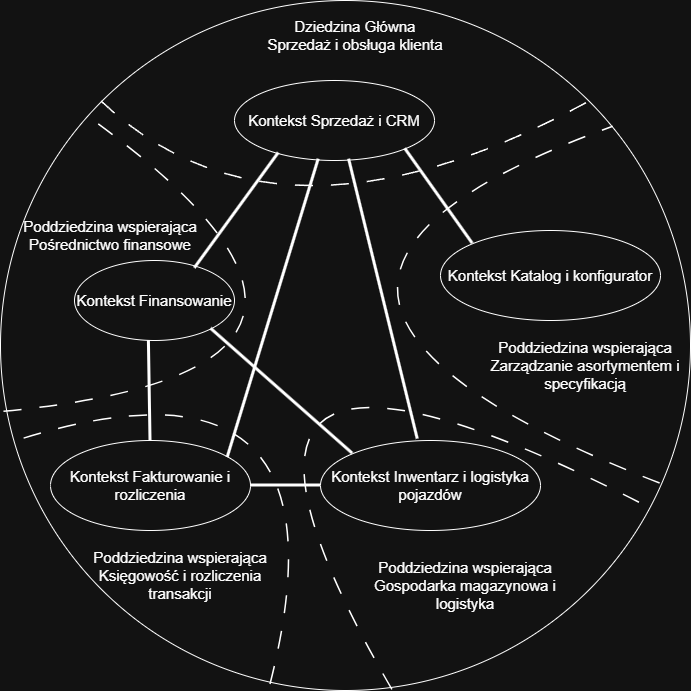
\includegraphics[width=\textwidth]{media/diagramy/mapa-kontekstow-final.png}
    \caption{Mapa kontekstów}
    \label{fig:hex_billing}
\end{figure}

\subsection{Konteksty ograniczone}

Aby zapobiec tworzeniu tzw. \textit{Big Ball of Mud} i umożliwić niezależny rozwój systemu, zdefiniowane wyżej poddziedziny biznesowe zostały odwzorowane w pięć kontekstów ograniczonych (obszarów rozwiązania IT). Granice każdego z nich wyznaczają zamknięty zakres obowiązywania języka wszechobecnego.

\begin{table}[H]
\centering
\small
\renewcommand{\arraystretch}{1.3}

\begin{tabular}{|p{3.2cm}|p{2cm}|p{3.5cm}|p{5.3cm}|}
\hline

\textbf{Poddziedzina} &
\textbf{Typ} &
\textbf{Kontekst Ograniczony} &
\textbf{Uzasadnienie}
\\
\hline

Sprzedaż i obsługa klienta &
Główna &
Sprzedaż i CRM &
Kontekst obejmuje relację z klientem, logikę ofertowania oraz cykl życia zamówienia.
\\
\hline

Zarządzanie asortymentem i specyfikacją &
Wspierająca &
Katalog i konfigurator &
Kontekst odpowiada za poprawność technologiczną specyfikacji, reguł wykluczeń oraz dystrybucję cenników.
\\
\hline

Gospodarka magazynowa i logistyka &
Wspierająca &
Inwentarz i logistyka pojazdów &
Kontekst odpowiada za fizyczne zarządzanie pojazdami na placu oraz śledzenie numerów VIN.
\\
\hline

Pośrednictwo finansowe &
Wspierająca &
Finansowanie &
Integracja z zewnętrznymi interfejsami (systemy bankowe oraz leasingodawców) realizowana przez bezpieczny wzorzec ACL.
\\
\hline

Księgowość i rozliczenia transakcji &
Wspierająca &
Fakturowanie i rozliczenia &
Obsługa dokumentów skarbowych (faktury VAT) oraz bezpieczna ewidencja wpłat i zadatków.
\\
\hline

\end{tabular}

\caption{Bezpośrednie mapowanie poddziedzin na konteksty ograniczone}
\label{tab:ddd_mapping}

\end{table}

\subsection{Context Mapping}
\begin{figure}[H]
    \centering
    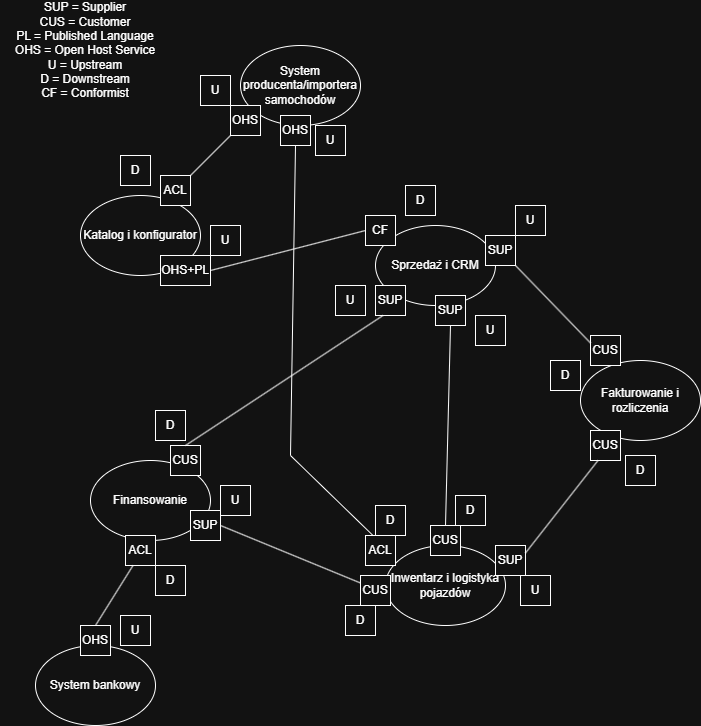
\includegraphics[width=\textwidth]{media/diagramy/contextmapfixed.png}
    \caption{Context Mapping}
    \label{fig:hex_billing}
\end{figure}

% --- Analiza domenowa | Język wszechobecny
\subsection{Język wszechobecny}
% =====================================================
% Język Wszechobecny - Sprzedaż i CRM
% =====================================================
\subsubsection{Kontekst: Sprzedaż i CRM}

\begin{longtable}{|p{4cm}|p{4cm}|p{8cm}|}
\hline
\textbf{Nazwa (PL)} & \textbf{Odpowiednik w kodzie (EN)} & \textbf{Opis} \\
\hline
\endfirsthead

\hline
\textbf{Nazwa (PL)} & \textbf{Odpowiednik w kodzie (EN)} & \textbf{Opis} \\
\hline
\endhead

Oferta & Offer & Sformalizowana, niewiążąca propozycja handlowa zawierająca specyfikację pojazdu oraz warunki finansowe. Służy do negocjacji i kalkulacji rabatów. \\
\hline

Zamówienie & Order & Formalne, twarde zobowiązanie zakupu pojazdu, powstające wyłącznie po akceptacji oferty przez klienta. Stanowi podstawę do uruchomienia procesów logistycznych i finansowych. \\
\hline

Sesja Konfiguratora & Configurator Session & Zewnętrzny proces technicznego doboru wyposażenia pojazdu, inicjowany przez CRM dla konkretnego klienta, kończący się zwróceniem gotowej specyfikacji. \\
\hline

Wydanie Pojazdu & Vehicle Handover & Finalna operacja w salonie (podpisanie protokołu i przekazanie kluczyków), zamykająca zamówienie i wymuszająca wyksięgowanie pojazdu z inwentarza. \\
\hline
\end{longtable}

% =====================================================
% Język Wszechobecny - Katalog i Konfigurator
% =====================================================
\subsubsection{Kontekst: Katalog i Konfigurator}

\begin{longtable}{|p{4cm}|p{4cm}|p{8cm}|}
\hline
\textbf{Nazwa (PL)} & \textbf{Odpowiednik w kodzie (EN)} & \textbf{Opis} \\
\hline
\endfirsthead

\hline
\textbf{Nazwa (PL)} & \textbf{Odpowiednik w kodzie (EN)} & \textbf{Opis} \\
\hline
\endhead

Katalog Produktów & Product Catalog & Kompletny zbiór opcji, pakietów i reguł zależności przypisany do danego rocznika modelowego. Pobierany zewnętrznie, obiekt ściśle niemutowalny w danej wersji. \\
\hline

Pakiet Wyposażenia & Equipment Package & Predefiniowany zbiór produktów (opcji) ułatwiający konfigurację, zapobiegający tzw. mikrozarządzaniu pojedynczymi elementami wyposażenia. \\
\hline

Układ Napędowy & Powertrain & Wymagana, podstawowa kombinacja wybranego silnika oraz kompatybilnej z nim skrzyni biegów. \\
\hline

Reguła Katalogowa & Catalog Rule & Zależność biznesowa blokująca tworzenie niedozwolonych przez fabrykę kombinacji sprzętowych lub wymuszająca dobranie brakujących opcji. \\
\hline

Specyfikacja & Vehicle Specification & Unikalna, budowana przez klienta konfiguracja pojazdu. Po osiągnięciu stanu kompletności staje się podstawą do wygenerowania oferty. \\
\hline
\end{longtable}

% =====================================================
% Język Wszechobecny - Inwentarz i Logistyka Pojazdów
% =====================================================
\subsubsection{Kontekst: Inwentarz i Logistyka Pojazdów}

\begin{longtable}{|p{4cm}|p{4cm}|p{8cm}|}
\hline
\textbf{Nazwa (PL)} & \textbf{Odpowiednik w kodzie (EN)} & \textbf{Opis} \\
\hline
\endfirsthead

\hline
\textbf{Nazwa (PL)} & \textbf{Odpowiednik w kodzie (EN)} & \textbf{Opis} \\
\hline
\endhead

Egzemplarz Pojazdu & Inventory Vehicle & Reprezentuje cykl życia pojazdu w ekosystemie dealera – łącząc fazę wirtualną (w produkcji) z fazą fizyczną (na placu). Identyfikowany przez numer VIN. \\
\hline

Plac & Stock & Lokalna baza pojazdów dostępnych fizycznie w salonie samochodowym. \\
\hline

Rezerwacja & Reservation & Przypisanie konkretnego numeru VIN do konkretnego zamówienia. Gwarantuje blokadę auta przed sprzedażą innemu klientowi. \\
\hline

Zlecenie Produkcji & Factory Order & Żądanie wysłane do zewnętrznego systemu fabryki w sytuacji, gdy samochodu o żądanej specyfikacji brakuje na lokalnym placu. \\
\hline

Timeout Rezerwacji & Reservation Timeout & Automatyczne zwolnienie rezerwacji pojazdu wywołane przekroczeniem terminu wpłaty zadatku lub zapłaty końcowej. \\
\hline

Wyksięgowanie & Inventory Release & Ostateczna zmiana statusu pojazdu zamykająca jego obecność na aktywnym stanie magazynowym dealera po wydaniu klientowi. \\
\hline
\end{longtable}

% =====================================================
% Język Wszechobecny - Finansowanie
% =====================================================
\subsubsection{Kontekst: Finansowanie}

\begin{longtable}{|p{4cm}|p{4cm}|p{8cm}|}
\hline
\textbf{Nazwa (PL)} & \textbf{Odpowiednik w kodzie (EN)} & \textbf{Opis} \\
\hline
\endfirsthead

\hline
\textbf{Nazwa (PL)} & \textbf{Odpowiednik w kodzie (EN)} & \textbf{Opis} \\
\hline
\endhead

Wniosek o Finansowanie & Financing Application & Zagregowany pakiet danych klienta i zamawianego pojazdu, wysyłany do zewnętrznej instytucji w celu weryfikacji zdolności kredytowej/leasingowej. \\
\hline

Decyzja Finansowa & Financing Decision & Ostateczny status (pozytywny lub negatywny) nadany przez bank, warunkujący możliwość kontynuowania procesu sprzedaży. \\
\hline

Warstwa Tłumacząca & Anti-Corruption Layer & Mechanizm izolujący rdzeń systemu, tłumaczący wewnętrzne zdarzenia domenowe na formaty zrozumiałe dla API konkretnego banku i odwrotnie. \\
\hline

System Bankowy & Bank System & Zewnętrzny decydent w kwestii przyznania środków; jedyne źródło prawdy o ostatecznym statusie wniosku kredytowego/leasingowego. \\
\hline
\end{longtable}

% =====================================================
% Język Wszechobecny - Fakturowanie i Rozliczenia
% =====================================================
\subsubsection{Kontekst: Fakturowanie i Rozliczenia}

\begin{longtable}{|p{4cm}|p{4cm}|p{8cm}|}
\hline
\textbf{Nazwa (PL)} & \textbf{Odpowiednik w kodzie (EN)} & \textbf{Opis} \\
\hline
\endfirsthead

\hline
\textbf{Nazwa (PL)} & \textbf{Odpowiednik w kodzie (EN)} & \textbf{Opis} \\
\hline
\endhead

Rozliczenie & Settlement & Agregat będący centralnym mechanizmem kontroli finansowej kontraktu. Śledzi wpłaty i pilnuje, czy zamówienie zostało w pełni opłacone. \\
\hline

Proforma & Proforma & Dokument skarbowy, pełniący rolę wezwania do zapłaty (wygenerowany na potrzeby wpłaty zadatku). \\
\hline

Faktura & Invoice & Prawnie wiążący dokument sprzedaży wystawiany po potwierdzeniu rezerwacji pojazdu. \\
\hline

Zadatek & Advance Payment & Bezzwrotna wpłata początkowa, wymagana do potwierdzenia zamówienia produkcyjnego lub rezerwacji auta z placu. \\
\hline

Należność & Receivable & Całkowita kwota pieniędzy z tytułu kontraktu, której dealer oczekuje od klienta. \\
\hline

Saldo & Balance & Obliczana na bieżąco różnica pomiędzy całkowitą należnością a sumą dotychczas zaksięgowanych wpłat. \\
\hline

Płatność Częściowa & Partial Payment & Status rozliczenia oznaczający, że zarejestrowana wpłata (lub wpłaty) jest niższa od całkowitej oczekiwanej kwoty salda. \\
\hline

Rozliczone & Settled & Docelowy stan rozliczenia, w którym saldo zamówienia wynosi równe 0 PLN, co stanowi zielone światło do fizycznego wydania pojazdu. \\
\hline
\end{longtable}

% --- Analiza domenowa | Wizja wymagań :?

\subsection{Wymagania funkcjonalne}

\subsubsection{Kontekst: Sprzedaż i CRM}
\begin{itemize}
    \item \textbf{WF-SPR-01} --- System musi umożliwiać prowadzenie procesu sprzedaży pojazdu od ofertowania do wydania.
    \item \textbf{WF-SPR-02} --- System musi zarządzać cyklem życia zamówienia klienta.
    \item \textbf{WF-SPR-03} --- System musi obsługiwać różne formy płatności za pojazd.
\end{itemize}

\subsubsection{Kontekst: Katalog i konfigurator}
\begin{itemize}
    \item \textbf{WF-KAT-01} --- System musi umożliwiać konfigurację pojazdu zgodnie z regułami producenta.
    \item \textbf{WF-KAT-02} --- System musi zapewniać aktualność katalogu modeli i cenników.
\end{itemize}

\subsubsection{Kontekst: Inwentarz i logistyka pojazdów}
\begin{itemize}
    \item \textbf{WF-INW-01} --- System musi zarządzać stanem magazynowym pojazdów na placu salonu samochodowego.
    \item \textbf{WF-INW-02} --- System musi obsługiwać proces zamawiania i przyjęcia pojazdu z fabryki.
    \item \textbf{WF-INW-03} --- System musi kontrolować rezerwacje pojazdów i zapobiegać ich podwójnej sprzedaży.
\end{itemize}

\subsubsection{Kontekst: Finansowanie}
\begin{itemize}
    \item \textbf{WF-FIN-01} --- System musi umożliwiać składanie i obsługę wniosków o finansowanie pojazdu.
    \item \textbf{WF-FIN-02} --- System musi integrować się z zewnętrznymi instytucjami finansowymi.
\end{itemize}

\subsubsection{Kontekst: Fakturowanie i rozliczenia}
\begin{itemize}
    \item \textbf{WF-FIR-01} --- System musi generować dokumenty księgowe dla transakcji sprzedaży.
    \item \textbf{WF-FIR-02} --- System musi ewidencjonować wpłaty klientów i rozliczać salda zamówień.
    \item \textbf{WF-FIR-03} --- System musi monitorować i egzekwować terminy płatności.
\end{itemize}

% --- Analiza domenowa | DDD Storytelling

\input{sections/analiza-domenowa/ddd-storytelling}

\subsection{Bounded context canvas}
\begin{figure}[H]
    \centering
    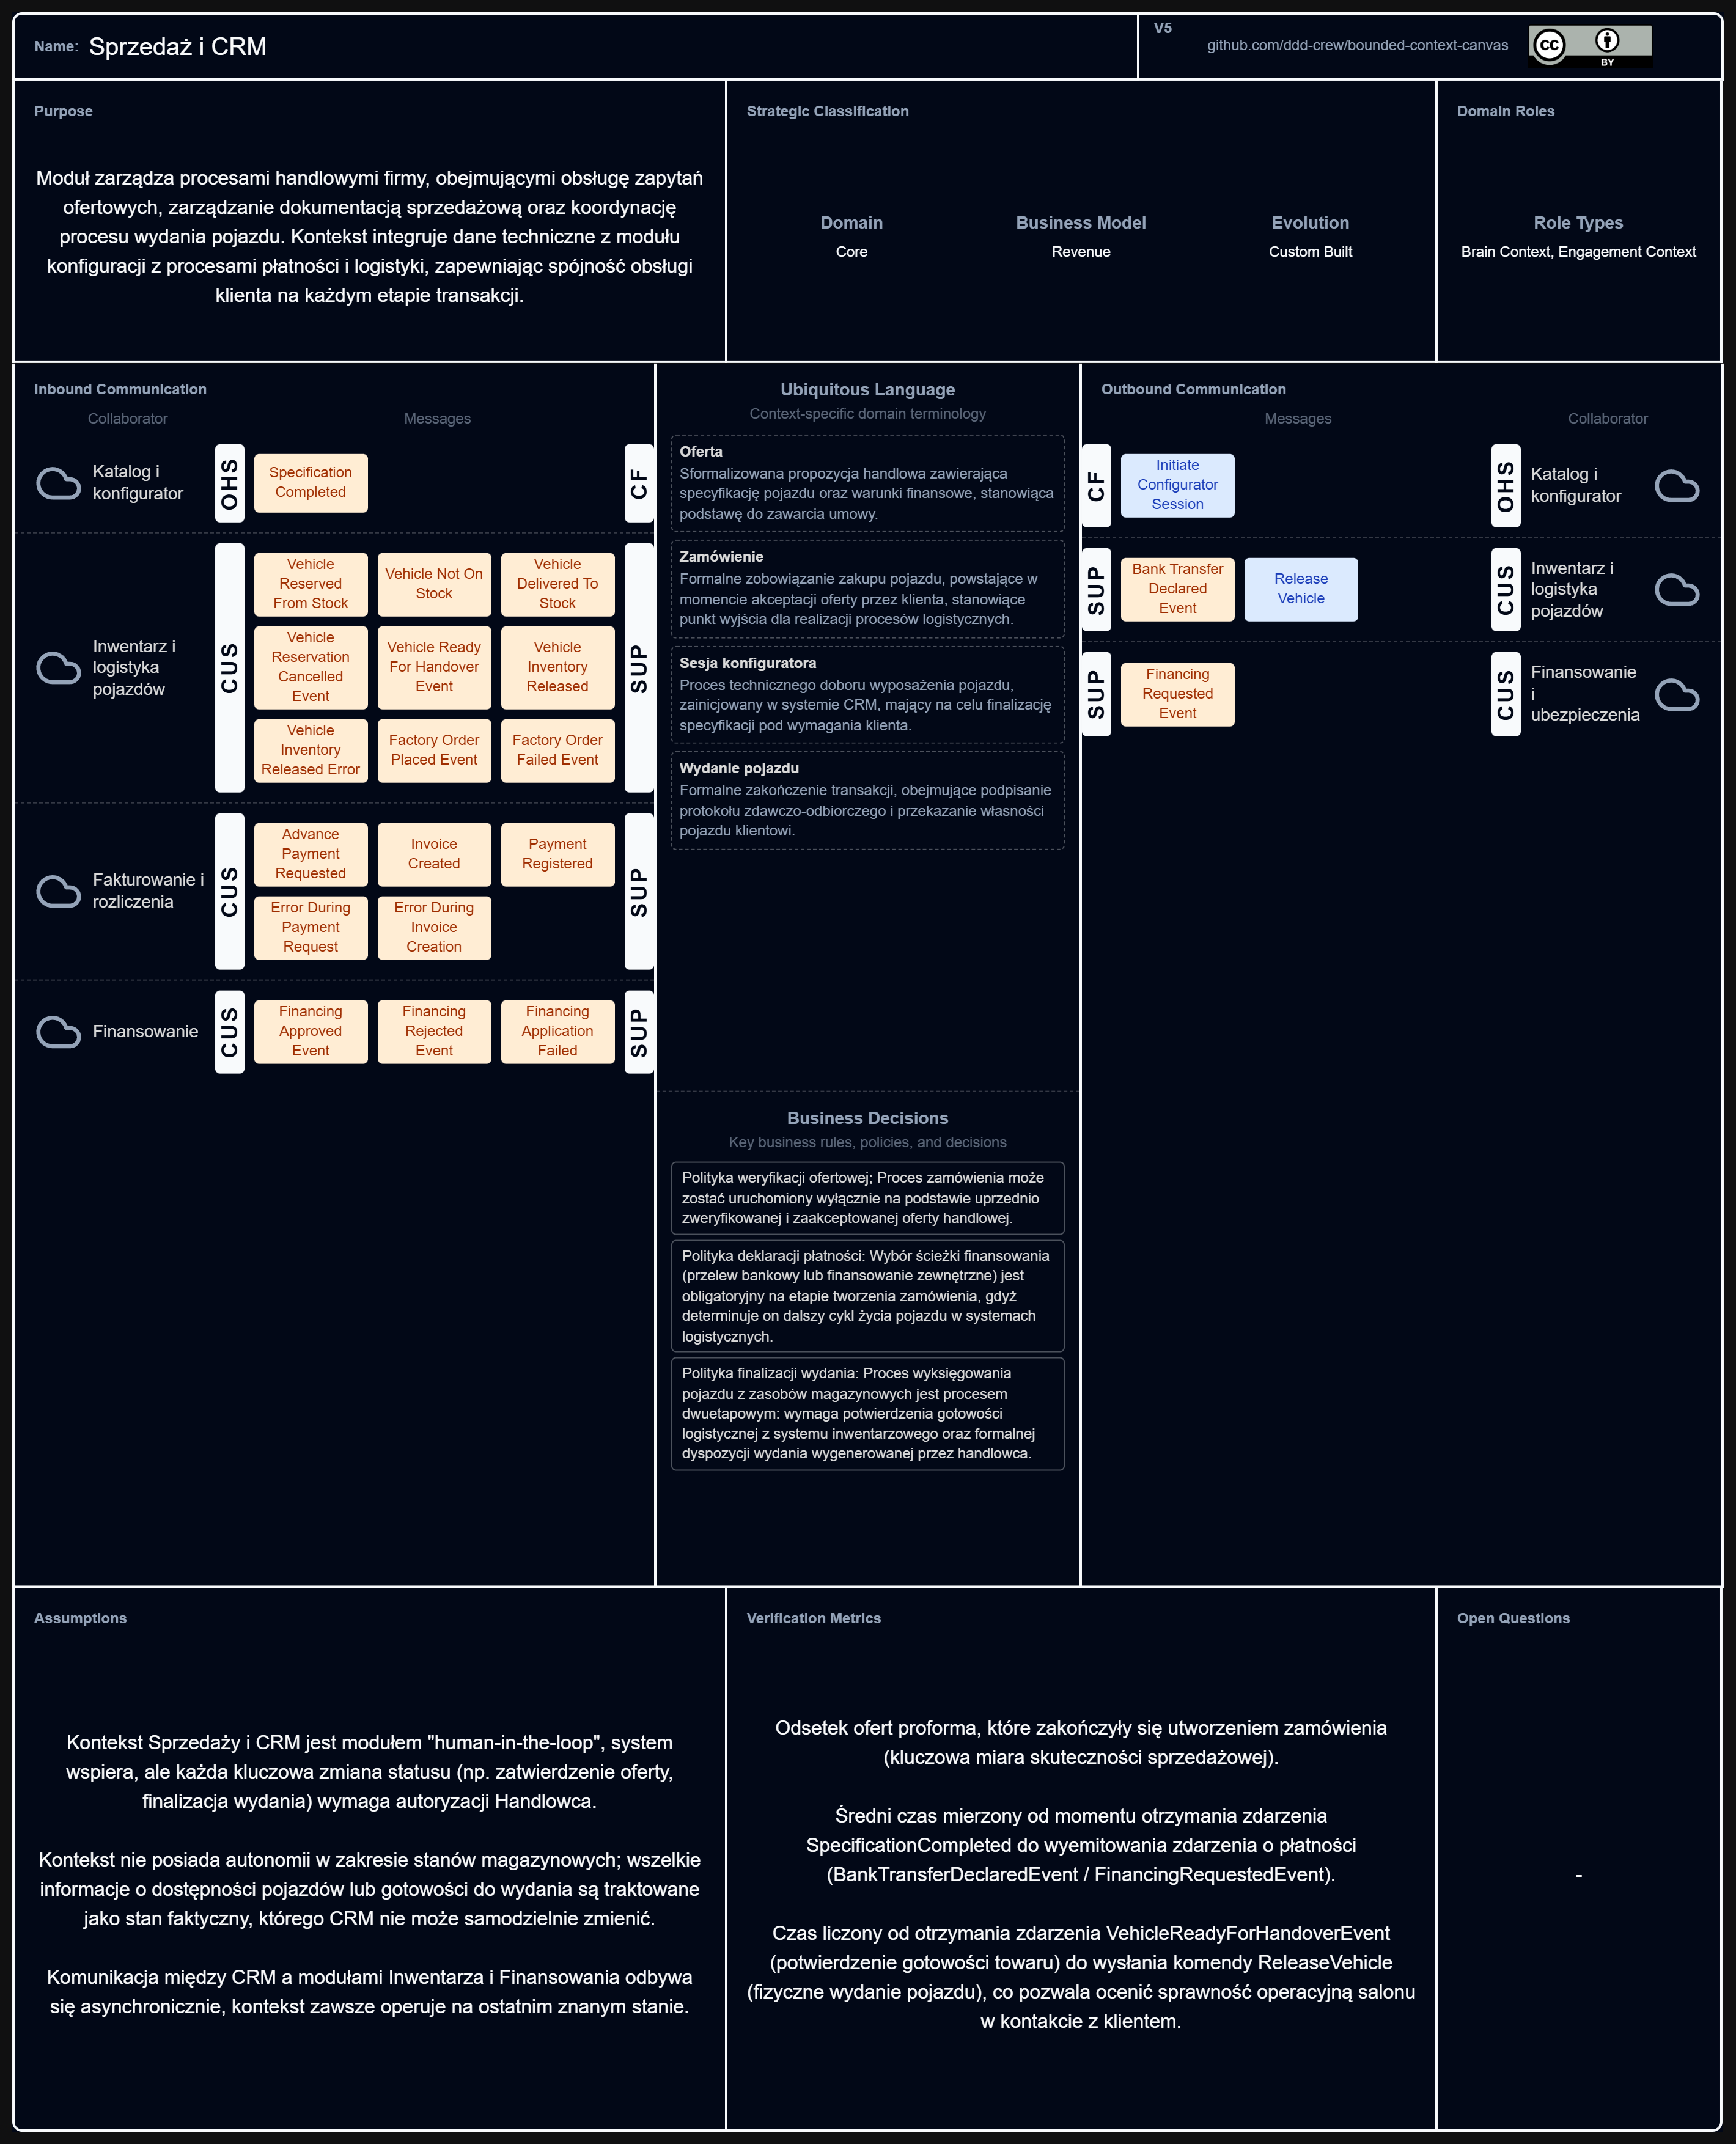
\includegraphics[width=\textwidth]{media/bounded-context-canvas/final/SIC_K1_TOTAL_FINAL.png}
    \caption{Kanwa Kontekstu Sprzedaży i CRM}
    \label{fig:hex_billing}
\end{figure}

\begin{figure}[H]
    \centering
    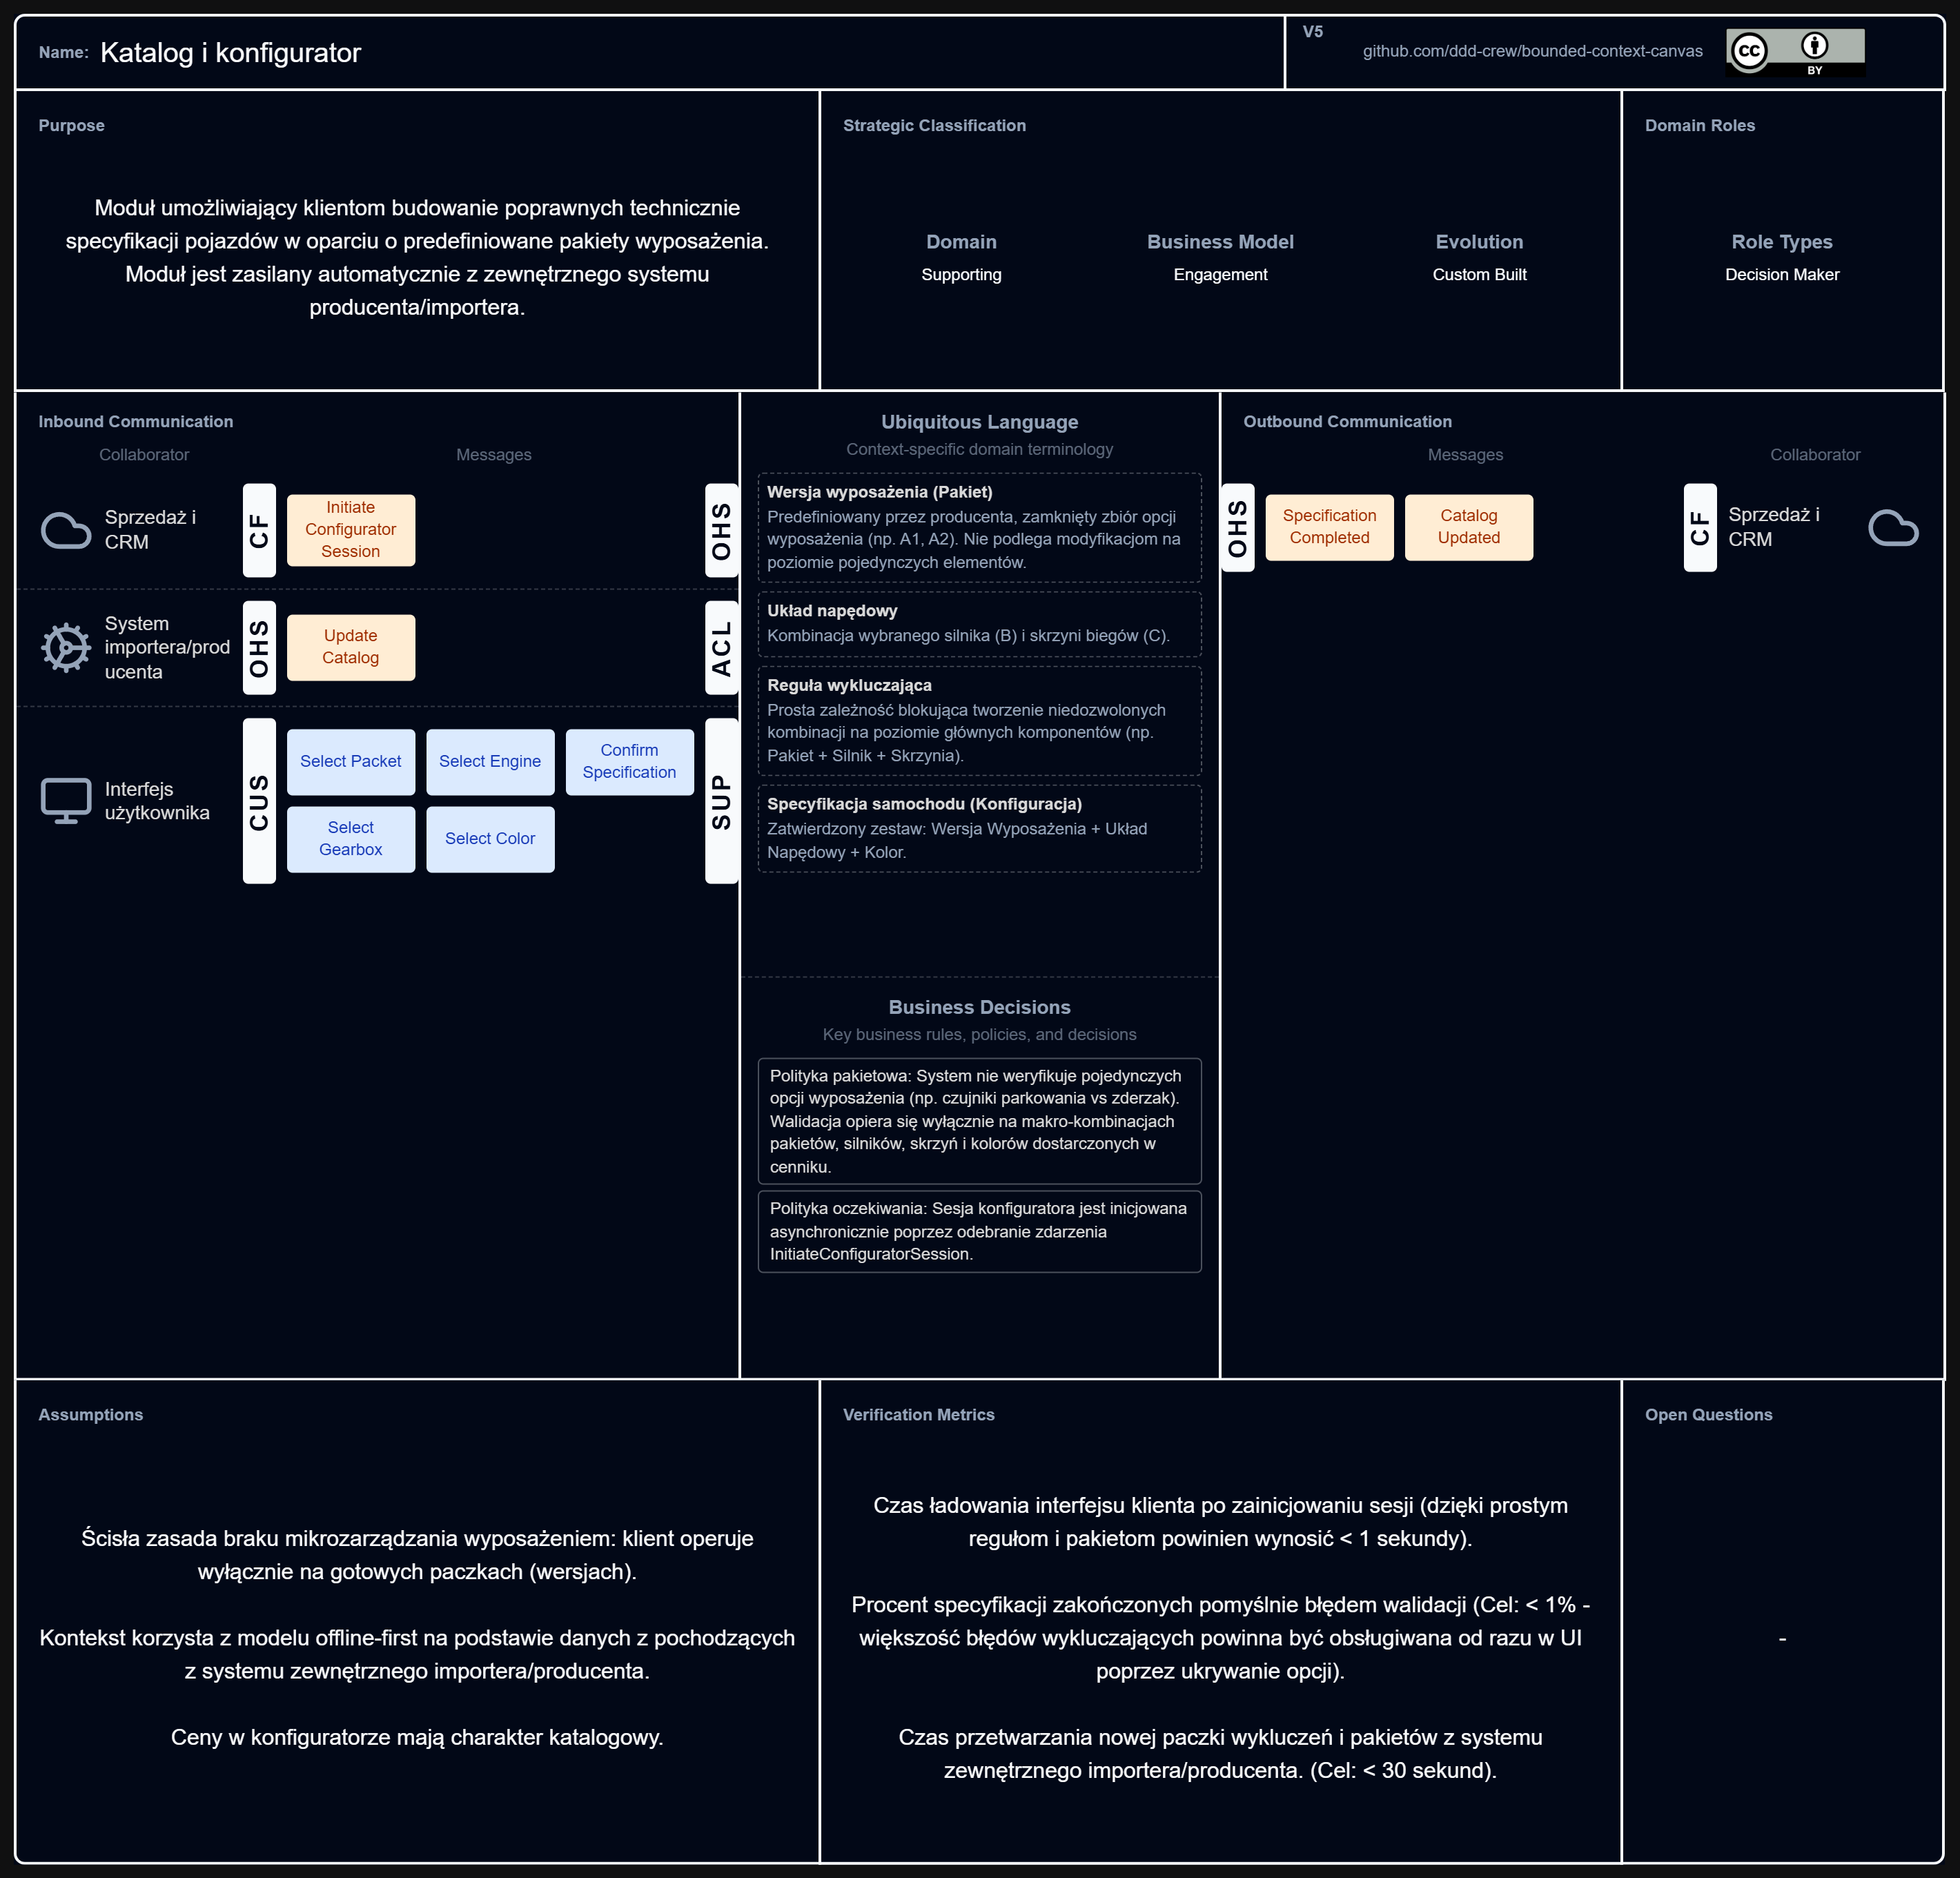
\includegraphics[width=\textwidth]{media/bounded-context-canvas/final/KIK_K2_TOTAL_FINAL.png}
    \caption{Kanwa Kontekstu Katalogu i konfiguratora}
    \label{fig:hex_billing}
\end{figure}

\begin{figure}[H]
    \centering
    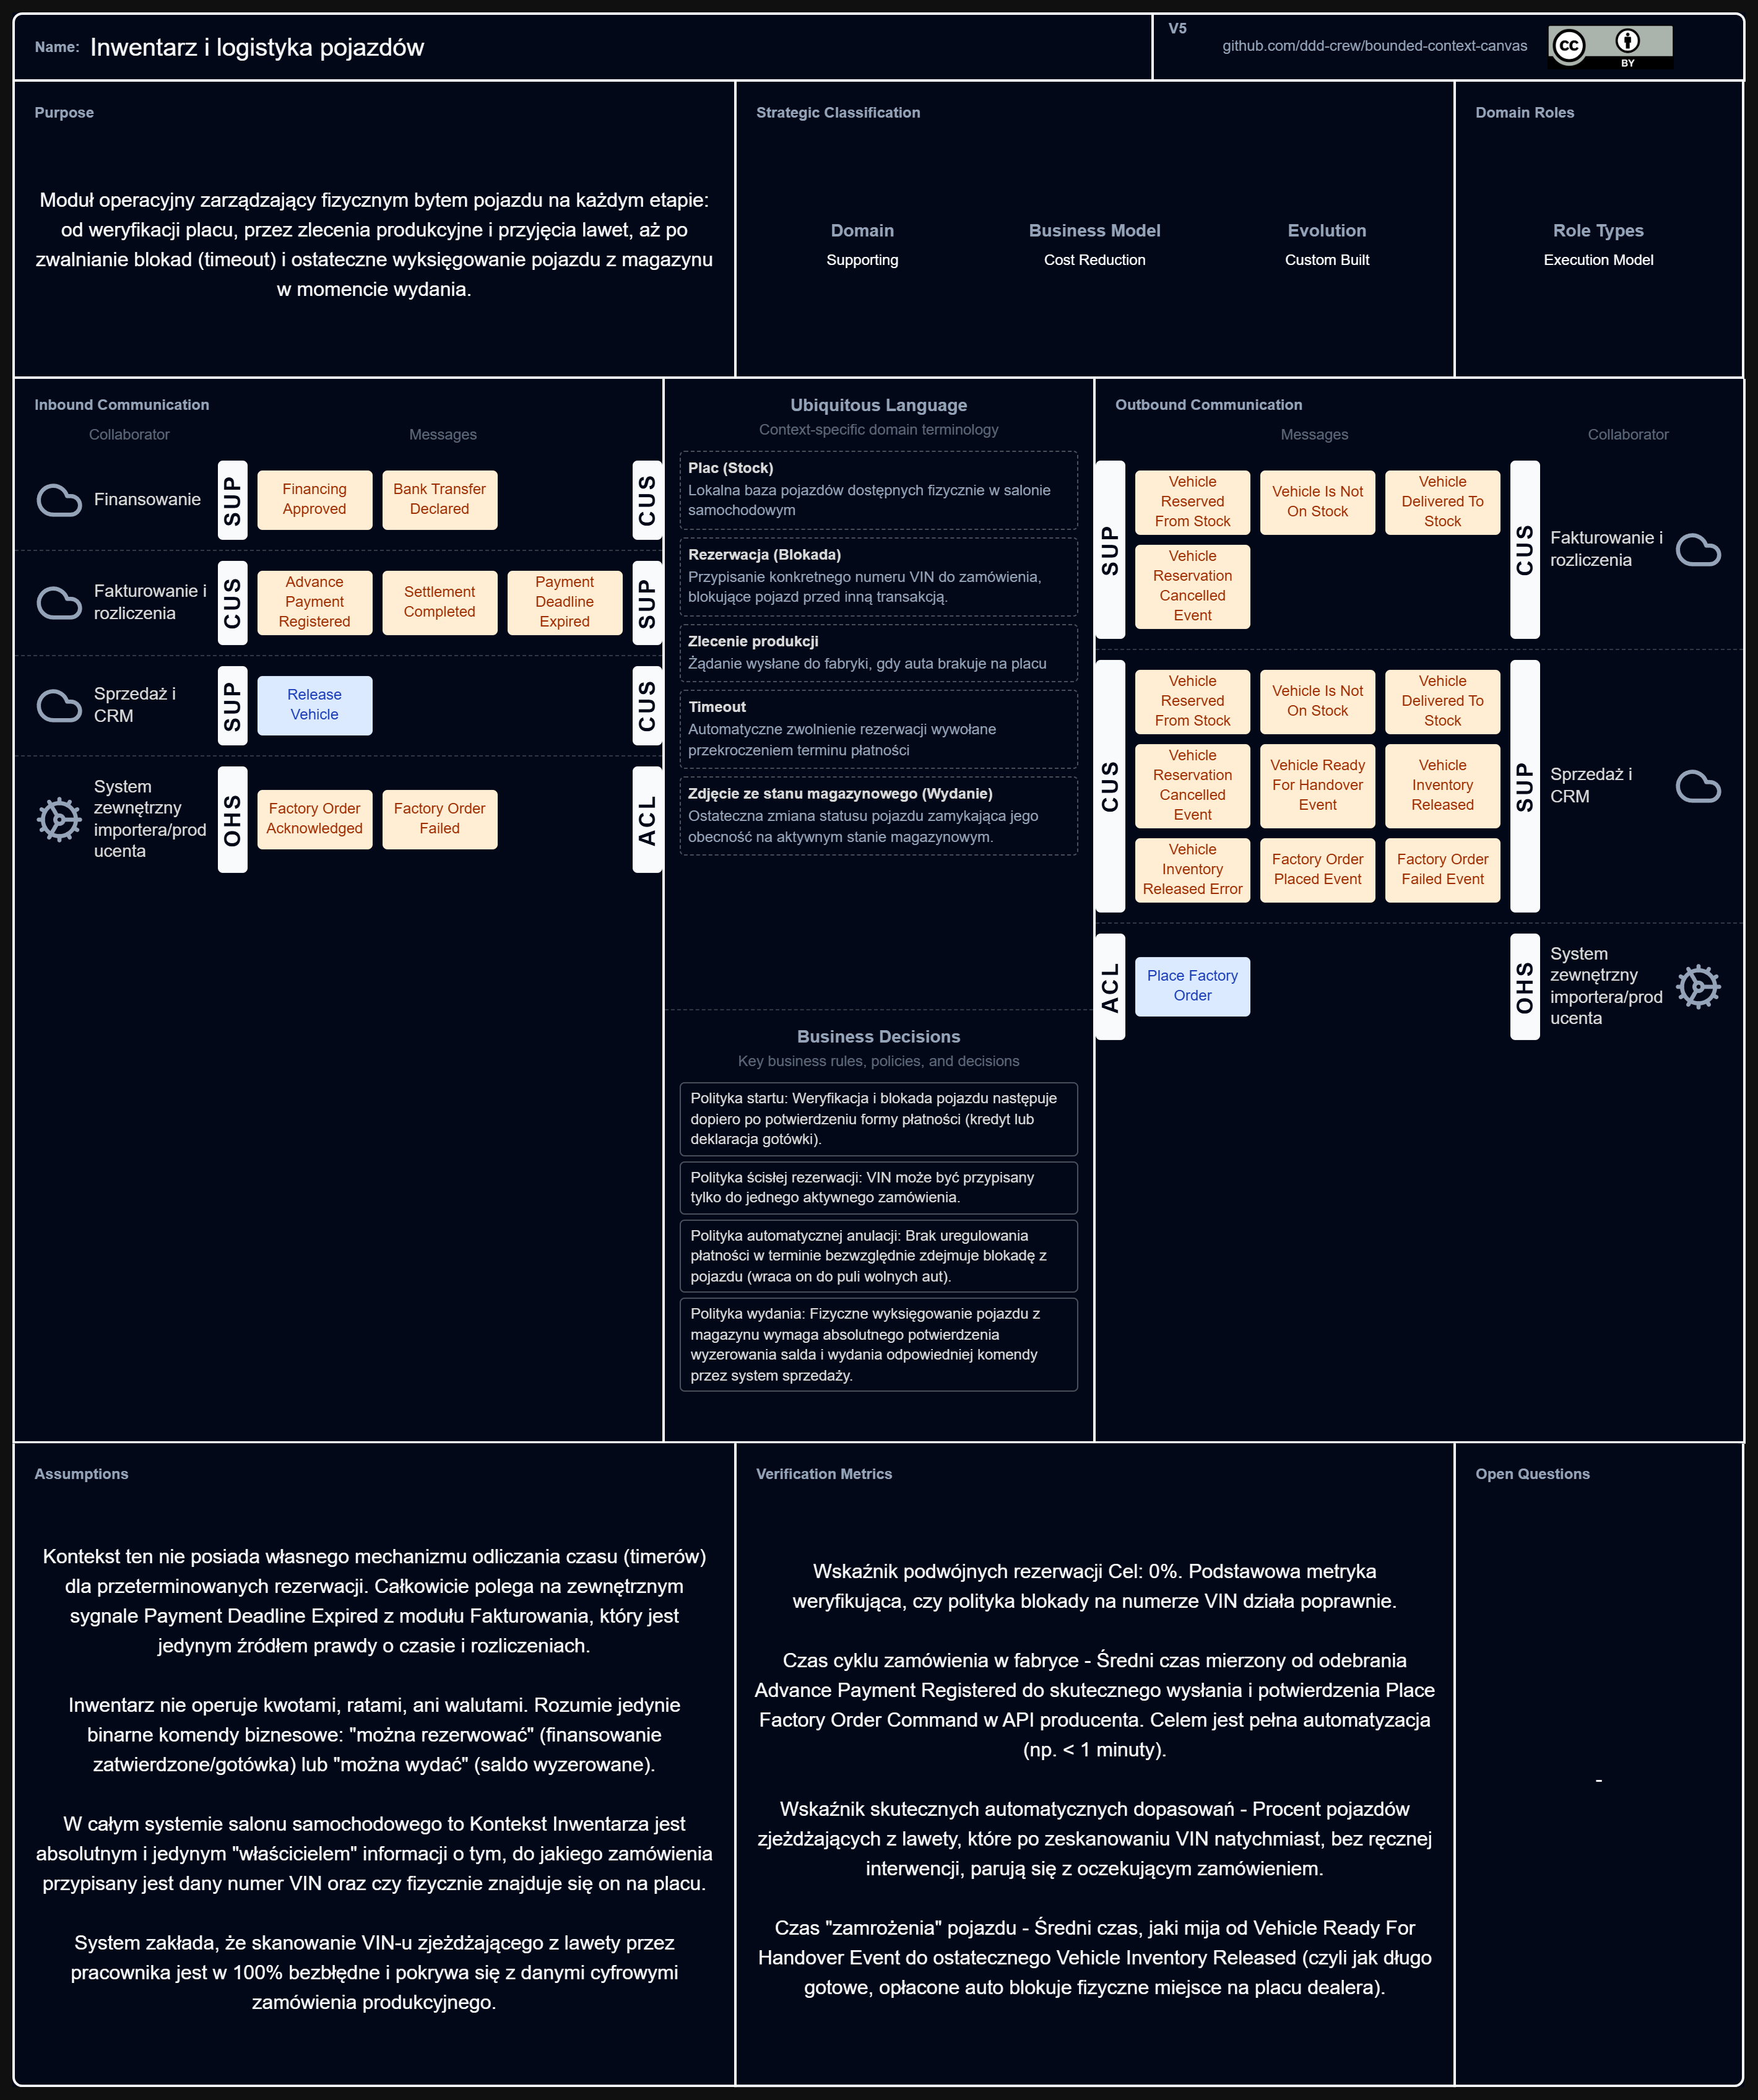
\includegraphics[width=\textwidth]{media/bounded-context-canvas/final/IiLP_K3_TOTAL_FINAL.png}
    \caption{Kanwa Kontekstu Inwentarza i Logistyki pojazdów}
    \label{fig:hex_billing}
\end{figure}

\begin{figure}[H]
    \centering
    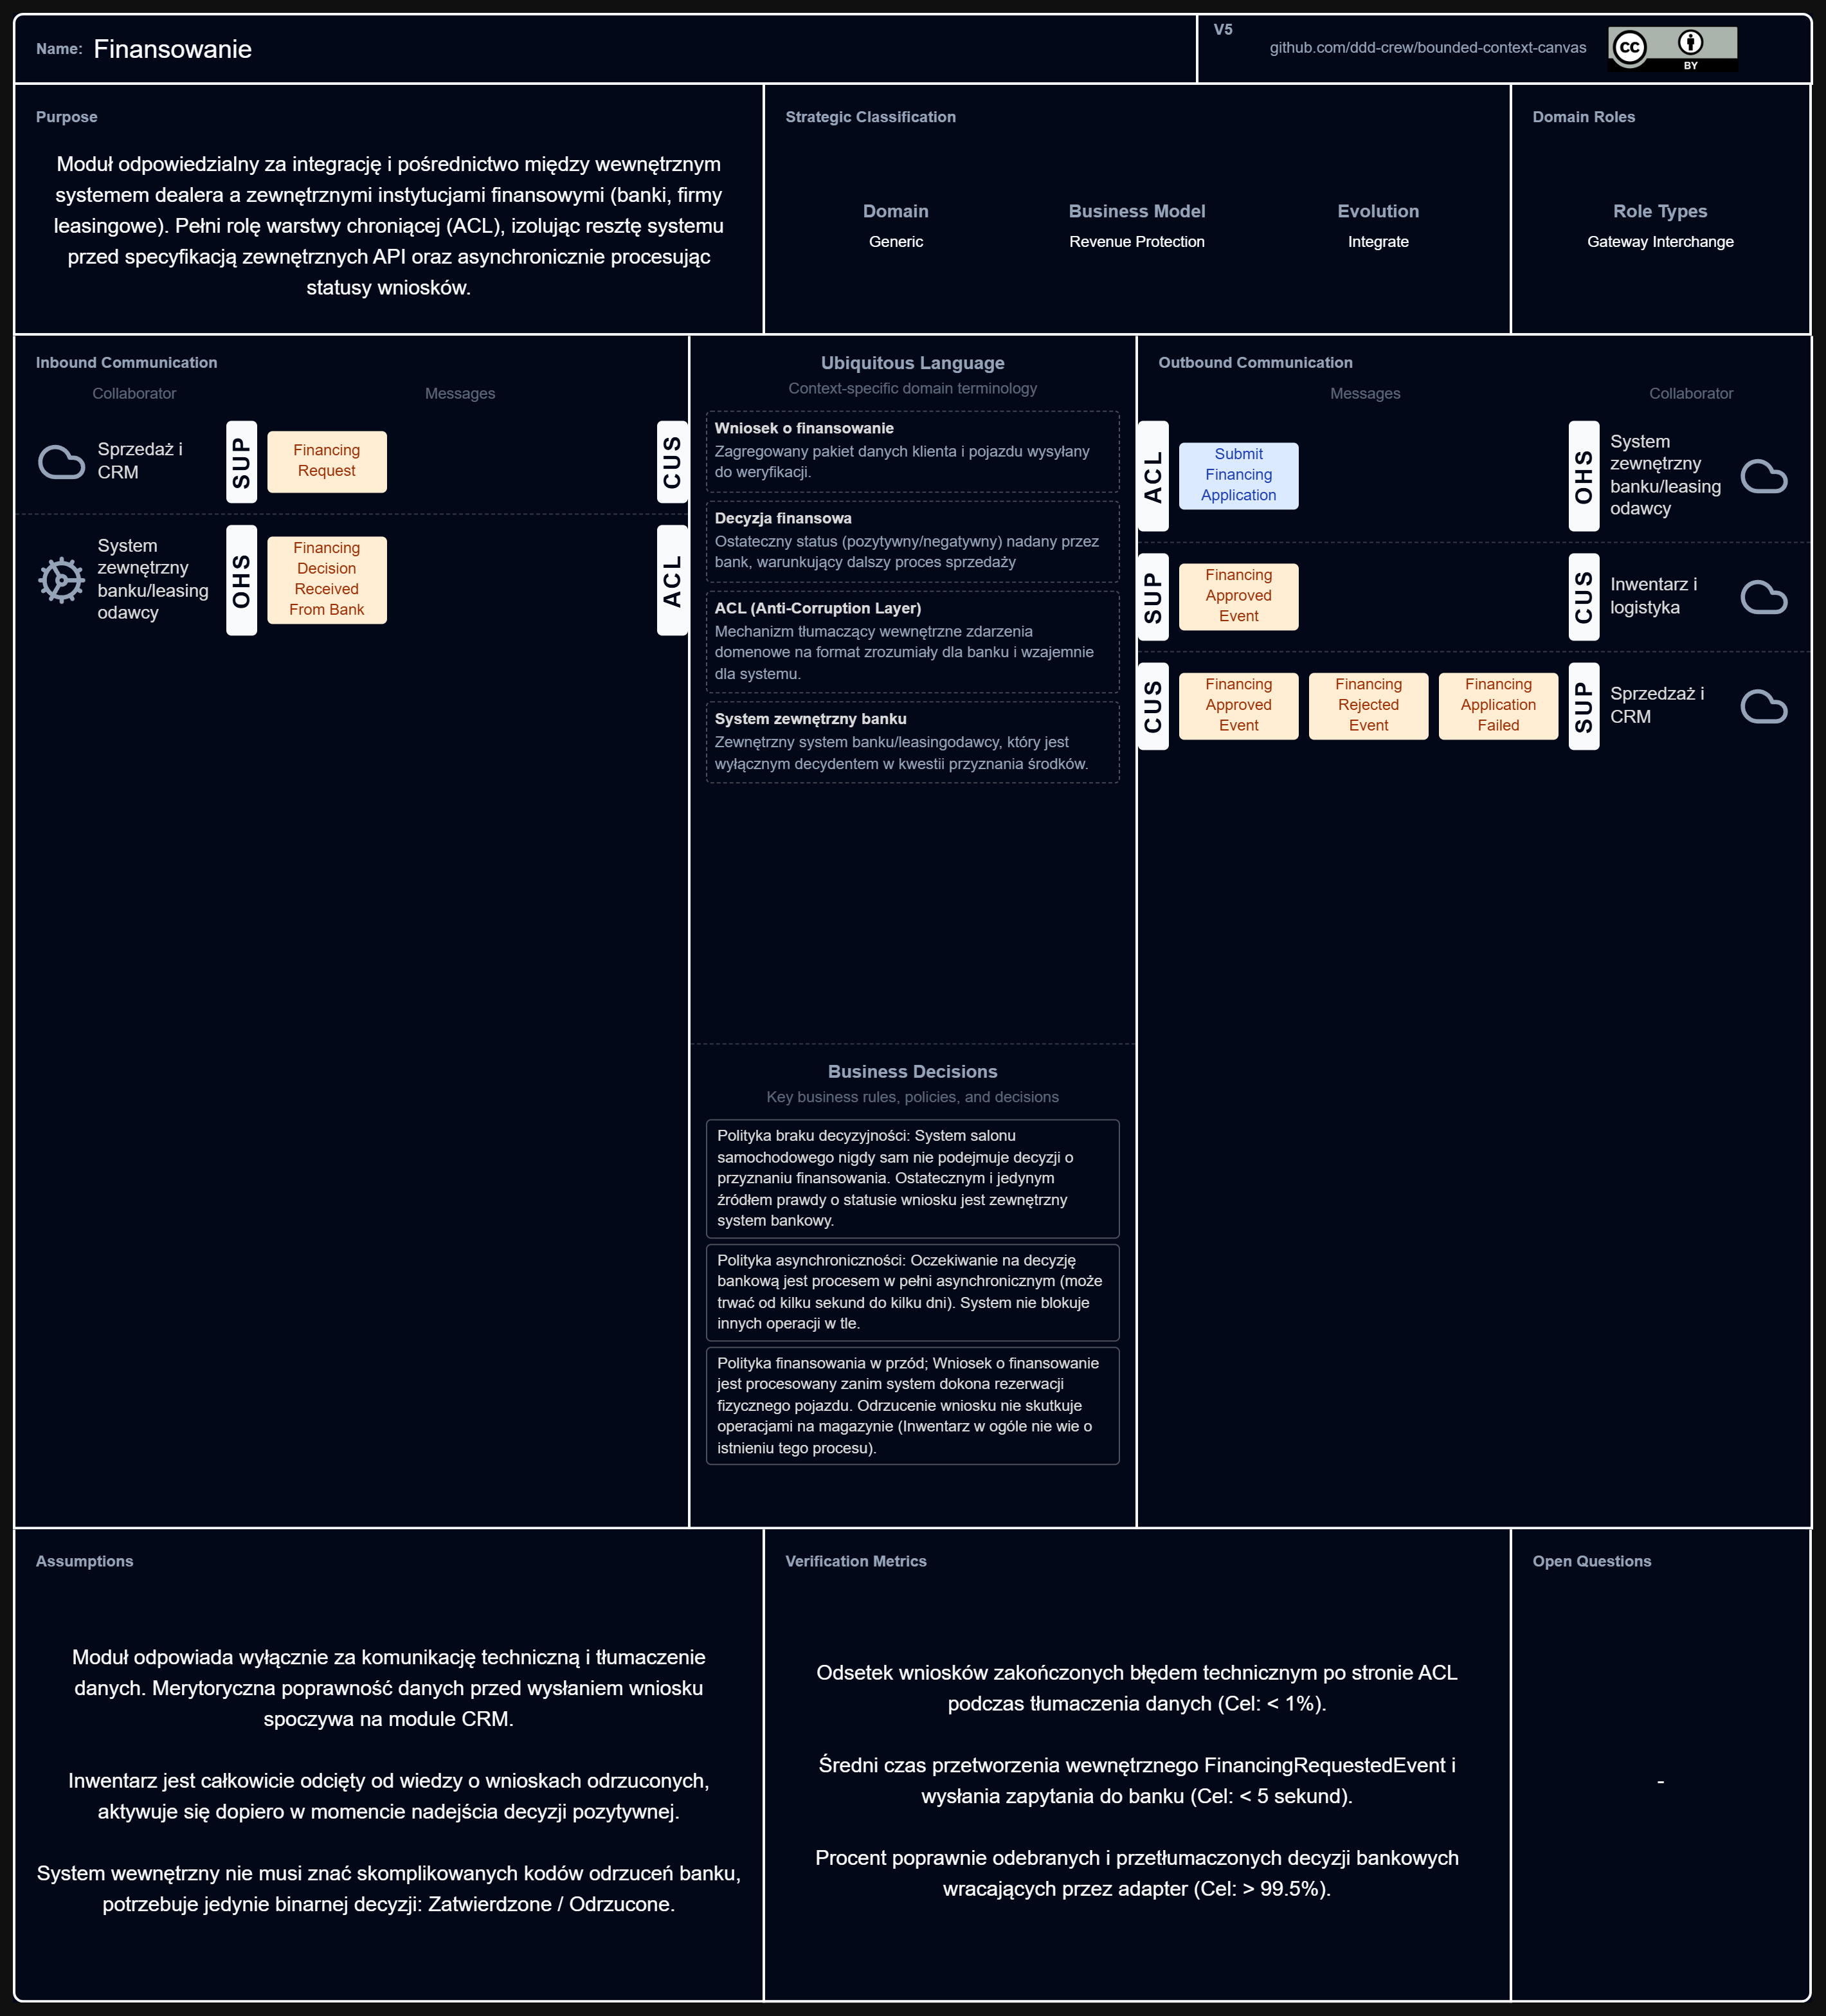
\includegraphics[width=\textwidth]{media/bounded-context-canvas/after_review/finansowanie_v5.png}
    \caption{Kanwa Kontekstu Finansowania}
    \label{fig:hex_billing}
\end{figure}

\begin{figure}[H]
    \centering
    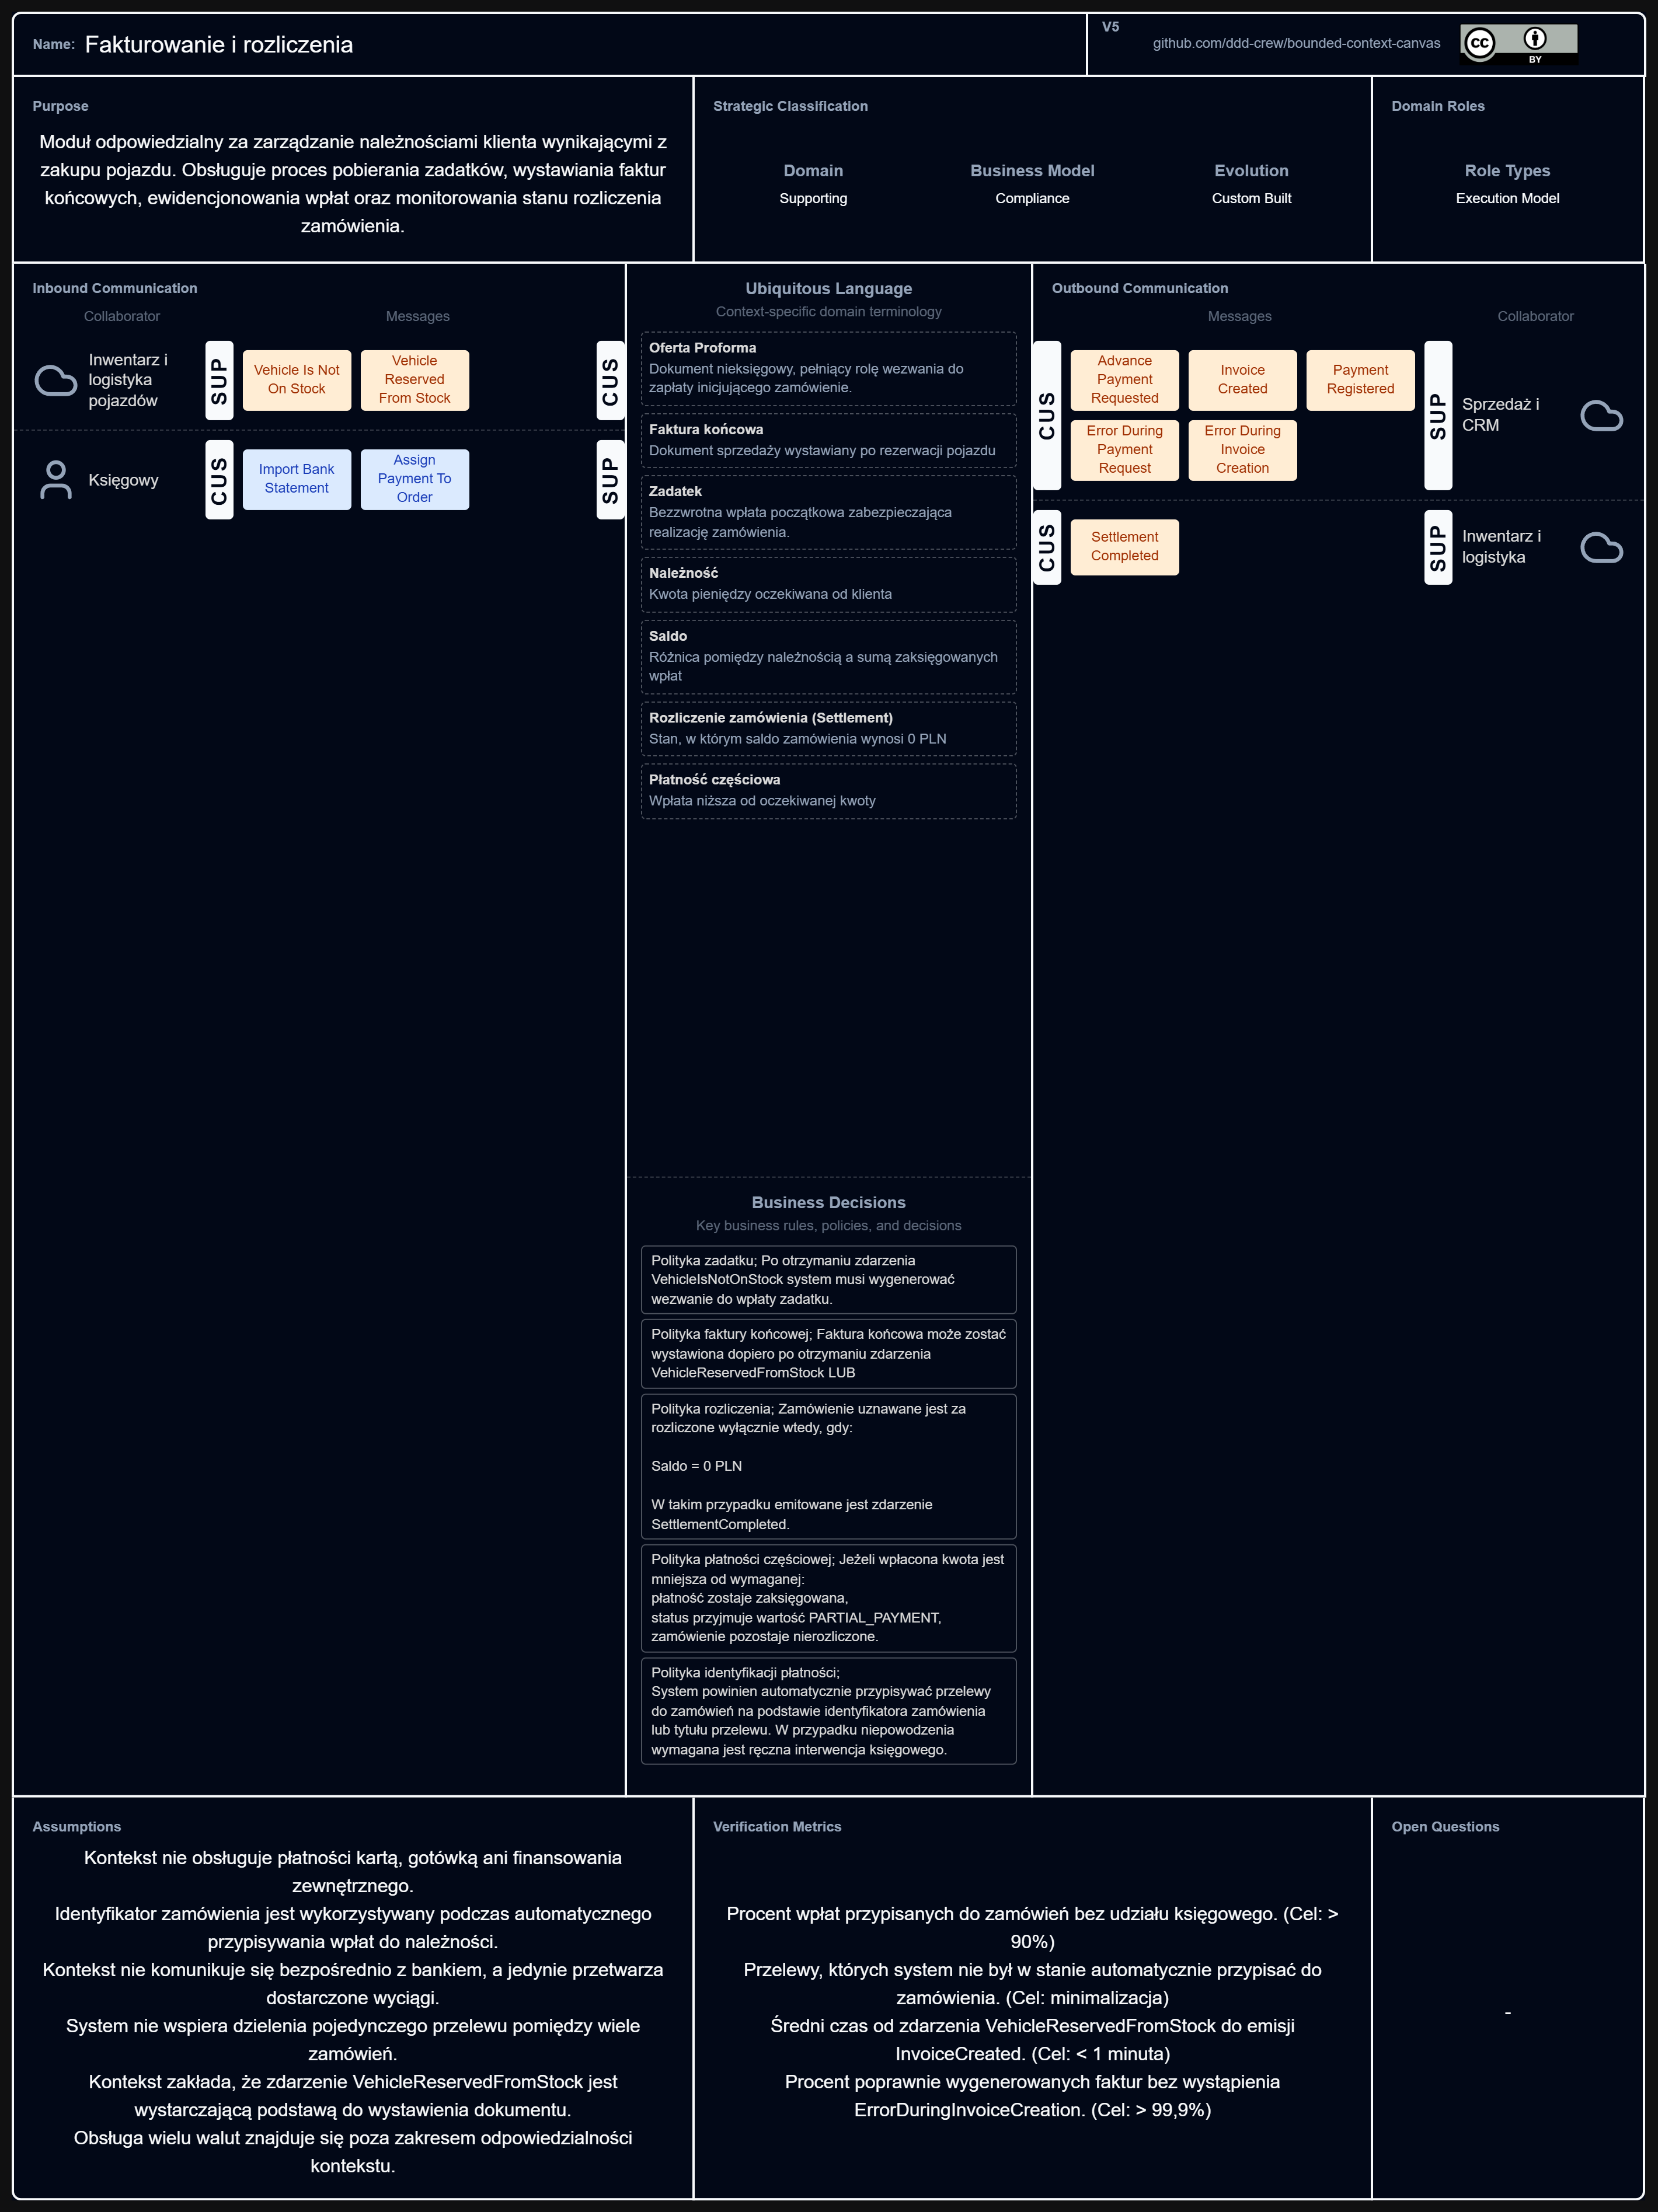
\includegraphics[width=\textwidth]{media/bounded-context-canvas/final/FIR_K7_TOTAL_FINAL.png}
    \caption{Kanwa Kontekstu Fakturowania i Rozliczeń}
    \label{fig:hex_billing}
\end{figure}


\subsection{Event storming}
W celu zapewnienia optymalnej czytelności oraz precyzyjnego odwzorowania cyklu życia domeny biznesowej, ostateczny model wypracowany podczas sesji Event Stormingowej został zaprezentowany w formie podziału na sekwencyjne etapy. Należy jednak stanowczo podkreślić, że \textbf{przedstawione na kolejnych schematach fazy nie są odizolowanymi procesami, lecz stanowią jeden, spójny i chronologiczny ciąg zdarzeń biznesowych} modelowanego systemu DMS.

Podział na odrębne grafiki (Etapy 1-5 oraz gałąź asynchroniczną) podyktowany jest wysoką złożonością domeny i naturalnym przechodzeniem odpowiedzialności pomiędzy poszczególnymi Kontekstami Ograniczonymi (Sprzedaż, Katalog, Finansowanie, Fakturowanie oraz Inwentarz).

Całościowy przepływ (\textit{Domain Flow}) realizowany jest w sposób ciągły:
\begin{itemize}
    \item \textbf{Etap 1 i 2} obrazują początek osi czasu: od pierwszej interakcji klienta w konfiguratorze, aż po wygenerowanie wiążącego zamówienia i kluczowe rozwidlenie ścieżki płatności (gotówka lub finansowanie zewnętrzne).
    
    \item \textbf{Etap 3 i 4} to płynna kontynuacja procesu, w której na podstawie gwarancji finansowej z poprzednich kroków, system uruchamia operacje magazynowo-logistyczne (rezerwacja na placu lub zlecenie do fabryki po opłaceniu zadatku), kończąc się wystawieniem faktury i pełnym rozliczeniem.
    
    \item \textbf{Etap 5} stanowi zwieńczenie głównego strumienia transakcji, w którym w pełni opłacony i gotowy logistycznie pojazd jest fizycznie wydawany klientowi, zamykając cykl życia zamówienia.
    
    \item Dopełnieniem całości jest wyodrębniona \textbf{Gałąź asynchroniczna}, która działa w tle jako mechanizm zabezpieczający (wyzwalany upływem czasu), mogący w dowolnym momencie przerwać główny ciąg w przypadku braku uregulowania należności przez klienta.
\end{itemize}

Takie sekwencyjne podejście pozwala śledzić stan nadrzędnych agregatów (takich jak \textit{Zamówienie} czy \textit{Egzemplarz Pojazdu}) przechodzących przez kolejne maszyny stanów w ramach całego zintegrowanego procesu salonu samochodowego.

\begin{figure}[H]
    \centering
    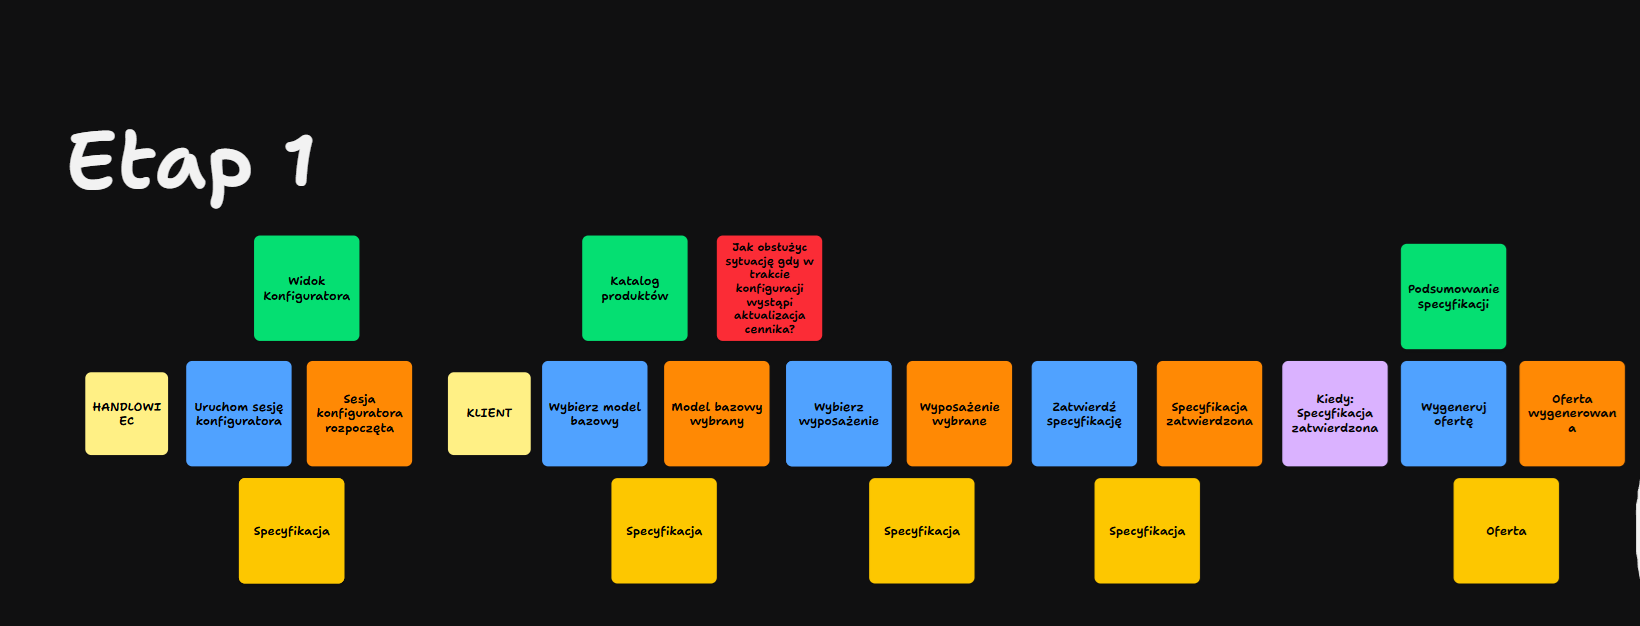
\includegraphics[width=\textwidth]{media/event-storming-poprawiony/Event_stormingE1.png}
    \caption{Etap 1: Konfiguracja pojazdu oraz wygenerowanie oferty}
    \label{fig:es_etap1}
\end{figure}

\begin{figure}[H]
    \centering
    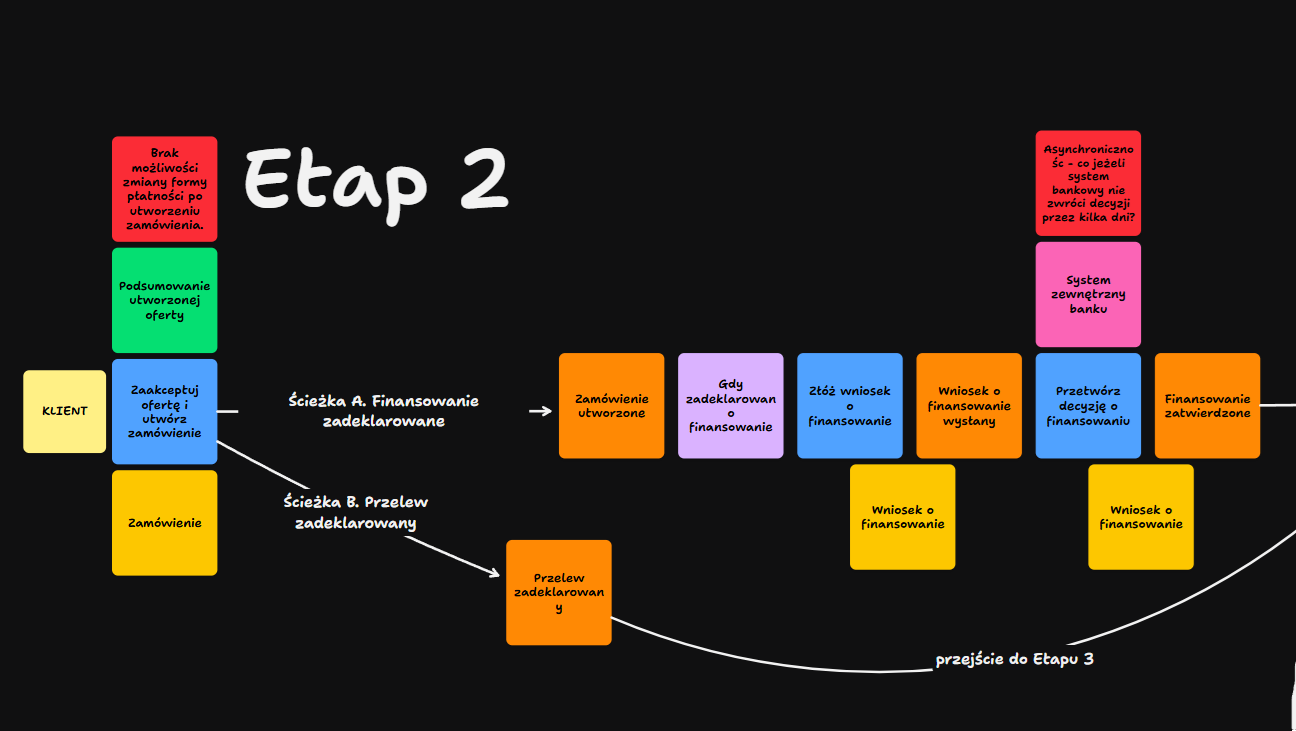
\includegraphics[width=\textwidth]{media/event-storming-poprawiony/Event_stormingE2.png}
    \caption{Etap 2: Utworzenie zamówienia i wybór ścieżki płatności}
    \label{fig:es_etap2}
\end{figure}

\begin{figure}[H]
    \centering
    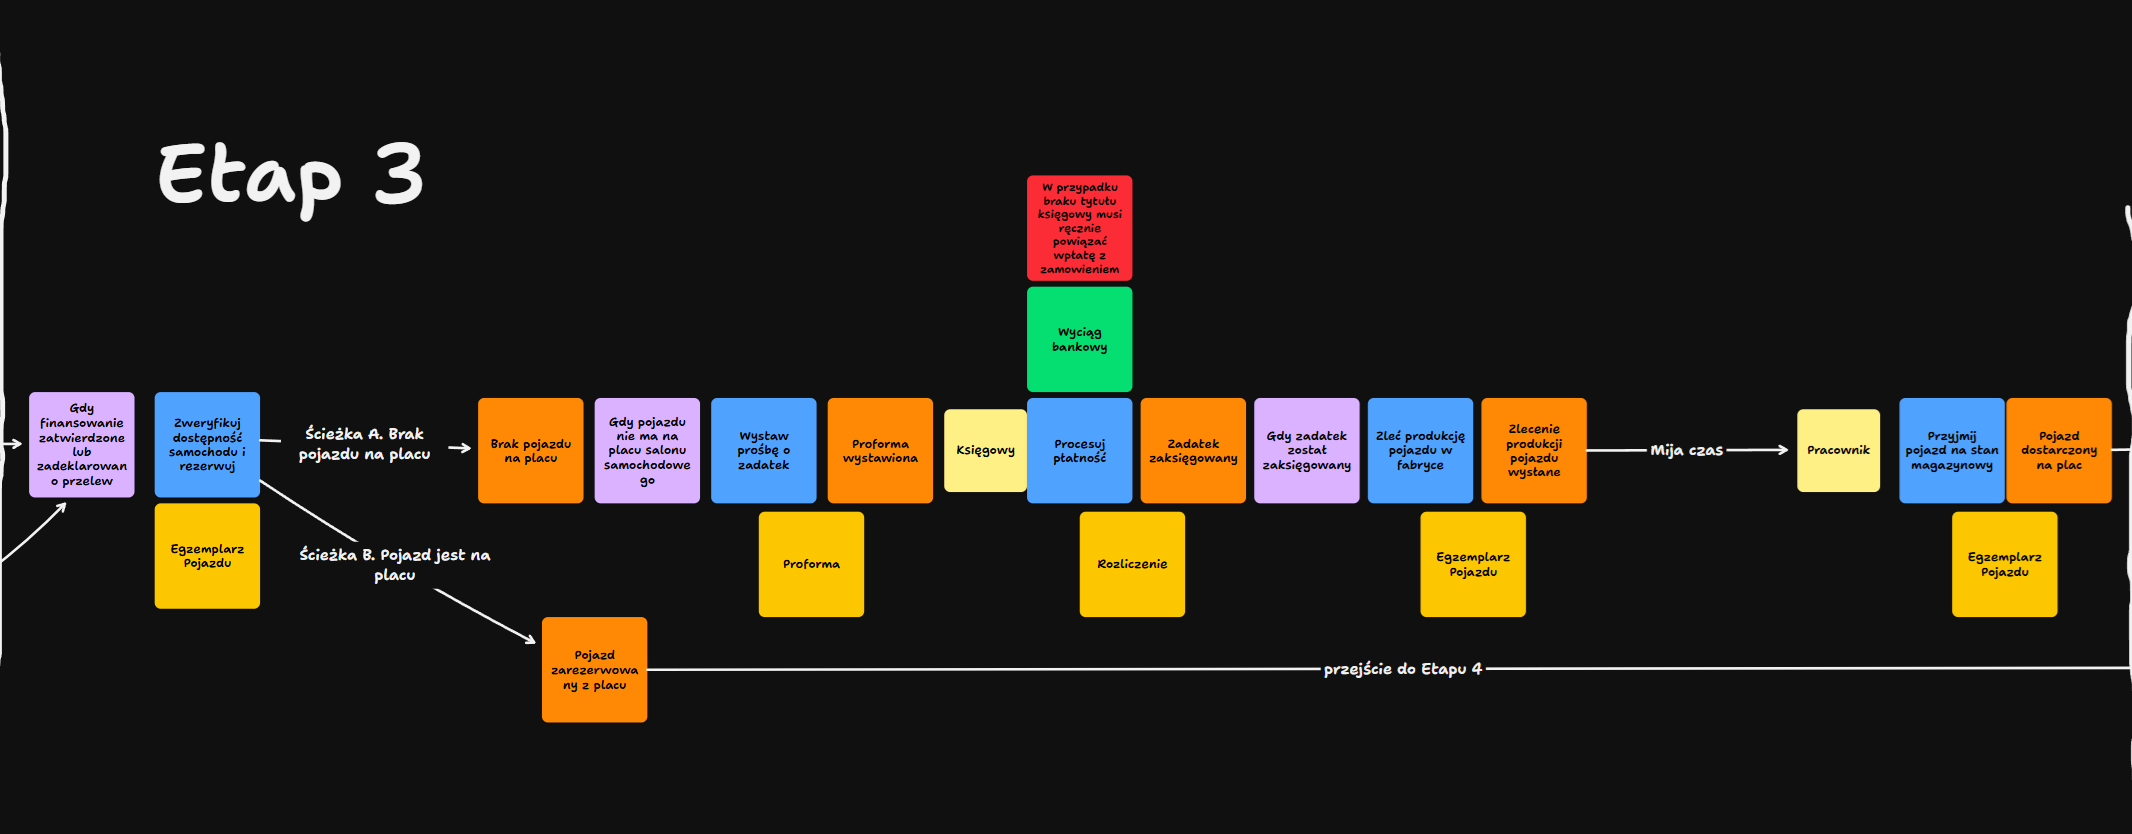
\includegraphics[width=\textwidth]{media/event-storming-poprawiony/Event_stormingE3.png}
    \caption{Etap 3: Weryfikacja placu, proces bankowy oraz zlecenia fabryczne}
    \label{fig:es_etap3}
\end{figure}

\begin{figure}[H]
    \centering
    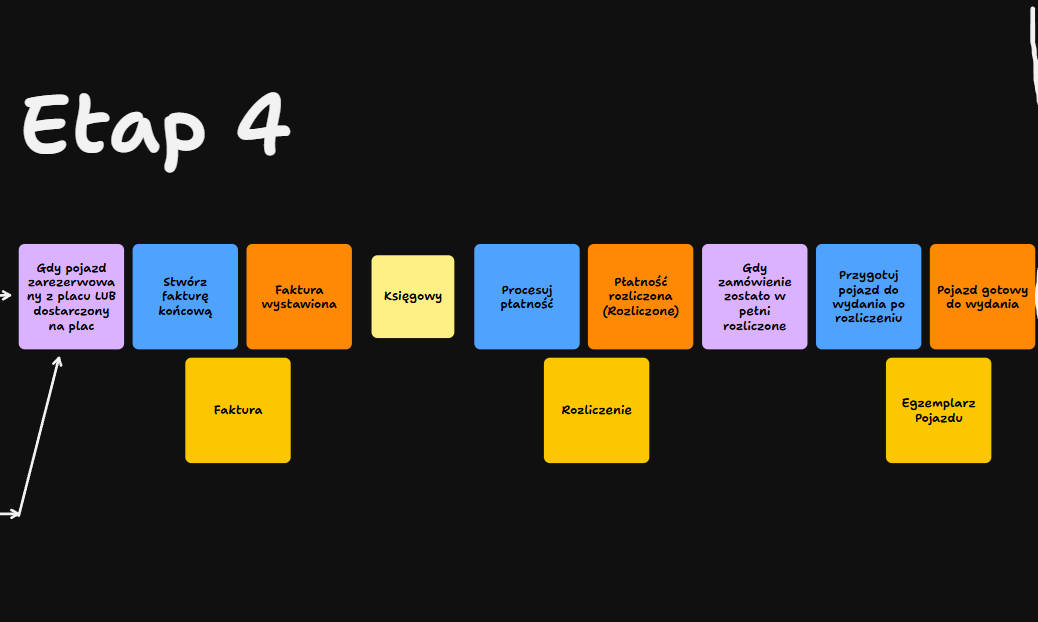
\includegraphics[width=\textwidth]{media/event-storming-poprawiony/Event_stormingE4.png}
    \caption{Etap 4: Fakturowanie końcowe i pełne rozliczenie zamówienia}
    \label{fig:es_etap4}
\end{figure}

\begin{figure}[H]
    \centering
    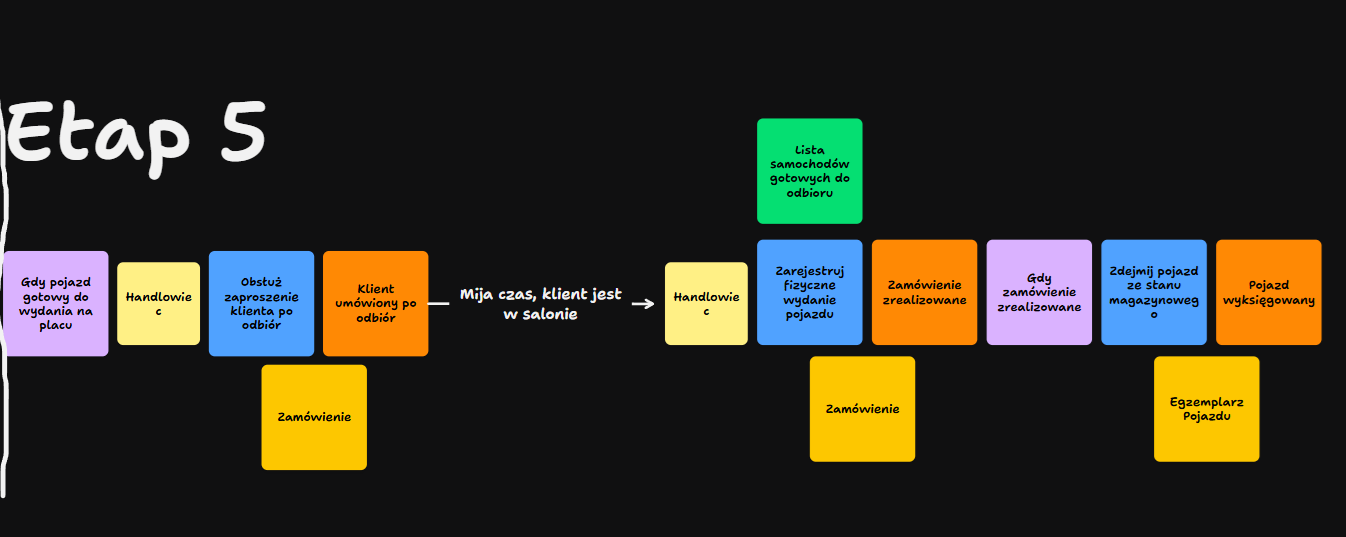
\includegraphics[width=\textwidth]{media/event-storming-poprawiony/Event_stormingE5.png}
    \caption{Etap 5: Fizyczne wydanie pojazdu i wyksięgowanie ze stanu magazynowego}
    \label{fig:es_etap5}
\end{figure}

\begin{figure}[H]
    \centering
    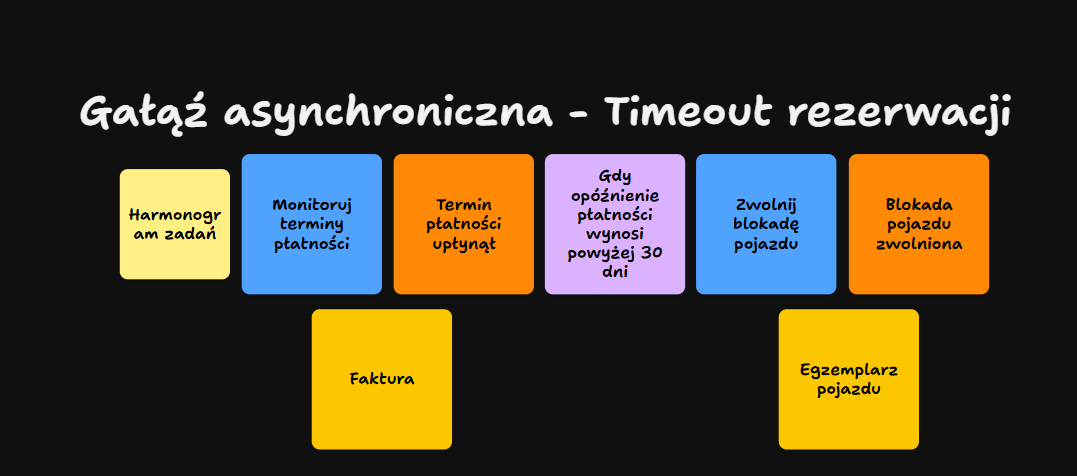
\includegraphics[width=\textwidth]{media/event-storming-poprawiony/Event_stormingE6.png}
    \caption{Gałąź asynchroniczna: Monitorowanie terminów płatności i zwolnienie blokady (Timeout)}
    \label{fig:es_etap6}
\end{figure}

% --- Analiza domenowa | Przypadki uzycia

% \subsection{Przypadki użycia}
% \newpage
% \subsubsection{Kontekst; Sprzedaż i CRM}
% % =====================================================
\textbf{UC-CRM-01: Uruchomienie sesji konfiguratora dla klienta}

\begin{longtable}{|p{4cm}|p{11cm}|}
\hline
\textbf{Element} & \textbf{Opis} \\
\hline

Identyfikator & UC-CRM-01 \\
\hline

Nazwa & Uruchomienie sesji konfiguratora dla klienta \\
\hline

Opis & 
Zainicjowanie nowej szansy sprzedaży poprzez wygenerowanie i otwarcie dedykowanej sesji w konfiguratorze pojazdów, przypisanej do konkretnego klienta i handlowca. \\
\hline

Aktor główny & Handlowiec \\
\hline

Aktorzy pomocniczy & - \\
\hline

Warunki wstępne & 
Klient wykazuje zainteresowanie zakupem nowego pojazdu. \\
\hline

Warunki końcowe & 
Wygenerowana zostaje nowa sesja, a kontekst emituje zdarzenie \textit{InitiateConfiguratorSession}. \\
\hline

Scenariusz główny & 
\begin{enumerate}
    \item Handlowiec wybiera opcję konfiguracji nowego pojazdu dla tego klienta.
    \item Kontekst emituje zdarzenie inicjujące \textit{InitiateConfiguratorSession}.
    \item System otwiera w nowym widoku interfejs konfiguratora (z modułu Katalogu).
\end{enumerate} \\
\hline

Scenariusze alternatywne & 
\begin{itemize}
    \item [] Brak.
\end{itemize} \\
\hline
\end{longtable}

% =====================================================
\textbf{UC-CRM-02: Wygenerowanie oferty proforma}

\begin{longtable}{|p{4cm}|p{11cm}|}
\hline
\textbf{Element} & \textbf{Opis} \\
\hline

Identyfikator & UC-CRM-02 \\
\hline

Nazwa & Wygenerowanie oferty proforma \\
\hline

Opis & 
Proces utworzenia wstępnej oferty handlowej w systemie na podstawie danych (specyfikacji, ceny oraz danych kontaktowych klienta) otrzymanych w payloadzie zdarzenia z konfiguratora. \\
\hline

Aktor główny & Handlowiec \\
\hline

Aktorzy pomocniczy & - \\
\hline

Warunki wstępne & 
Kontekst otrzymał zdarzenie \textit{SpecificationCompleted} zawierające pełną konfigurację, wyliczoną cenę oraz dane identyfikacyjne klienta. \\
\hline

Warunki końcowe & 
Nowa Oferta zostaje utworzona i zapisana w systemie ze statusem "W przygotowaniu". \\
\hline

Scenariusz główny & 
\begin{enumerate}
    \item System powiadamia handlowca o nowej specyfikacji oczekującej na ofertowanie.
    \item Handlowiec otwiera formularz nowej oferty.
    \item Handlowiec uzupełnia ofertę o dane klienta. Informacje o specyfikacji i cenie katalogowej uzupełniane są bezpośrednio z otrzymanego zdarzenia.
    \item Handlowiec generuje dokument oferty proforma zmieniając status na 'Utworzona' i prezentuje go klientowi.
\end{enumerate} \\
\hline

Scenariusze alternatywne & 
\begin{itemize}
    \item [] Brak.
\end{itemize} \\
\hline
\end{longtable}

% =====================================================
\textbf{UC-CRM-03: Zatwierdzenie oferty i utworzenie zamówienia}

\begin{longtable}{|p{4cm}|p{11cm}|}
\hline
\textbf{Element} & \textbf{Opis} \\
\hline

Identyfikator & UC-CRM-03 \\
\hline

Nazwa & Zatwierdzenie oferty, utworzenie zamówienia i wybór formy płatności \\
\hline

Opis & 
Proces akceptacji wygenerowanej oferty przez klienta oraz utworzenia na jej podstawie nowego zamówienia (osobnego agregatu), co uruchamia właściwe procesy logistyczne i sprzedażowe. \\
\hline

Aktor główny & Handlowiec \\
\hline

Aktorzy pomocniczy & Klient \\
\hline

Warunki wstępne & 
Wygenerowana i ważna oferta proforma (agregat Oferta) istnieje w systemie CRM. \\
\hline

Warunki końcowe & 
Oferta otrzymuje status "Zaakceptowana". W systemie powstaje nowe Zamówienie ze statusem "W realizacji", a system emituje odpowiednie zdarzenie inicjujące weryfikację stanu magazynowego placu lub proces bankowy. \\
\hline

Scenariusz główny & 
\begin{enumerate}
    \item Klient akceptuje warunki przedstawione na ofercie proforma.
    \item Handlowiec zmienia status oferty na "Zaakceptowana" w systemie CRM.
    \item Handlowiec tworzy nowe zamówienie na podstawie zaakceptowanej oferty.
    \item Handlowiec wprowadza na zamówieniu zadeklarowaną przez klienta formę płatności (Przelew lub Finansowanie).
    \item System CRM emituje zdarzenie \textit{BankTransferDeclaredEvent} (dla przelewu) LUB \textit{FinancingRequestedEvent} (dla finansowania).
\end{enumerate} \\
\hline

Scenariusze alternatywne & 
\begin{itemize}
    \item [A1] Klient odrzuca ofertę: W kroku 1 klient rezygnuje. Handlowiec zmienia status oferty na "Odrzucona". Nowe zamówienie nie powstaje, a żadne zdarzenie biznesowe nie jest emitowane do innych modułów.
\end{itemize} \\
\hline
\end{longtable}

% =====================================================
\textbf{UC-CRM-04: Obsługa zaproszenia klienta po odbiór samochodu}

\begin{longtable}{|p{4cm}|p{11cm}|}
\hline
\textbf{Element} & \textbf{Opis} \\
\hline

Identyfikator & UC-CRM-04 \\
\hline

Nazwa & Obsługa zaproszenia klienta po odbiór \\
\hline

Opis & 
Reakcja systemu na sygnał o pełnej gotowości fizycznej i finansowej pojazdu, uruchamiająca proces kontaktu z klientem w celu zaplanowania wydania auta. \\
\hline

Aktor główny & Handlowiec \\
\hline

Aktorzy pomocniczy & - \\
\hline

Warunki wstępne & 
Kontekst otrzymał zdarzenie \textit{VehicleReadyForHandoverEvent}. \\
\hline

Warunki końcowe & 
Ustalenie daty odbioru pojazdu i aktualizacja statusu zamówienia w CRM na "Umówiony na odbiór". \\
\hline

Scenariusz główny & 
\begin{enumerate}
    \item Kontekst sprzedaży i CRM odbiera zdarzenie \textit{VehicleReadyForHandoverEvent}.
    \item System zmienia status zamówienia na "Gotowe do odbioru" i generuje powiadomienie dla Handlowca.
    \item Handlowiec kontaktuje się z klientem (telefonicznie lub mailowo).
    \item Handlowiec wprowadza do systemu uzgodnioną z klientem datę i godzinę odbioru pojazdu.
    \item System aktualizuje status zamówienia na "Umówiony na odbiór".
\end{enumerate} \\
\hline

Scenariusze alternatywne & 
\begin{itemize}
    \item [A1] Odroczony odbiór: W kroku 3 klient informuje, że nie może odebrać auta w najbliższych dniach. Handlowiec ustawia odroczony termin w systemie, auto czeka na placu.
\end{itemize} \\
\hline
\end{longtable}

% =====================================================
\textbf{UC-CRM-05: Rejestracja fizycznego wydania pojazdu}

\begin{longtable}{|p{4cm}|p{11cm}|}
\hline
\textbf{Element} & \textbf{Opis} \\
\hline

Identyfikator & UC-CRM-05 \\
\hline

Nazwa & Rejestracja fizycznego wydania pojazdu \\
\hline

Opis & 
Finalny krok w procesie sprzedaży, zamykający transakcję i uruchamiający systemowe zwolnienie pojazdu. \\
\hline

Aktor główny & Handlowiec \\
\hline

Aktorzy pomocniczy & - \\
\hline

Warunki wstępne & 
Zamówienie posiada status "Umówiony na odbiór", klient stawił się w salonie. \\
\hline

Warunki końcowe & 
Zamówienie otrzymuje status "Zrealizowane", a CRM wysyła komendę \textit{ReleaseVehicle} do Inwentarza. \\
\hline

Scenariusz główny & 
\begin{enumerate}
    \item Handlowiec przeprowadza z klientem formalności papierowe i podpisuje protokół wydania.
    \item Handlowiec klika w systemie CRM przycisk potwierdzający wydanie pojazdu.
    \item Kontekst CRM wysyła komendę \textit{ReleaseVehicle} do modułu Inwentarza.
    \item System oznacza zamówienie jako 'Zrealizowane'.
\end{enumerate} \\
\hline

Scenariusze alternatywne & 
\begin{itemize}
    \item [A1] Odmowa Inwentarza: Po kroku 3 kontekst CRM odbiera z Inwentarza zdarzenie błędu \textit{VehicleInventoryReleasedError}. System wyświetla handlowcowi powiadomienie o blokadzie magazynowej i cofa zamówienie do statusu "Gotowe do odbioru".
\end{itemize} \\
\hline
\end{longtable}

% \newpage
% \subsubsection{Kontekst; Katalog i konfigurator}
% % =====================================================
\textbf{UC-KON-01: Opracowanie i zatwierdzenie specyfikacji pojazdu}

\begin{longtable}{|p{4cm}|p{11cm}|}
\hline
\textbf{Element} & \textbf{Opis} \\
\hline

Identyfikator & UC-KON-01 \\
\hline

Nazwa & Opracowanie i zatwierdzenie specyfikacji pojazdu \\
\hline

Opis & 
Proces wyboru parametrów pojazdu oparty na predefiniowanych pakietach wyposażenia, silnikach, skrzyniach biegów oraz kolorach nadwozia, zakończony zatwierdzeniem konfiguracji. \\
\hline

Aktor główny & Klient \\
\hline

Aktorzy pomocniczy & - \\
\hline

Warunki wstępne & 
Kontekst Katalog i Konfigurator otrzymał zdarzenie \textit{InitiateConfiguratorSession}. \\
\hline

Warunki końcowe & 
Zatwierdzona specyfikacja zostaje zapisana w lokalnej bazie danych konfiguratora, a system emituje zdarzenie \textit{SpecificationCompleted}. \\
\hline

Scenariusz główny & 
\begin{enumerate}
    \item System otwiera sesję konfiguratora i prezentuje Klientowi interfejs z modelami samochodów, wersjami wyposażenia (np. pakiet A1, A2), silnikami (np. B1, B2), rodzajami skrzyni biegów (np. C1, C2) oraz kolorami.
    \item Klient wybiera jeden główny pakiet wyposażenia (np. A1).
    \item Klient dobiera do pakietu silnik (np. B1), rodzaj skrzyni biegów (np. C1) oraz kolor.
    \item System na bieżąco weryfikuje proste reguły wykluczające (np. silnik B2 nie może być wybrany ze skrzynią biegów C1).
    \item Klient zatwierdza specyfikację.
    \item System weryfikuje ostateczną kompletność konfiguracji i kalkuluje cenę.
    \item System zapisuje specyfikację i emituje zdarzenie \textit{SpecificationCompleted}.
\end{enumerate} \\
\hline

Scenariusze alternatywne & 
\begin{itemize}
    \item [A1] Niedozwolona kombinacja: W kroku 4 system wykrywa, że wybrana kombinacja jest zablokowana przez producenta (np. silnik B2 nie może być wybrany ze skrzynią C1). System blokuje możliwość zatwierdzenia i prosi Klienta o zmianę silnika, skrzyni biegów lub pakietu. Kontekst nie emituje zdarzenia końcowego.
    \item [A2] Przerwanie sesji: Klient opuszcza konfigurator przed zatwierdzeniem. System zapisuje konfigurację jako wersję roboczą.
\end{itemize} \\
\hline
\end{longtable}

% =====================================================
\textbf{UC-KON-02: Automatyczna aktualizacja cennika i katalogu}

\begin{longtable}{|p{4cm}|p{11cm}|}
\hline
\textbf{Element} & \textbf{Opis} \\
\hline

Identyfikator & UC-KON-02 \\
\hline

Nazwa & Automatyczna aktualizacja cennika i katalogu \\
\hline

Opis & 
Zautomatyzowany proces pobierania, walidacji i zapisu nowego katalogu modeli oraz cennika, inicjowany przez zewnętrzny system producenta/importera (Blackbox). \\
\hline

Aktor główny & Zewnętrzny system producenta/importera \\
\hline

Aktorzy pomocniczy & - \\
\hline

Warunki wstępne & 
System zewnętrzny importera/producenta udostępnia nowy pakiet danych katalogowych (np. poprzez webhook, szynę zdarzeń lub API). \\
\hline

Warunki końcowe & 
Lokalna baza konfiguratora zostaje zaktualizowana, a kontekst emituje zdarzenie \textit{CatalogUpdated}. \\
\hline

Scenariusz główny & 
\begin{enumerate}
    \item Kontekst odbiera sygnał/dane o nowym cenniku z systemu Blackbox (np. poprzez zdarzenie integracyjne lub żądanie API).
    \item System parsuje otrzymany pakiet danych, wykorzystując warstwę translacji (ACL), aby dostosować format zewnętrzny do modelu lokalnego.
    \item System przeprowadza walidację strukturalną oraz logiczną (weryfikacja spójności reguł wyposażenia i poprawności cen).
    \item System zapisuje nowy katalog w lokalnej bazie danych, zastępując bieżące dane (poprzednie zostają oznaczone jako archiwalne).
    \item Kontekst emituje na szynę danych zdarzenie \textit{CatalogUpdated}.
\end{enumerate} \\
\hline

Scenariusze alternatywne & 
\begin{itemize}
    \item [A1] Błąd walidacji lub translacji danych: W kroku 2 lub 3 system wykrywa błędy krytyczne (np. brak cen, niezgodny format). System przerywa aktualizację, odrzuca pakiet i emituje techniczne zdarzenie o błędzie integracji (np. \textit{CatalogUpdateFailed}), logując szczegóły dla wsparcia IT.
\end{itemize} \\
\hline
\end{longtable}


% \newpage
% \subsubsection{Kontekst: Inwentarz i Logistyka Pojazdów}
% % =====================================================
\textbf{UC-INW-01: Weryfikacja dostępności i rezerwacja pojazdu z placu}

\begin{longtable}{|p{4cm}|p{11cm}|}
\hline
\textbf{Element} & \textbf{Opis} \\
\hline

Identyfikator & UC-INW-01 \\
\hline

Nazwa & Weryfikacja dostępności i rezerwacja pojazdu z placu \\
\hline

Opis & 
Sprawdzenie fizycznej dostępności pojazdu o wybranej specyfikacji na placu salonu samochodowego i założenie twardej blokady (rezerwacji) na konkretny numer VIN. \\
\hline

Aktor główny & System (Kontekst Inwentarza i Logistyki) \\
\hline

Aktorzy pomocniczy & - \\
\hline

Warunki wstępne & 
Kontekst otrzymał zdarzenie potwierdzające gotowość do realizacji zamówienia \textit{FinancingApproved} LUB \textit{BankTransferDeclared}. \\
\hline

Warunki końcowe & 
Pojazd zostaje zarezerwowany, system emituje zdarzenie \textit{VehicleReservedFromStock} (dla samochodu na placu) LUB \textit{VehicleIsNotOnStock} (jeśli nie ma samochodu na stanie magazynowym). \\
\hline

Scenariusz główny & 
\begin{enumerate}
    \item System reaguje na zdarzenie inicjujące proces realizacji.
    \item System przeszukuje lokalną bazę pojazdów dostępnych na placu (status "Wolny") pod kątem specyfikacji z zamówienia.
    \item System znajduje pasujący pojazd i przypisuje jego numer VIN do zamówienia.
    \item System zmienia status pojazdu na "Zarezerwowany".
    \item Kontekst emituje zdarzenie \textit{VehicleReservedFromStockEvent}.
\end{enumerate} \\
\hline

Scenariusze alternatywne & 
\begin{itemize}
    \item [A1] Samochodu nie ma na placu: W kroku 2 system nie znajduje wolnego pojazdu o wymaganej specyfikacji. System wstrzymuje rezerwację i emituje zdarzenie \textit{VehicleIsNotOnStock}.
\end{itemize} \\
\hline
\end{longtable}

% =====================================================
\textbf{UC-INW-02: Zlecenie produkcji pojazdu w fabryce}

\begin{longtable}{|p{4cm}|p{11cm}|}
\hline
\textbf{Element} & \textbf{Opis} \\
\hline

Identyfikator & UC-INW-02 \\
\hline

Nazwa & Zlecenie produkcji pojazdu w fabryce \\
\hline

Opis & 
Zautomatyzowane wysłanie zlecenia produkcji do systemu zewnętrznego fabryki/importera po opłaceniu wymaganego zadatku przez klienta. \\
\hline

Aktor główny & System (Kontekst Inwentarza i Logistyki) \\
\hline

Aktorzy pomocniczy & System zewnętrzny (API Importera) \\
\hline

Warunki wstępne & 
Samochód o określonej specyfikacji nie znajduje się na stanie magazynowym salonu samochodowego. Kontekst otrzymał zdarzenie z \textit{AdvancePaymentRegistered}. \\
\hline

Warunki końcowe & 
Zamówienie produkcyjne zostaje wysłane, a system emituje zdarzenie \textit{FactoryOrderPlacedEvent}. \\
\hline

Scenariusz główny & 
\begin{enumerate}
\item System reaguje na zdarzenie o opłaceniu zadatku.
    \item System generuje żądanie produkcyjne na podstawie zatwierdzonej specyfikacji.
    \item System komunikuje się z API Importera/Fabryki i wysyła zlecenie.
    \item System odbiera z API Importera techniczne potwierdzenie przyjęcia zlecenia (\textit{FactoryOrderAcknowledged}).
    \item System oznacza to zamówienie lokalnie statusem "W produkcji".
    \item Kontekst emituje zdarzenie \textit{FactoryOrderPlacedEvent}.
\end{enumerate} \\
\hline

Scenariusze alternatywne & 
\begin{itemize}
    \item [A1] Fabryka odrzuca zlecenie: W kroku 3 API fabryki zwraca błąd (np. problem z połączeniem). System emituje zdarzenie \textit{FactoryOrderFailed}.
\end{itemize} \\
\hline
\end{longtable}

% =====================================================
\textbf{UC-INW-03: Przyjęcie pojazdu na stan magazynowy}

\begin{longtable}{|p{4cm}|p{11cm}|}
\hline
\textbf{Element} & \textbf{Opis} \\
\hline

Identyfikator & UC-INW-03 \\
\hline

Nazwa & Przyjęcie pojazdu na stan magazynowy \\
\hline

Opis & 
Rejestracja fizycznego pojazdu, który przyjechał z fabryki na plac salonu samochodowego, oraz powiązanie jego numeru VIN z oczekującym zamówieniem. \\
\hline

Aktor główny & Pracownik \\
\hline

Aktorzy pomocniczy & - \\
\hline

Warunki wstępne & 
Fizyczny pojazd dotarł na plac salonu samochodowego. W systemie istnieje zamówienie o statusie "W produkcji". \\
\hline

Warunki końcowe & 
Pojazd jest zarejestrowany na stanie, otrzymuje status "Zarezerwowany" (przypisany do klienta), a system emituje zdarzenie \textit{VehicleDeliveredToStock}. \\
\hline

Scenariusz główny & 
\begin{enumerate}
    \item Pracownik placu rejestruje zjazd auta z lawety (skanując VIN).
    \item System tworzy nową kartotekę pojazdu w lokalnym inwentarzu.
    \item System automatycznie paruje ten numer VIN z oczekującym zamówieniem klienta.
    \item System zmienia status pojazdu na "Zarezerwowany".
    \item Kontekst emituje zdarzenie \textit{VehicleDeliveredToStock}.
\end{enumerate} \\
\hline

Scenariusze alternatywne & 
\begin{itemize}
    \item [A1] Auto nieprzypisane: W kroku 3 system nie znajduje zamówienia dla danej specyfikacji (np. auto zamówione "na stock"). Pojazd otrzymuje status "Wolny". Zdarzenie końcowe \textit{VehicleDeliveredToStock} nie jest emitowane.
\end{itemize} \\
\hline
\end{longtable}

% =====================================================
\textbf{UC-INW-04: Zwolnienie blokady pojazdu}

\begin{longtable}{|p{4cm}|p{11cm}|}
\hline
\textbf{Element} & \textbf{Opis} \\
\hline

Identyfikator & UC-INW-04 \\
\hline

Nazwa & Zwolnienie blokady pojazdu \\
\hline

Opis & 
Automatyczne zdjęcie rezerwacji z numeru VIN w przypadku braku uregulowania płatności końcowej w wyznaczonym terminie. \\
\hline

Aktor główny & System (Kontekst Inwentarza i Logistyki) \\
\hline

Aktorzy pomocniczy & - \\
\hline

Warunki wstępne & 
Kontekst otrzymał zdarzenie \textit{PaymentDeadlineExpired}. \\
\hline

Warunki końcowe & 
Pojazd wraca na plac do ponownej sprzedaży, emitowane jest zdarzenie \textit{VehicleReservationCancelledEvent}. \\
\hline

Scenariusz główny & 
\begin{enumerate}
    \item System reaguje na zdarzenie \textit{PaymentDeadlineExpired}.
    \item System wyszukuje numer VIN zablokowany dla tego zamówienia.
    \item System usuwa powiązanie VIN z zamówieniem i zmienia status pojazdu na "Wolny".
    \item Kontekst emituje zdarzenie \textit{VehicleReservationCancelledEvent}.
\end{enumerate} \\
\hline

Scenariusze alternatywne & 
\begin{itemize}
    \item [A1] Pojazd nie istnieje w rezerwacjach: Zablokowany pojazd został wcześniej usunięty/wydany.
\end{itemize} \\
\hline
\end{longtable}

% =====================================================
\textbf{UC-INW-05: Przygotowanie pojazdu do wydania po rozliczeniu}

\begin{longtable}{|p{4cm}|p{11cm}|}
\hline
\textbf{Element} & \textbf{Opis} \\
\hline

Identyfikator & UC-INW-05 \\
\hline

Nazwa & Przygotowanie pojazdu do wydania po rozliczeniu \\
\hline

Opis & 
Systemowa zmiana statusu pojazdu na "Gotowy do wydania" po otrzymaniu potwierdzenia pełnego rozliczenia zamówienia. \\
\hline

Aktor główny & System (Kontekst Inwentarza) \\
\hline

Aktorzy pomocniczy & - \\
\hline

Warunki wstępne & 
Pojazd ma status 'Zarezerwowany', kontekst otrzymał zdarzenie \textit{SettlementCompleted}. \\
\hline

Warunki końcowe & 
Status pojazdu zmieniony na 'Gotowy do wydania', emitowane zdarzenie \textit{VehicleReadyForHandover}. \\
\hline

Scenariusz główny & 
\begin{enumerate}
    \item System reaguje na zdarzenie \textit{SettlementCompleted}.
    \item System weryfikuje, czy dla danego VIN-u istnieje aktywna rezerwacja.
    \item System zmienia status pojazdu z 'Zarezerwowany' na 'Gotowy do wydania'.
    \item Kontekst emituje zdarzenie \textit{VehicleReadyForHandoverEvent}.
\end{enumerate} \\
\hline

Scenariusze alternatywne & 
\begin{itemize}
    \item [] Brak.
\end{itemize} \\
\hline
\end{longtable}

% =====================================================
\textbf{UC-INW-06: Zdjęcie pojazdu ze stanu magazynowego}

\begin{longtable}{|p{4cm}|p{11cm}|}
\hline
\textbf{Element} & \textbf{Opis} \\
\hline

Identyfikator & UC-INW-06 \\
\hline

Nazwa & Wyksięgowanie pojazdu ze stanu magazynowego \\
\hline

Opis & 
Automatyczna operacja zmiany statusu pojazdu na "Wydany" w Inwentarzu, wywołana komendą z modułu Sprzedaży/CRM. \\
\hline

Aktor główny & System (Kontekst Inwentarza i Logistyki) \\
\hline

Aktorzy pomocniczy & - \\
\hline

Warunki wstępne & 
Pojazd ma status "Gotowy do wydania". Kontekst otrzymał komendę oznaczającą fizyczne wydanie auta \textit{ReleaseVehicle}. \\
\hline

Warunki końcowe & 
Status pojazdu zmieniony na "Wydany", emitowane zdarzenie \textit{VehicleInventoryReleased}. \\
\hline

Scenariusz główny & 
\begin{enumerate}
    \item System Inwentarza odbiera komendę \textit{ReleaseVehicle}.
    \item System weryfikuje status pojazdu pod kątem gotowości do wydania.
    \item System zdejmuje pojazd z aktywnego stanu magazynowego, zmieniając jego status na "Wydany".
    \item Kontekst emituje zdarzenie \textit{VehicleInventoryReleased}.
\end{enumerate} \\
\hline

Scenariusze alternatywne & 
\begin{itemize}
    \item [A1] Niewłaściwy status pojazdu: W kroku 2 pojazd ma status inny niż "Gotowy do wydania". System odrzuca komendę i emituje zdarzenie \textit{VehicleInventoryReleasedError}.
\end{itemize} \\
\hline
\end{longtable}


% \newpage
% \subsubsection{Kontekst; Finansowanie i Ubezpieczenia}
% % =====================================================
\textbf{UC-FIN-01: Złożenie wniosku o finansowanie}

\begin{longtable}{|p{4cm}|p{11cm}|}
\hline
\textbf{Element} & \textbf{Opis} \\
\hline

Identyfikator & UC-FIN-01 \\
\hline

Nazwa & Złożenie wniosku o finansowanie \\
\hline

Opis & 
Proces zebrania danych z zamówienia, ich translacji i wysłania zapytania o zdolność kredytową/leasingową klienta do systemu bankowego. \\
\hline

Aktor główny & System (Kontekst Finansowania i Ubezpieczeń) \\
\hline

Aktorzy pomocniczy & System zewnętrzny banku \\
\hline

Warunki wstępne & 
Kontekst otrzymał zdarzenie \textit{FinancingRequestedEvent} (Klient w CRM zdecydował się na leasing/kredyt i podał wymagane dane). \\
\hline

Warunki końcowe & 
Wniosek zostaje wysłany do systemu zewnętrznego banku, a system oczekuje na decyzję (status finansowania: Oczekujący). \\
\hline

Scenariusz główny & 
\begin{enumerate}
    \item Kontekst reaguje na zdarzenie \textit{FinancingRequestedEvent}.
    \item System agreguje dane pojazdu (cena, VIN/model) oraz dane klienta (NIP, dochody).
    \item System tłumaczy (poprzez ACL) dane na strukturę wymaganą przez API banku (np. dedykowany JSON/XML).
    \item System wysyła żądanie autoryzacji do systemu zewnętrznego banku.
    \item System oznacza wniosek lokalnie statusem "W trakcie weryfikacji bankowej".
\end{enumerate} \\
\hline

Scenariusze alternatywne & 
\begin{itemize}
    \item [A1] Błąd komunikacji z bankiem: API banku nie odpowiada, system zawiesza proces i ponawia próbę po określonym czasie.
    \item [A2] Odrzucenie walidacji po stronie banku: System banku natychmiast zwraca błąd o braku wymaganych danych (np. błędny NIP). System emituje zdarzenie \textit{FinancingApplicationFailed}, aby handlowiec poprawił wniosek wraz z Klientem.
\end{itemize} \\
\hline
\end{longtable}

% =====================================================
\textbf{UC-FIN-02: Przetworzenie decyzji o finansowaniu}

\begin{longtable}{|p{4cm}|p{11cm}|}
\hline
\textbf{Element} & \textbf{Opis} \\
\hline

Identyfikator & UC-FIN-02 \\
\hline

Nazwa & Przetworzenie decyzji o finansowaniu \\
\hline

Opis & 
Odbiór i procesowanie asynchronicznej decyzji z banku oraz ogłoszenie jej wyniku wewnątrz systemu. \\
\hline

Aktor główny & System (Kontekst Finansowania i Ubezpieczeń) \\
\hline

Aktorzy pomocniczy & Adapter bankowy \\
\hline

Warunki wstępne & 
W systemie istnieje wniosek o finansowanie o statusie "W trakcie weryfikacji bankowej". Kontekst otrzymał zdarzenie z adaptera bankowego \textit{FinancingDecisionReceivedFromBank}. \\
\hline

Warunki końcowe & 
Decyzja zapisana w systemie, wyemitowane odpowiednie zdarzenie końcowe \textit{FinancingApprovedEvent} lub \textit{FinancingRejectedEvent}. \\
\hline

Scenariusz główny & 
\begin{enumerate}
    \item System reaguje na zdarzenie \textit{FinancingDecisionReceivedFromBank}.
    \item System bankowy przekazuje pozytywną decyzję o finansowaniu.
    \item System weryfikuje odpowiedź i aktualizuje status wniosku w lokalnej bazie.
    \item System emituje zdarzenie \textit{FinancingApprovedEvent}.
\end{enumerate} \\
\hline

Scenariusze alternatywne & 
\begin{itemize}
    \item [A1] Decyzja odmowna: W kroku 2 system zewnętrzny banku przekazuje decyzję negatywną. System (po weryfikacji) emituje zdarzenie \textit{FinancingRejectedEvent}.
\end{itemize} \\
\hline
\end{longtable}


% \newpage
% \subsubsection{Kontekst; Fakturowanie i rozliczenia}
% % =====================================================
\textbf{UC-FIR-01: Wysłanie prośby o zadatek}

\begin{longtable}{|p{4cm}|p{11cm}|}
\hline
\textbf{Element} & \textbf{Opis} \\
\hline

Identyfikator & UC-FIR-01 \\
\hline

Nazwa & Wysłanie prośby o zadatek \\
\hline

Opis & 
Przygotowanie danych do przelewu i powiadomienie klienta o konieczności wpłaty zadatku w przypadku braku pojazdu na placu. \\
\hline

Aktor główny & System (Kontekst Fakturowania) \\
\hline

Aktorzy pomocniczy & Klient \\
\hline

Warunki wstępne & 
Kontekst otrzymał zdarzenie \textit{VehicleIsNotOnStock}. \\
\hline

Warunki końcowe & 
Klient został poinformowany o wymaganej wpłacie, emitowane zdarzenie \textit{AdvancePaymentRequested}. \\
\hline

Scenariusz główny & 
\begin{enumerate}
    \item Kontekst fakturowania reaguje na zdarzenie \textit{VehicleIsNotOnStock}.
    \item System generuje numer rachunku bankowego oraz kwotę zadatku dla zamówienia.
    \item System wysyła do klienta informację (np. e-mail) z danymi do przelewu.
    \item Kontekst emituje zdarzenie \textit{AdvancePaymentRequested}.
\end{enumerate} \\
\hline

Scenariusze alternatywne & 
\begin{itemize}
    \item [A1] Błąd danych: Brak wymaganych informacji do wygenerowania prośby, system emituje \textit{ErrorDuringPaymentRequest}.
\end{itemize} \\
\hline
\end{longtable}

% =====================================================
\textbf{UC-FIR-02: Stworzenie faktury końcowej}

\begin{longtable}{|p{4cm}|p{11cm}|}
\hline
\textbf{Element} & \textbf{Opis} \\
\hline

Identyfikator & UC-FIR-02 \\
\hline

Nazwa & Stworzenie faktury końcowej \\
\hline

Opis & 
Automatyczne wystawienie faktury końcowej po potwierdzeniu rezerwacji pojazdu z placu. \\
\hline

Aktor główny & System (Kontekst Fakturowania) \\
\hline

Aktorzy pomocniczy & - \\
\hline

Warunki wstępne & 
Kontekst otrzymał zdarzenie \textit{VehicleReservedFromStock} lub {VehicleDeliveredToStock}. \\
\hline

Warunki końcowe & 
Faktura PDF utworzona i przypisana do zamówienia, emitowane zdarzenie \textit{InvoiceCreated}. \\
\hline

Scenariusz główny & 
\begin{enumerate}
    \item Kontekst fakturowania reaguje na zdarzenie \textit{VehicleReservedFromStock}.
    \item System tworzy fakturę na kwotę pozostałą do zapłaty (uwzględniając ewentualne wpłaty zadatku).
    \item System wysyła do klienta informację (np. e-mail) z danymi do przelewu.
    \item System generuje plik PDF faktury i przypisuje go do zamówienia.
    \item Kontekst emituje zdarzenie \textit{InvoiceCreated}.
\end{enumerate} \\
\hline

Scenariusze alternatywne & 
\begin{itemize}
    \item [A1] Błąd generowania dokumentu: System nie może utworzyć pliku, emituje \textit{ErrorDuringInvoiceCreation}.
\end{itemize} \\
\hline
\end{longtable}

% =====================================================
\textbf{UC-FIR-03: Procesowanie płatności}

\begin{longtable}{|p{4cm}|p{11cm}|}
\hline
\textbf{Element} & \textbf{Opis} \\
\hline

Identyfikator & UC-FIR-03 \\
\hline

Nazwa & Procesowanie płatności \\
\hline

Opis & 
Zaksięgowanie przelewu bankowego i rozliczenie salda zamówienia. \\
\hline

Aktor główny & Księgowy \\
\hline

Aktorzy pomocniczy & System fakturowania \\
\hline

Warunki wstępne & 
W lokalnej bazie istnieje otwarta należność, księgowy zidentyfikował wpłatę na wyciągu. \\
\hline

Warunki końcowe & 
Płatność zarejestrowana, saldo zamówienia zaktualizowane, emitowane \textit{PaymentRegistered} (ewent. \textit{SettlementCompleted}). \\
\hline

Scenariusz główny & 
\begin{enumerate}
    \item Księgowy importuje plik wyciągu bankowego do systemu.
    \item System paruje przelew z zamówieniem (po tytule/ID). W przypadku braku dopasowania automatycznego, księgowy dokonuje weryfikacji ręcznej.
    \item System aktualizuje status płatności na 'REGISTERED'.
    \item Kontekst emituje zdarzenie \textit{PaymentRegistered}.
    \item Jeżeli kwota wpłaty jest równa kwocie zadatku system emituje zdarzenie \textit{AdvancePaymentRegistered}
    \item System weryfikuje sumę wpłat. Jeśli saldo = 0 PLN, kontekst emituje \textit{SettlementCompleted}.
\end{enumerate} \\
\hline

Scenariusze alternatywne & 
\begin{itemize}
    \item [A1] Błędna kwota: Kwota wpłaty różni się od wymaganej, system księguje częściowo, status płatności to \textit{PARTIAL\_PAYMENT}.
\end{itemize} \\
\hline
\end{longtable}


% =====================================================
\textbf{UC-FIR-04: Monitorowanie terminów płatności}

\begin{longtable}{|p{4cm}|p{11cm}|}
\hline
\textbf{Element} & \textbf{Opis} \\
\hline

Identyfikator & UC-FIR-04 \\
\hline

Nazwa & Monitorowanie terminów płatności \\
\hline

Opis & 
Zautomatyzowany proces cyklicznie weryfikujący terminy płatności wystawionych faktur. Jeśli płatność jest przeterminowana o 30 dni, system uruchamia procedurę zwalniania rezerwacji. \\
\hline

Aktor główny & System (Kontekst Fakturowania) \\
\hline

Aktorzy pomocniczy & - \\
\hline

Warunki wstępne & 
W systemie istnieją wygenerowane faktury końcowe (po zdarzeniu \textit{InvoiceCreated}), dla których saldo jest różne od zera. \\
\hline

Warunki końcowe & 
Przeterminowane faktury otrzymują odpowiedni status, a system emituje zdarzenie \textit{PaymentDeadlineExpired} dla każdego nieopłaconego w terminie zamówienia. \\
\hline

Scenariusz główny & 
\begin{enumerate}
    \item Harmonogram zadań (np. raz na dobę w nocy) uruchamia proces weryfikacji.
    \item System wyszukuje wszystkie otwarte faktury ze statusem oczekującym na płatność.
    \item System weryfikuje datę wystawienia dla każdej z tych faktur.
    \item System identyfikuje zamówienia, dla których od daty wystawienia faktury upłynęło 30 dni.
    \item System zmienia wewnętrzny status tych faktur na "Przeterminowana".
    \item Kontekst emituje zdarzenie \textit{PaymentDeadlineExpired} na szynę danych.
\end{enumerate} \\
\hline

Scenariusze alternatywne & 
\begin{itemize}
    \item [A1] Brak przeterminowanych faktur: W kroku 4 system nie znajduje żadnej faktury starszej niż 30 dni. Proces kończy się bez żadnych zmian i bez emisji zdarzeń.
\end{itemize} \\
\hline
\end{longtable}

\subsection{Diagram przypadków użycia}
\begin{figure}[H]
    \centering
    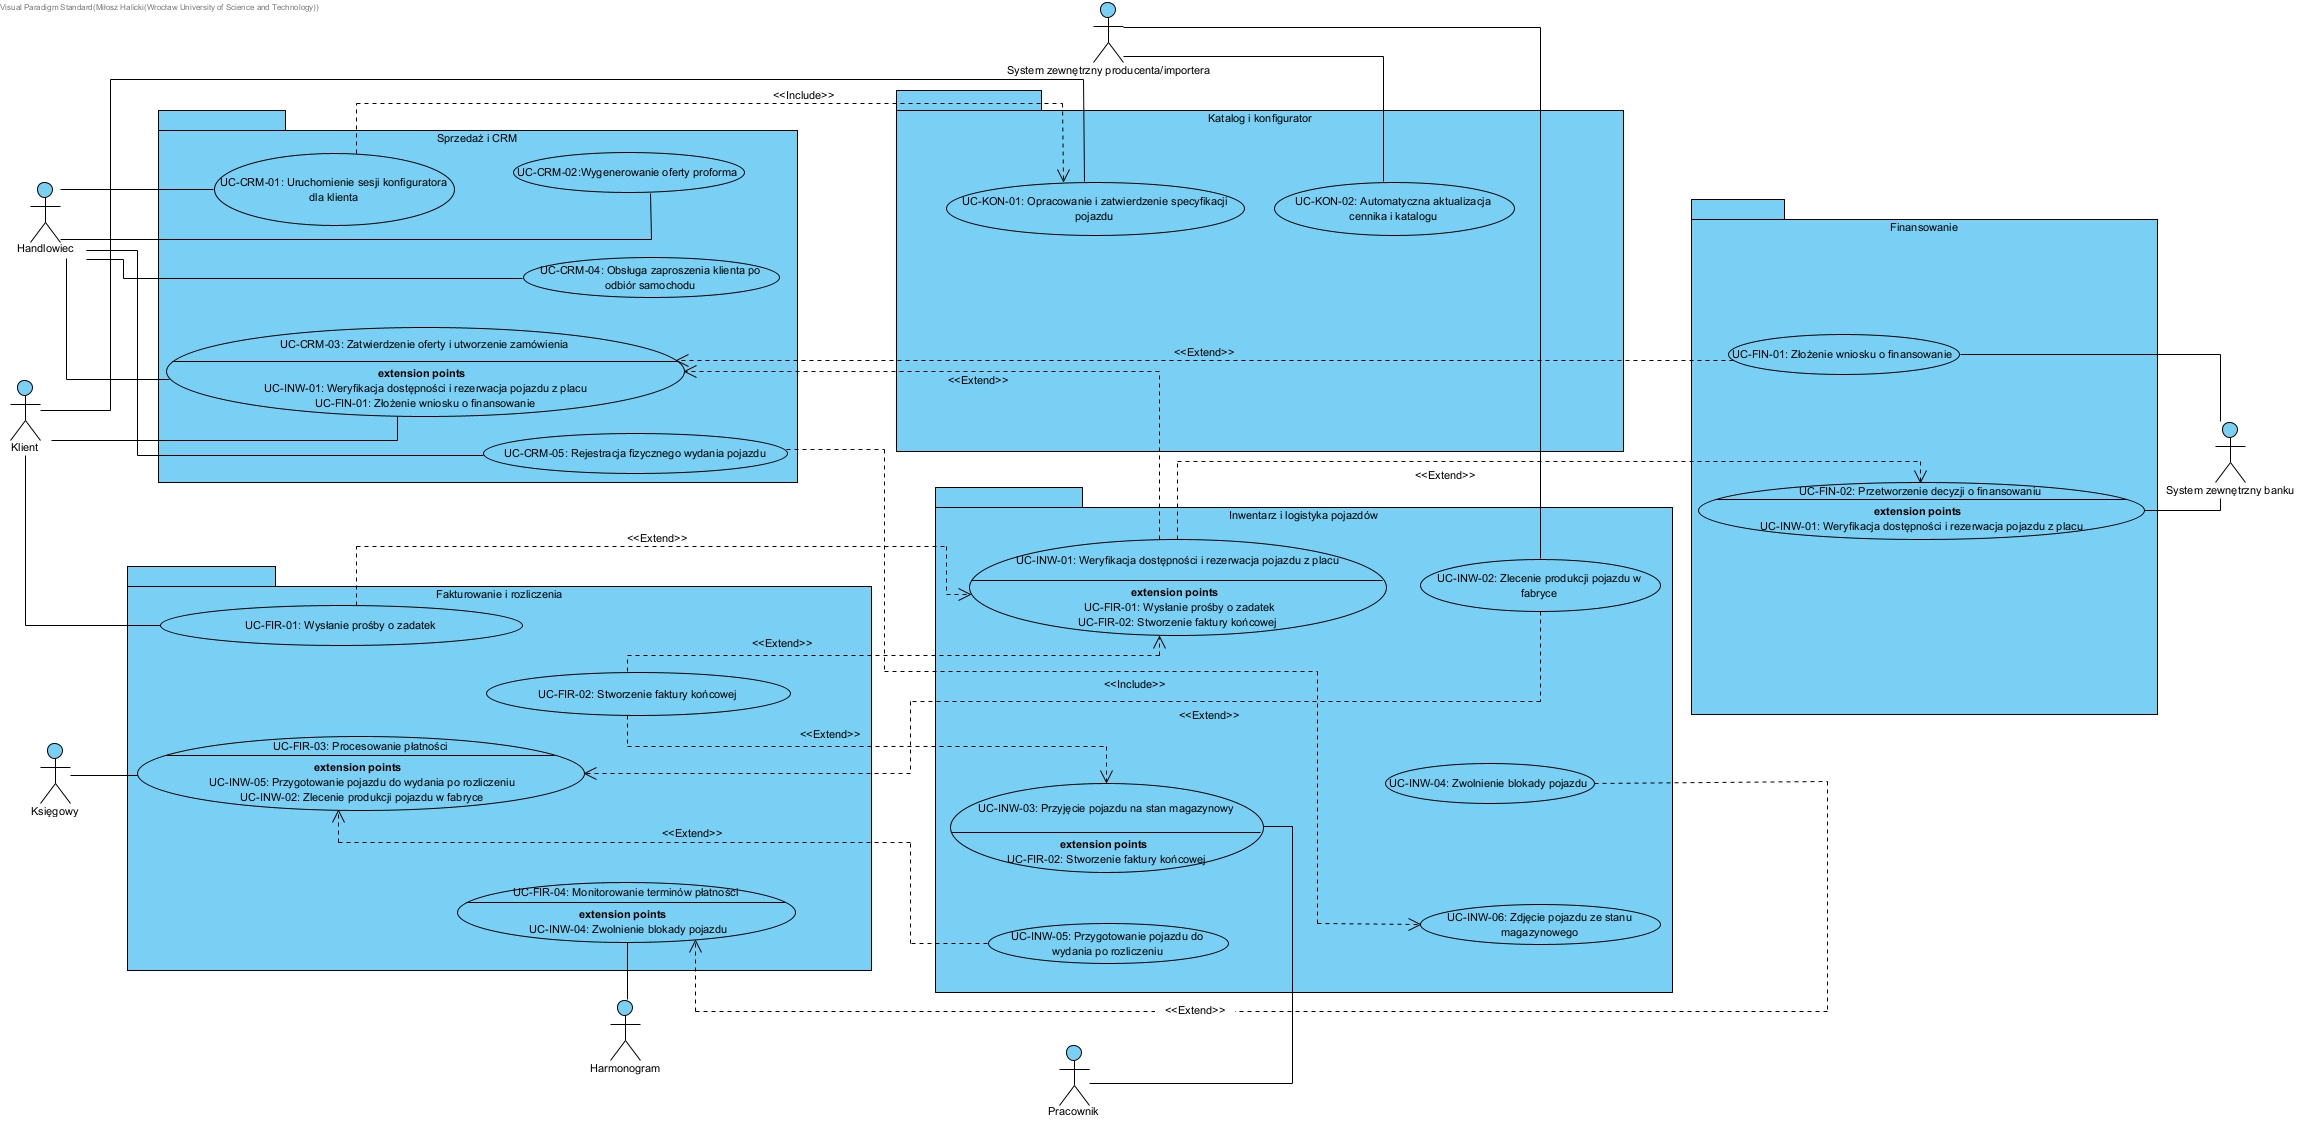
\includegraphics[width=\textwidth]{media/use-case-diagrams/Diagram przypadków użycia.jpg}
    \caption{Diagram przypadków użycia}
    \label{fig:hex_billing}
\end{figure}


% \subsection{Mapowanie kontekstów ograniczonych}

% Gorąca prośba do kierownika taktyki żeby to sobie kurwa zweryfikował bo ja nie wiem czy to jest ok a to jest jego zadanie ~ strateg
% \begin{figure}[H]
%     \centering
%     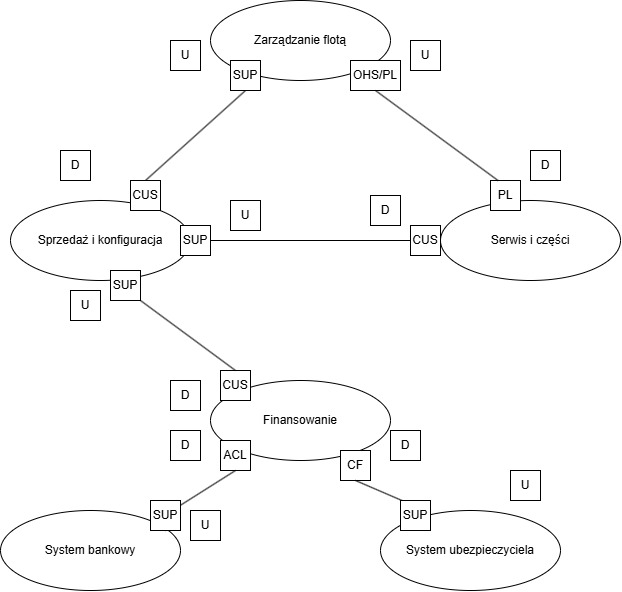
\includegraphics[width=0.8\textwidth]{media/ContextMapping.jpg}
%     \caption{Mapa kontekstów ograniczonych}
%     \label{fig:context-map}
% \end{figure}

% \begin{table}[H]
% \centering
% \caption{Mapowanie kontekstów}
% \label{tab:context-mapping}

% \renewcommand{\arraystretch}{1.2}
% \small

% \begin{tabular}{|p{3.2cm}|p{2.3cm}|p{2.3cm}|p{2.8cm}|p{4.2cm}|}
% \hline
% \textbf{Relacja} & \textbf{Upstream} & \textbf{Downstream} & \textbf{Wzorzec} & \textbf{Opis} \\
% \hline

% Flota $\rightarrow$ Sprzedaż &
% Flota &
% Sprzedaż &
% Customer-Supplier &
% Flota dostarcza dane o dostępności pojazdów dla sprzedaży. \\
% \hline

% Flota $\rightarrow$ Serwis &
% Flota &
% Serwis &
% Published Language &
% Flota publikuje zdarzenia logistyczne (VIN, status). \\
% \hline

% Sprzedaż $\rightarrow$ Serwis &
% Sprzedaż &
% Serwis &
% Customer-Supplier &
% Serwis przygotowuje pojazd zgodnie z zamówieniem. \\
% \hline

% Sprzedaż $\rightarrow$ Finansowanie &
% Sprzedaż &
% Finansowanie &
% Customer-Supplier &
% Finansowanie bazuje na danych z zamówienia. \\
% \hline

% Bank $\rightarrow$ Finansowanie &
% Bank &
% Finansowanie &
% ACL + Conformist &
% Finansowanie adaptuje zewnętrzny model banku przez ACL. \\
% \hline

% Ubezpieczyciel $\rightarrow$ Finansowanie &
% Ubezpieczyciel &
% Finansowanie &
% Conformist &
% System przyjmuje model ubezpieczyciela bez zmian. \\
% \hline

% \end{tabular}
% \end{table}

\newpage
\section{Architektura modelu}
\subsection{Kontekst Sprzedaży i CRM}
Kontekst Sprzedaży stanowi nadrzędny, główny obszar działalności biznesowej systemu. Zarządza on bezpośrednimi relacjami z klientem, kalkulacją ofertową oraz cyklem życia kontraktu sprzedażowego.

\subsubsection{Kanwa Kontekstu Sprzedaży}

\begin{figure}[H]
    \centering
    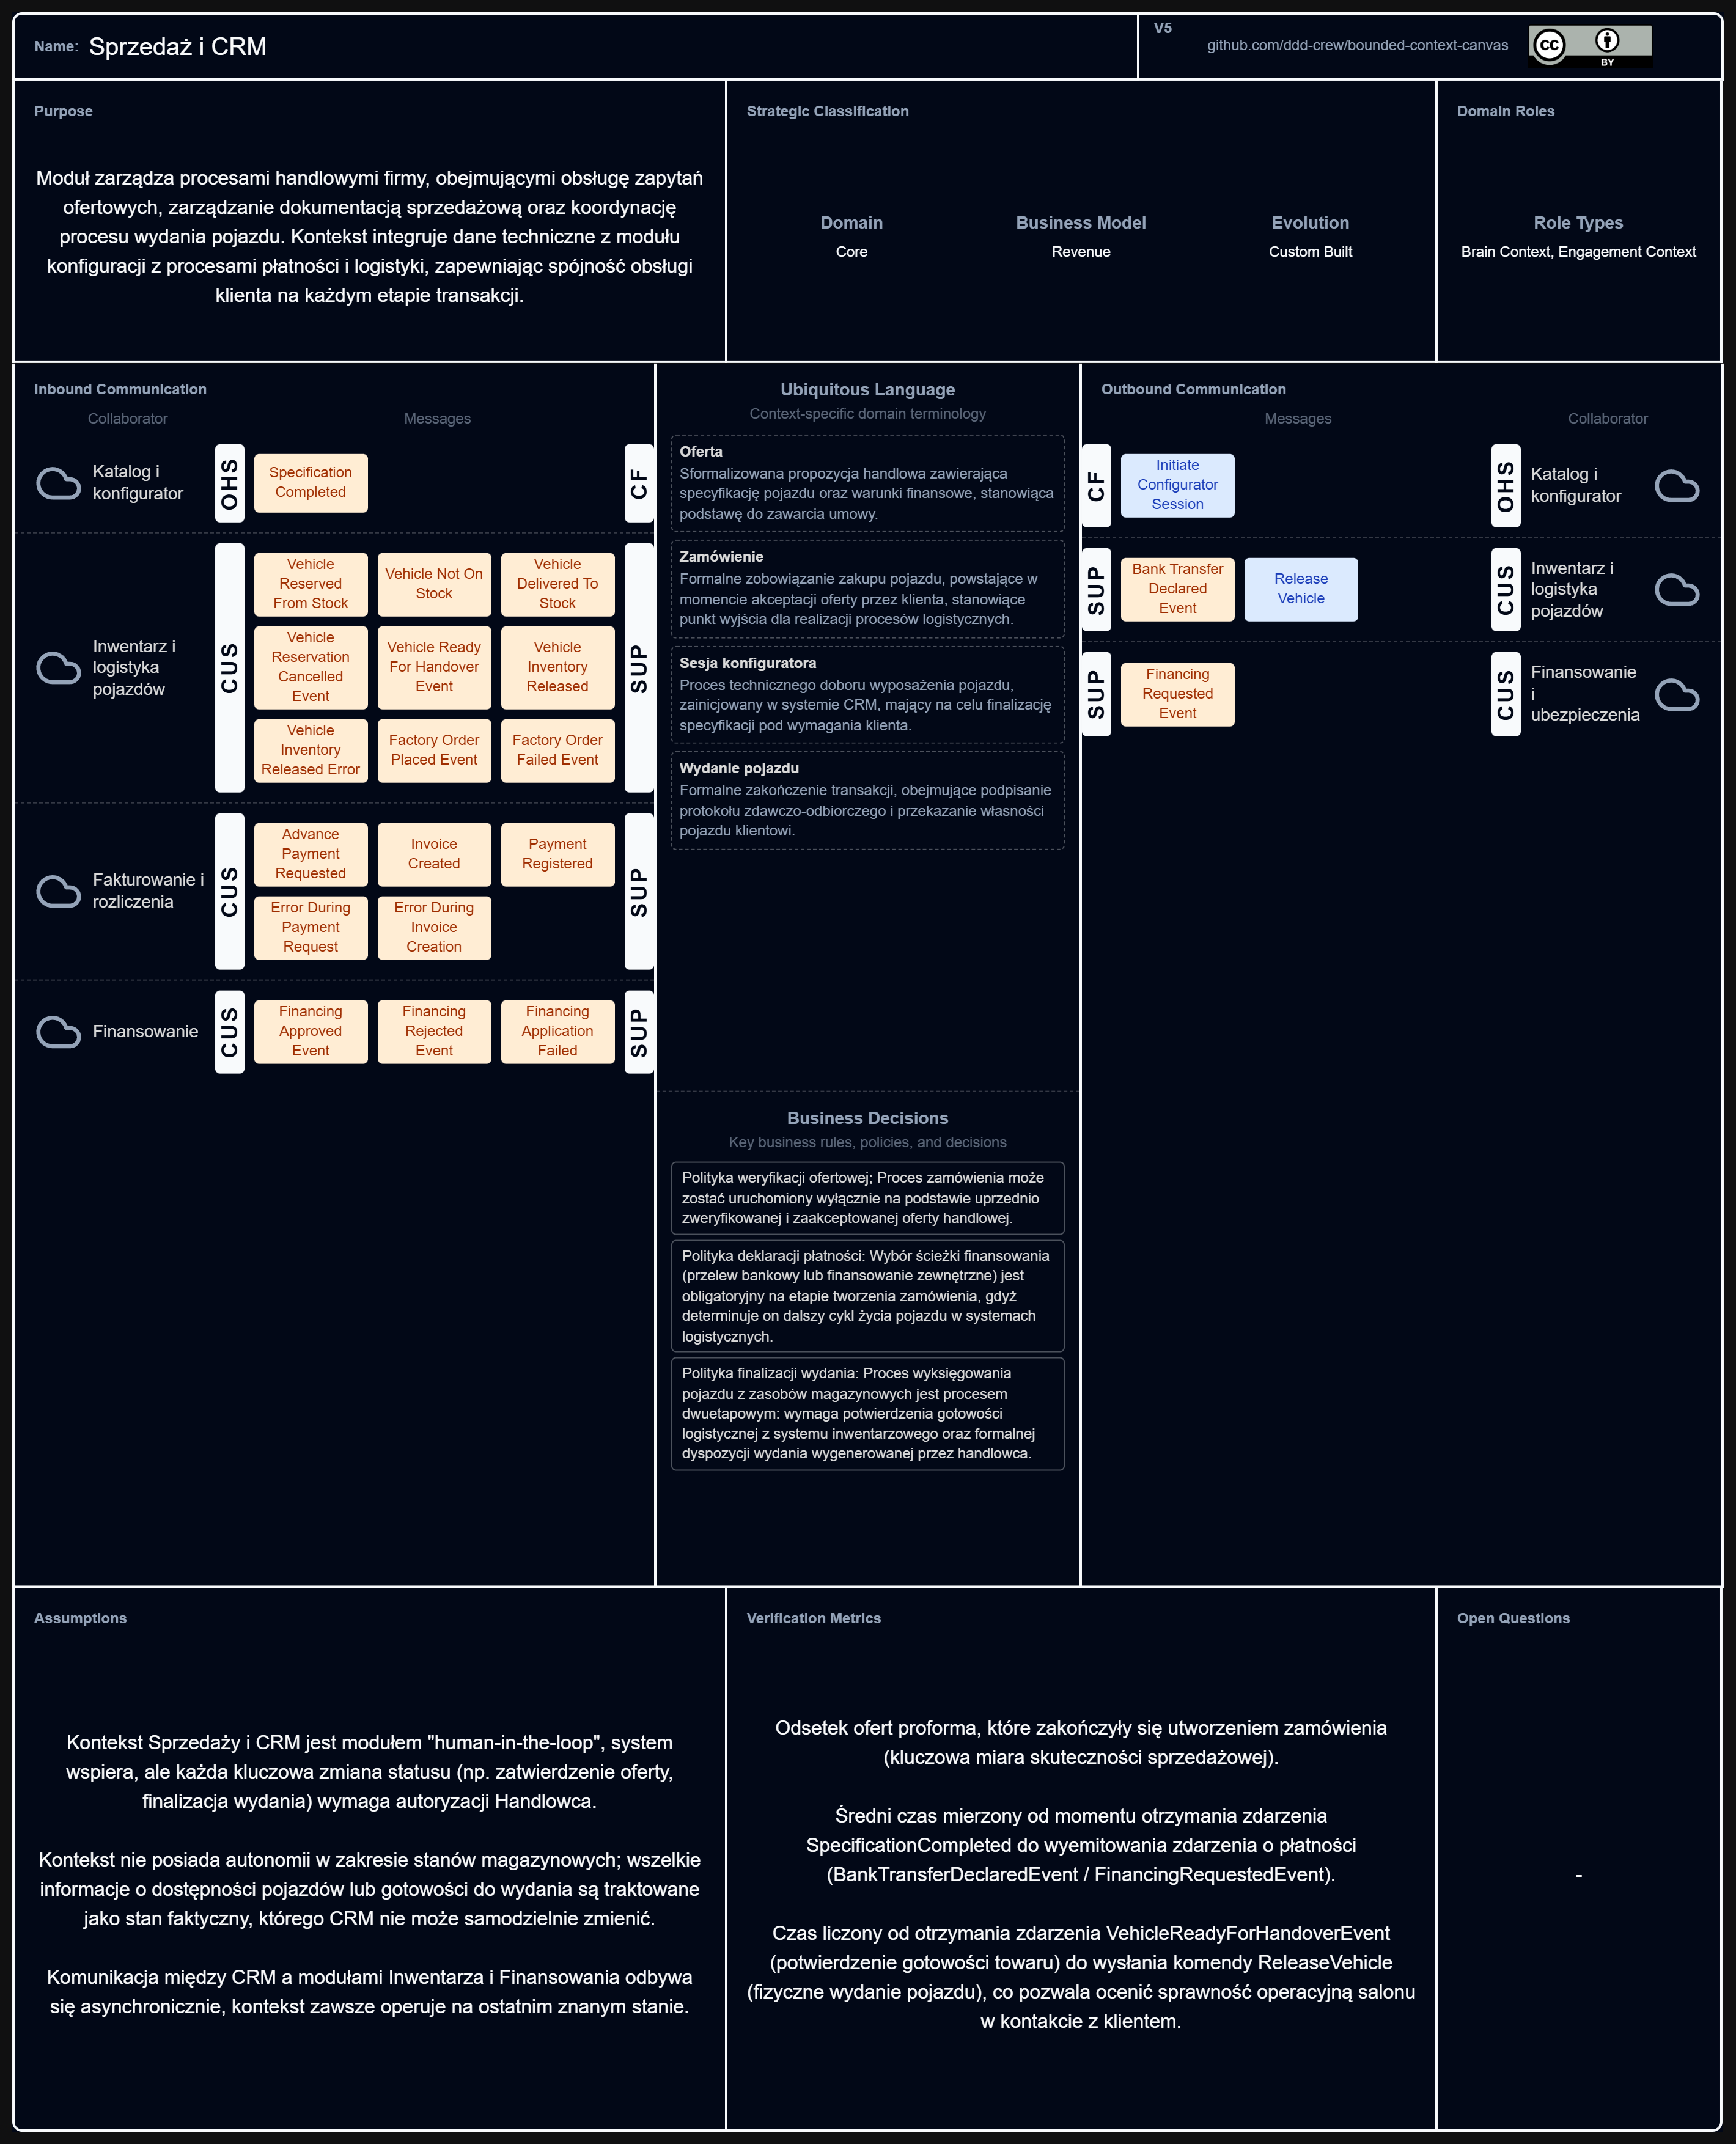
\includegraphics[width=\textwidth]{media/bounded-context-canvas/final/SIC_K1_TOTAL_FINAL.png}
    \caption{Kanwa Kontekstu Sprzedaży i CRM}
    \label{fig:hex_billing}
\end{figure}

\subsubsection{Przypadki użycia Kontekstu Sprzedaży}

% =====================================================
\textbf{UC-CRM-01: Uruchomienie sesji konfiguratora dla klienta}

\begin{longtable}{|p{4cm}|p{11cm}|}
\hline
\textbf{Element} & \textbf{Opis} \\
\hline

Identyfikator & UC-CRM-01 \\
\hline

Nazwa & Uruchomienie sesji konfiguratora dla klienta \\
\hline

Opis & 
Zainicjowanie procesu nowej sprzedaży poprzez wygenerowanie i otwarcie dedykowanej sesji w konfiguratorze pojazdów, przypisanej do konkretnego klienta i handlowca. \\
\hline

Aktor główny & Handlowiec \\
\hline

Aktorzy pomocniczy & - \\
\hline

Warunki wstępne & 
Klient wykazuje zainteresowanie zakupem nowego pojazdu. \\
\hline

Warunki końcowe & 
Wygenerowana zostaje nowa sesja, a kontekst emituje zdarzenie \textit{InitiateConfiguratorSession}. \\
\hline

Scenariusz główny & 
\begin{enumerate}
    \item Handlowiec wybiera opcję konfiguracji nowego pojazdu dla tego klienta.
    \item Kontekst emituje zdarzenie inicjujące \textit{InitiateConfiguratorSession}.
    \item System otwiera w nowym widoku interfejs konfiguratora (z modułu Katalogu).
\end{enumerate} \\
\hline

Scenariusze alternatywne & 
\begin{itemize}
    \item [] Brak.
\end{itemize} \\
\hline
\end{longtable}

\begin{figure}[H]
    \centering
    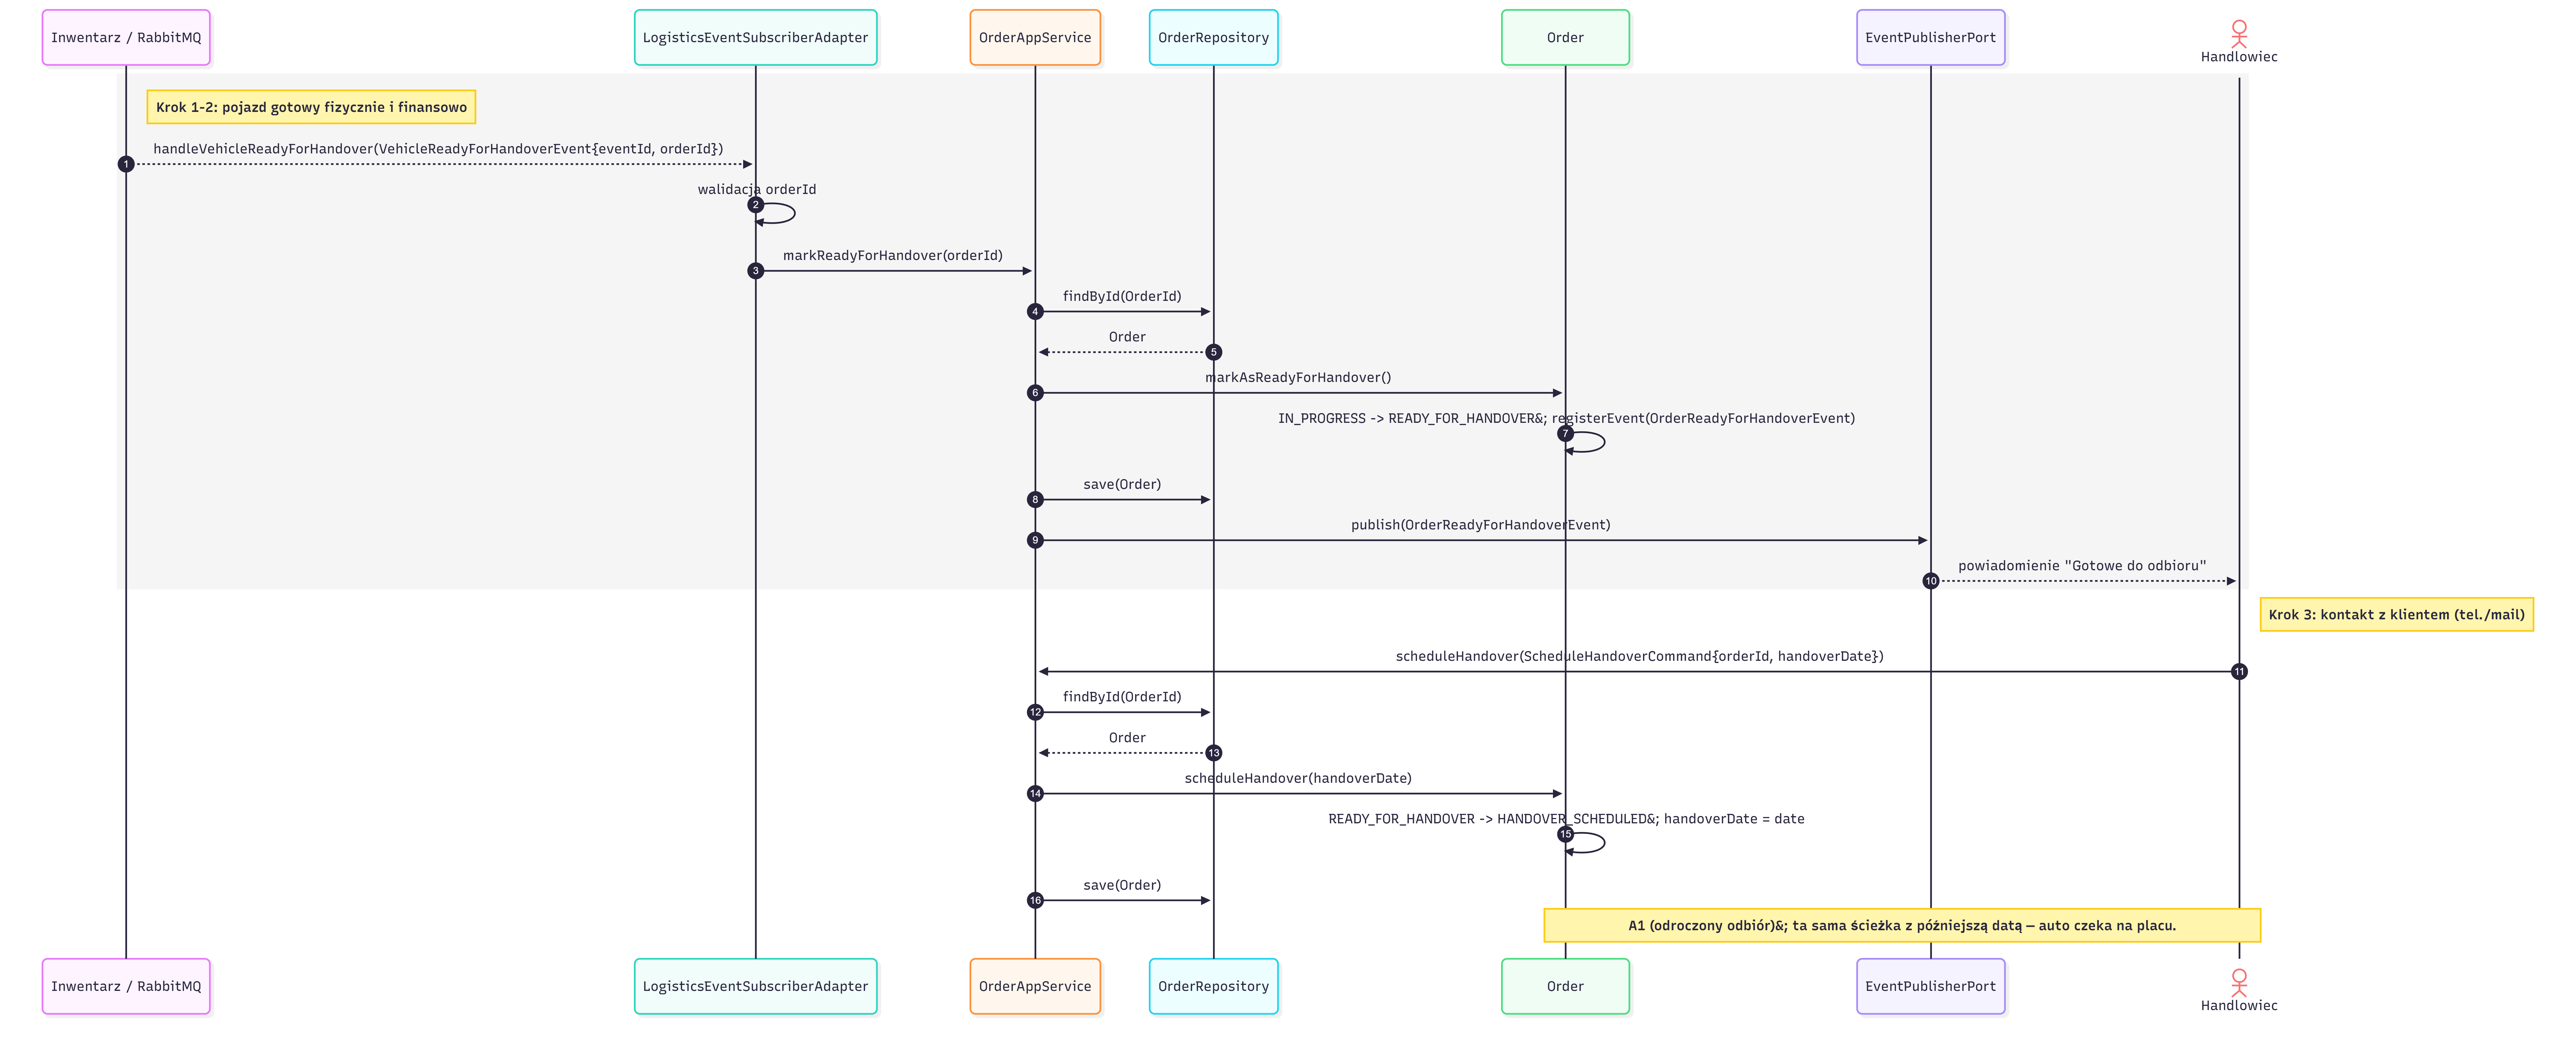
\includegraphics[width=1\textwidth]{media/diagramy_sekwencji/kontekst-sprzedazy/UC-CRM-01-Sekwencji.png}
    \caption{Diagram sekwencji dla przypadku użycia UC-CRM-01: Uruchomienie sesji konfiguratora dla klienta}
    \label{fig:seq_uc_crm_01}
\end{figure}

% =====================================================
\textbf{UC-CRM-02: Wygenerowanie oferty proforma}

\begin{longtable}{|p{4cm}|p{11cm}|}
\hline
\textbf{Element} & \textbf{Opis} \\
\hline

Identyfikator & UC-CRM-02 \\
\hline

Nazwa & Wygenerowanie oferty proforma \\
\hline

Opis & 
Proces utworzenia wstępnej oferty handlowej w systemie na podstawie danych (specyfikacji, ceny oraz danych kontaktowych klienta) otrzymanych od zdarzenia z konfiguratora. \\
\hline

Aktor główny & Handlowiec \\
\hline

Aktorzy pomocniczy & - \\
\hline

Warunki wstępne & 
Kontekst otrzymał zdarzenie \textit{SpecificationCompleted} zawierające pełną konfigurację, wyliczoną cenę oraz dane identyfikacyjne klienta. \\
\hline

Warunki końcowe & 
Nowa Oferta zostaje utworzona i zapisana w systemie ze statusem "W przygotowaniu". \\
\hline

Scenariusz główny & 
\begin{enumerate}
    \item System powiadamia handlowca o nowej specyfikacji oczekującej na ofertowanie.
    \item Handlowiec otwiera formularz nowej oferty.
    \item Handlowiec uzupełnia ofertę o dane klienta. Informacje o specyfikacji i cenie katalogowej uzupełniane są bezpośrednio z otrzymanego zdarzenia.
    \item Handlowiec generuje dokument oferty proforma zmieniając status na 'Utworzona' i prezentuje go klientowi.
\end{enumerate} \\
\hline

Scenariusze alternatywne & 
\begin{itemize}
    \item [] Brak.
\end{itemize} \\
\hline
\end{longtable}

\begin{figure}[H]
    \centering
    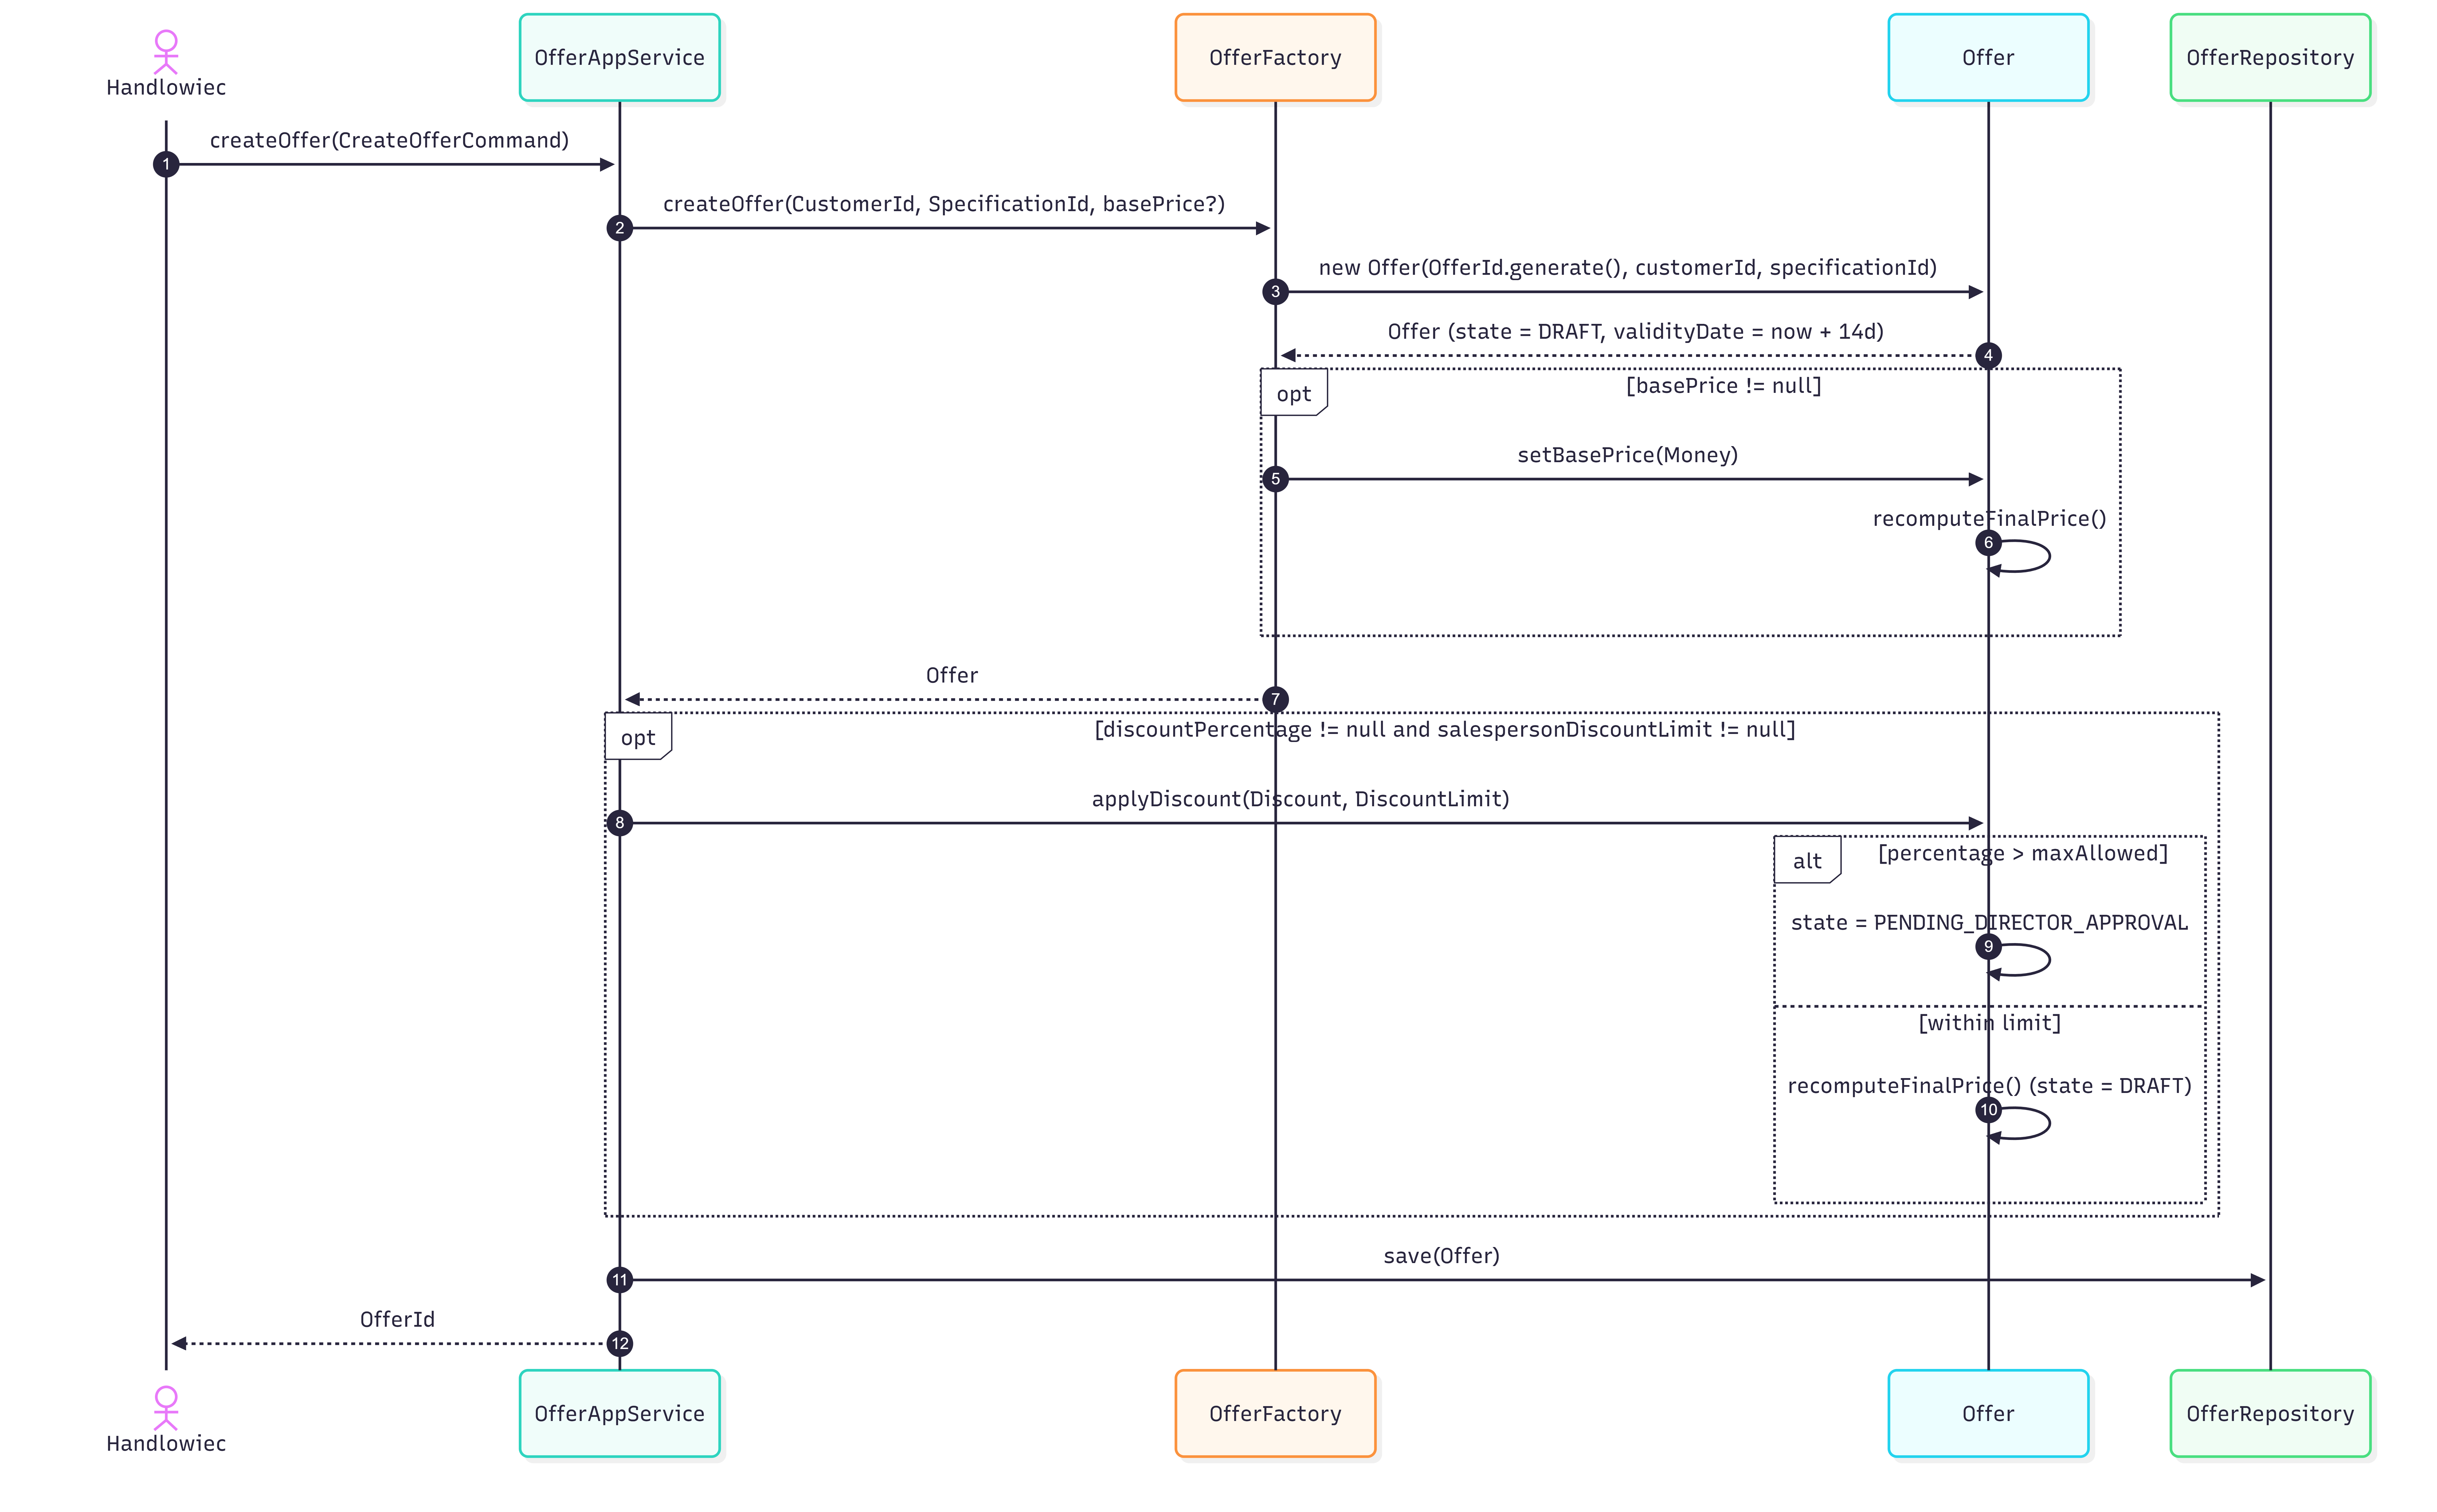
\includegraphics[width=1\textwidth]{media/diagramy_sekwencji/kontekst-sprzedazy/UC-CRM-02-Sekwencji.png}
    \caption{Diagram sekwencji dla przypadku użycia UC-CRM-02: Wygenerowanie oferty proforma}
    \label{fig:seq_uc_crm_02}
\end{figure}

% =====================================================
\textbf{UC-CRM-03: Zatwierdzenie oferty i utworzenie zamówienia}

\begin{longtable}{|p{4cm}|p{11cm}|}
\hline
\textbf{Element} & \textbf{Opis} \\
\hline

Identyfikator & UC-CRM-03 \\
\hline

Nazwa & Zatwierdzenie oferty, utworzenie zamówienia i wybór formy płatności \\
\hline

Opis & 
Proces akceptacji wygenerowanej oferty przez klienta oraz utworzenia na jej podstawie nowego zamówienia (osobnego agregatu), co uruchamia właściwe procesy logistyczne i sprzedażowe. \\
\hline

Aktor główny & Handlowiec \\
\hline

Aktorzy pomocniczy & Klient \\
\hline

Warunki wstępne & 
Wygenerowana i ważna oferta proforma (agregat Oferta) istnieje w systemie CRM. \\
\hline

Warunki końcowe & 
Oferta otrzymuje status "Zaakceptowana". W systemie powstaje nowe Zamówienie ze statusem "W realizacji", a system emituje odpowiednie zdarzenie inicjujące weryfikację stanu magazynowego placu lub proces bankowy. \\
\hline

Scenariusz główny & 
\begin{enumerate}
    \item Klient akceptuje warunki przedstawione na ofercie proforma.
    \item Handlowiec zmienia status oferty na "Zaakceptowana" w systemie CRM.
    \item Handlowiec tworzy nowe zamówienie na podstawie zaakceptowanej oferty.
    \item Handlowiec wprowadza na zamówieniu zadeklarowaną przez klienta formę płatności (Przelew lub Finansowanie).
    \item System CRM emituje zdarzenie \textit{BankTransferDeclaredEvent} (dla przelewu) LUB \textit{FinancingRequestedEvent} (dla finansowania).
\end{enumerate} \\
\hline

Scenariusze alternatywne & 
\begin{itemize}
    \item [A1] Klient odrzuca ofertę: W kroku 1 klient rezygnuje. Handlowiec zmienia status oferty na "Odrzucona". Nowe zamówienie nie powstaje, a żadne zdarzenie biznesowe nie jest emitowane do innych modułów.
\end{itemize} \\
\hline
\end{longtable}

\begin{figure}[H]
    \centering
    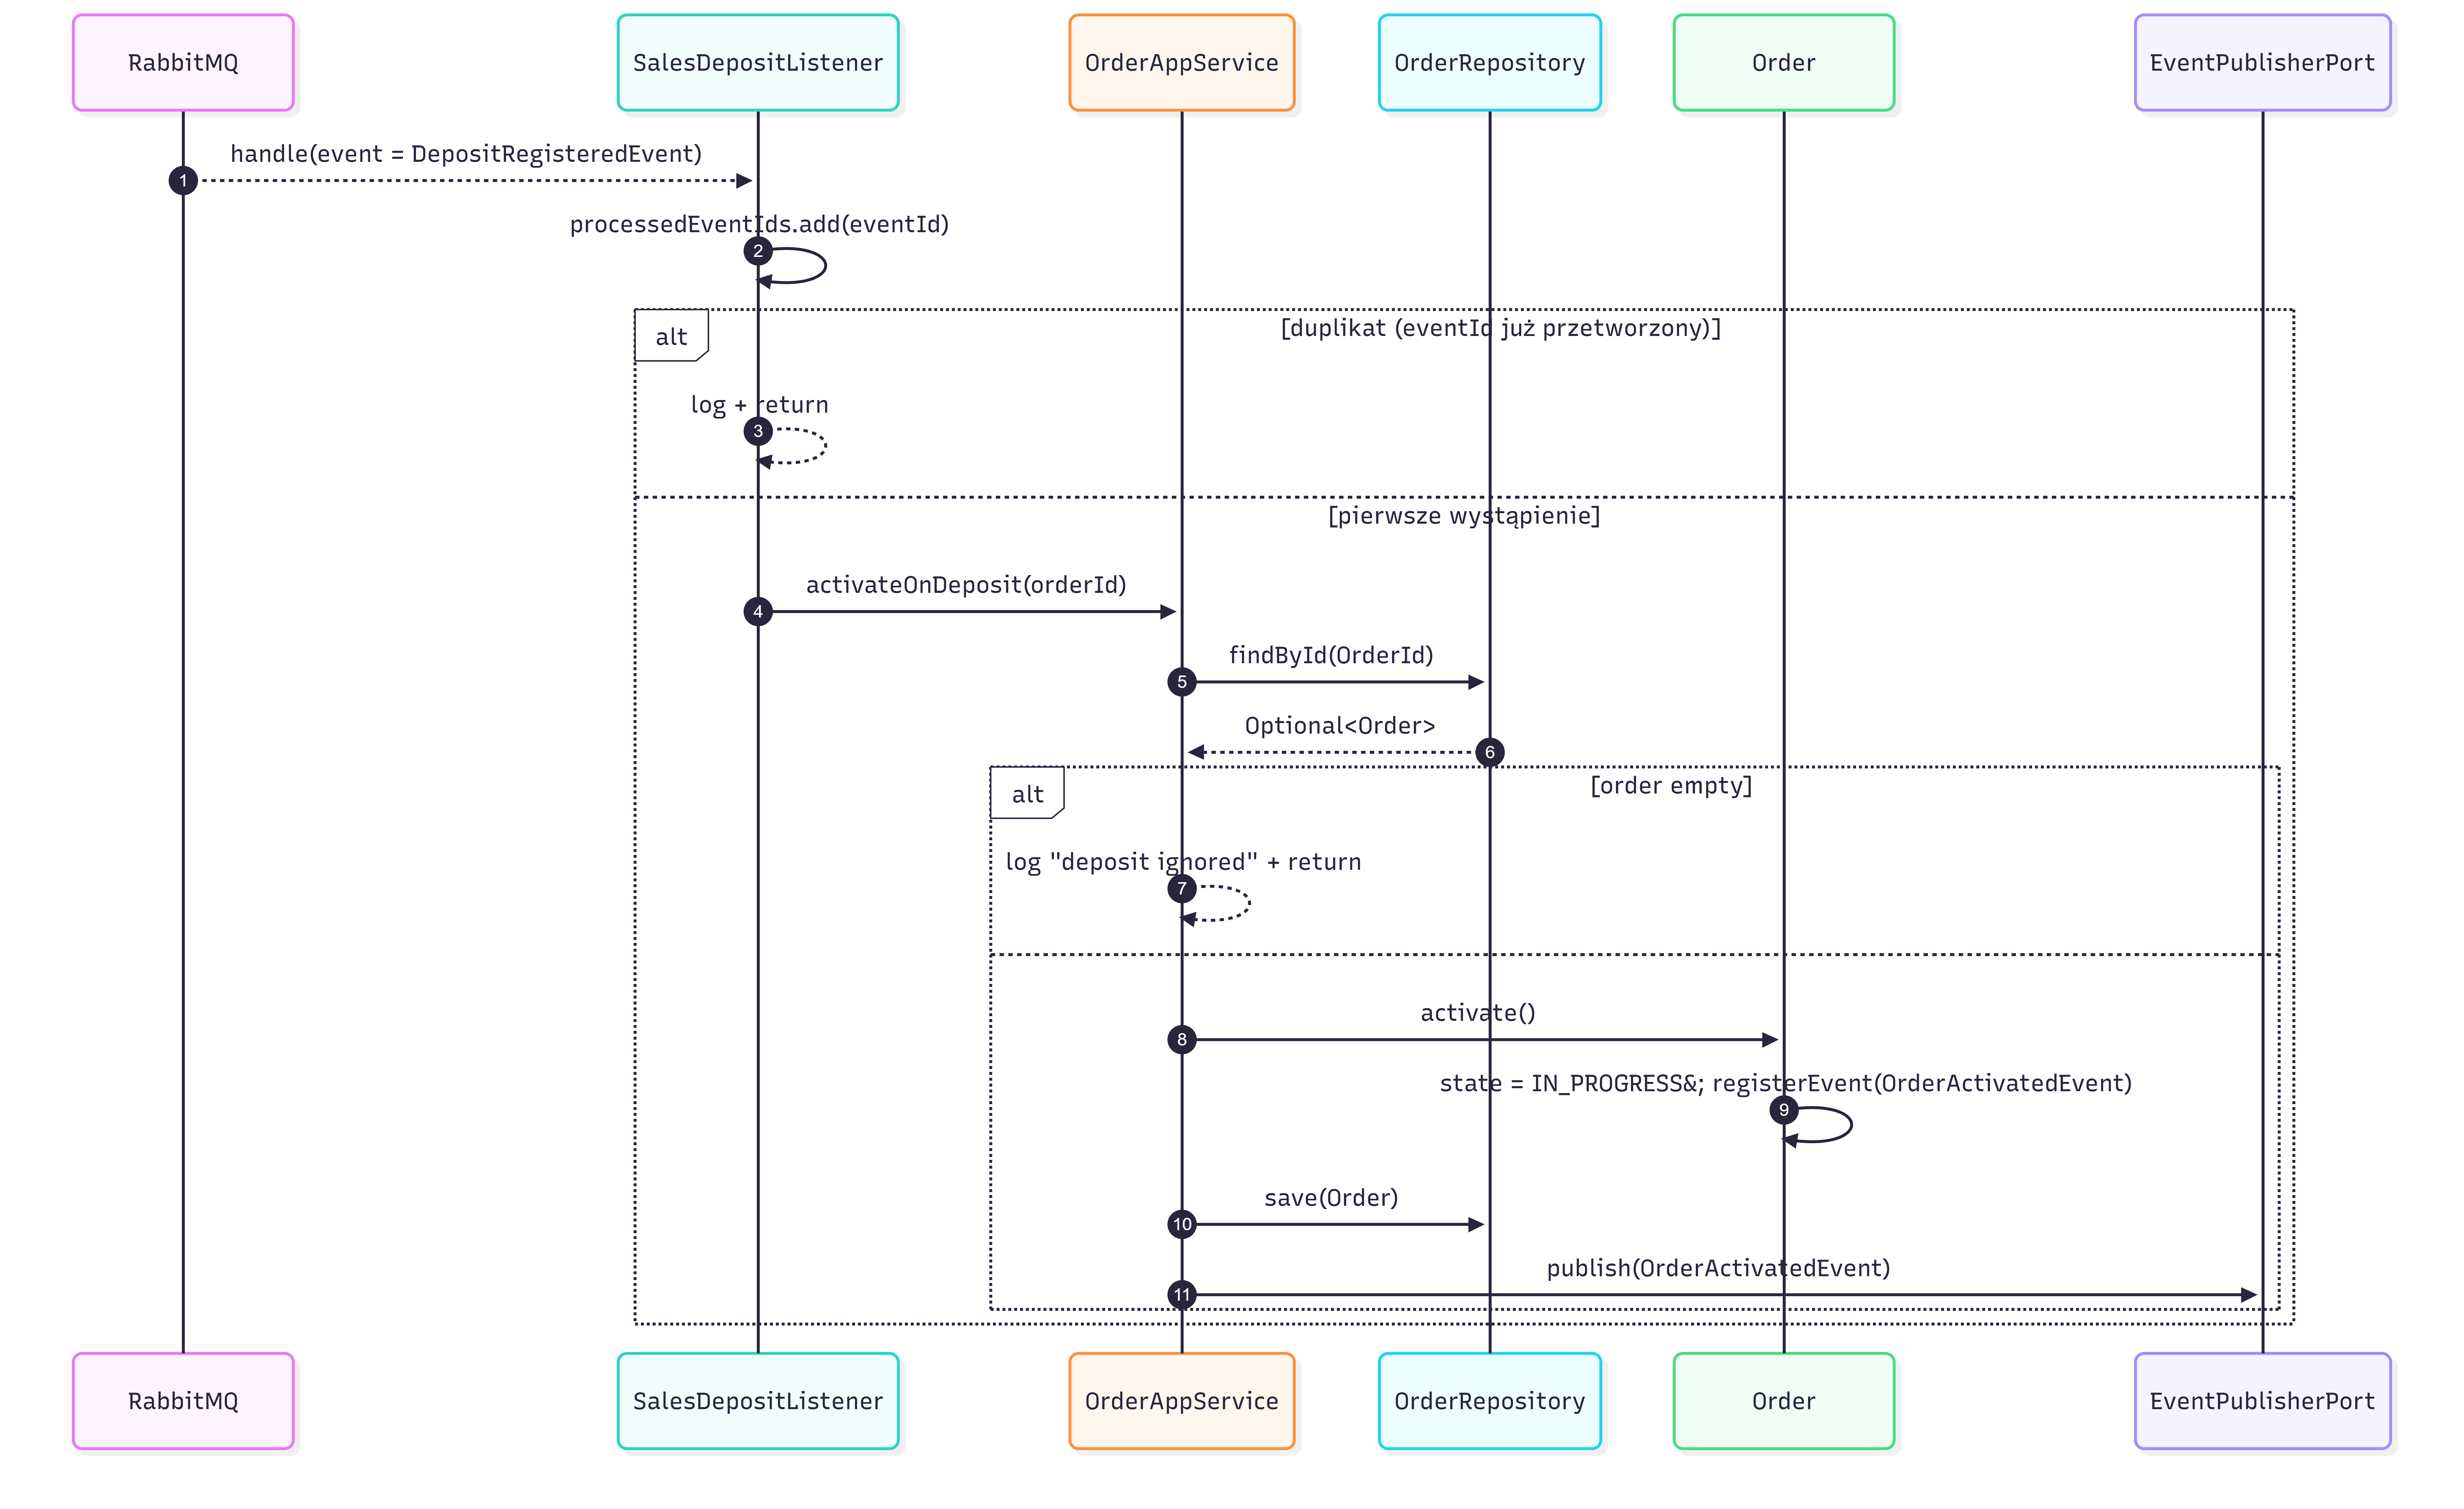
\includegraphics[width=1\textwidth]{media/diagramy_sekwencji/kontekst-sprzedazy/UC-CRM-03(cz2)-Sekwencji.png}
    \caption{Diagram sekwencji dla przypadku użycia UC-CRM-03 (cz.1): Konwersja oferty w zamówienie}
    \label{fig:seq_uc_crm_03cz1}
\end{figure}

\begin{figure}[H]
    \centering
    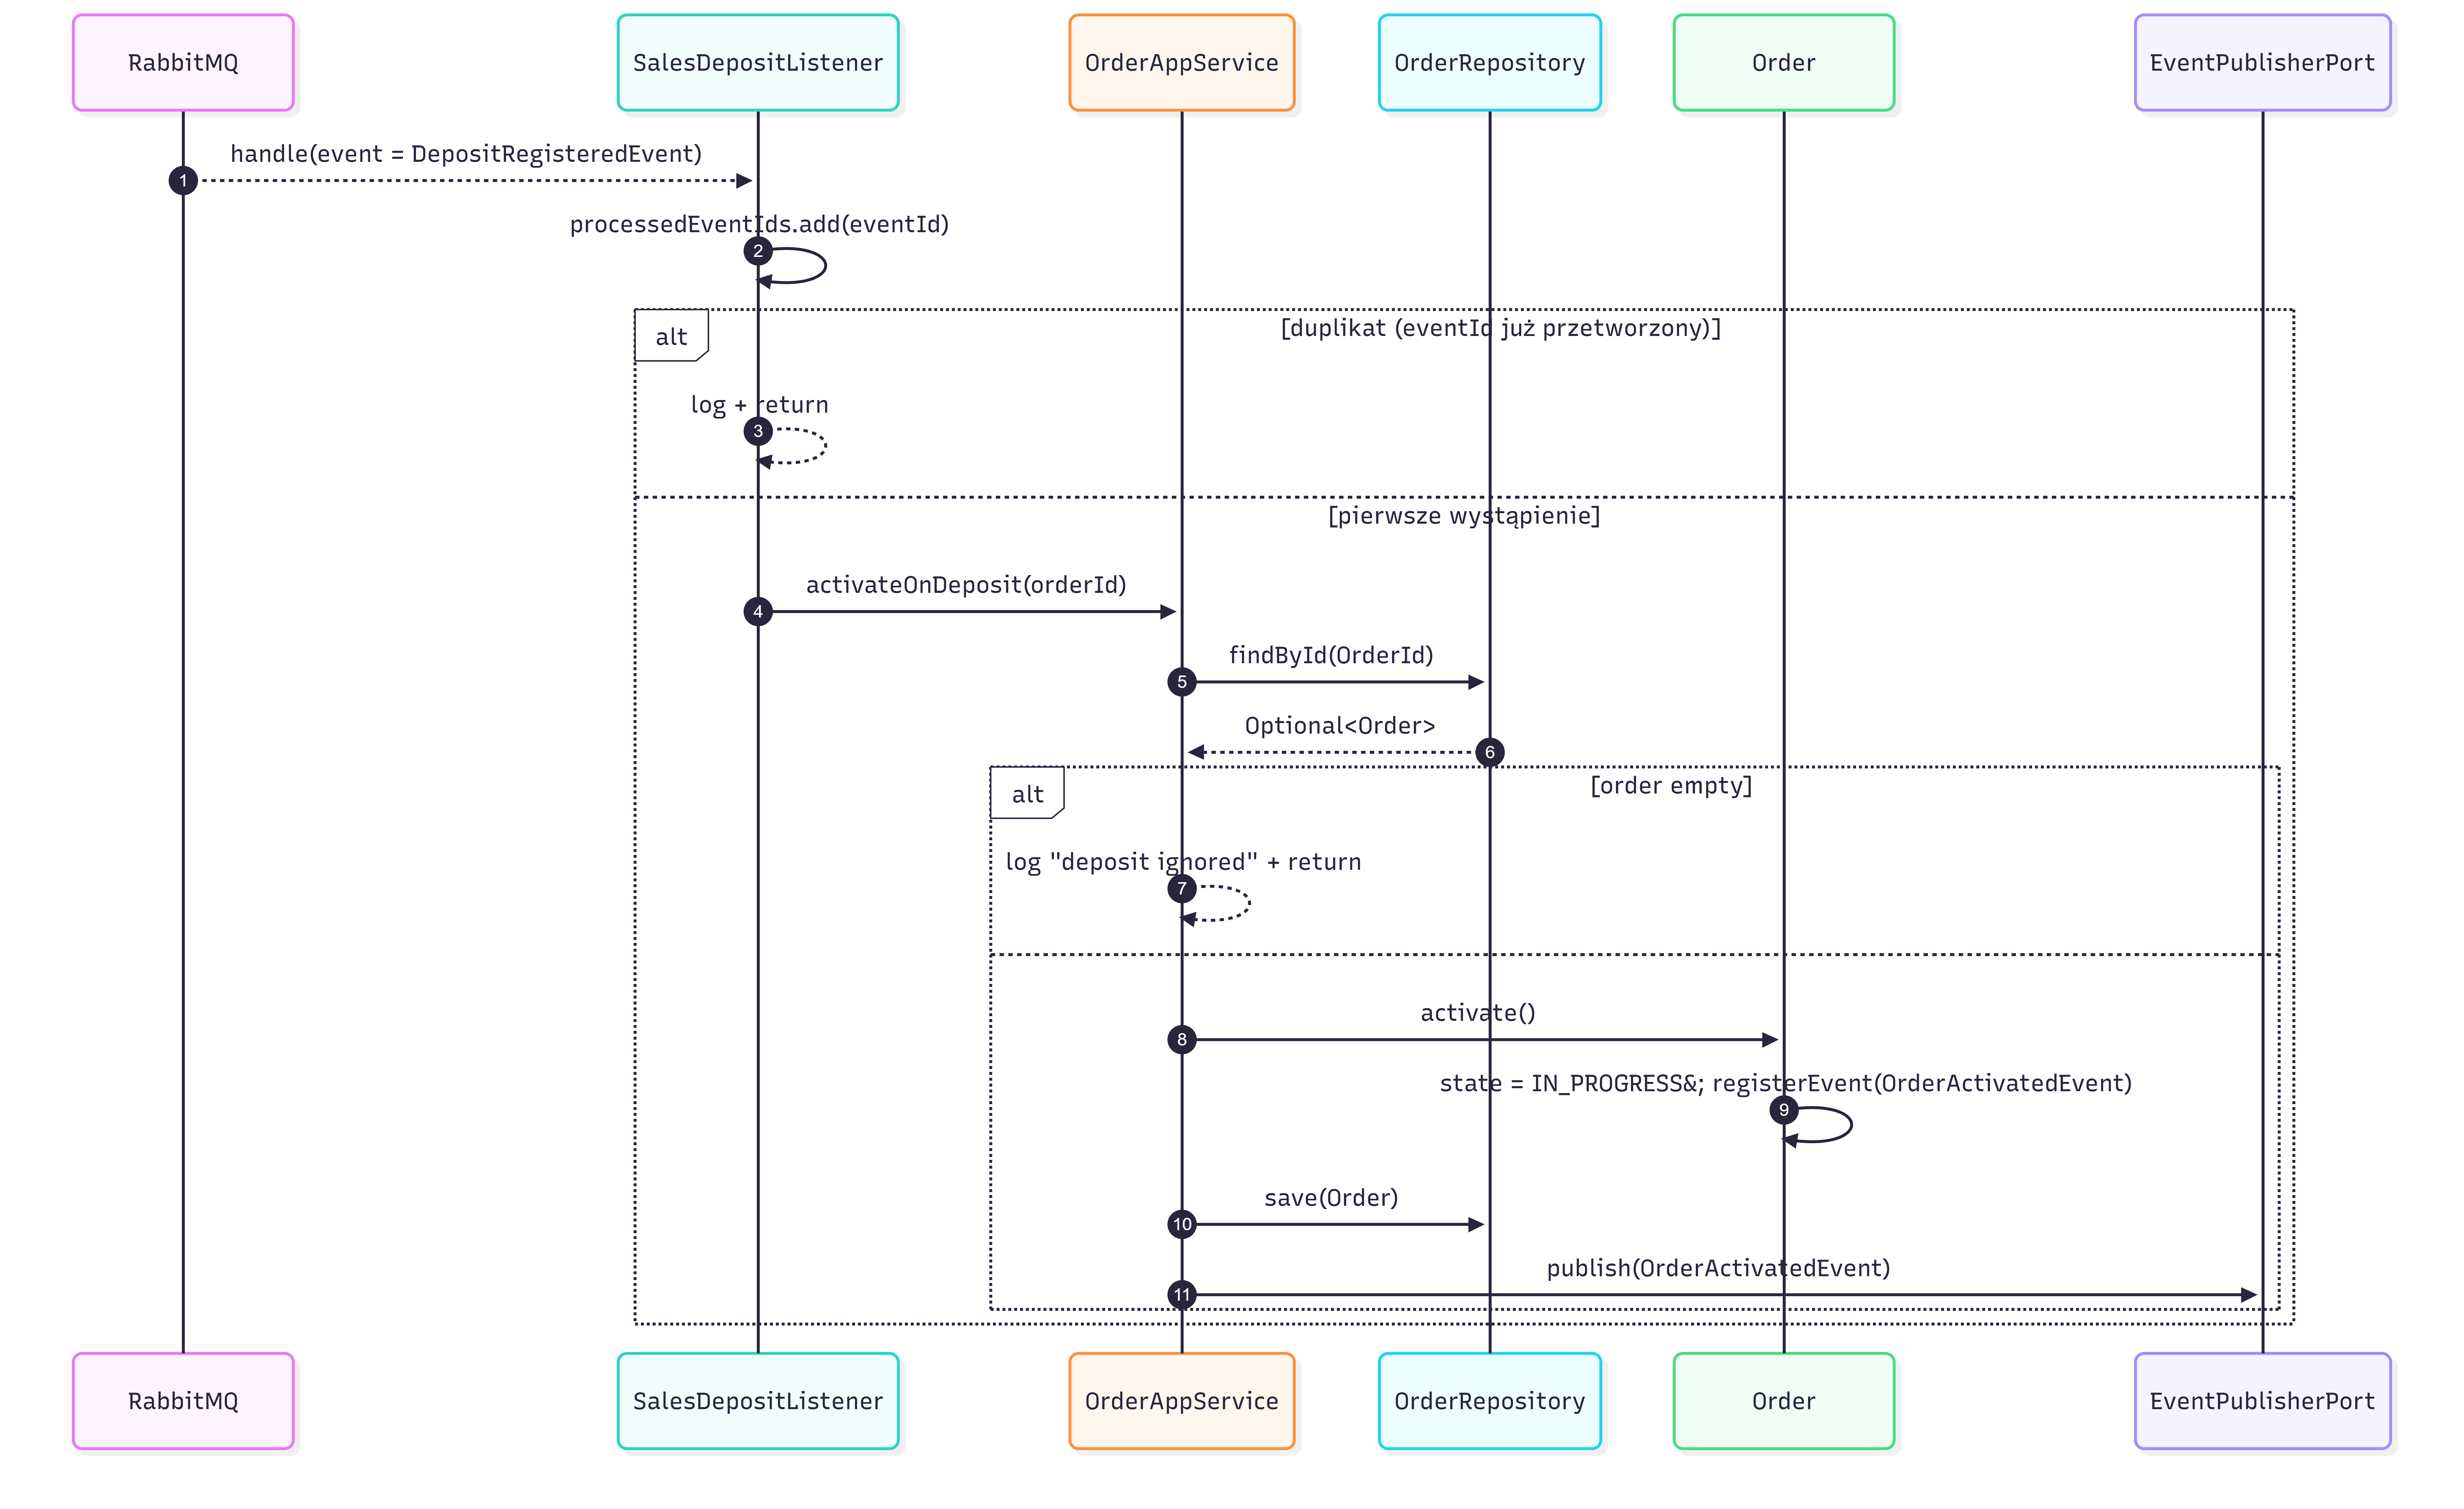
\includegraphics[width=1\textwidth]{media/diagramy_sekwencji/kontekst-sprzedazy/UC-CRM-03(cz2)-Sekwencji.png}
    \caption{Diagram sekwencji dla przypadku użycia  UC-CRM-03 (cz.2): Aktywacja po zadatku}
    \label{fig:seq_uc_crm_03cz2}
\end{figure}

% =====================================================
\textbf{UC-CRM-04: Obsługa zaproszenia klienta po odbiór}

\begin{longtable}{|p{4cm}|p{11cm}|}
\hline
\textbf{Element} & \textbf{Opis} \\
\hline

Identyfikator & UC-CRM-04 \\
\hline

Nazwa & Obsługa zaproszenia klienta po odbiór \\
\hline

Opis & 
Reakcja systemu na sygnał o pełnej gotowości fizycznej i finansowej pojazdu, uruchamiająca proces kontaktu z klientem w celu zaplanowania wydania auta. \\
\hline

Aktor główny & Handlowiec \\
\hline

Aktorzy pomocniczy & - \\
\hline

Warunki wstępne & 
Kontekst otrzymał zdarzenie \textit{VehicleReadyForHandoverEvent}. \\
\hline

Warunki końcowe & 
Ustalenie daty odbioru pojazdu i aktualizacja statusu zamówienia w CRM na "Umówiony na odbiór". \\
\hline

Scenariusz główny & 
\begin{enumerate}
    \item Kontekst sprzedaży i CRM odbiera zdarzenie \textit{VehicleReadyForHandoverEvent}.
    \item System zmienia status zamówienia na "Gotowe do odbioru" i generuje powiadomienie dla Handlowca.
    \item Handlowiec kontaktuje się z klientem (telefonicznie lub mailowo).
    \item Handlowiec wprowadza do systemu uzgodnioną z klientem datę i godzinę odbioru pojazdu.
    \item System aktualizuje status zamówienia na "Umówiony na odbiór".
\end{enumerate} \\
\hline

Scenariusze alternatywne & 
\begin{itemize}
    \item [A1] Odroczony odbiór: W kroku 3 klient informuje, że nie może odebrać auta w najbliższych dniach. Handlowiec ustawia odroczony termin w systemie, auto czeka na placu.
\end{itemize} \\
\hline
\end{longtable}

\begin{figure}[H]
    \centering
    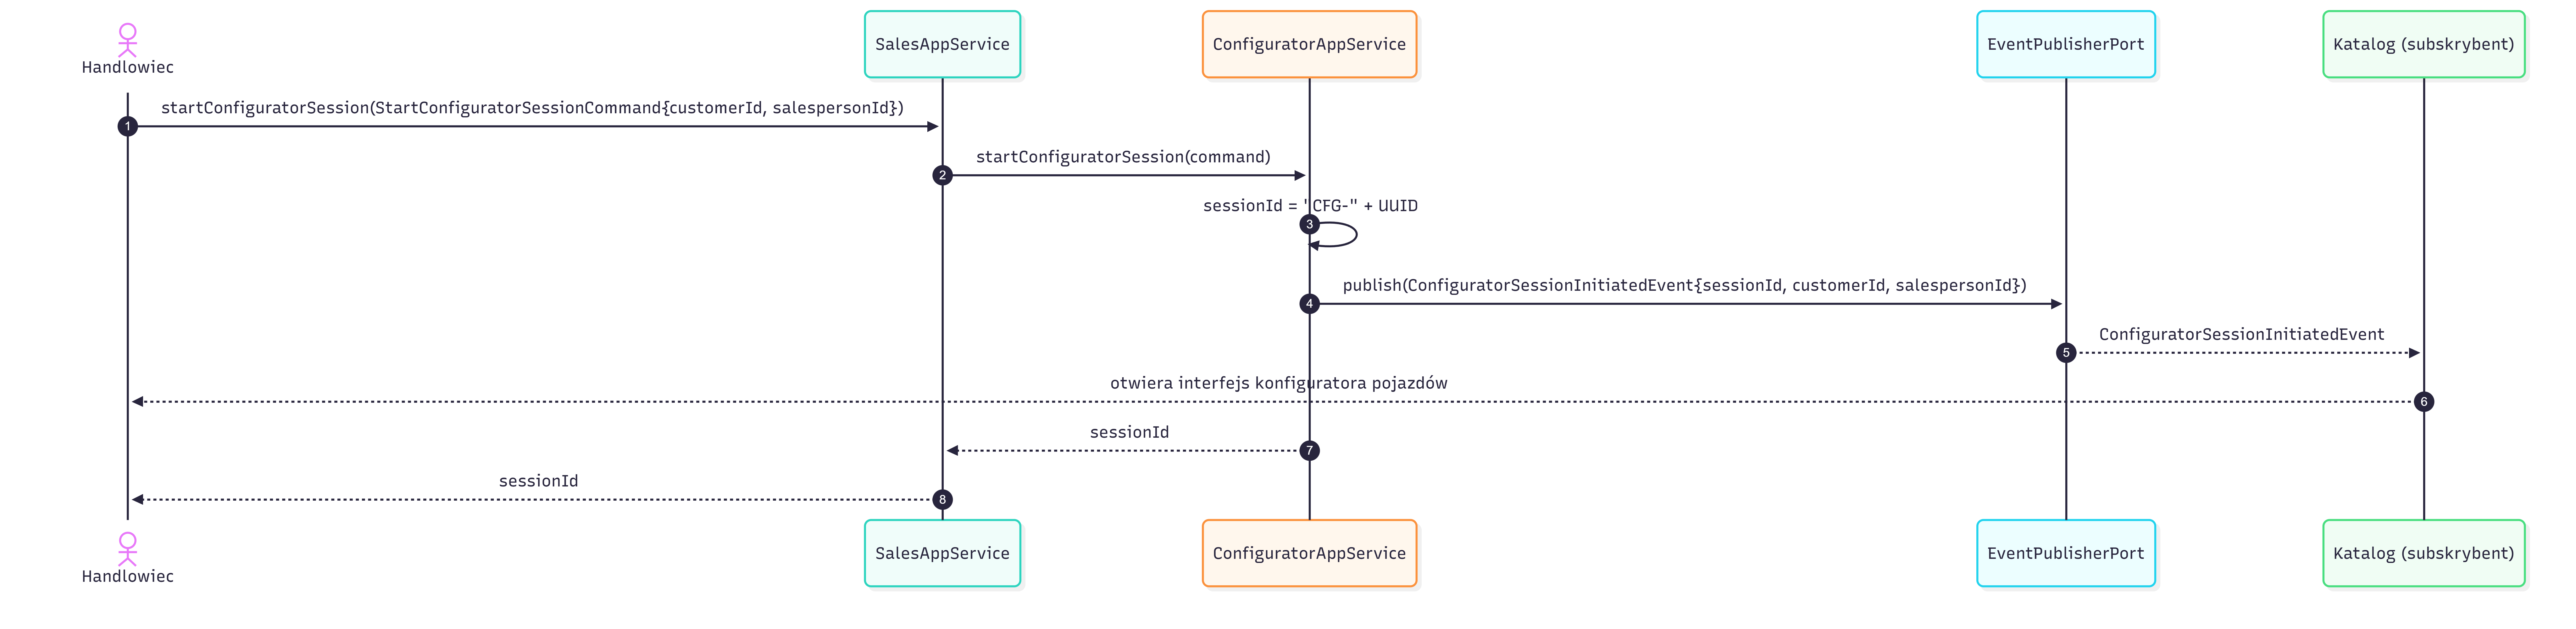
\includegraphics[width=1\textwidth]{media/diagramy_sekwencji/kontekst-sprzedazy/UC-CRM-04-Sekwencji.png}
    \caption{Diagram sekwencji dla przypadku użycia UC-CRM-04: Obsługa zaproszenia klienta po odbiór}
    \label{fig:seq_uc_crm_04}
\end{figure}

% =====================================================
\textbf{UC-CRM-05: Rejestracja fizycznego wydania pojazdu}

\begin{longtable}{|p{4cm}|p{11cm}|}
\hline
\textbf{Element} & \textbf{Opis} \\
\hline

Identyfikator & UC-CRM-05 \\
\hline

Nazwa & Rejestracja fizycznego wydania pojazdu \\
\hline

Opis & 
Finalny krok w procesie sprzedaży, zamykający transakcję i uruchamiający systemowe zwolnienie pojazdu. \\
\hline

Aktor główny & Handlowiec \\
\hline

Aktorzy pomocniczy & - \\
\hline

Warunki wstępne & 
Zamówienie posiada status "Umówiony na odbiór", klient stawił się w salonie. \\
\hline

Warunki końcowe & 
Zamówienie otrzymuje status "Zrealizowane", a CRM wysyła komendę \textit{ReleaseVehicle} do Inwentarza. \\
\hline

Scenariusz główny & 
\begin{enumerate}
    \item Handlowiec przeprowadza z klientem formalności papierowe i podpisuje protokół wydania.
    \item Handlowiec klika w systemie CRM przycisk potwierdzający wydanie pojazdu.
    \item Kontekst CRM wysyła komendę \textit{ReleaseVehicle} do modułu Inwentarza.
    \item System oznacza zamówienie jako 'Zrealizowane'.
\end{enumerate} \\
\hline

Scenariusze alternatywne & 
\begin{itemize}
    \item [A1] Odmowa Inwentarza: Po kroku 3 kontekst CRM odbiera z Inwentarza zdarzenie błędu \textit{VehicleInventoryReleasedError}. System wyświetla handlowcowi powiadomienie o blokadzie magazynowej i cofa zamówienie do statusu "Gotowe do odbioru".
\end{itemize} \\
\hline
\end{longtable}

\begin{figure}[H]
    \centering
    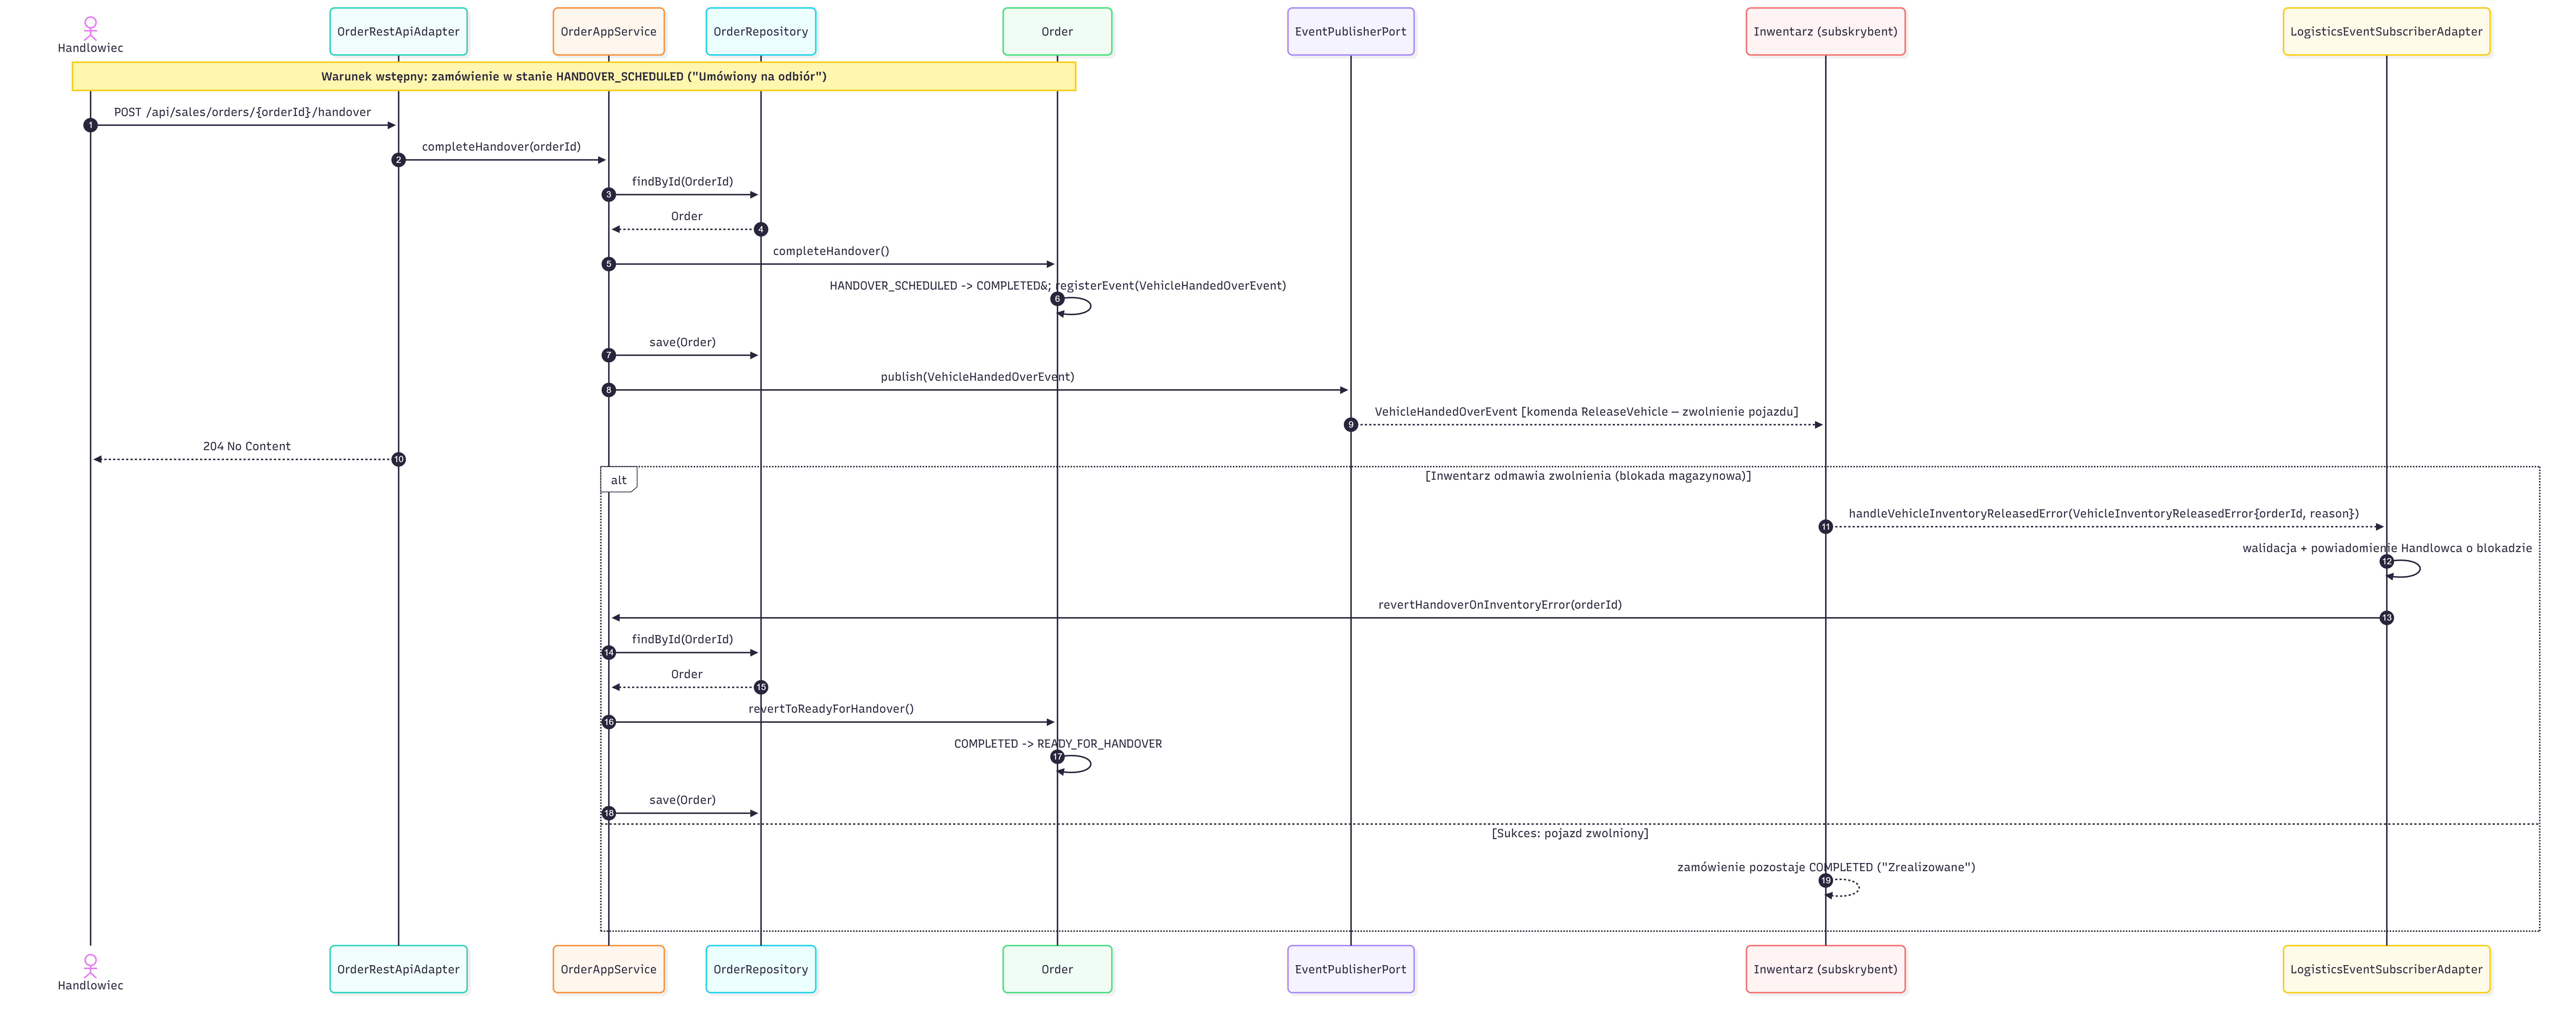
\includegraphics[width=1\textwidth]{media/diagramy_sekwencji/kontekst-sprzedazy/UC-CRM-05-Sekwencji.png}
    \caption{Diagram sekwencji dla przypadku użycia UC-CRM-05: Rejestracja fizycznego wydania pojazdu}
    \label{fig:seq_uc_crm_05}
\end{figure}

\subsubsection{Architektura Kontekstu Sprzedaży}

Kontekst Sprzedaży i CRM stanowi centralny węzeł operacyjny systemu, orkiestrujący pełen proces obsługi klienta – od inicjacji konfiguracji, aż po finalne wydanie pojazdu. Ze względu na wysoką złożoność biznesową i konieczność integracji z licznymi modułami zewnętrznymi, architekturę oparto na usłudze aplikacyjnej obsługi sprzedaży (\texttt{SalesService}), uzupełnionej o \texttt{ConfiguratorAppService} (sesje konfiguratora) i \texttt{SalesQueryService} (fasada zapytań), oraz na rygorystycznej dekompozycji logiki na trzy wyizolowane agregaty.

% MIEJSCE NA DIAGRAM ARCHITEKTURY (Sprzedaż Flowchart)
\begin{figure}[H]
    \centering
    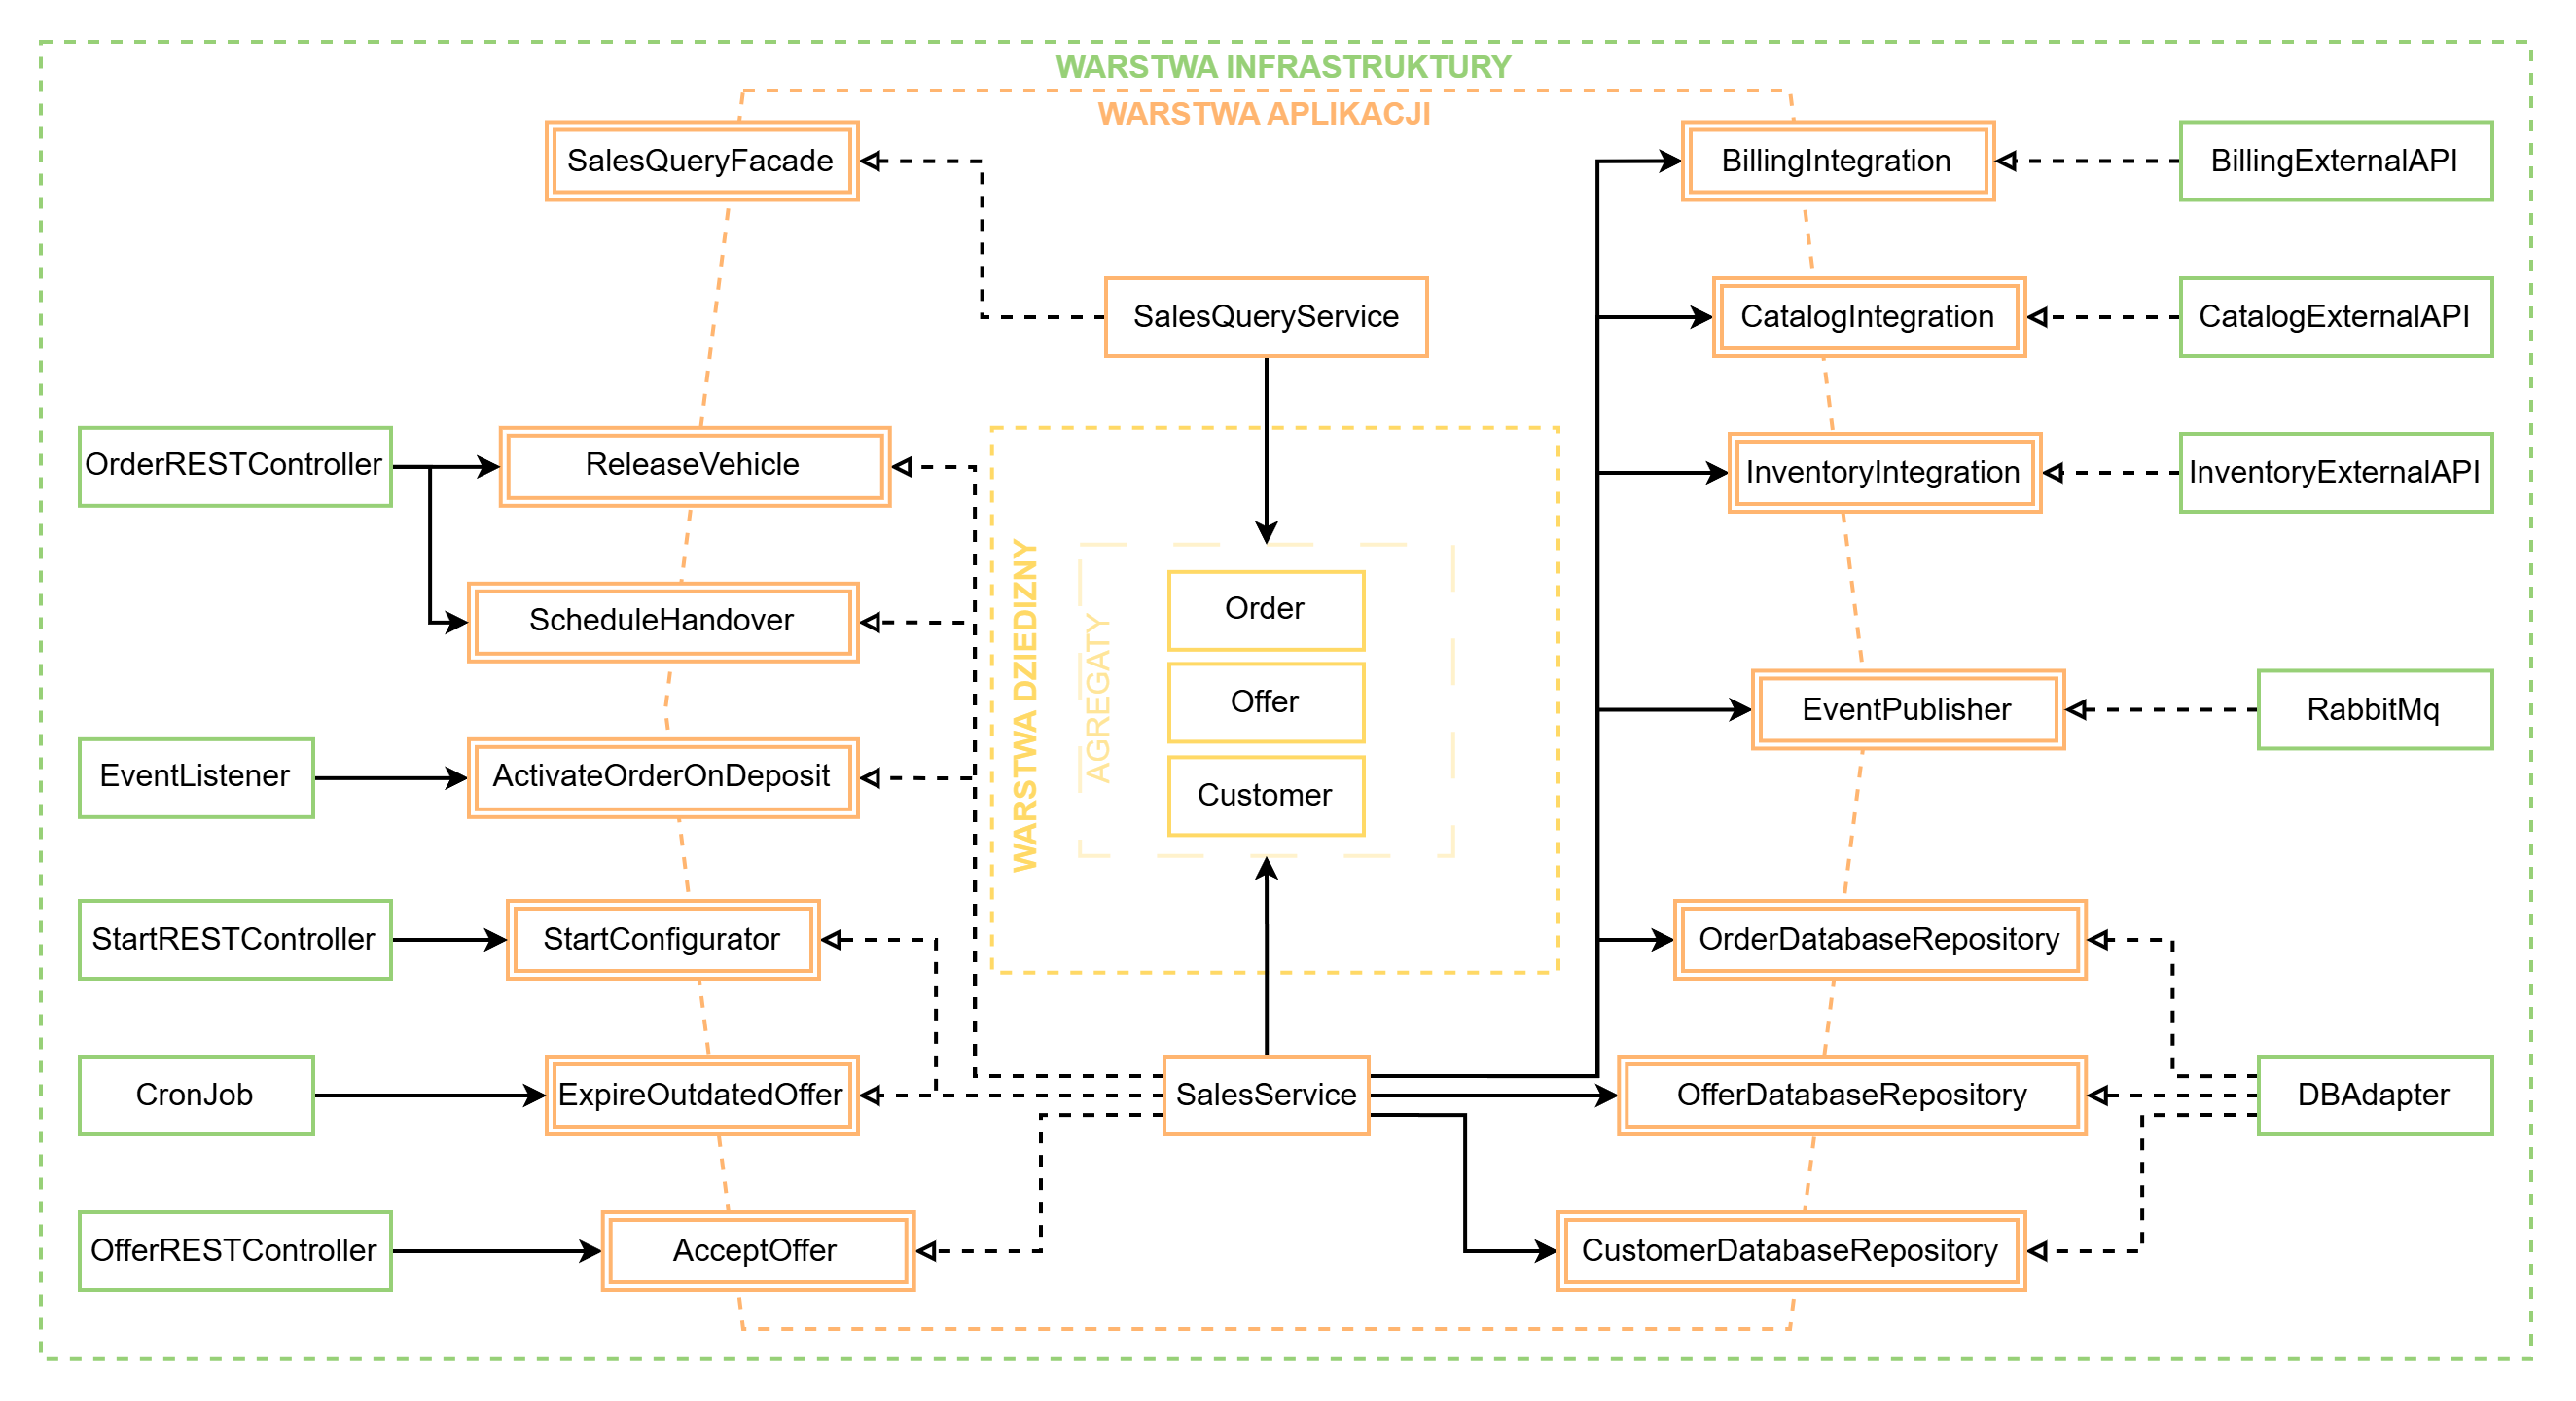
\includegraphics[width=\textwidth]{media/architektura_heksagonalna/SalesArchitecture.png}
    \caption{Architektura heksagonalna kontekstu sprzedaży i CRM}
    \label{fig:hex_sales}
\end{figure}

Poniżej przedstawiono szczegółowy opis interakcji pomiędzy warstwami, z podziałem na strony wejściową i wyjściową.

\paragraph{Strona Wejściowa: Porty i Adaptery} 
Ta strona heksagonu definiuje, w jaki sposób użytkownicy końcowi (klienci), handlowcy oraz inne moduły systemu inicjują procesy sprzedażowe.

\begin{itemize}
    \item \textbf{Inicjacja i Ofertowanie (Synchroniczne)}
    \begin{itemize}
        \item \textbf{Porty:} \texttt{StartConfigurator} (UC-CRM-01) oraz \texttt{ReceiveSpecificationUseCase} (UC-CRM-02). Interfejsy obsługujące bezstanowe otwarcie sesji konfiguratora oraz odbiór gotowej specyfikacji w celu wygenerowania wiążącej oferty.
        \item \textbf{Adaptery (HTTP):} \texttt{SessionRestApiAdapter} (sesje konfiguratora), \texttt{OfferRestApiAdapter} oraz \texttt{OrderRestApiAdapter}. Parsują żądania sieciowe z przeglądarki klienta na komendy domeny.
    \end{itemize}

    \item \textbf{Zarządzanie Transakcją i Wydaniem (Mieszane)}
    \begin{itemize}
        \item \textbf{Porty:} \texttt{AcceptOffer} (UC-CRM-03), \texttt{ActivateOrderOnDeposit} (aktywacja po wpłacie), \texttt{ScheduleHandover} (UC-CRM-04), \texttt{ReleaseVehicle} (UC-CRM-05) oraz \texttt{SynchronizeSpecificationPriceUseCase}. Interfejsy obsługujące konwersję oferty w zamówienie, koordynację wydań i zamknięcie procesu.
        \item \textbf{Adaptery:} Adaptery sieciowe (\texttt{OrderRestApiAdapter}, \texttt{InventoryWebhookRestAdapter}), adaptery nasłuchujące magistrali zdarzeń (\texttt{BillingEventSubscriberAdapter}, \texttt{CatalogEventSubscriberAdapter}, \texttt{LogisticsEventSubscriberAdapter}, \texttt{SalesDepositListener}) oraz \texttt{OfferExpirationCronJobAdapter} (cykliczne wygaszanie ofert). Adaptery zdarzeniowe reagują na sygnały z innych modułów (np. gotowość logistyczna z Inwentarza, zaksięgowanie wpłaty z Fakturowania), automatycznie wyzwalając odpowiednie porty.
    \end{itemize}
\end{itemize}

\paragraph{Strona Wyjściowa: Porty i Adaptery} 
Ta strona heksagonu definiuje zapotrzebowanie modułu Sprzedaży na utrwalanie wielowątkowego stanu biznesowego oraz komunikację z procesami logistyczno-finansowymi.

\begin{itemize}
    \item \textbf{Utrwalanie Stanu (Persystencja)}
    \begin{itemize}
        \item \textbf{Porty:} \texttt{CustomerDatabaseRepository}, \texttt{OfferDatabaseRepository} oraz \texttt{OrderDatabaseRepository}. Umożliwiają niezależny odczyt i zapis trzech głównych agregatów domeny.
        \item \textbf{Adaptery:} \texttt{OfferDatabaseAdapter} oraz \texttt{OrderDatabaseAdapter} — adaptery JPA (Hibernate; encje \texttt{OfferJpaEntity}/\texttt{OrderJpaEntity} i repozytoria Spring Data) z optymistyczną kontrolą współbieżności; \texttt{InMemoryCustomerRepository} — atrapa w pamięci dla klientów.
    \end{itemize}

    \item \textbf{Integracja Międzykontekstowa (Delegacja Zadań)}
    \begin{itemize}
        \item \textbf{Porty:} \texttt{InventoryIntegration}, \texttt{FinancingIntegrationPort}, \texttt{BillingIntegration}, \texttt{CatalogIntegration} oraz read-modele cen (\texttt{CatalogPriceQueryPort}, \texttt{SpecificationPriceReadModelPort}). Służą do koordynacji logistyki, finansowania i fakturowania oraz do lokalnego odczytu wyceny specyfikacji.
        \item \textbf{Adaptery:} \texttt{InventoryExternalApiAdapter}, \texttt{BillingExternalApiAdapter}, \texttt{CatalogExternalApiAdapter} (klienci HTTP z krótkim timeoutem), \texttt{FinancingEventBusAdapter} (zapytanie o zdolność przez publikację \texttt{FinancingRequestedEvent}), \texttt{InventoryCommandAdapter} oraz \texttt{InMemorySpecificationPriceReadModelAdapter}. Izolują jądro domeny od technicznych detali komunikacji z innymi kontekstami.
    \end{itemize}

    \item \textbf{Publikacja Zdarzeń}
    \begin{itemize}
        \item \textbf{Port:} \texttt{EventPublisher} (port Wspólnego Jądra). Interfejs zlecający emisję faktów biznesowych na zewnątrz modułu.
        \item \textbf{Adapter:} \texttt{SalesEventBusAdapter} (docelowo \texttt{RabbitMqEventPublisherAdapter} Wspólnego Jądra). Serializuje krytyczne zdarzenia dziedzinowe (np. \texttt{FinancingRequestedEvent}, \texttt{BankTransferDeclaredEvent}, \texttt{OrderPlacedEvent}) i umieszcza je na magistrali, umożliwiając modułom Fakturowania, Finansowania i Inwentarza asynchroniczną reakcję.
    \end{itemize}
\end{itemize}

\paragraph{Usługi Aplikacji}
W celu zapewnienia kontroli nad cyklem życia klienta zastosowano komplementarne komponenty koordynujące:
\begin{itemize}
    \item \textbf{SalesService} – główna usługa aplikacyjna orkiestrująca porty wejściowe sprzedaży (UC-CRM-02 do UC-CRM-05 oraz aktywacja po wpłacie). Pobiera agregaty (\texttt{Customer}, \texttt{Offer}, \texttt{Order}), wywołuje na nich dozwolone mutacje stanu, koordynuje porty integracyjne i utrwala wyniki w repozytoriach.
    \item \textbf{ConfiguratorAppService} – obsługa sesji konfiguratora (UC-CRM-01).
    \item \textbf{SalesQueryService} – realizacja publicznej fasady zapytań \texttt{SalesQueryFacade} (migawki nabywcy i oferty dla innych kontekstów).
\end{itemize}

\subsubsection{Agregaty Kontekstu Sprzedaży}

Cykl życia relacji handlowej został podzielony na dwa wyraźnie oddzielone od siebie etapy: niezobowiązujące negocjacje oraz prawnie wiążący kontrakt. Z uwagi na ich całkowicie odmienny cykl stanowy, zdekomponowano je na dwa niezależne agregaty.

% MIEJSCE NA DIAGRAM KLAS: Offer
\begin{figure}[h]
    \centering
    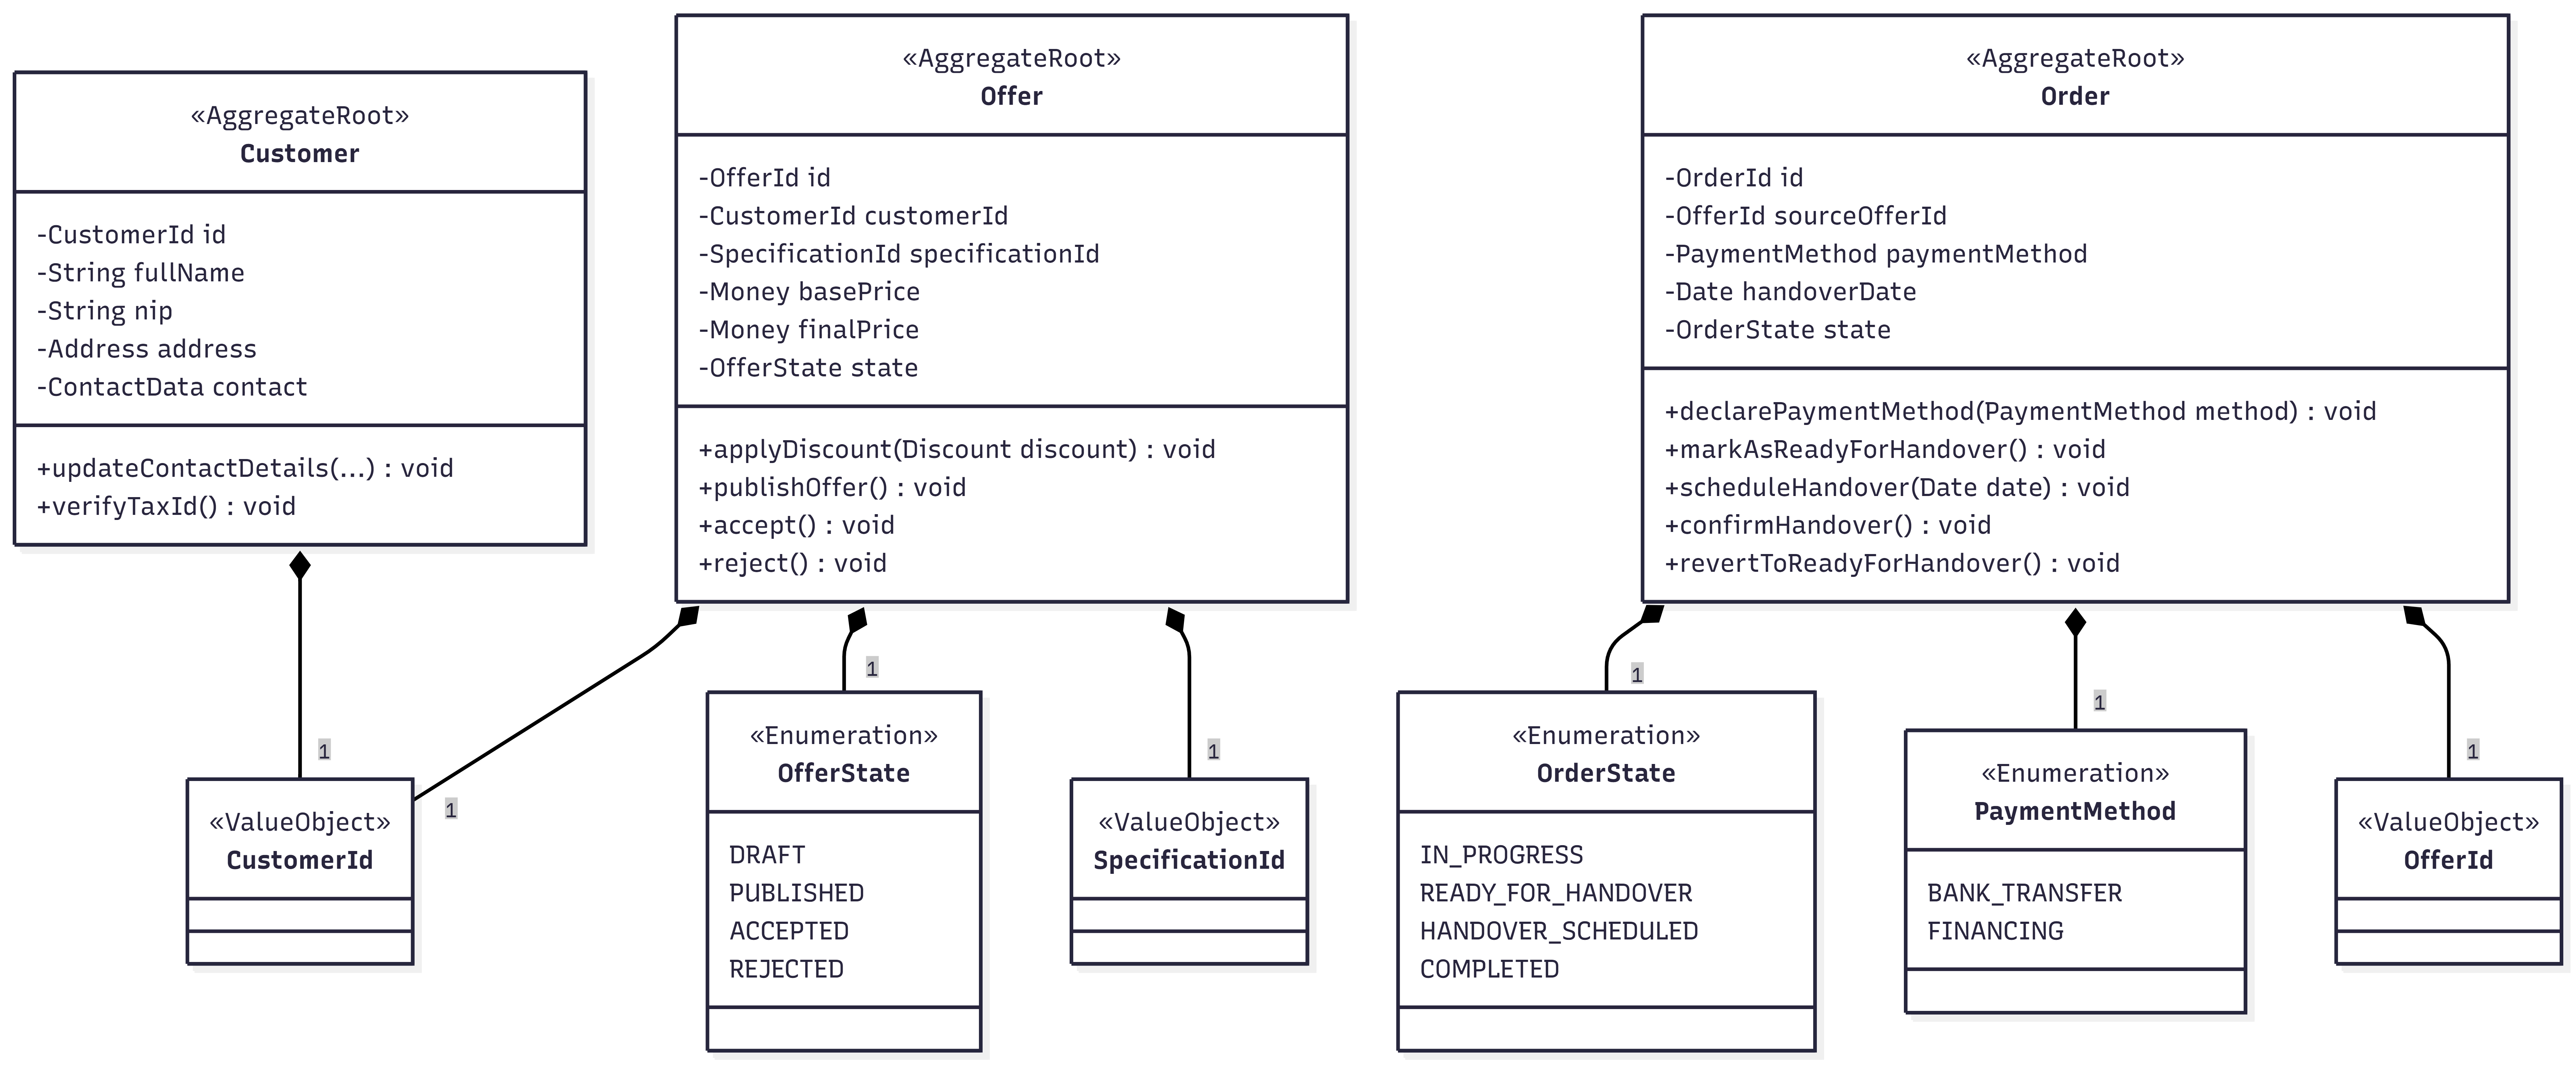
\includegraphics[width=\textwidth]{media/agregaty/kontekst-sprzedaży/customer-offer-order.png}
    \caption{Model strukturalny agregatu Oferty (Proforma).}
    \label{fig:agg_offer}
\end{figure}

Złożoność domeny CRM została opanowana poprzez ścisły podział odpowiedzialności pomiędzy trzy agregaty, które komunikują się ze sobą wyłącznie poprzez wzorzec referencji przez identyfikator.

\paragraph{Agregat: Klient (Customer)}
Stanowi rekord tożsamości klienta w systemie.
\begin{itemize}
    \item \textbf{Centralizacja Tożsamości:} Zamiast powielać dane osobowe w każdym dokumencie, agregat ten jest jedynym źródłem prawdy o kliencie. Pozostałe agregaty odwołują się do niego wyłącznie przez hermetyczny obiekt wartości \texttt{CustomerId}. Zapewnia to natychmiastową globalną spójność w przypadku np. zmiany adresu korespondencyjnego.
    \item \textbf{Weryfikacja Formalna:} Agregat zamyka w sobie logikę weryfikacyjną (np. \texttt{verifyTaxId()}), chroniąc system przed procesowaniem transakcji na podstawie błędnych danych podatkowych.
\end{itemize}

\paragraph{Agregat: Oferta (Offer)}
Tymczasowy byt biznesowy, zarządzający fazą negocjacji i kalkulacji rabatów.
\begin{itemize}
    \item \textbf{Hermetyzacja Decyzji Cenowych:} Metody mutujące, takie jak \texttt{applyDiscount()}, zamykają wewnątrz agregatu reguły ograniczające politykę rabatową. 
    \item \textbf{Maszyna Stanów:} Cykl życia oferty kończy się na jednoznacznym stanie terminalnym (\texttt{ACCEPTED} lub \texttt{REJECTED}). Po jego osiągnięciu agregat staje się całkowicie niemutowalny, pełniąc rolę historycznego dowodu wynegocjowanych warunków.
\end{itemize}

\paragraph{Agregat: Zamówienie (Order)}
Realizuje logistyczną, finansową i fizyczną część procesu wydania pojazdu.
\begin{itemize}
    \item \textbf{Polityka Płatności i Logistyki:} Agregat przechowuje stan wykonawczy \texttt{OrderState} oraz zarządza kluczowymi deklaracjami (np. \texttt{declarePaymentMethod()}). Metody cyklu życia, takie jak \texttt{scheduleHandover()} oraz \texttt{confirmHandover()}, hermetyzują reguły gotowości pojazdu do wydania fizycznego.
    \item \textbf{Mechanizmy Kompensacyjne (Saga):} W systemach rozproszonych mogą wystąpić awarie na styku kontekstów (np. niepowodzenie wyksięgowania pojazdu z Inwentarza podczas fizycznego wydania). Agregat \texttt{Order} obsługuje takie przypadki dzięki jawnej metodzie kompensacyjnej \linebreak \texttt{revertToReadyForHandover()}, co zapewnia ostateczną spójność i bezpieczny powrót do poprzedniego stabilnego stanu.
\end{itemize}

\newpage
\subsection{Kontekst Katalogu i Konfiguratora}
Kontekst ten pełni funkcję głównego mechanizmu budowania specyfikacji produktowej oraz walidacji technologicznej. Oddziela on złożone drzewo reguł (wykluczeń i wymagań technologicznych narzuconych przez producenta) od samego faktu zawarcia transakcji, która procesowana jest w niezależnym module Sprzedaży.

\subsubsection{Kanwa Kontekstu Katalogu i konfiguratora}

\begin{figure}[H]
    \centering
    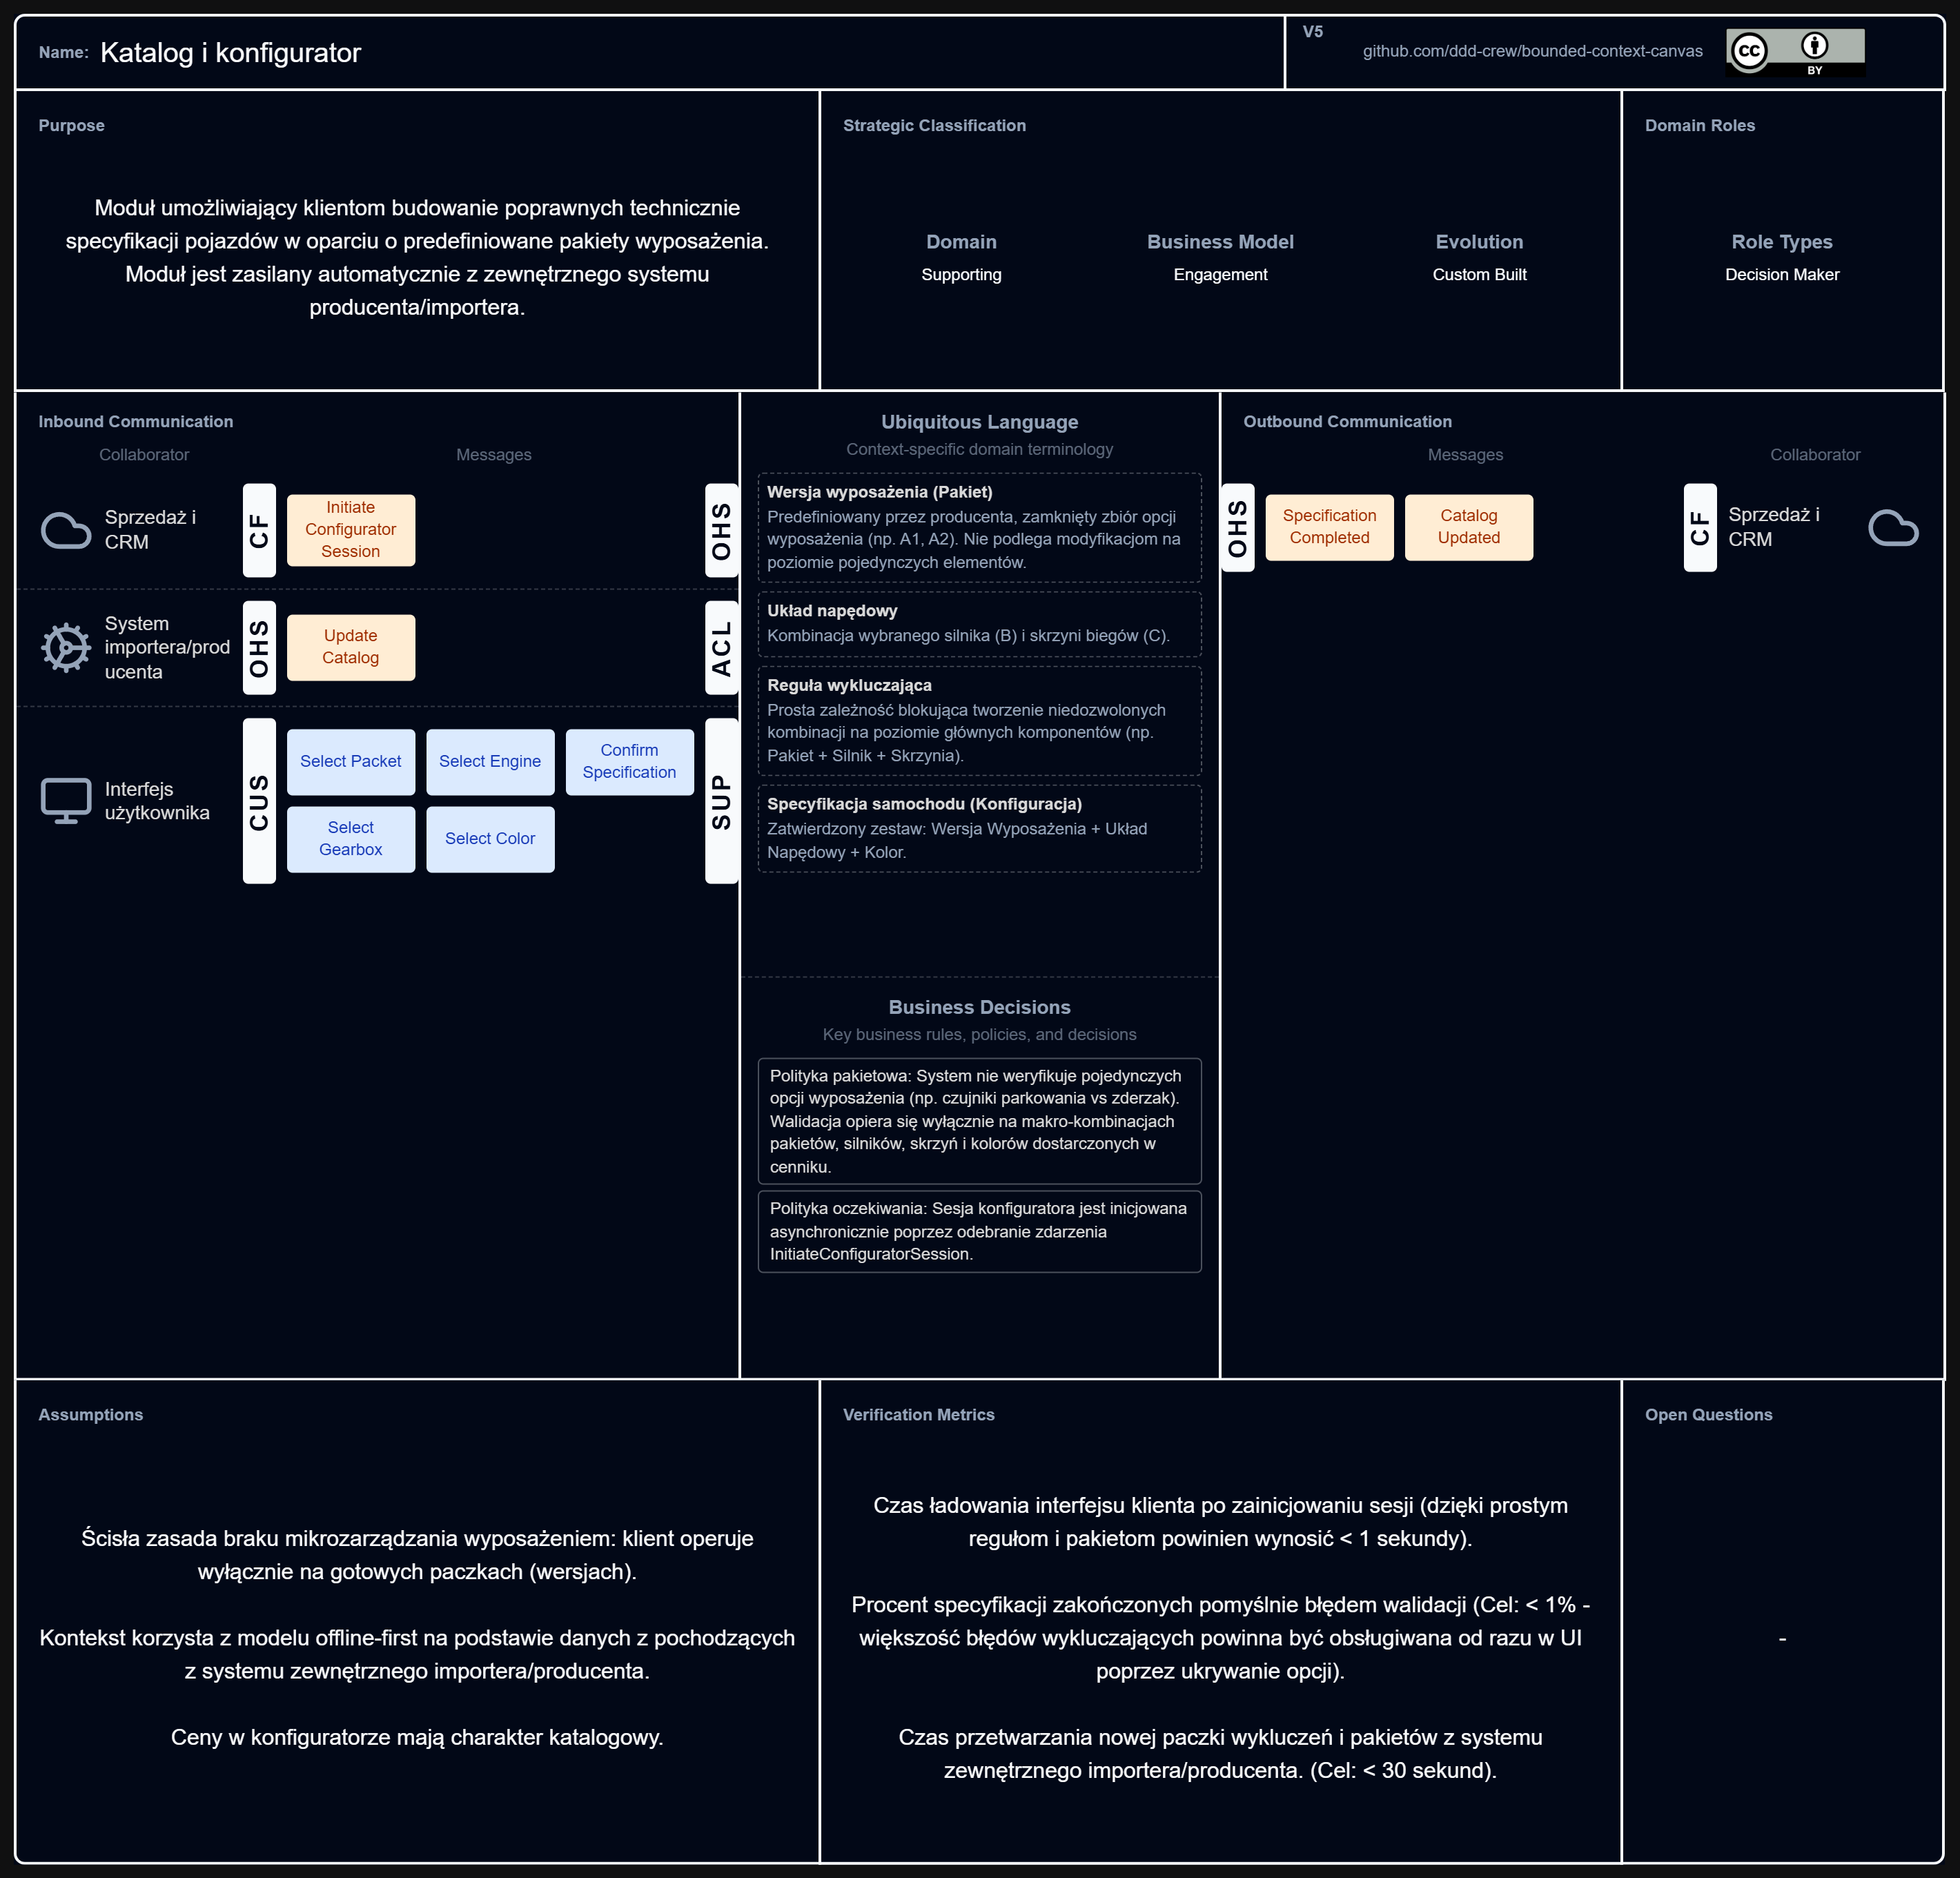
\includegraphics[width=\textwidth]{media/bounded-context-canvas/final/KIK_K2_TOTAL_FINAL.png}
    \caption{Kanwa Kontekstu  Katalogu i konfiguratora}
    \label{fig:hex_billing}
\end{figure}


\subsubsection{Przypadki użycia Kontekstu Katalogu i konfiguratora}
% =====================================================
\textbf{UC-KON-01: Opracowanie i zatwierdzenie specyfikacji pojazdu}

\begin{longtable}{|p{4cm}|p{11cm}|}
\hline
\textbf{Element} & \textbf{Opis} \\
\hline

Identyfikator & UC-KON-01 \\
\hline

Nazwa & Opracowanie i zatwierdzenie specyfikacji pojazdu \\
\hline

Opis & 
Proces wyboru parametrów pojazdu oparty na predefiniowanych pakietach wyposażenia, silnikach, skrzyniach biegów oraz kolorach nadwozia, zakończony zatwierdzeniem konfiguracji. \\
\hline

Aktor główny & Klient \\
\hline

Aktorzy pomocniczy & -  \\
\hline

Warunki wstępne & 
Kontekst Katalog i Konfigurator otrzymał zdarzenie \textit{InitiateConfiguratorSession}. \\
\hline

Warunki końcowe & 
Zatwierdzona specyfikacja zostaje zapisana w lokalnej bazie danych konfiguratora, a system emituje zdarzenie \textit{SpecificationCompleted}. \\
\hline

Scenariusz główny & 
\begin{enumerate}
    \item System otwiera sesję konfiguratora i prezentuje Klientowi interfejs z modelami samochodów, wersjami wyposażenia (np. pakiet A1, A2), silnikami (np. B1, B2), rodzajami skrzyni biegów (np. C1, C2) oraz kolorami.
    \item Klient wybiera jeden główny pakiet wyposażenia (np. A1).
    \item Klient dobiera do pakietu silnik (np. B1), rodzaj skrzyni biegów (np. C1) oraz kolor.
    \item System na bieżąco weryfikuje proste reguły wykluczające (np. silnik B2 nie może być wybrany ze skrzynią biegów C1).
    \item Klient zatwierdza specyfikację.
    \item System weryfikuje ostateczną kompletność konfiguracji.
    \item System zapisuje specyfikację i emituje zdarzenie \textit{SpecificationCompleted}.
\end{enumerate} \\
\hline

Scenariusze alternatywne & 
\begin{itemize}
    \item [A1] Niedozwolona kombinacja: W kroku 4 system wykrywa, że wybrana kombinacja jest zablokowana przez producenta (np. silnik B2 nie może być wybrany ze skrzynią C1). System blokuje możliwość zatwierdzenia i prosi Klienta o zmianę silnika, skrzyni biegów lub pakietu. Kontekst nie emituje zdarzenia końcowego.
    \item [A2] Przerwanie sesji: Klient opuszcza konfigurator przed zatwierdzeniem. System zapisuje konfigurację jako wersję roboczą.
\end{itemize} \\
\hline
\end{longtable}

\begin{figure}[H]
    \centering
    \includegraphics[width=1\textwidth]{media/diagramy_sekwencji/kontekst-katalog/UC-KON-01-Sekwencji.png}
    \caption{Diagram sekwencji dla przypadku użycia UC-KON-01: Opracowanie i zatwierdzenie specyfikacji pojazdu}
    \label{fig:seq_uc_kon_01}
\end{figure}

% =====================================================
\textbf{UC-KON-02: Automatyczna aktualizacja cennika i katalogu}

\begin{longtable}{|p{4cm}|p{11cm}|}
\hline
\textbf{Element} & \textbf{Opis} \\
\hline

Identyfikator & UC-KON-02 \\
\hline

Nazwa & Automatyczna aktualizacja cennika i katalogu \\
\hline

Opis & 
Zautomatyzowany proces pobierania, walidacji i zapisu nowego katalogu modeli oraz cennika, inicjowany przez zewnętrzny system producenta/importera (Blackbox). \\
\hline

Aktor główny & Zewnętrzny system producenta/importera \\
\hline

Aktorzy pomocniczy & - \\
\hline

Warunki wstępne & 
System zewnętrzny importera/producenta udostępnia nowy pakiet danych katalogowych (np. poprzez webhook, szynę zdarzeń lub API). \\
\hline

Warunki końcowe & 
Lokalna baza konfiguratora zostaje zaktualizowana, a kontekst emituje zdarzenie \textit{CatalogUpdated}. \\
\hline

Scenariusz główny & 
\begin{enumerate}
    \item Kontekst odbiera sygnał/dane o nowym cenniku z systemu Blackbox (np. poprzez zdarzenie integracyjne lub żądanie API).
    \item System parsuje otrzymany pakiet danych, wykorzystując warstwę translacji (ACL), aby dostosować format zewnętrzny do modelu lokalnego.
    \item System przeprowadza walidację strukturalną oraz logiczną (weryfikacja spójności reguł wyposażenia i poprawności cen).
    \item System zapisuje nowy katalog w lokalnej bazie danych, zastępując bieżące dane (poprzednie zostają oznaczone jako archiwalne).
    \item Kontekst emituje na szynę danych zdarzenie \textit{CatalogUpdated}.
\end{enumerate} \\
\hline

Scenariusze alternatywne & 
\begin{itemize}
    \item [A1] Błąd walidacji lub translacji danych: W kroku 2 lub 3 system wykrywa błędy krytyczne (np. brak cen, niezgodny format). System przerywa aktualizację, odrzuca pakiet i emituje techniczne zdarzenie o błędzie integracji (np. \textit{CatalogUpdateFailed}), logując szczegóły dla wsparcia IT.
\end{itemize} \\
\hline
\end{longtable}

\begin{figure}[H]
    \centering
    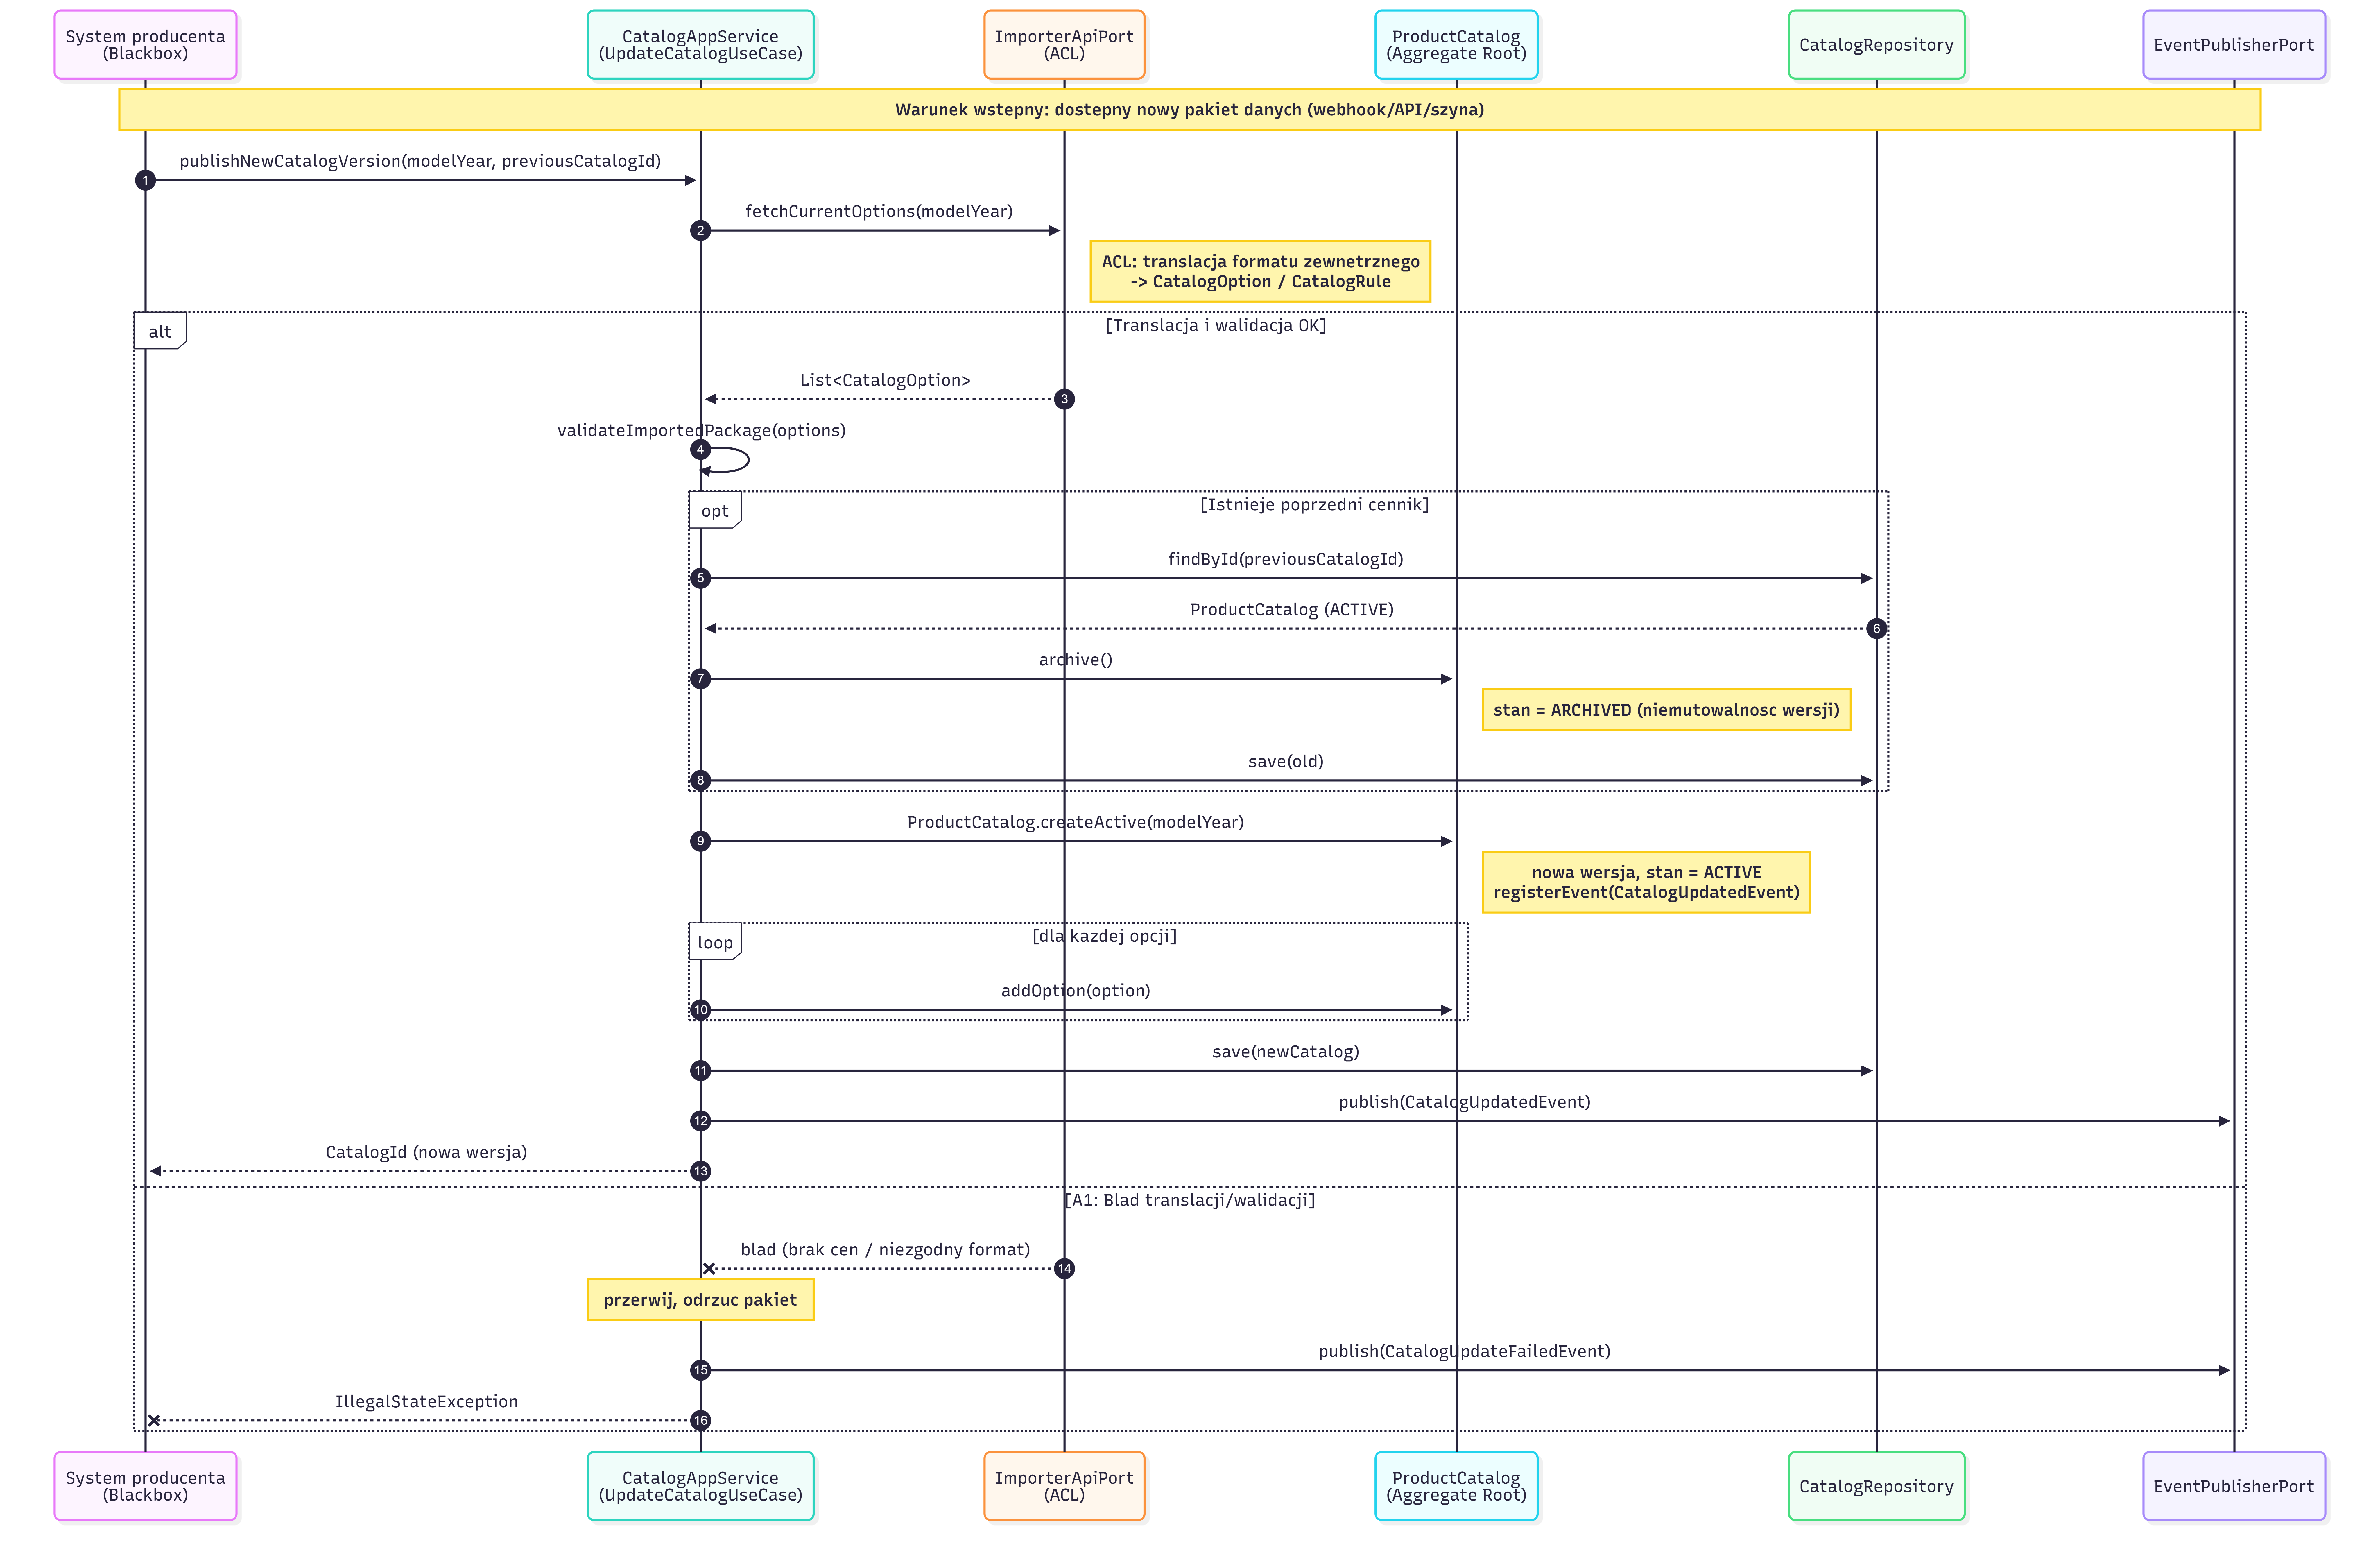
\includegraphics[width=1\textwidth]{media/diagramy_sekwencji/kontekst-katalog/UC-KON-02-Sekwencji.png}
    \caption{Diagram sekwencji dla przypadku użycia UC-KON-02: Automatyczna aktualizacja cennika i katalogu}
    \label{fig:seq_uc_kon_02}
\end{figure}

\subsubsection{Architektura Kontekstu Katalogu i Konfiguratora}

Kontekst Katalogu i Konfiguratora został zaprojektowany w oparciu o architekturę heksagonalną. Diagram Architektury przedstawiono na rysunku \ref{fig:hex_catalog}.

% MIEJSCE NA DIAGRAM ARCHITEKTURY (Katalog Flowchart)
\begin{figure}[H]
    \centering
    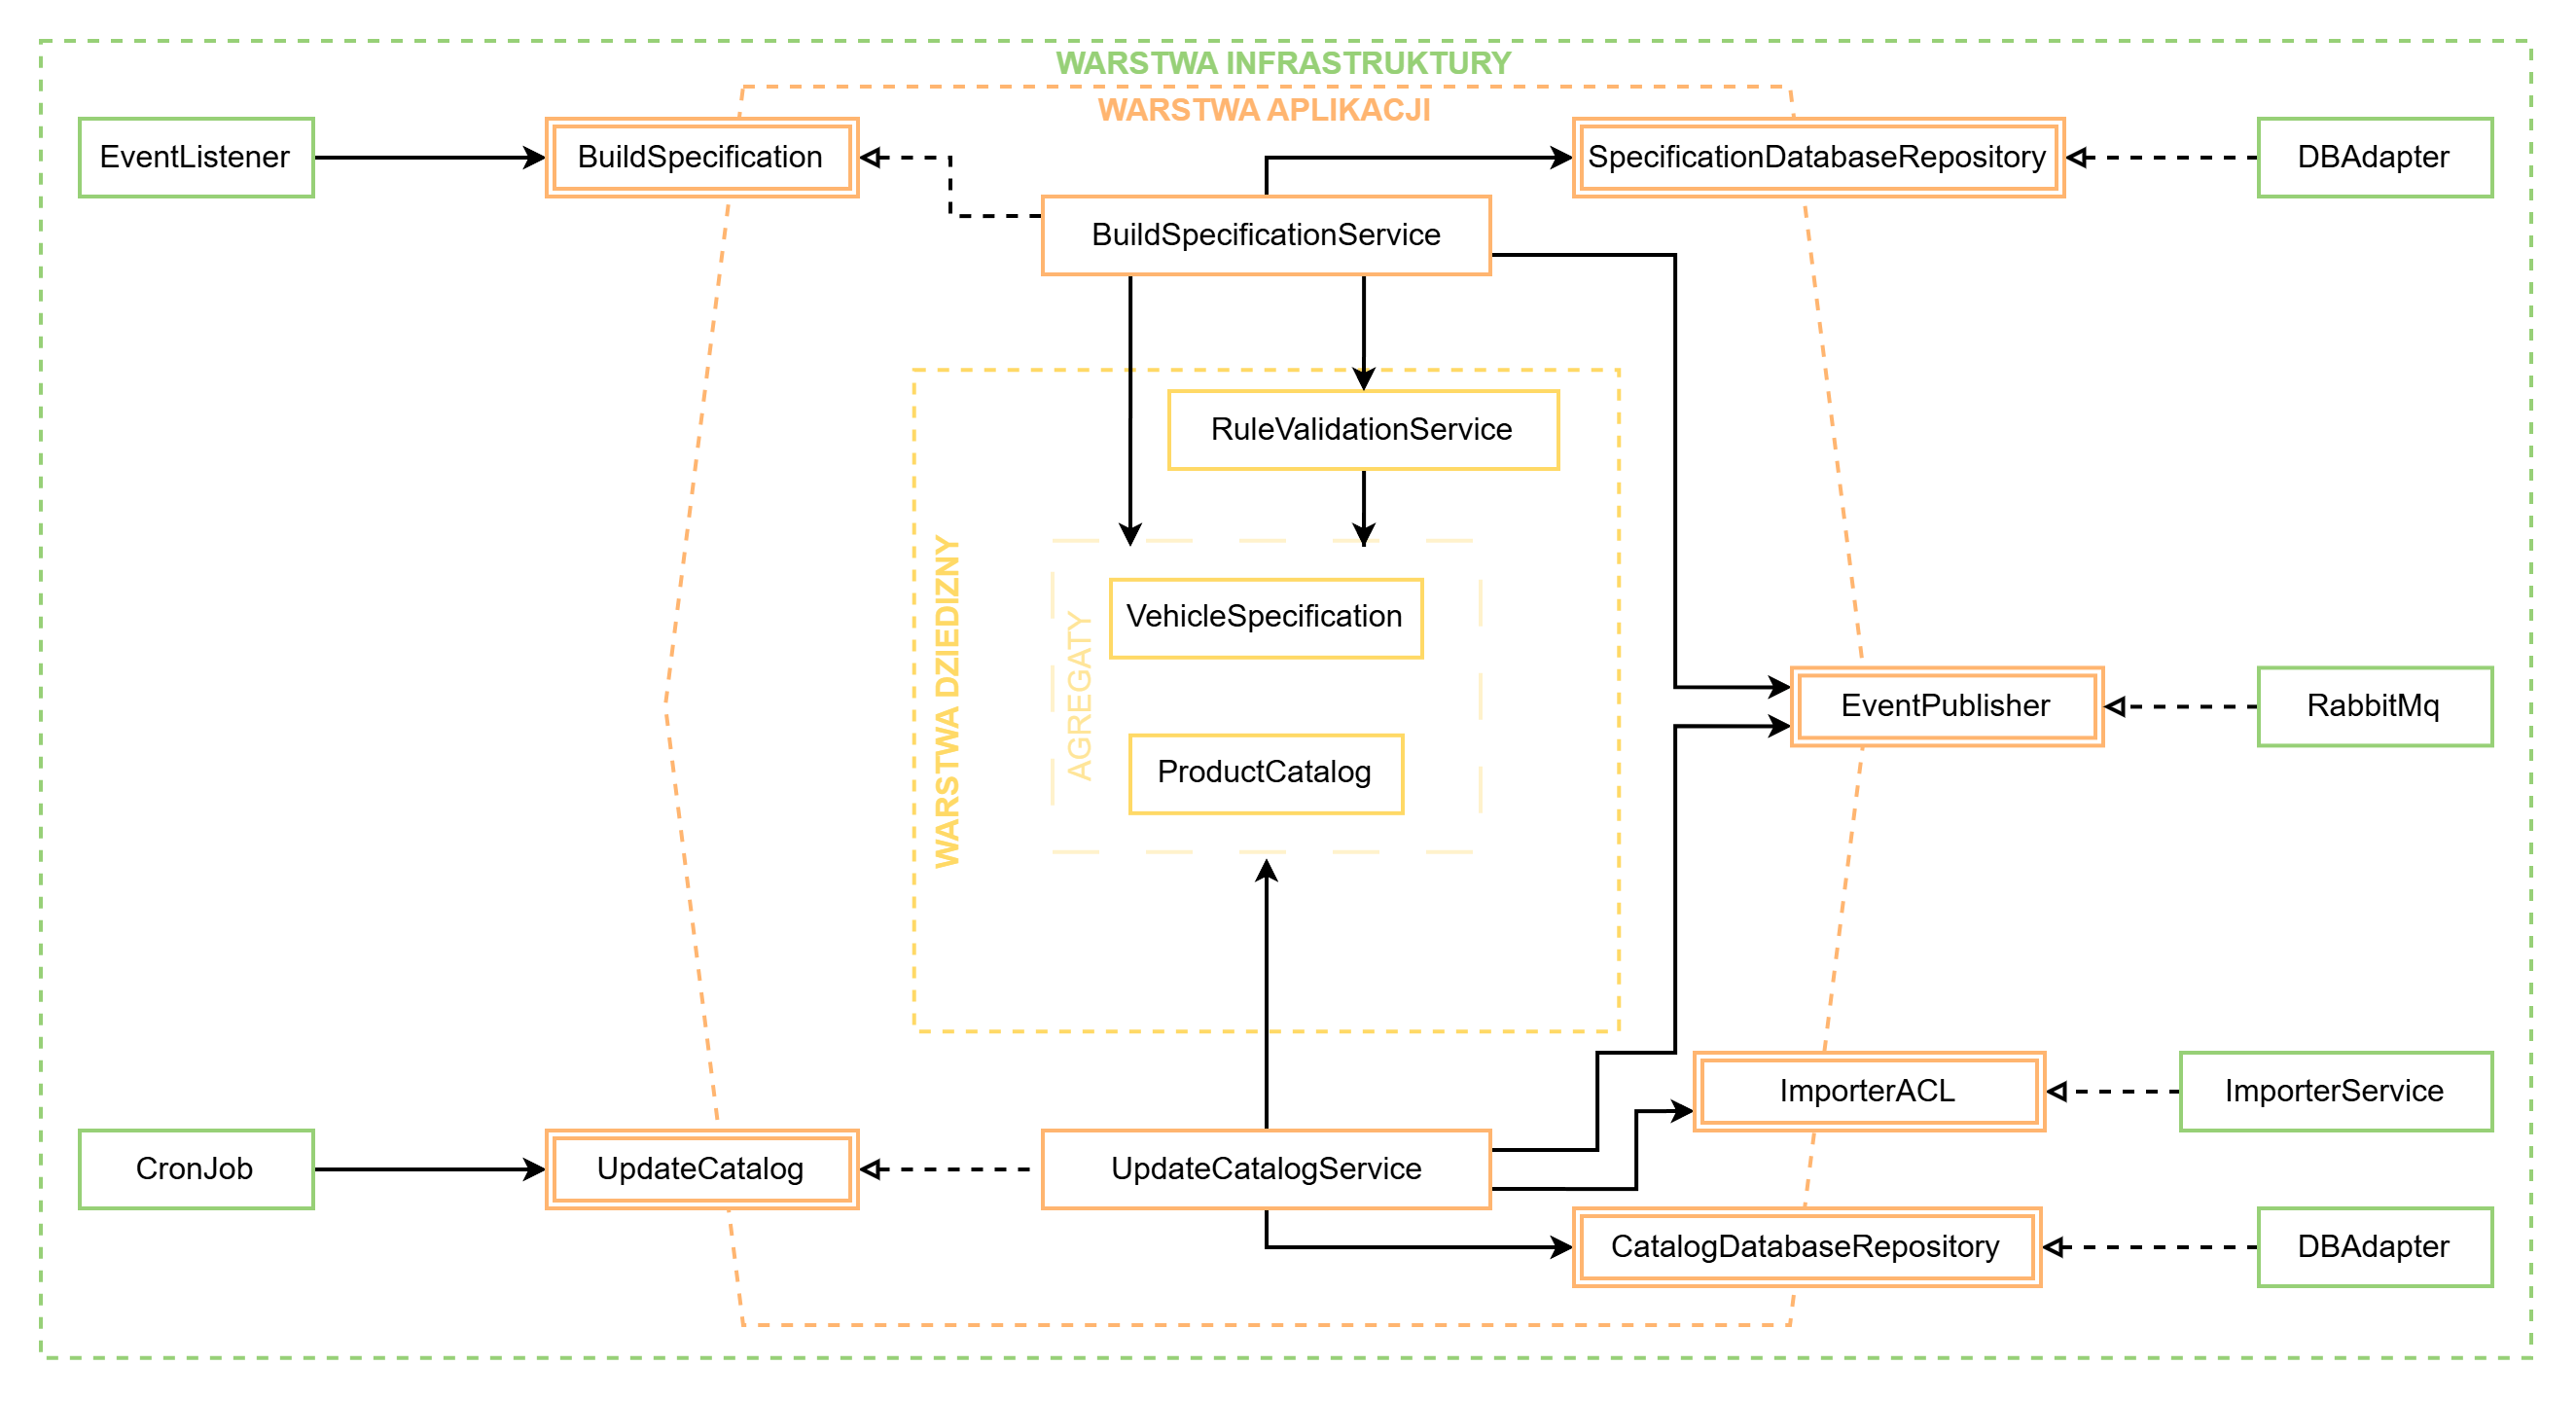
\includegraphics[width=\textwidth]{media/architektura_heksagonalna/CatalogArchitecture.png}
    \caption{Struktura portów i adapterów dla Kontekstu Katalogu i Konfiguratora}
    \label{fig:hex_catalog}
\end{figure}

Poniżej przedstawiono szczegółowy opis interakcji pomiędzy warstwami, z podziałem na strony wejściową i wyjściową.

\paragraph{Strona Wejściowa: Porty i Adaptery} 
Ta strona heksagonu definiuje wejścia do systemu, oddzielając ruch interaktywny od użytkowników od technicznych sygnałów inicjujących aktualizacje.

\begin{itemize}
    \item \textbf{Zarządzanie Specyfikacją Pojazdu (Interaktywne)}
    \begin{itemize}
        \item \textbf{Port:} \texttt{BuildSpecification}. Pojedynczy interfejs obsługujący główny przepływ biznesowy klienta — inicjację (\texttt{startSpecification}), dobór opcji (\texttt{addOption}) i zatwierdzenie (\texttt{finalizeSpecification}) konfiguracji (UC-KON-01). Realizowany centralnie przez \texttt{BuildSpecificationService}.
        \item \textbf{Adapter:} \texttt{ConfiguratorEventListener}. Adapter wejściowy nasłuchujący zdarzeń konfiguratora i tłumaczący je na komendy mutujące stan specyfikacji.
    \end{itemize}

    \item \textbf{Synchronizacja Cennika (Automatyczna)}
    \begin{itemize}
        \item \textbf{Port:} \texttt{UpdateCatalog}. Interfejs inicjujący proces bezpiecznego pobrania i wgrania nowej bazy modelowej (UC-KON-02). Realizowany wyłącznie przez \texttt{UpdateCatalogService}.
        \item \textbf{Adapter:} \texttt{CatalogUpdateScheduler}. Techniczny adapter asynchroniczny wykorzystujący harmonogram zadań, uruchamiający cykliczny proces synchronizacji bazy bez udziału operatora.
    \end{itemize}
\end{itemize}

\paragraph{Strona Wyjściowa: Porty i Adaptery} 
Ta strona heksagonu zarządza utrwalaniem zwalidowanych danych we własnej bazie oraz wymianą danych z globalnym systemem producenta.

\begin{itemize}
    \item \textbf{Integracja z Producentem (Warstwa Ochronna)}
    \begin{itemize}
        \item \textbf{Port:} \texttt{CatalogImporterPort}. Interfejs służący do pobierania zewnętrznych danych o regułach, opcjach i cenach.
        \item \textbf{Adapter:} \texttt{ImporterAclAdapter} (wraz z \texttt{ImporterServiceClient}, \texttt{ImporterCatalogTranslator}, \texttt{ExternalCatalogPackage}). Implementuje wzorzec Anti-Corruption Layer — tłumaczy zagnieżdżone, potencjalnie niestabilne struktury API dostawcy na czysty, wewnętrzny model obiektów wartości, izolując rdzeń katalogu od zmian formatu u importera.
    \end{itemize}

    \item \textbf{Utrwalanie Stanu (Persystencja)}
    \begin{itemize}
        \item \textbf{Porty:} \texttt{VehicleSpecificationRepository} oraz \texttt{ProductCatalogRepository}. Umożliwiają trwały zapis odpowiednio konfigurowanych specyfikacji aut oraz wersjonowanych wydań katalogów.
        \item \textbf{Adaptery:} \texttt{SpecificationDatabaseRepository} oraz \texttt{CatalogDatabaseRepository} (z mapperami \texttt{*PersistenceMapper} i rekordami \texttt{*Record} oraz \texttt{DbAdapter}/\texttt{InMemoryDbAdapter}). Mapują grafy obiektów domenowych na rekordy magazynu, gwarantując zapis z zachowaniem spójności; w bieżącej implementacji warstwą bazową jest \texttt{InMemoryDbAdapter}.
    \end{itemize}

    \item \textbf{Publikacja Zdarzeń (Event Driven)}
    \begin{itemize}
        \item \textbf{Port:} \texttt{EventPublisher}. Umożliwia publikację zdarzeń wynikowych na magistralę.
        \item \textbf{Adapter:} \texttt{RabbitMqEventPublisher} (wraz z \texttt{MessageBroker}). Serializuje zdarzenia dziedzinowe (np. \texttt{SpecificationCompleted}, \texttt{CatalogUpdated}) i wysyła je na magistralę.
    \end{itemize}
\end{itemize}

\paragraph{Usługi Aplikacji}
Ze względu na konieczność separacji procesu tworzenia cennika od procesu jego konsumpcji, wyodrębniono tu dwa niezależne orkiestratory:
\begin{itemize}
    \item \textbf{BuildSpecificationService} – zarządza cyklem życia agregatu \texttt{VehicleSpecification}. Przechwytuje żądania użytkownika, deleguje rygorystyczną weryfikację reguł wykluczających do serwisu domenowego, a po ostatecznym zatwierdzeniu utrwala specyfikację i emituje fakt o ukończeniu konfiguracji (\texttt{SpecificationCompleted}).
    \item \textbf{UpdateCatalogService} – orkiestruje proces zapisu cennika. Zamiast nadpisywać istniejące dane, tworzy nową instancję agregatu \texttt{ProductCatalog} z podbitą wersją, oznaczając stary katalog jako archiwalny, co chroni integralność historycznych zamówień, i emituje \texttt{CatalogUpdated}.
\end{itemize}

\paragraph{Usługi Domenowe}
Ze względu na złożoność wykluczeń inżynieryjnych (np. niekompatybilność danego silnika z konkretną skrzynią biegów), wdrożono dedykowany serwis bezstanowy:
\begin{itemize}
    \item \textbf{RuleValidationService} – izoluje skomplikowaną logikę weryfikacyjną. Zgodnie z zasadami projektowania domenowego agregat specyfikacji nie posiada wiedzy o zewnętrznym cenniku — to serwis aplikacyjny deleguje walidację do tego serwisu domenowego, który (sam pobierając katalog z repozytorium) ocenia legalność wybranych kombinacji kodów opcji przed przejściem do stanu końcowego.
\end{itemize}

\subsubsection{Agregaty Kontekstu Katalogu i Konfiguratora}

Aby zapewnić odporność systemu na zmianę cen w trakcie długotrwałego procesu ofertowania, zastosowano twardy rozdział pomiędzy słownikiem reguł a koszykiem konfiguracyjnym użytkownika, tworząc dwa oddzielne agregaty.

% MIEJSCE NA DIAGRAM KLAS: ProductCatalog
\begin{figure}[H]
    \centering
    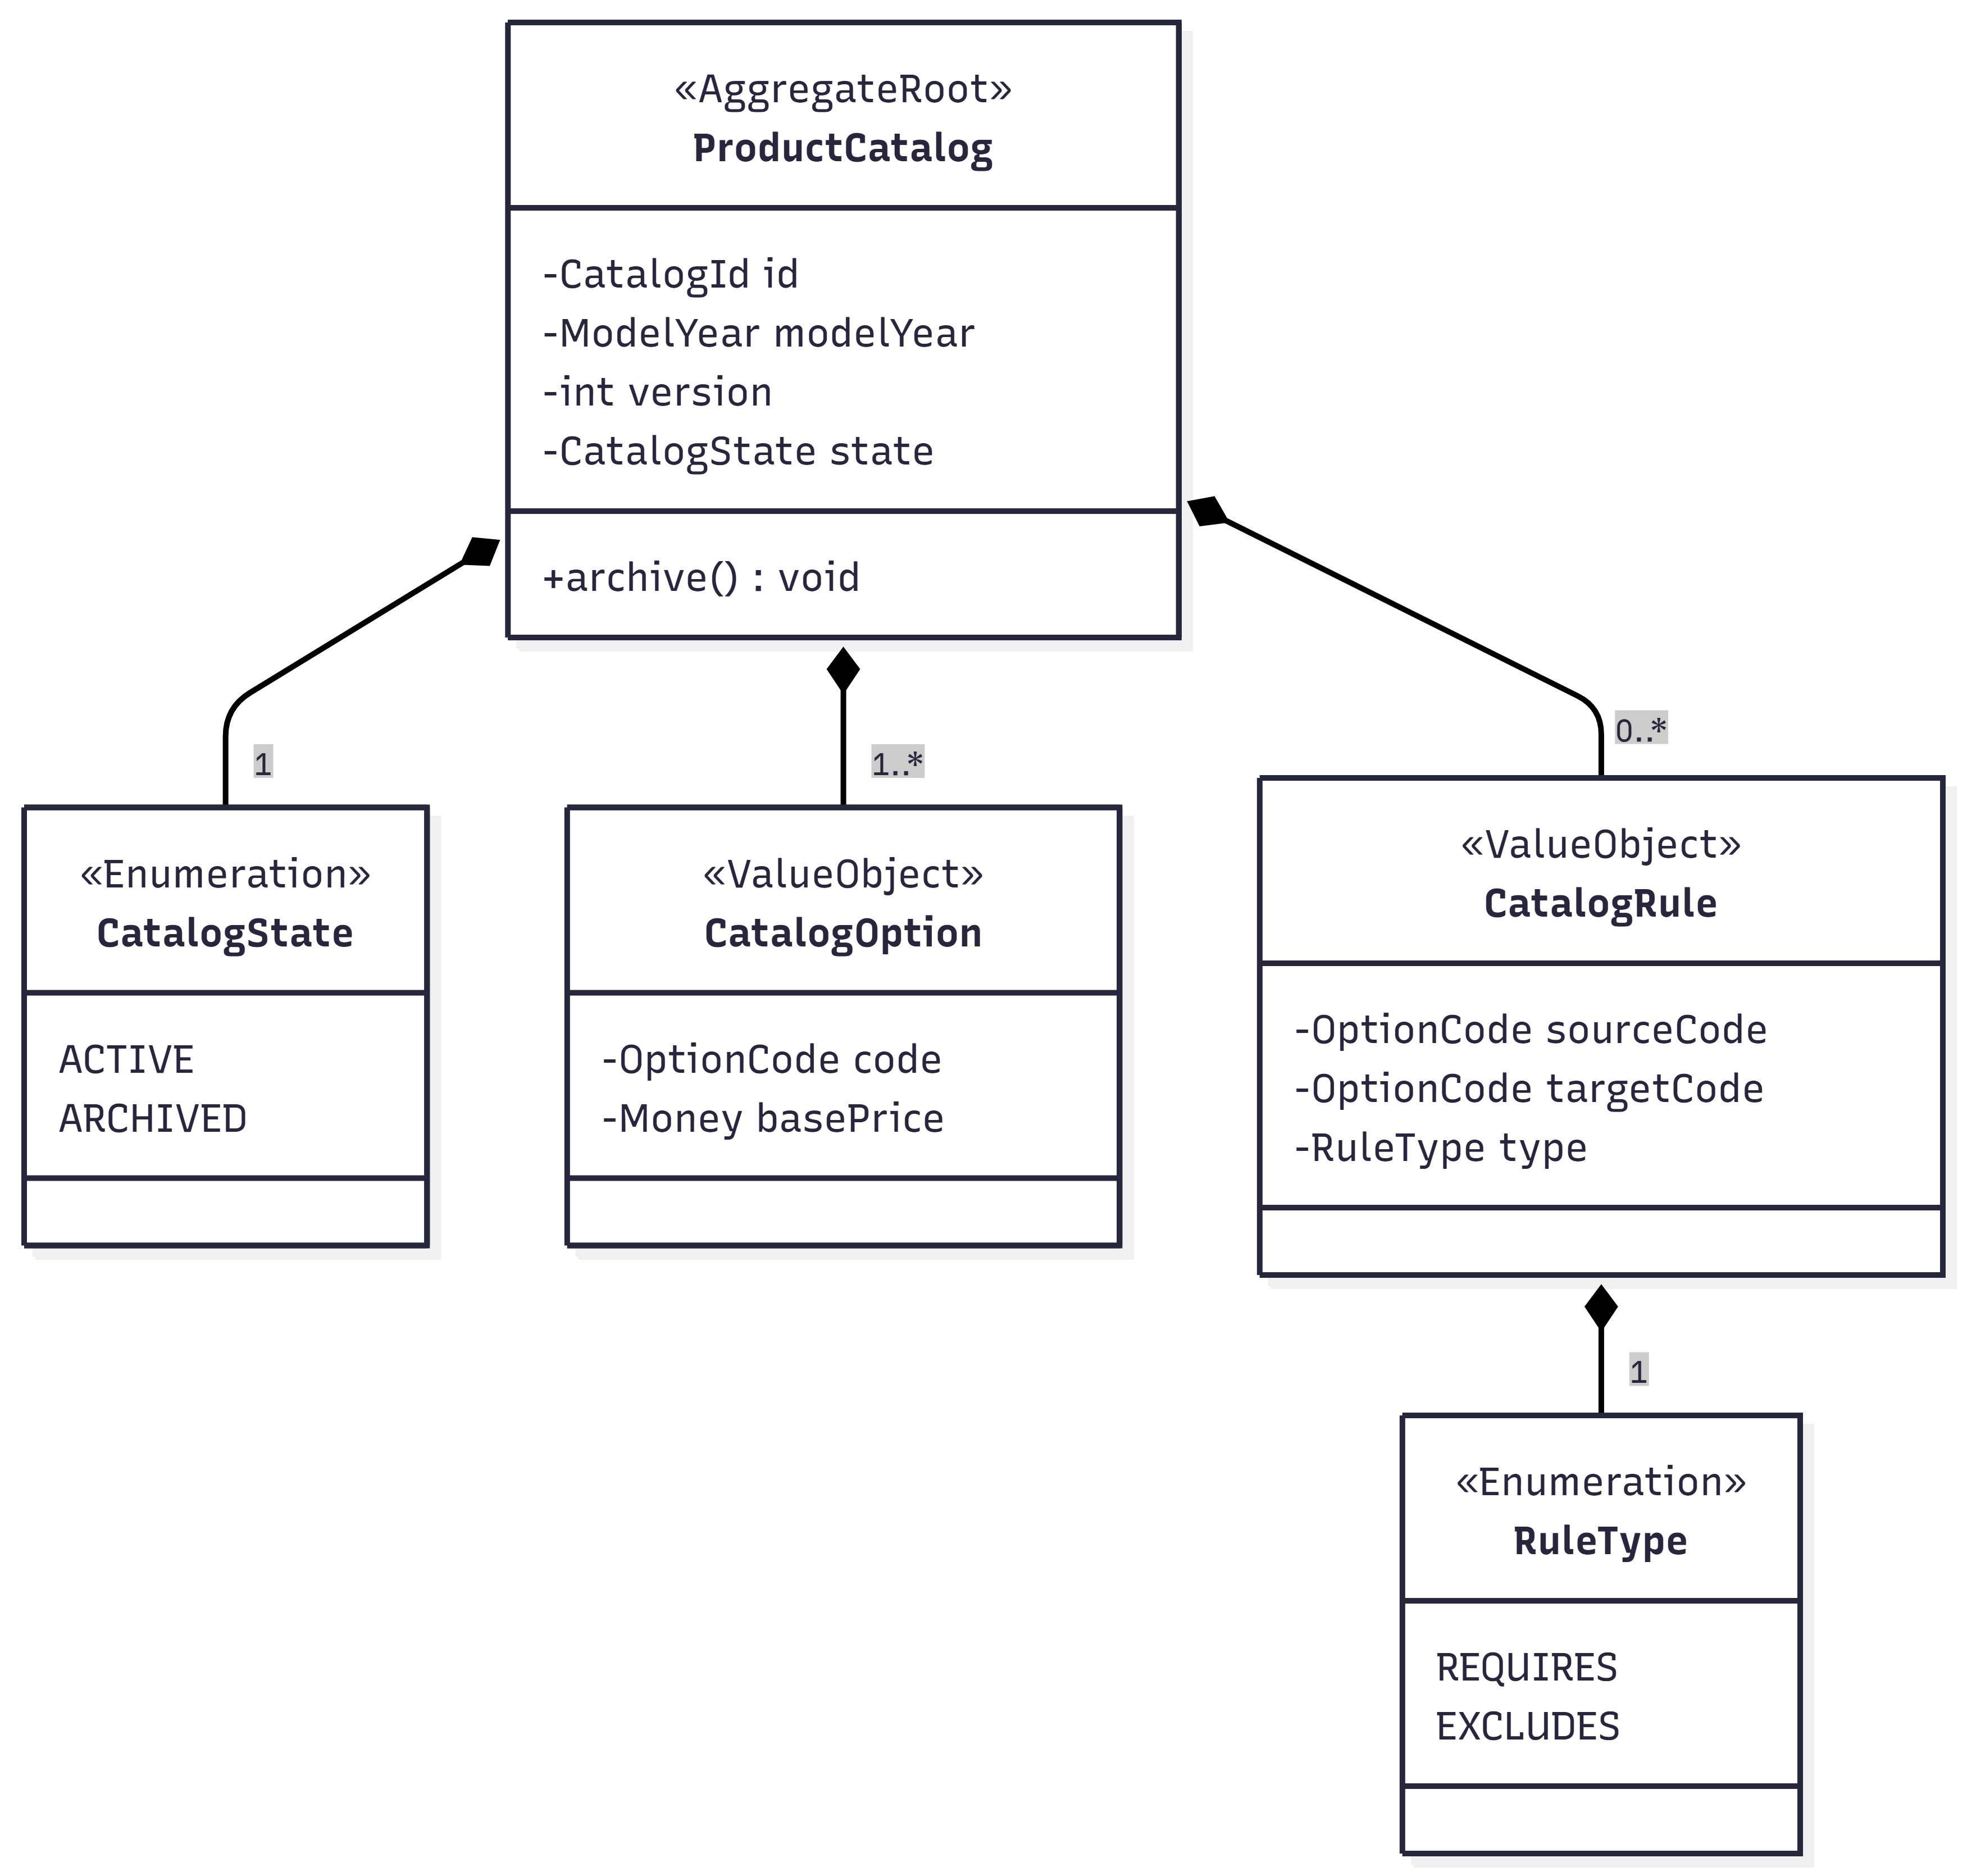
\includegraphics[width=0.49\textwidth]{media/agregaty/kontekst-katalogu/product-catalog.png}
    \hfill
    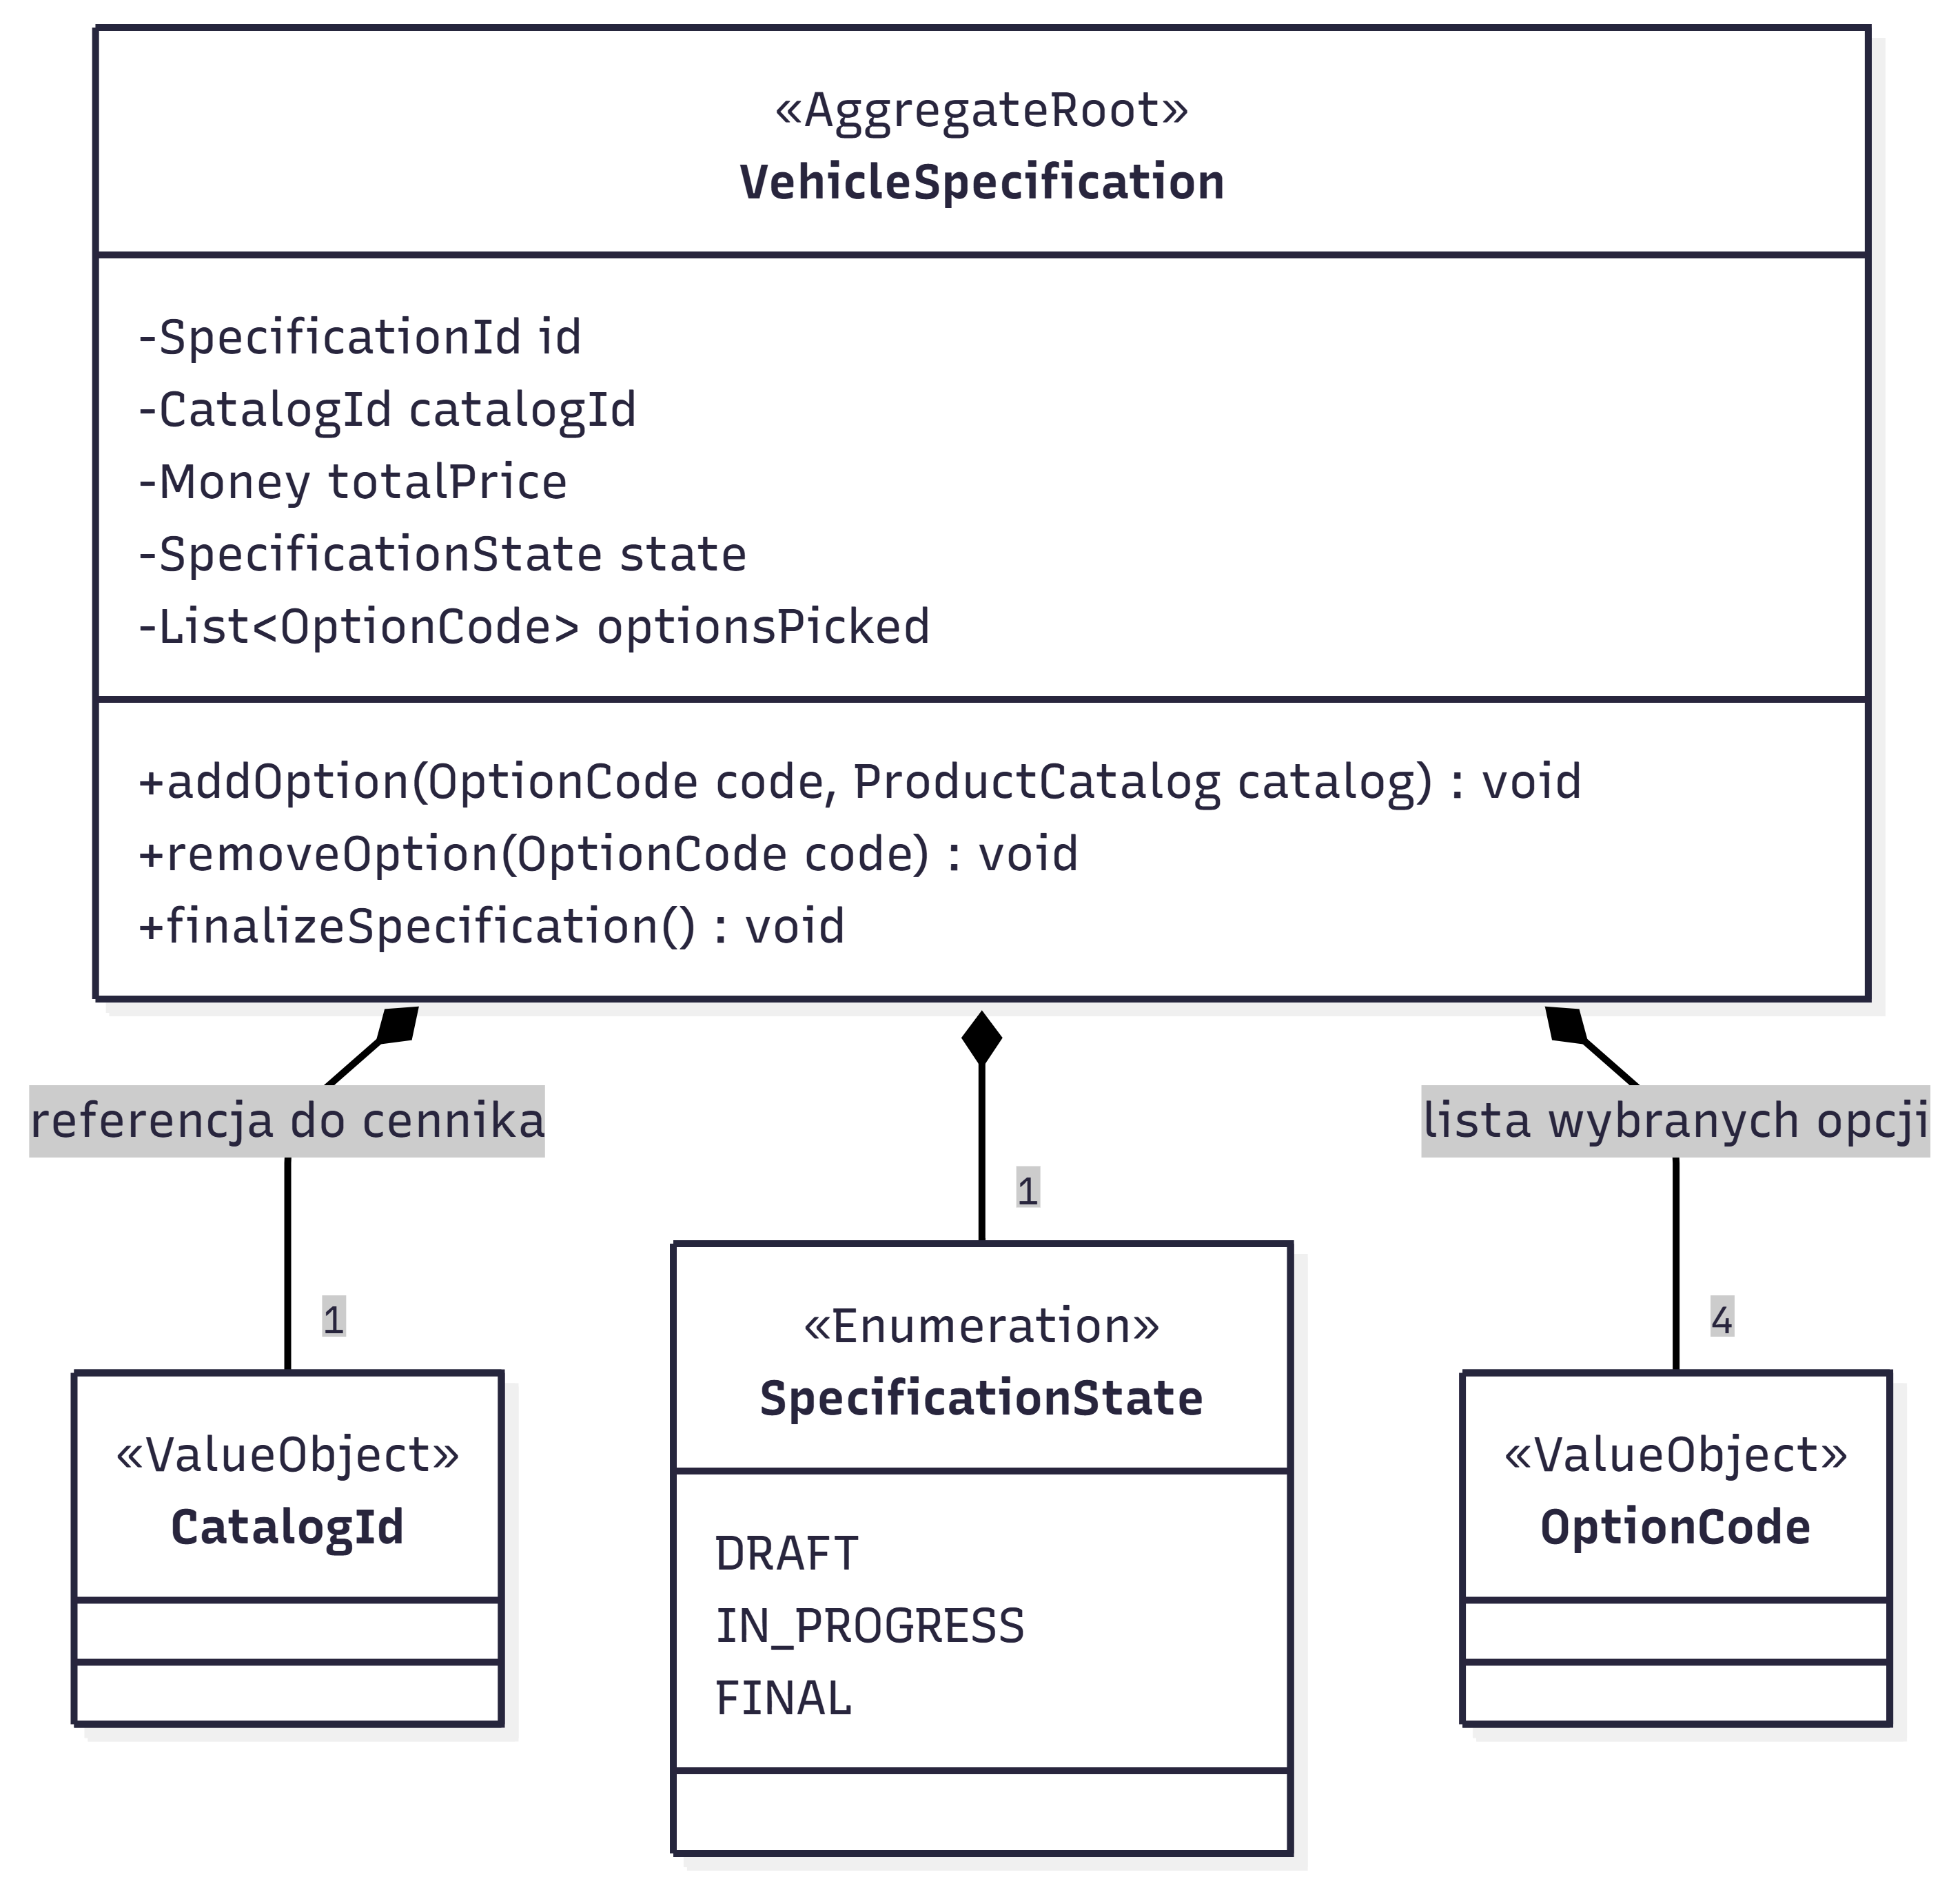
\includegraphics[width=0.49\textwidth]{media/agregaty/kontekst-katalogu/vehicle-spec.png}
    \caption{Model strukturalny agregatu Matrycy Produkcyjnej}
    \label{fig:agg_product_catalog}
\end{figure}

\paragraph{Agregat: Matryca Produkcyjna / Cennik (ProductCatalog)}
Agregat ten stanowi kompletny zbiór opcji (\texttt{CatalogOption}) i reguł zależności (\texttt{CatalogRule}) przypisany do danego rocznika modelowego.
\begin{itemize}
    \item \textbf{Ochrona Niezmienników (Niemutowalność wersji):} Cennik będący w stanie \texttt{ACTIVE} jest obiektem ściśle niemutowalnym. Jakakolwiek aktualizacja cen lub reguł pobrana z API producenta nie może nadpisać aktywnego obiektu -- wzorzec fabryki wymusza stworzenie nowej wersji (\texttt{version}) agregatu i dearchiwizację starej. Gwarantuje to, że historyczne specyfikacje klientów zachowują bezwzględną spójność z cennikiem, z którego zostały wygenerowane.
    \item \textbf{Polityka pakietowa:} Zgodnie z założeniami biznesowymi, słownik \texttt{OptionCode} nie operuje na pojedynczych elementach (tzw. mikrozarządzanie wyposażeniem), lecz na bazie predefiniowanych zbiorów (np. Wersja Wyposażenia, Silnik, Skrzynia Biegów, Kolor). Znacznie optymalizuje to wydajność mechanizmów walidacyjnych w systemie.
\end{itemize}

\paragraph{Agregat: Specyfikacja Pojazdu (VehicleSpecification)}
Reprezentuje unikalną konfigurację budowaną przez klienta lub handlowca, identyfikowaną przez globalny unikalny numer \texttt{SpecificationId}.
\begin{itemize}
    \item \textbf{Maszyna Stanów i Kompletność (\texttt{IN\_PROGRESS}):} Specyfikacja podlega ścisłemu cyklowi stanowemu. Początkowo tworzona jest jako pusty \texttt{DRAFT}. Gdy użytkownik rozpoczyna wybór opcji, agregat przechodzi w stan \texttt{IN\_PROGRESS}. Stan ten oznacza, że konfiguracja jest w toku budowy i nie posiada jeszcze kompletu wymaganych do produkcji makro-opcji (np. brakuje wyboru docelowego silnika, skrzyni biegów czy koloru).
    \item \textbf{Ochrona Niezmienników (Walidacja Technologiczna):} Próba dodania nowej opcji wyposażenia (metoda \texttt{addOption}) na bieżąco weryfikuje lokalną listę wybranych kodów względem reguł (\texttt{EXCLUDES}, \texttt{REQUIRES}) dostarczonych przez serwis domenowy na podstawie cennika. Złamanie reguły natychmiastowo blokuje operację (wzo

\newpage
\subsection{Kontekst Inwentarza i Logistyki}
Kontekst Inwentarza i Logistyki to poddziedzina wspierająca, której nadrzędnym celem jest odwzorowanie w systemie informatycznym fizycznego stanu placu dealerskiego oraz statusu aut znajdujących się w produkcji. To w tym module krzyżują się procesy logistyczne realizowane przez pracowników placu z decyzjami biznesowymi z Kontekstu Sprzedaży.

\subsubsection{Kanwa Kontekstu Inwentarza i logistyki pojazdów}
\begin{figure}[H]
    \centering
    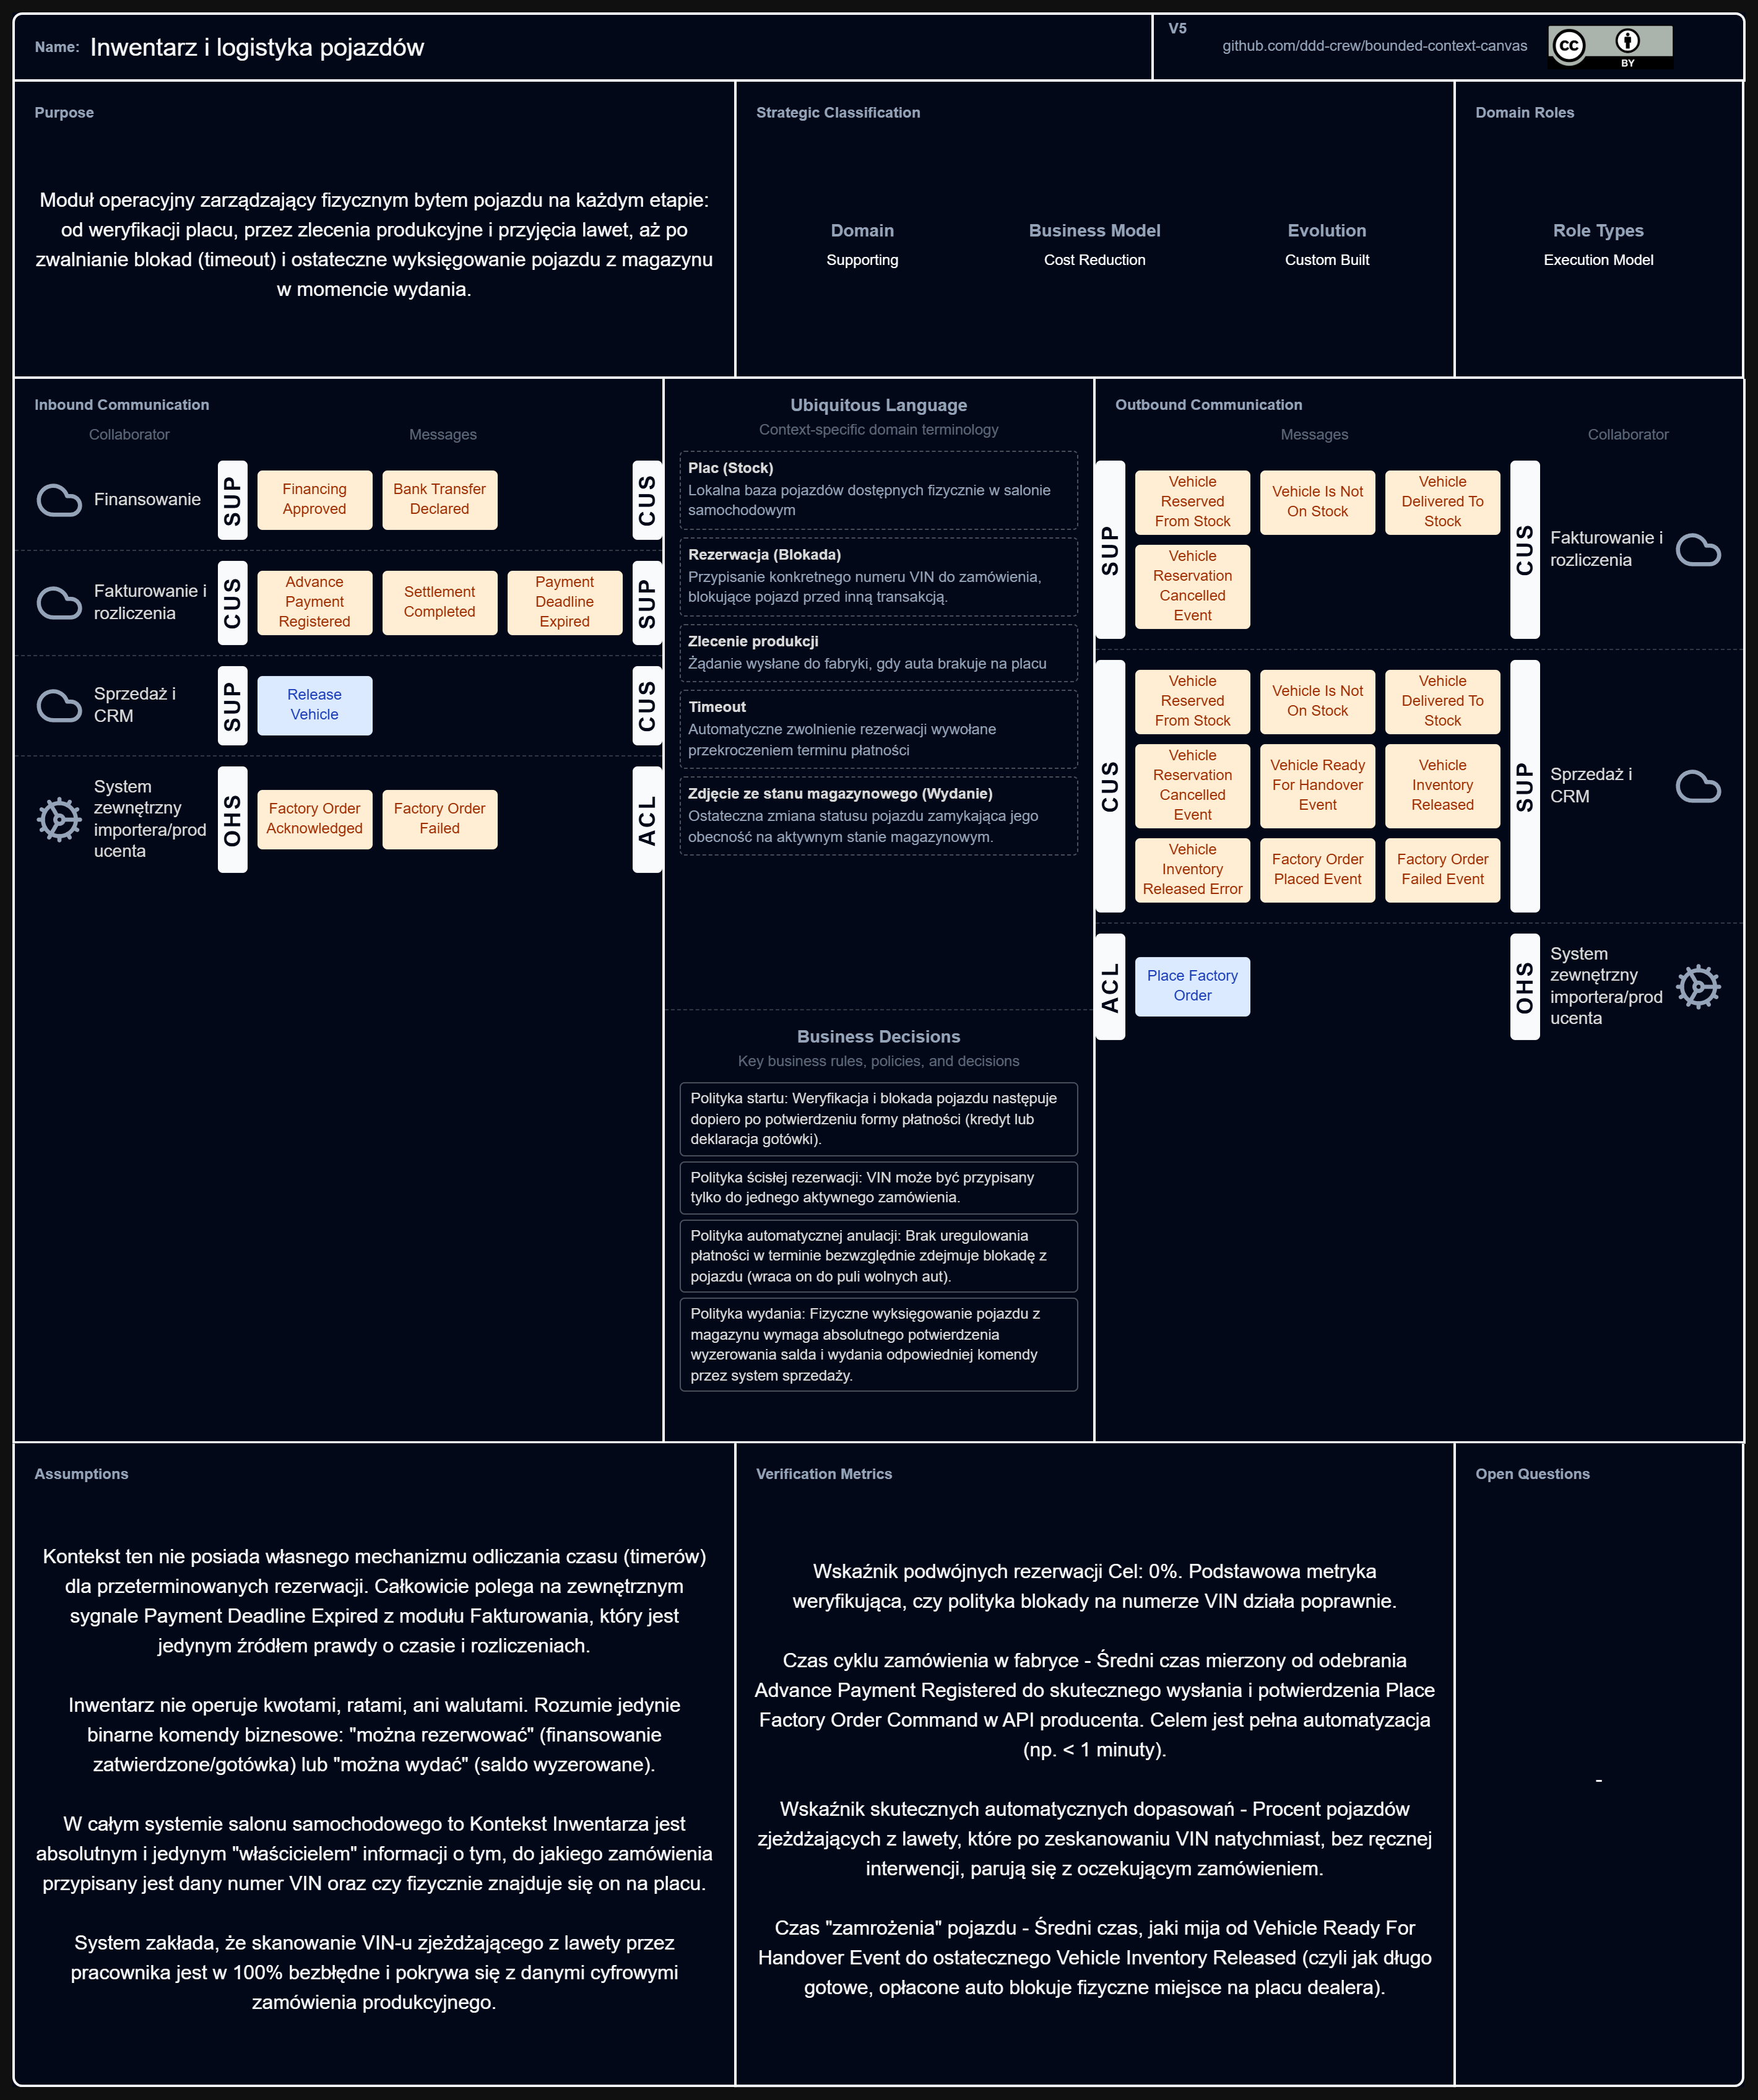
\includegraphics[width=\textwidth]{media/bounded-context-canvas/final/IiLP_K3_TOTAL_FINAL.png}
    \caption{Kanwa Kontekstu  Inwentarza i logistyki pojazdów}
    \label{fig:hex_billing}
\end{figure}
\subsubsection{Przypadki użycia Inwentarza i logistyki pojazdów}

\textbf{UC-INW-01: Weryfikacja dostępności i rezerwacja pojazdu z placu}

\begin{longtable}{|p{4cm}|p{11cm}|}
\hline
\textbf{Element} & \textbf{Opis} \\
\hline

Identyfikator & UC-INW-01 \\
\hline

Nazwa & Weryfikacja dostępności i rezerwacja pojazdu z placu \\
\hline

Opis & 
Sprawdzenie fizycznej dostępności pojazdu o wybranej specyfikacji na placu dealerskim i założenie twardej blokady (rezerwacji) na konkretny numer VIN. \\
\hline

Aktor główny & System (Kontekst Inwentarza i Logistyki) \\
\hline

Aktorzy pomocniczy & - \\
\hline

Warunki wstępne & 
Kontekst otrzymał zdarzenie potwierdzające gotowość do realizacji zamówienia \textit{FinancingApproved} LUB \textit{BankTransferDeclared}. \\
\hline

Warunki końcowe & 
Pojazd zostaje zarezerwowany, system emituje zdarzenie \textit{VehicleReservedFromStock} (dla samochodu na placu) LUB \textit{VehicleNotOnStock} (jeśli nie ma samochodu na stanie magazynowym). \\
\hline

Scenariusz główny & 
\begin{enumerate}
    \item System reaguje na zdarzenie inicjujące proces realizacji.
    \item System przeszukuje lokalną bazę pojazdów dostępnych na placu (status "Wolny") pod kątem specyfikacji z zamówienia.
    \item System znajduje pasujący pojazd i przypisuje jego numer VIN do zamówienia.
    \item System zmienia status pojazdu na "Zarezerwowany".
    \item Kontekst emituje zdarzenie \textit{VehicleReservedFromStockEvent}.
\end{enumerate} \\
\hline

Scenariusze alternatywne & 
\begin{itemize}
    \item [A1] Samochodu nie ma na placu: W kroku 2 system nie znajduje wolnego pojazdu o wymaganej specyfikacji. System wstrzymuje rezerwację i emituje zdarzenie \textit{VehicleNotOnStock}.
\end{itemize} \\
\hline
\end{longtable}

\begin{figure}[H]
    \centering
    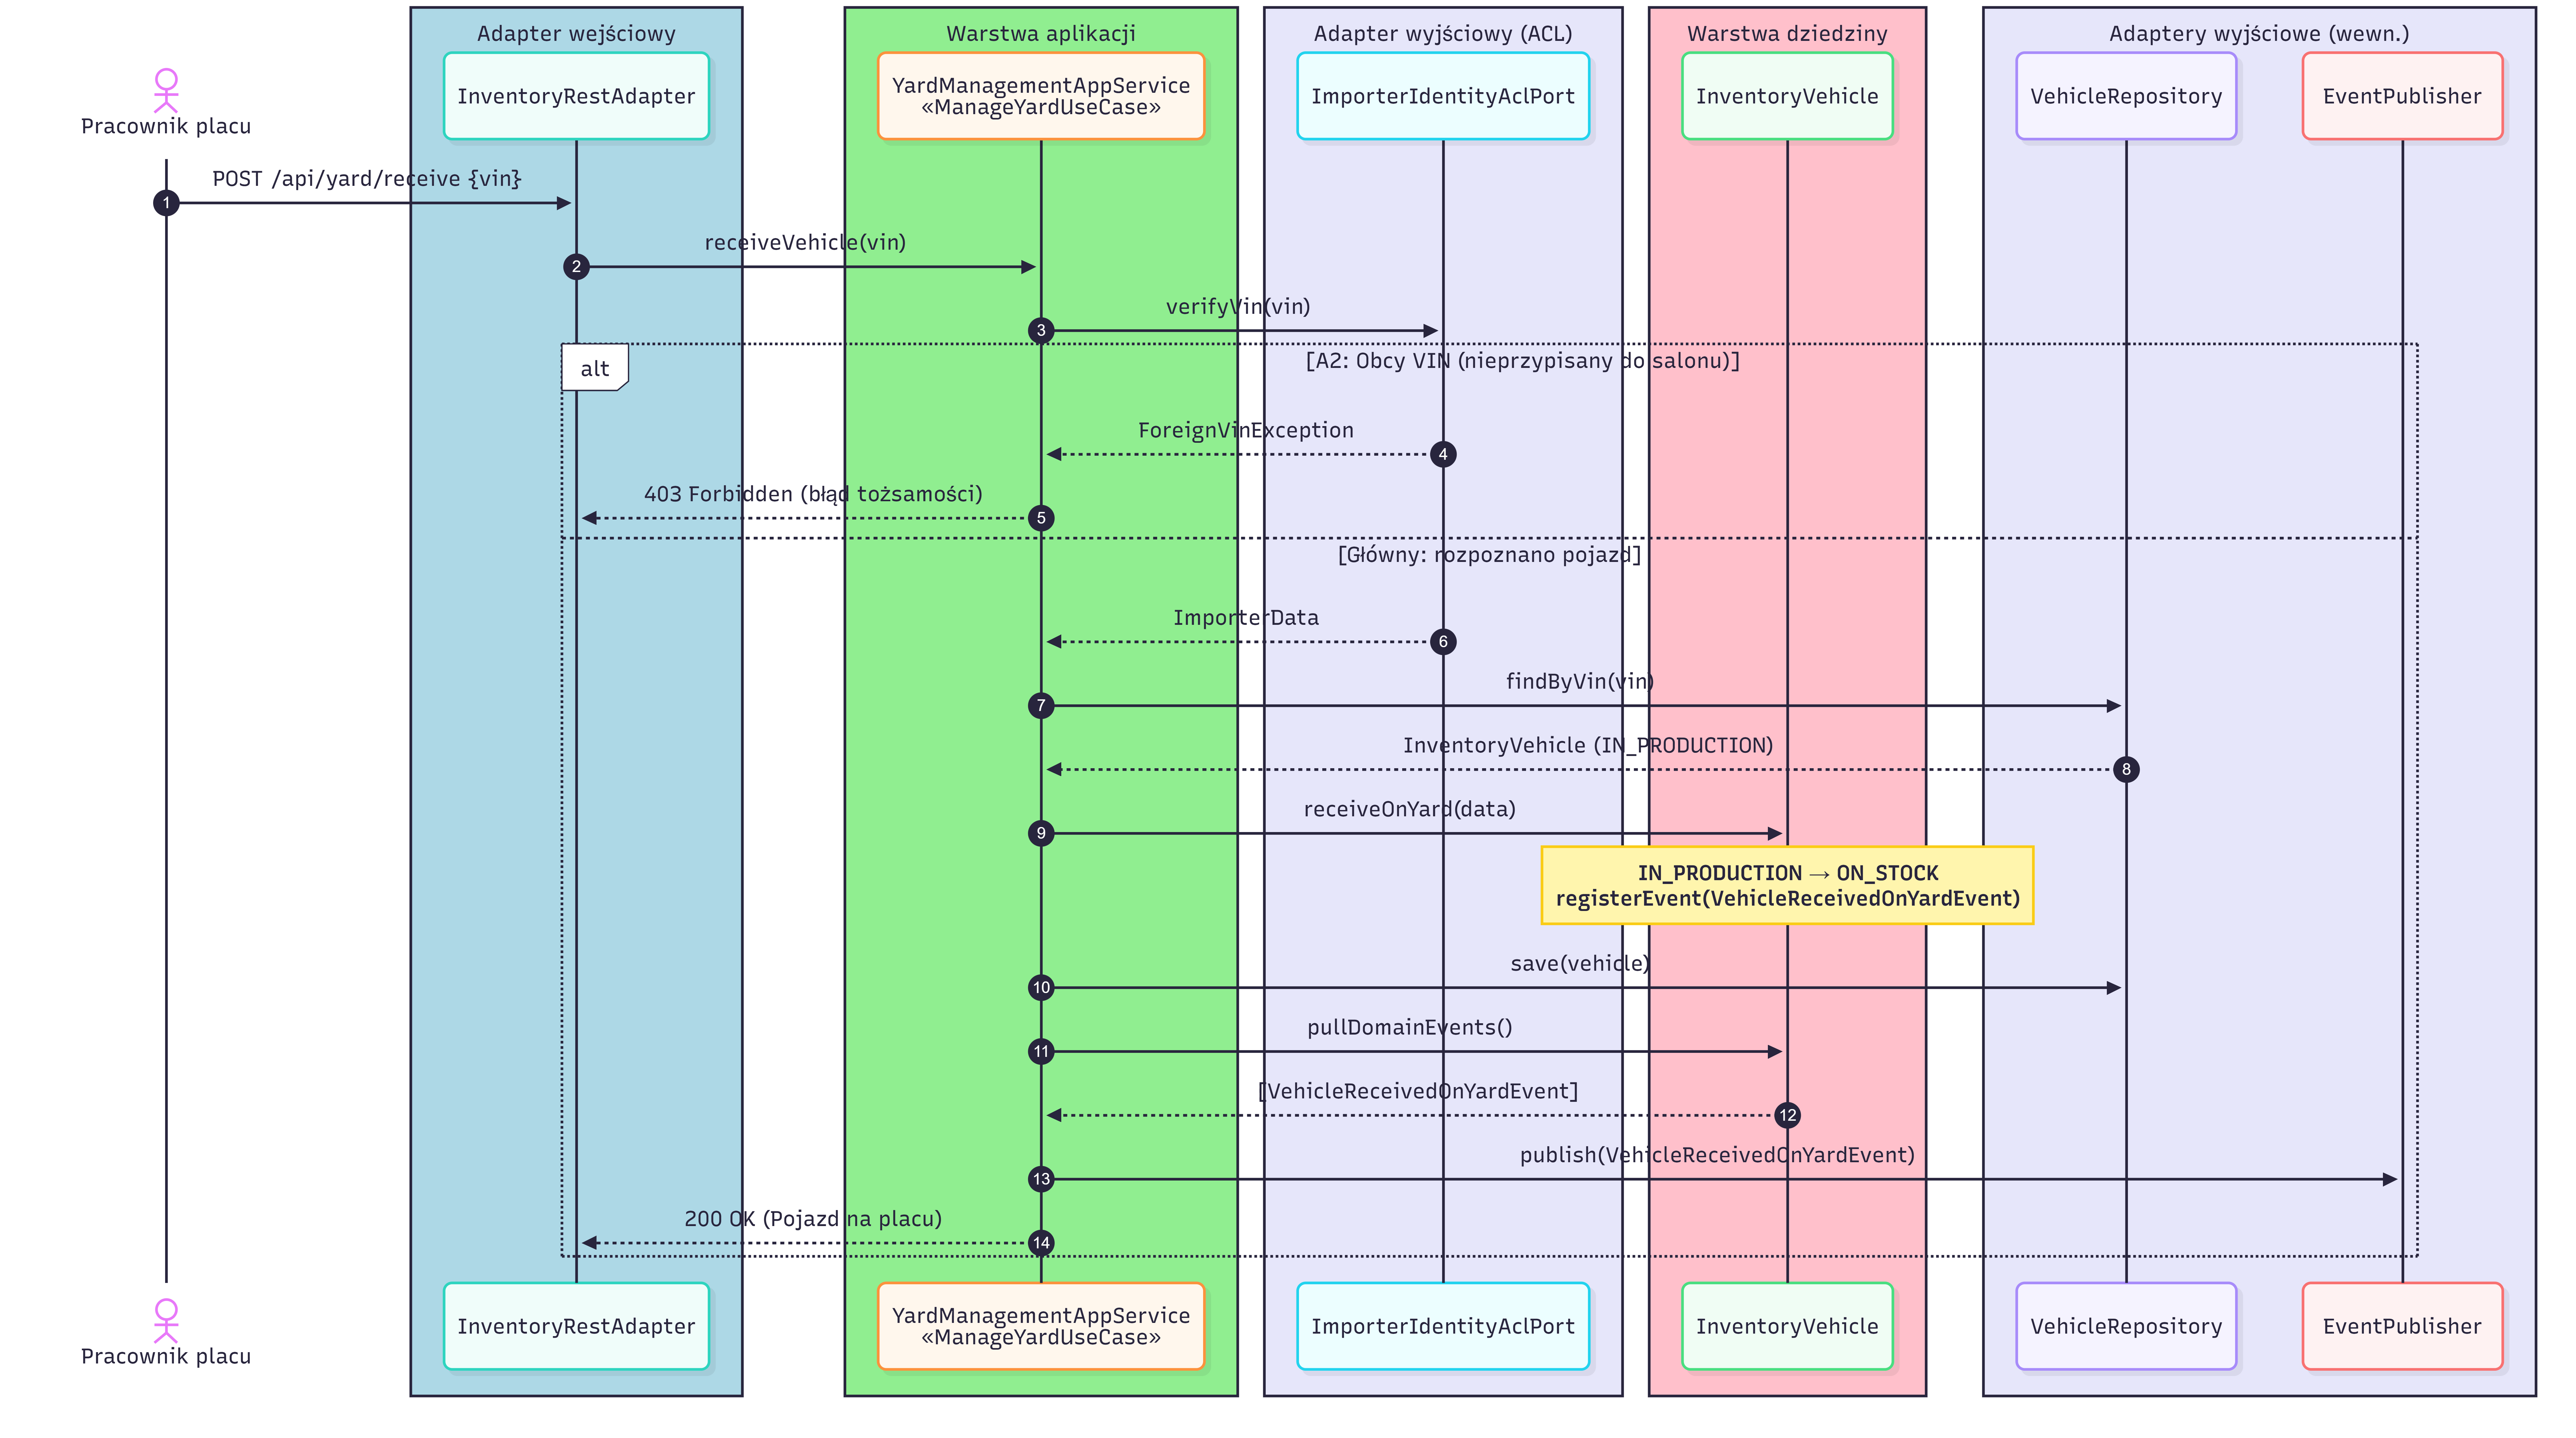
\includegraphics[width=1\textwidth]{media/diagramy_sekwencji/kontekst-inwentarza-logistyki/UC-INW-01-Sekwencji.png}
    \caption{Diagram sekwencji dla przypadku użycia UC-INW-01: Weryfikacja dostępności i rezerwacja pojazdu z placu}
    \label{fig:seq_uc_inw_01}
\end{figure}

% =====================================================
\textbf{UC-INW-02: Zlecenie produkcji pojazdu w fabryce}

\begin{longtable}{|p{4cm}|p{11cm}|}
\hline
\textbf{Element} & \textbf{Opis} \\
\hline

Identyfikator & UC-INW-02 \\
\hline

Nazwa & Zlecenie produkcji pojazdu w fabryce \\
\hline

Opis & 
Zautomatyzowane wysłanie zlecenia produkcji do systemu zewnętrznego fabryki/importera po opłaceniu wymaganego zadatku przez klienta. \\
\hline

Aktor główny & System (Kontekst Inwentarza i Logistyki) \\
\hline

Aktorzy pomocniczy & System zewnętrzny (API Importera) \\
\hline

Warunki wstępne & 
Samochód o określonej specyfikacji nie znajduje się na stanie magazynowym salonu samochodowego. Kontekst otrzymał zdarzenie z \textit{AdvancePaymentRegistered}. \\
\hline

Warunki końcowe & 
Zamówienie produkcyjne zostaje wysłane, a system emituje zdarzenie \textit{FactoryOrderPlacedEvent}. \\
\hline

Scenariusz główny & 
\begin{enumerate}
    \item System reaguje na zdarzenie o opłaceniu zadatku.
    \item System generuje żądanie produkcyjne na podstawie zatwierdzonej specyfikacji.
    \item System komunikuje się z API Importera/Fabryki i wysyła zlecenie.
    \item System oznacza to zamówienie lokalnie statusem "W produkcji".
    \item Kontekst emituje zdarzenie \textit{FactoryOrderPlacedEvent}.
\end{enumerate} \\
\hline

Scenariusze alternatywne & 
\begin{itemize}
    \item [A1] Fabryka odrzuca zlecenie: W kroku 3 API fabryki zwraca błąd (np. problem z połączeniem). System emituje zdarzenie \textit{FactoryOrderFailed}.
\end{itemize} \\
\hline
\end{longtable}

\begin{figure}[H]
    \centering
    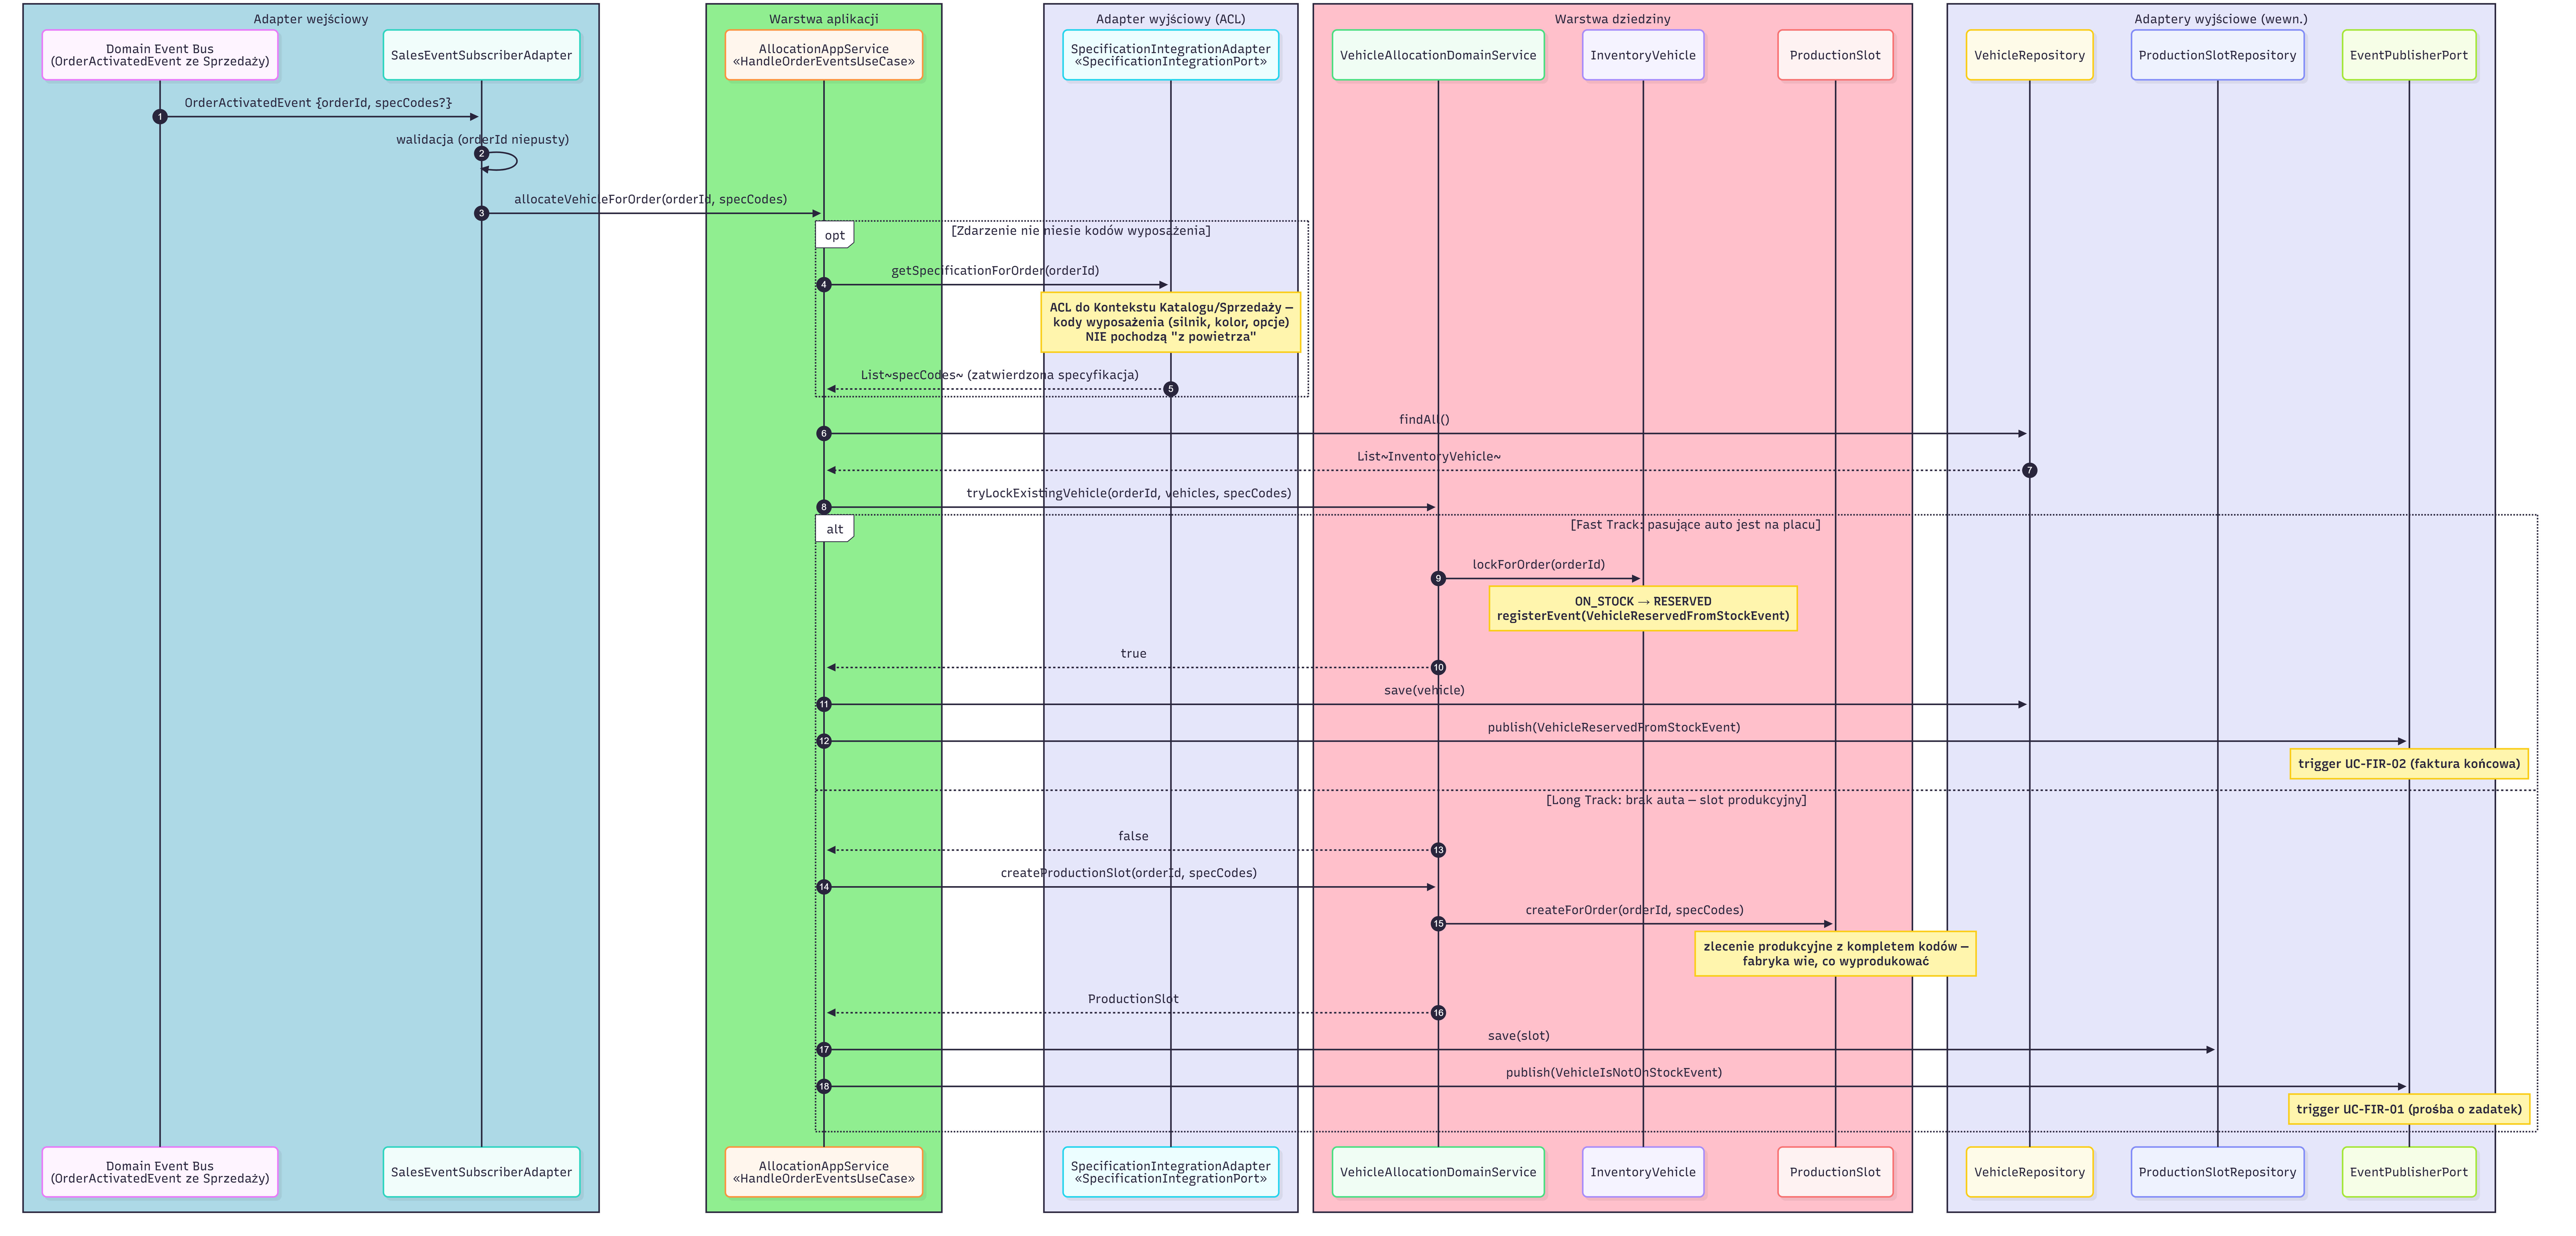
\includegraphics[width=1\textwidth]{media/diagramy_sekwencji/kontekst-inwentarza-logistyki/UC-INW-02-Sekwencji.png}
    \caption{Diagram sekwencji dla przypadku użycia UC-INW-02: Zlecenie produkcji pojazdu w fabryce}
    \label{fig:seq_uc_inw_02}
\end{figure}

% =====================================================
\textbf{UC-INW-03: Przyjęcie pojazdu na stan magazynowy}

\begin{longtable}{|p{4cm}|p{11cm}|}
\hline
\textbf{Element} & \textbf{Opis} \\
\hline

Identyfikator & UC-INW-03 \\
\hline

Nazwa & Przyjęcie pojazdu na stan magazynowy \\
\hline

Opis & 
Rejestracja fizycznego pojazdu, który przyjechał z fabryki na plac dealera, oraz powiązanie jego numeru VIN z oczekującym zamówieniem. \\
\hline

Aktor główny & Pracownik Placu (lub System Logistyczny Importera) \\
\hline

Aktorzy pomocniczy & - \\
\hline

Warunki wstępne & 
Fizyczny pojazd dotarł na plac salonu samochodowego. W systemie istnieje zamówienie o statusie "W produkcji". \\
\hline

Warunki końcowe & 
Pojazd jest zarejestrowany na stanie, otrzymuje status "Zarezerwowany" (przypisany do klienta), a system emituje zdarzenie \textit{VehicleDeliveredToStock}. \\
\hline

Scenariusz główny & 
\begin{enumerate}
    \item Pracownik placu rejestruje zjazd auta z lawety (skanując VIN).
    \item System tworzy nową kartotekę pojazdu w lokalnym inwentarzu.
    \item System automatycznie paruje ten numer VIN z oczekującym zamówieniem klienta.
    \item System zmienia status pojazdu na "Zarezerwowany".
    \item Kontekst emituje zdarzenie \textit{VehicleDeliveredToStock}.
\end{enumerate} \\
\hline

Scenariusze alternatywne & 
\begin{itemize}
    \item [A1] Auto nieprzypisane: W kroku 3 system nie znajduje zamówienia dla danej specyfikacji (np. auto zamówione "na stock"). Pojazd otrzymuje status "Wolny". Zdarzenie końcowe \textit{VehicleDeliveredToStock} nie jest emitowane.
\end{itemize} \\
\hline
\end{longtable}

\begin{figure}[H]
    \centering
    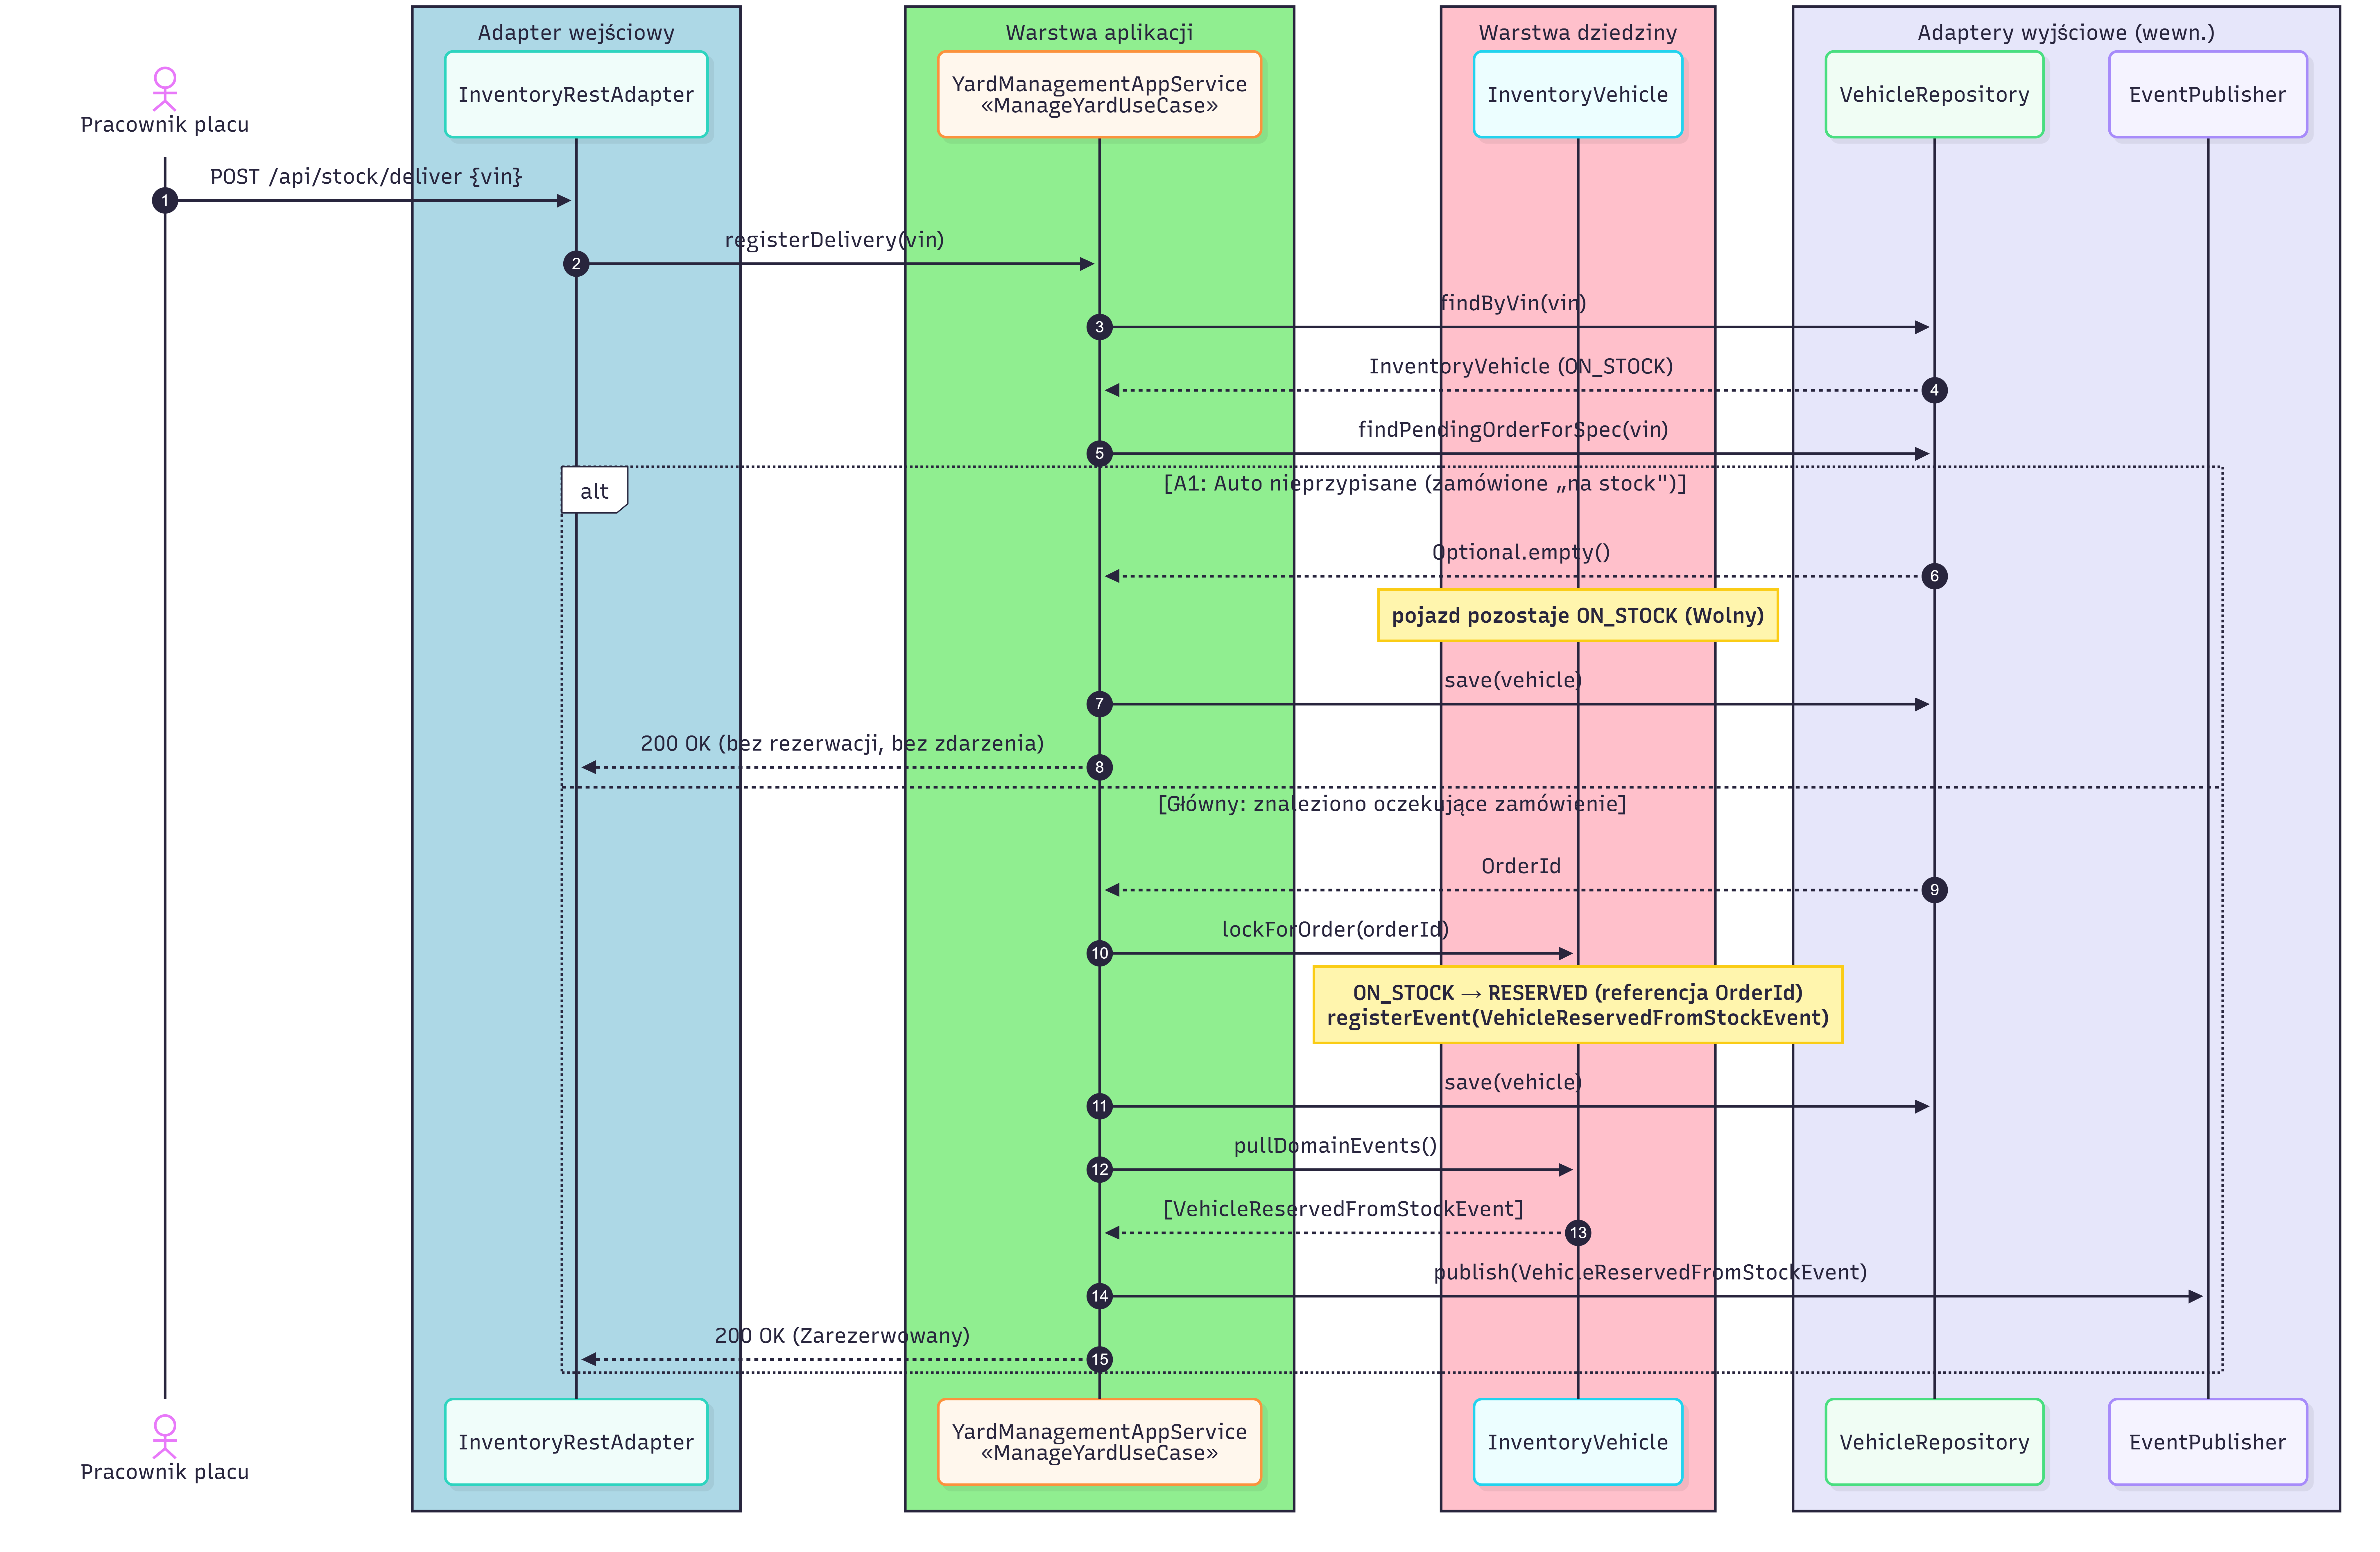
\includegraphics[width=1\textwidth]{media/diagramy_sekwencji/kontekst-inwentarza-logistyki/UC-INW-03-Sekwencji.png}
    \caption{Diagram sekwencji dla przypadku użycia UC-INW-03: Przyjęcie pojazdu na stan magazynowy}
    \label{fig:seq_uc_inw_03}
\end{figure}

% =====================================================
\textbf{UC-INW-04: Zwolnienie blokady pojazdu}

\begin{longtable}{|p{4cm}|p{11cm}|}
\hline
\textbf{Element} & \textbf{Opis} \\
\hline

Identyfikator & UC-INW-04 \\
\hline

Nazwa & Zwolnienie blokady pojazdu \\
\hline

Opis & 
Automatyczne zdjęcie rezerwacji z numeru VIN w przypadku braku uregulowania płatności końcowej w wyznaczonym terminie. \\
\hline

Aktor główny & System (Kontekst Inwentarza i Logistyki) \\
\hline

Aktorzy pomocniczy & - \\
\hline

Warunki wstępne & 
Kontekst otrzymał zdarzenie \textit{PaymentDeadlineExpired}. \\
\hline

Warunki końcowe & 
Pojazd wraca na plac do ponownej sprzedaży, emitowane jest zdarzenie \textit{VehicleReservationCancelledEvent}. \\
\hline

Scenariusz główny & 
\begin{enumerate}
    \item System reaguje na zdarzenie \textit{PaymentDeadlineExpired}.
    \item System wyszukuje numer VIN zablokowany dla tego zamówienia.
    \item System usuwa powiązanie VIN z zamówieniem i zmienia status pojazdu na "Wolny".
    \item Kontekst emituje zdarzenie \textit{VehicleReservationCancelledEvent}.
\end{enumerate} \\
\hline

Scenariusze alternatywne & 
\begin{itemize}
    \item [A1] Pojazd nie istnieje w rezerwacjach: Zablokowany pojazd został wcześniej usunięty/wydany.
\end{itemize} \\
\hline
\end{longtable}

\begin{figure}[H]
    \centering
    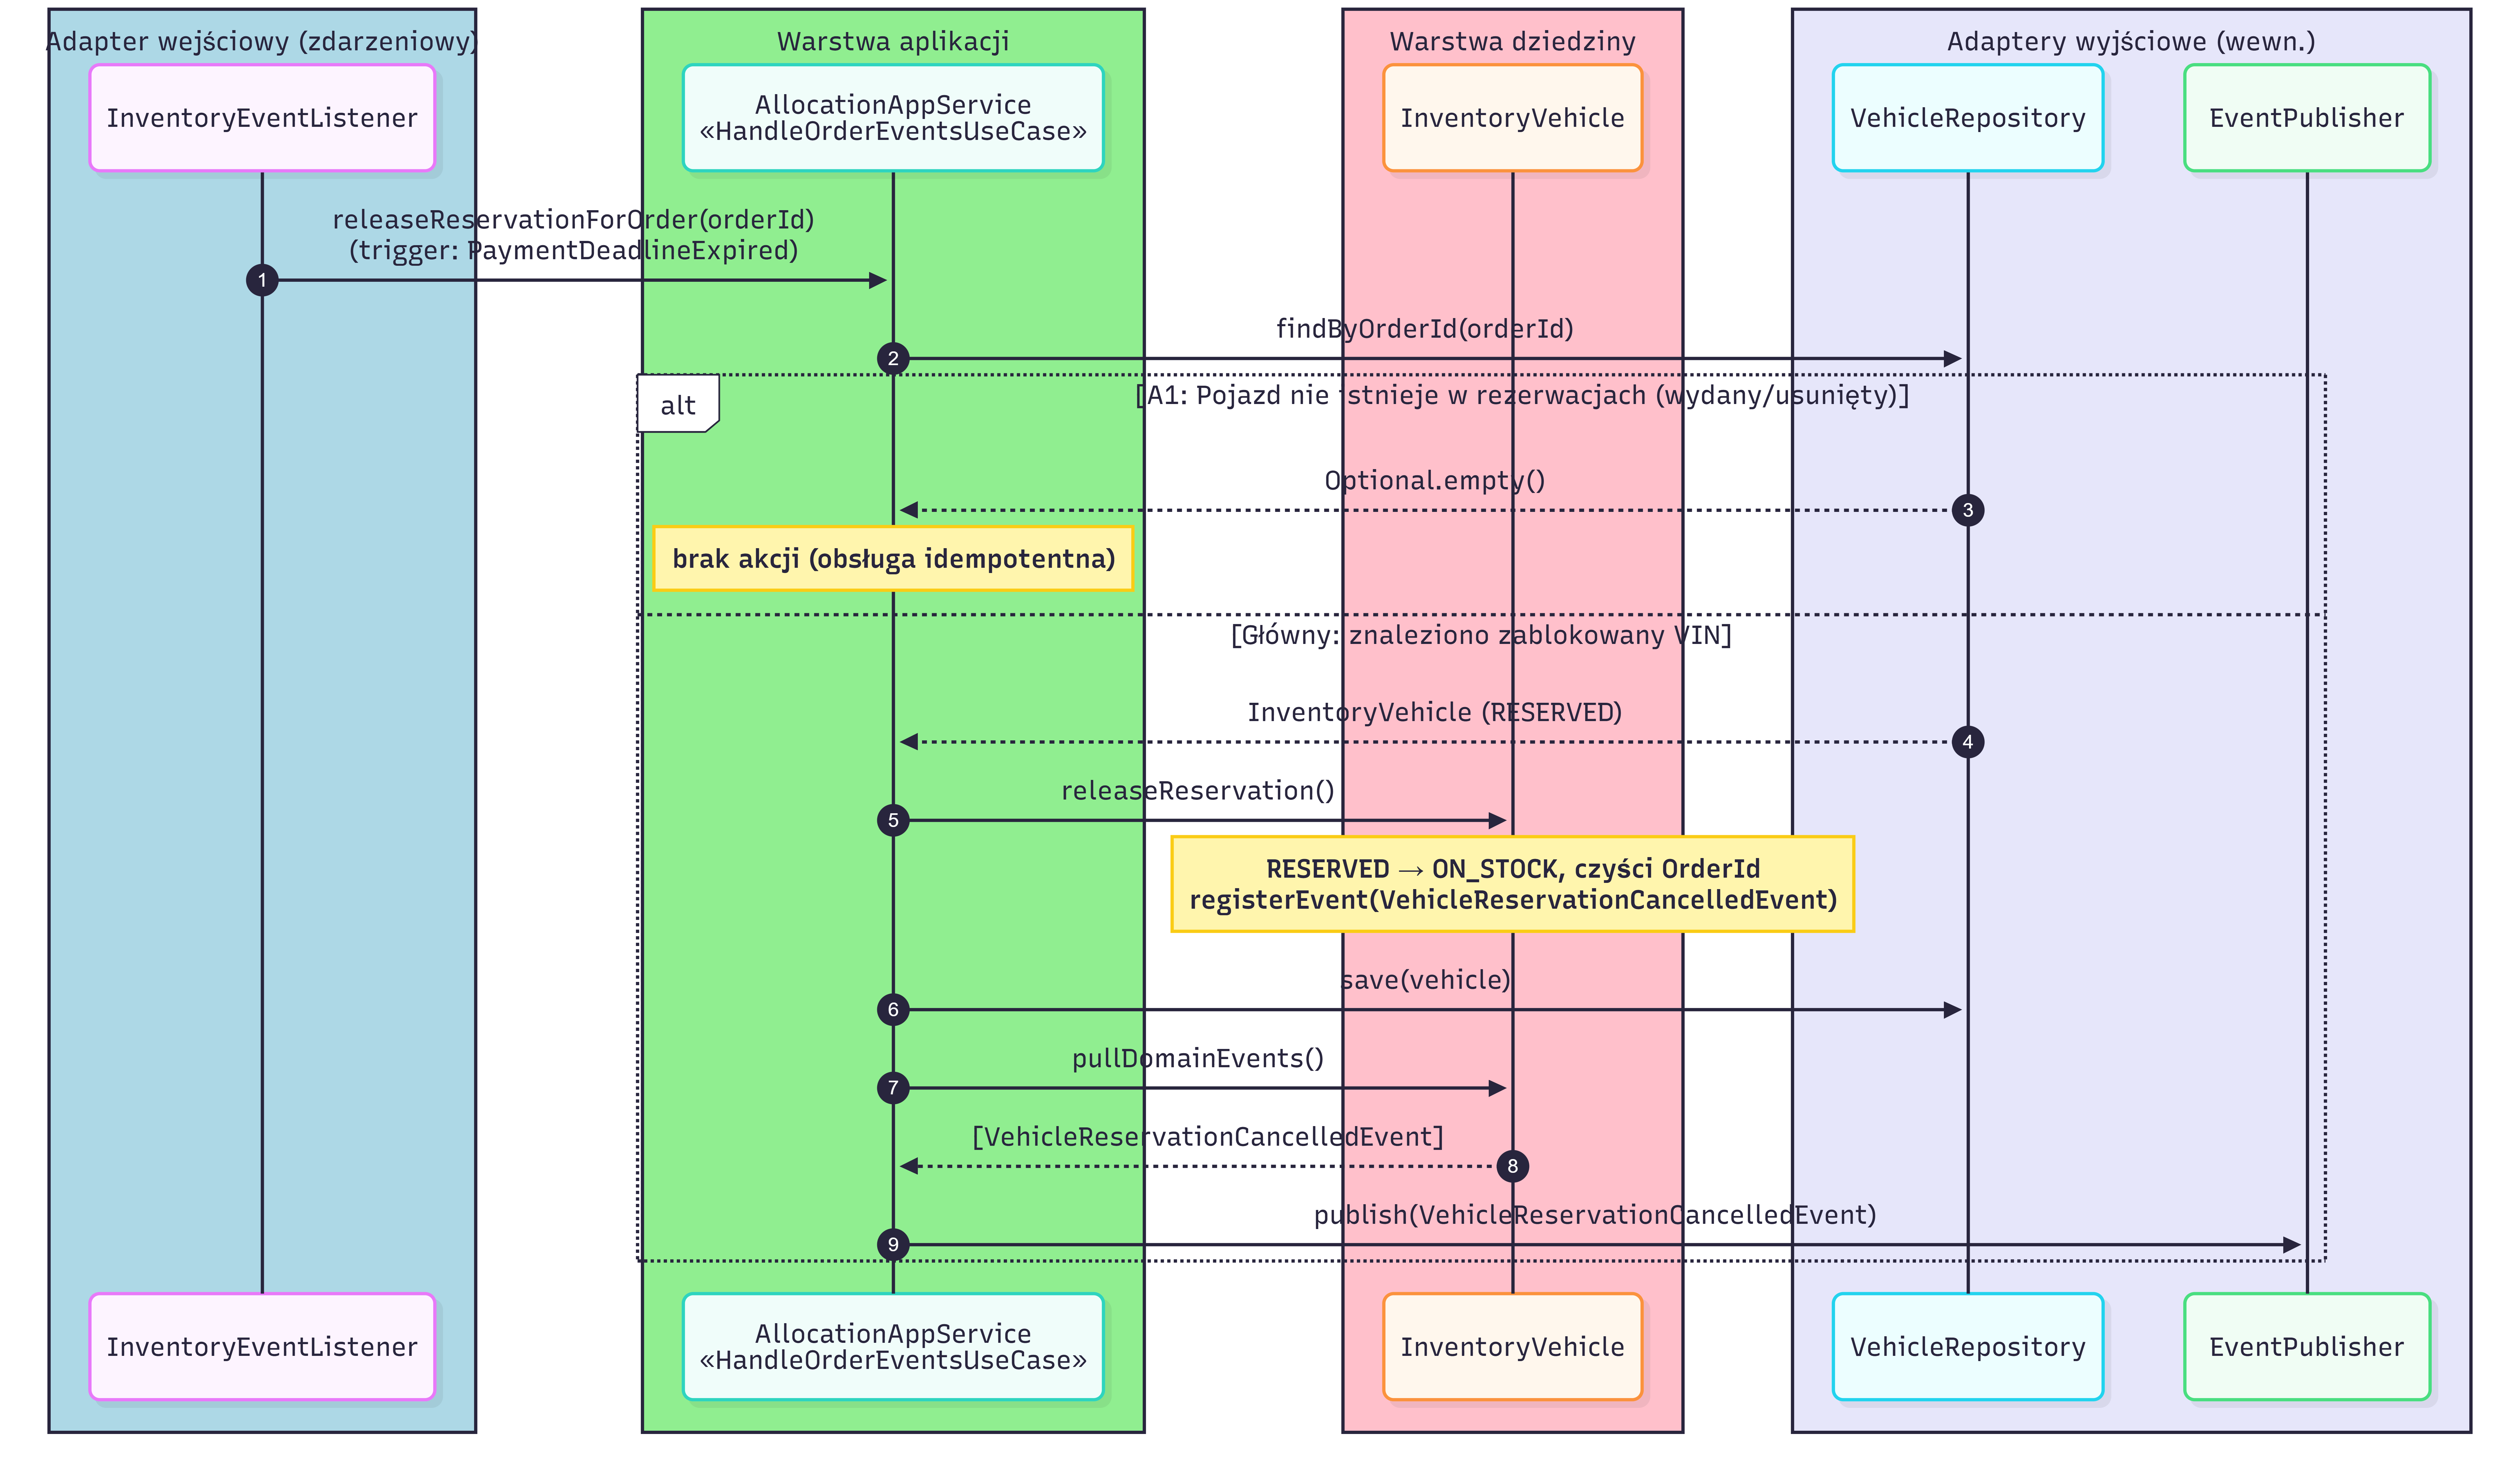
\includegraphics[width=1\textwidth]{media/diagramy_sekwencji/kontekst-inwentarza-logistyki/UC-INW-04-Sekwencji.png}
    \caption{Diagram sekwencji dla przypadku użycia UC-INW-04: Zwolnienie blokady pojazdu}
    \label{fig:seq_uc_inw_04}
\end{figure}

% =====================================================
\textbf{UC-INW-05: Przygotowanie pojazdu do wydania po rozliczeniu}

\begin{longtable}{|p{4cm}|p{11cm}|}
\hline
\textbf{Element} & \textbf{Opis} \\
\hline

Identyfikator & UC-INW-05 \\
\hline

Nazwa & Przygotowanie pojazdu do wydania po rozliczeniu \\
\hline

Opis & 
Systemowa zmiana statusu pojazdu na "Gotowy do wydania" po otrzymaniu potwierdzenia pełnego rozliczenia zamówienia. \\
\hline

Aktor główny & System (Kontekst Inwentarza) \\
\hline

Aktorzy pomocniczy & - \\
\hline

Warunki wstępne & 
Pojazd ma status 'Zarezerwowany', kontekst otrzymał zdarzenie \textit{SettlementCompleted}. \\
\hline

Warunki końcowe & 
Status pojazdu zmieniony na 'Gotowy do wydania', emitowane zdarzenie \textit{VehicleReadyForHandover}. \\
\hline

Scenariusz główny & 
\begin{enumerate}
    \item System reaguje na zdarzenie \textit{SettlementCompleted}.
    \item System weryfikuje, czy dla danego VIN-u istnieje aktywna rezerwacja.
    \item System zmienia status pojazdu z 'Zarezerwowany' na 'Gotowy do wydania'.
    \item Kontekst emituje zdarzenie \textit{VehicleReadyForHandoverEvent}.
\end{enumerate} \\
\hline

Scenariusze alternatywne & 
\begin{itemize}
    \item [] Brak.
\end{itemize} \\
\hline
\end{longtable}

\begin{figure}[H]
    \centering
    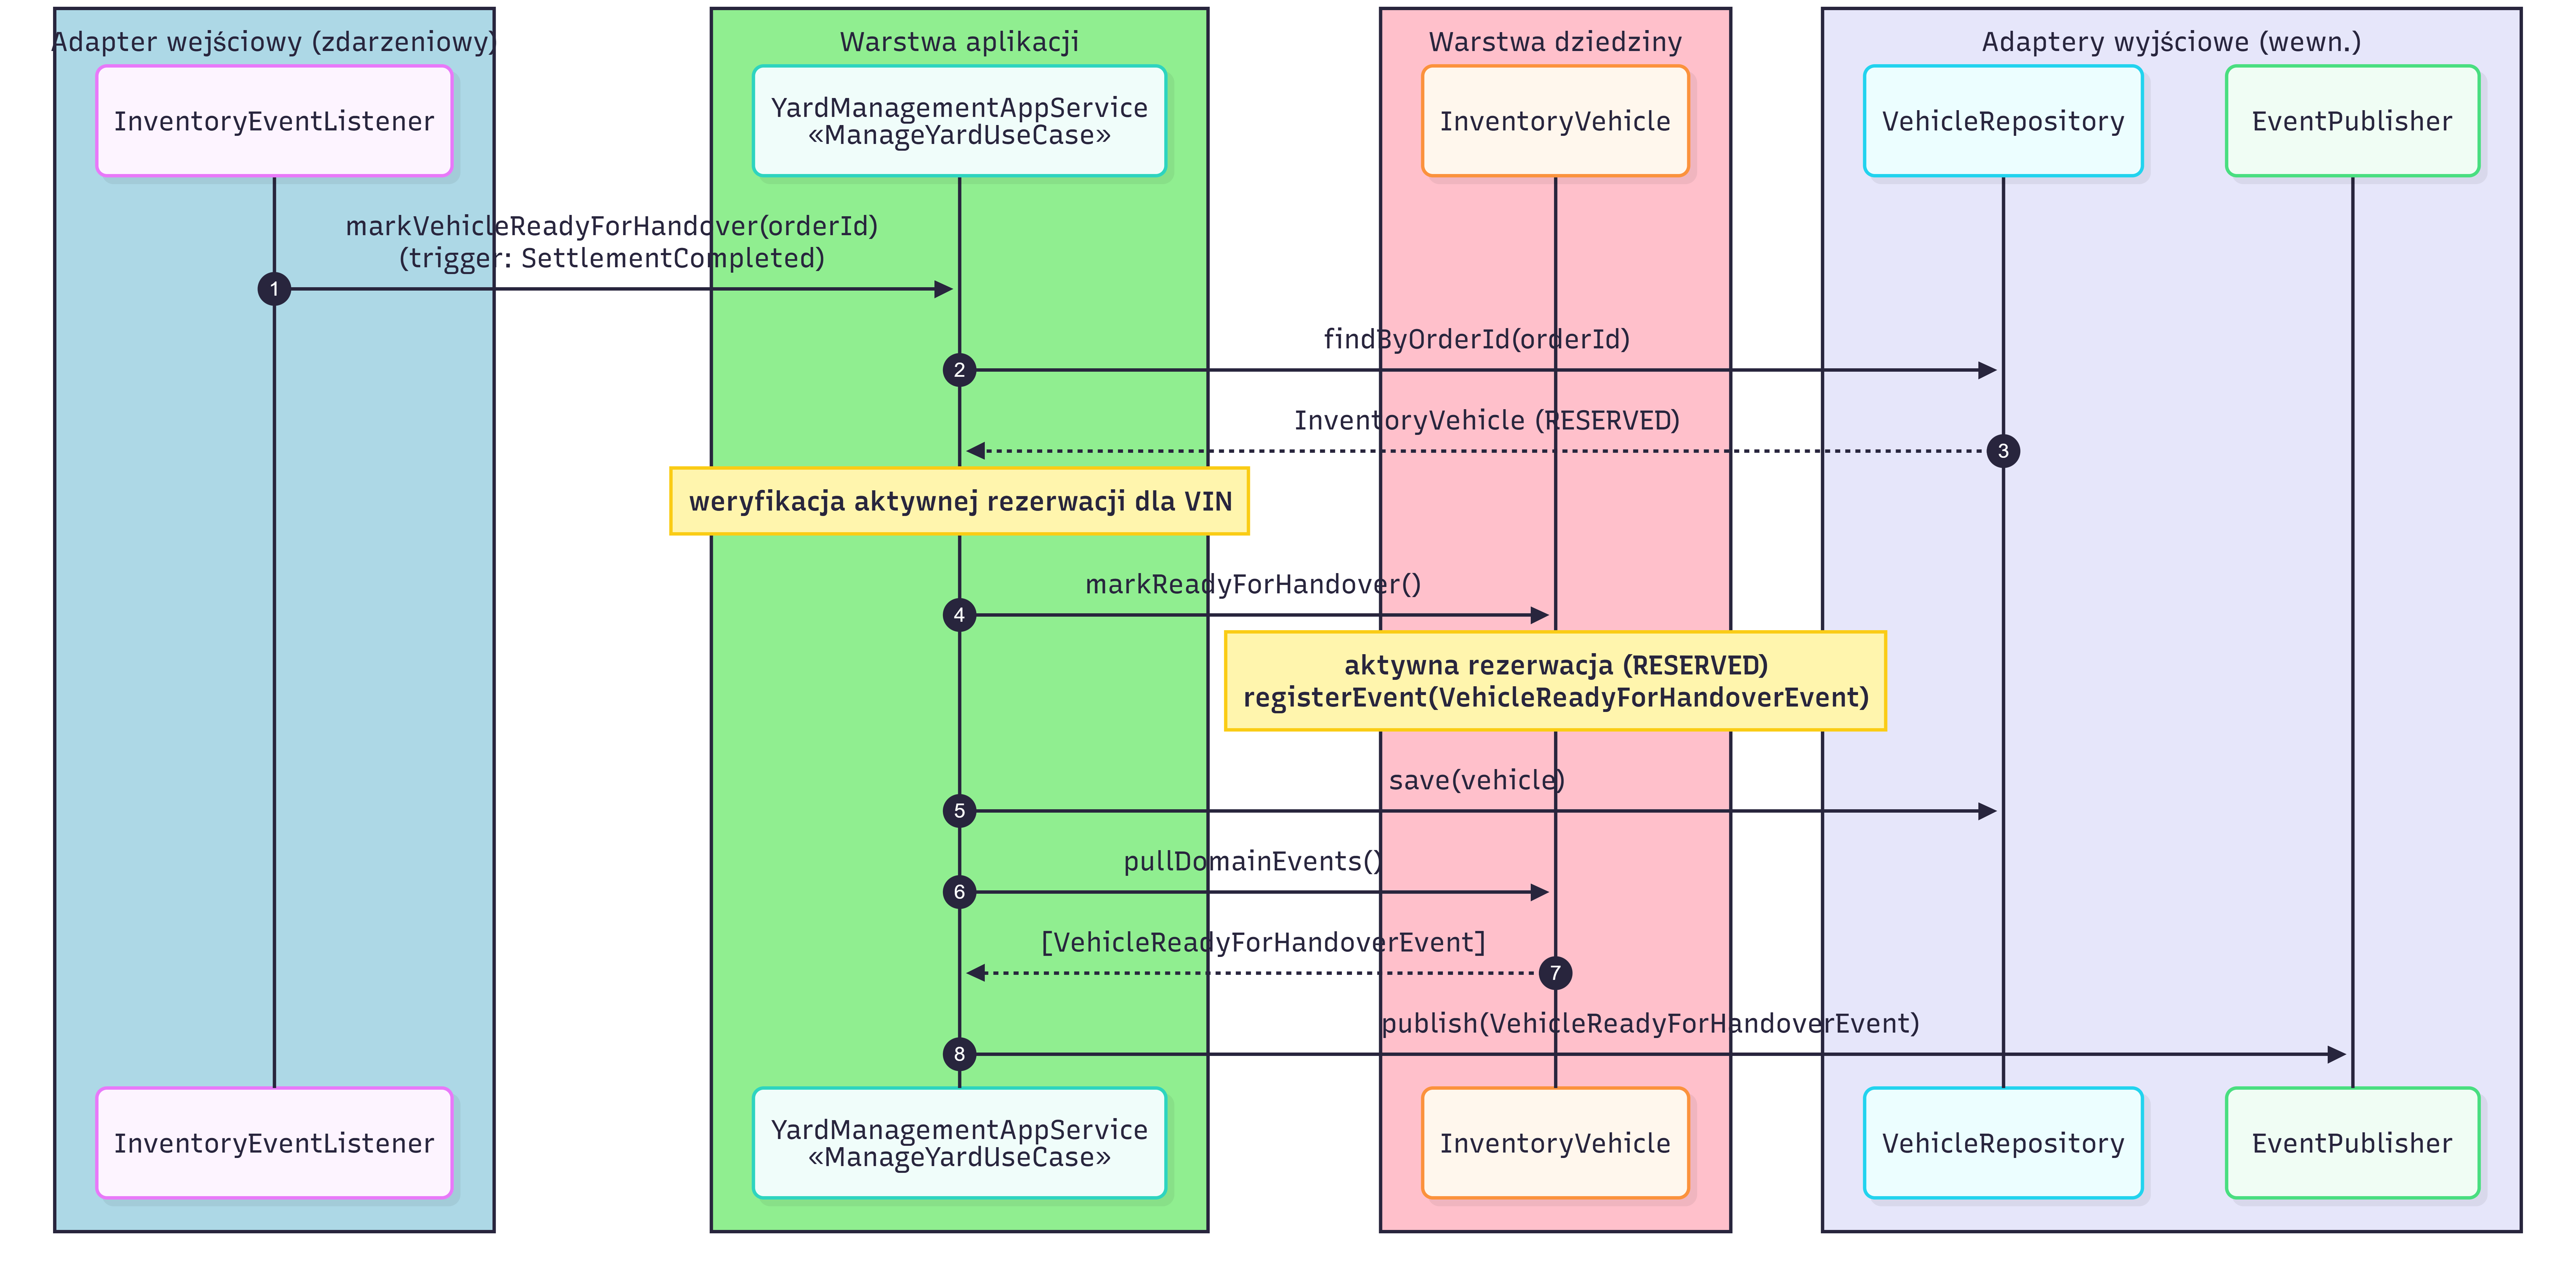
\includegraphics[width=1\textwidth]{media/diagramy_sekwencji/kontekst-inwentarza-logistyki/UC-INW-05-Sekwencji.png}
    \caption{Diagram sekwencji dla przypadku użycia UC-INW-05: Przygotowanie pojazdu do wydania po rozliczeniu}
    \label{fig:seq_uc_inw_05}
\end{figure}

% =====================================================
\textbf{UC-INW-06: Zdjęcie pojazdu ze stanu magazynowego}

\begin{longtable}{|p{4cm}|p{11cm}|}
\hline
\textbf{Element} & \textbf{Opis} \\
\hline

Identyfikator & UC-INW-06 \\
\hline

Nazwa & Zdjęcie pojazdu ze stanu magazynowego \\
\hline

Opis & 
Automatyczna operacja zmiany statusu pojazdu na "Wydany" w Inwentarzu, wywołana komendą z modułu Sprzedaży/CRM. \\
\hline

Aktor główny & System (Kontekst Inwentarza i Logistyki) \\
\hline

Aktorzy pomocniczy & - \\
\hline

Warunki wstępne & 
Pojazd ma status "Gotowy do wydania". Kontekst otrzymał komendę oznaczającą fizyczne wydanie auta \textit{ReleaseVehicle}. \\
\hline

Warunki końcowe & 
Status pojazdu zmieniony na "Wydany", emitowane zdarzenie \textit{VehicleInventoryReleased}. \\
\hline

Scenariusz główny & 
\begin{enumerate}
    \item System Inwentarza odbiera komendę \textit{ReleaseVehicle}.
    \item System weryfikuje status pojazdu pod kątem gotowości do wydania.
    \item System zdejmuje pojazd z aktywnego stanu magazynowego, zmieniając jego status na "Wydany".
    \item Kontekst emituje zdarzenie \textit{VehicleInventoryReleased}.
\end{enumerate} \\
\hline

Scenariusze alternatywne & 
\begin{itemize}
    \item [A1] Niewłaściwy status pojazdu: W kroku 2 pojazd ma status inny niż "Gotowy do wydania". System odrzuca komendę i emituje zdarzenie \textit{VehicleInventoryReleasedError}.
\end{itemize} \\
\hline
\end{longtable}

\begin{figure}[H]
    \centering
    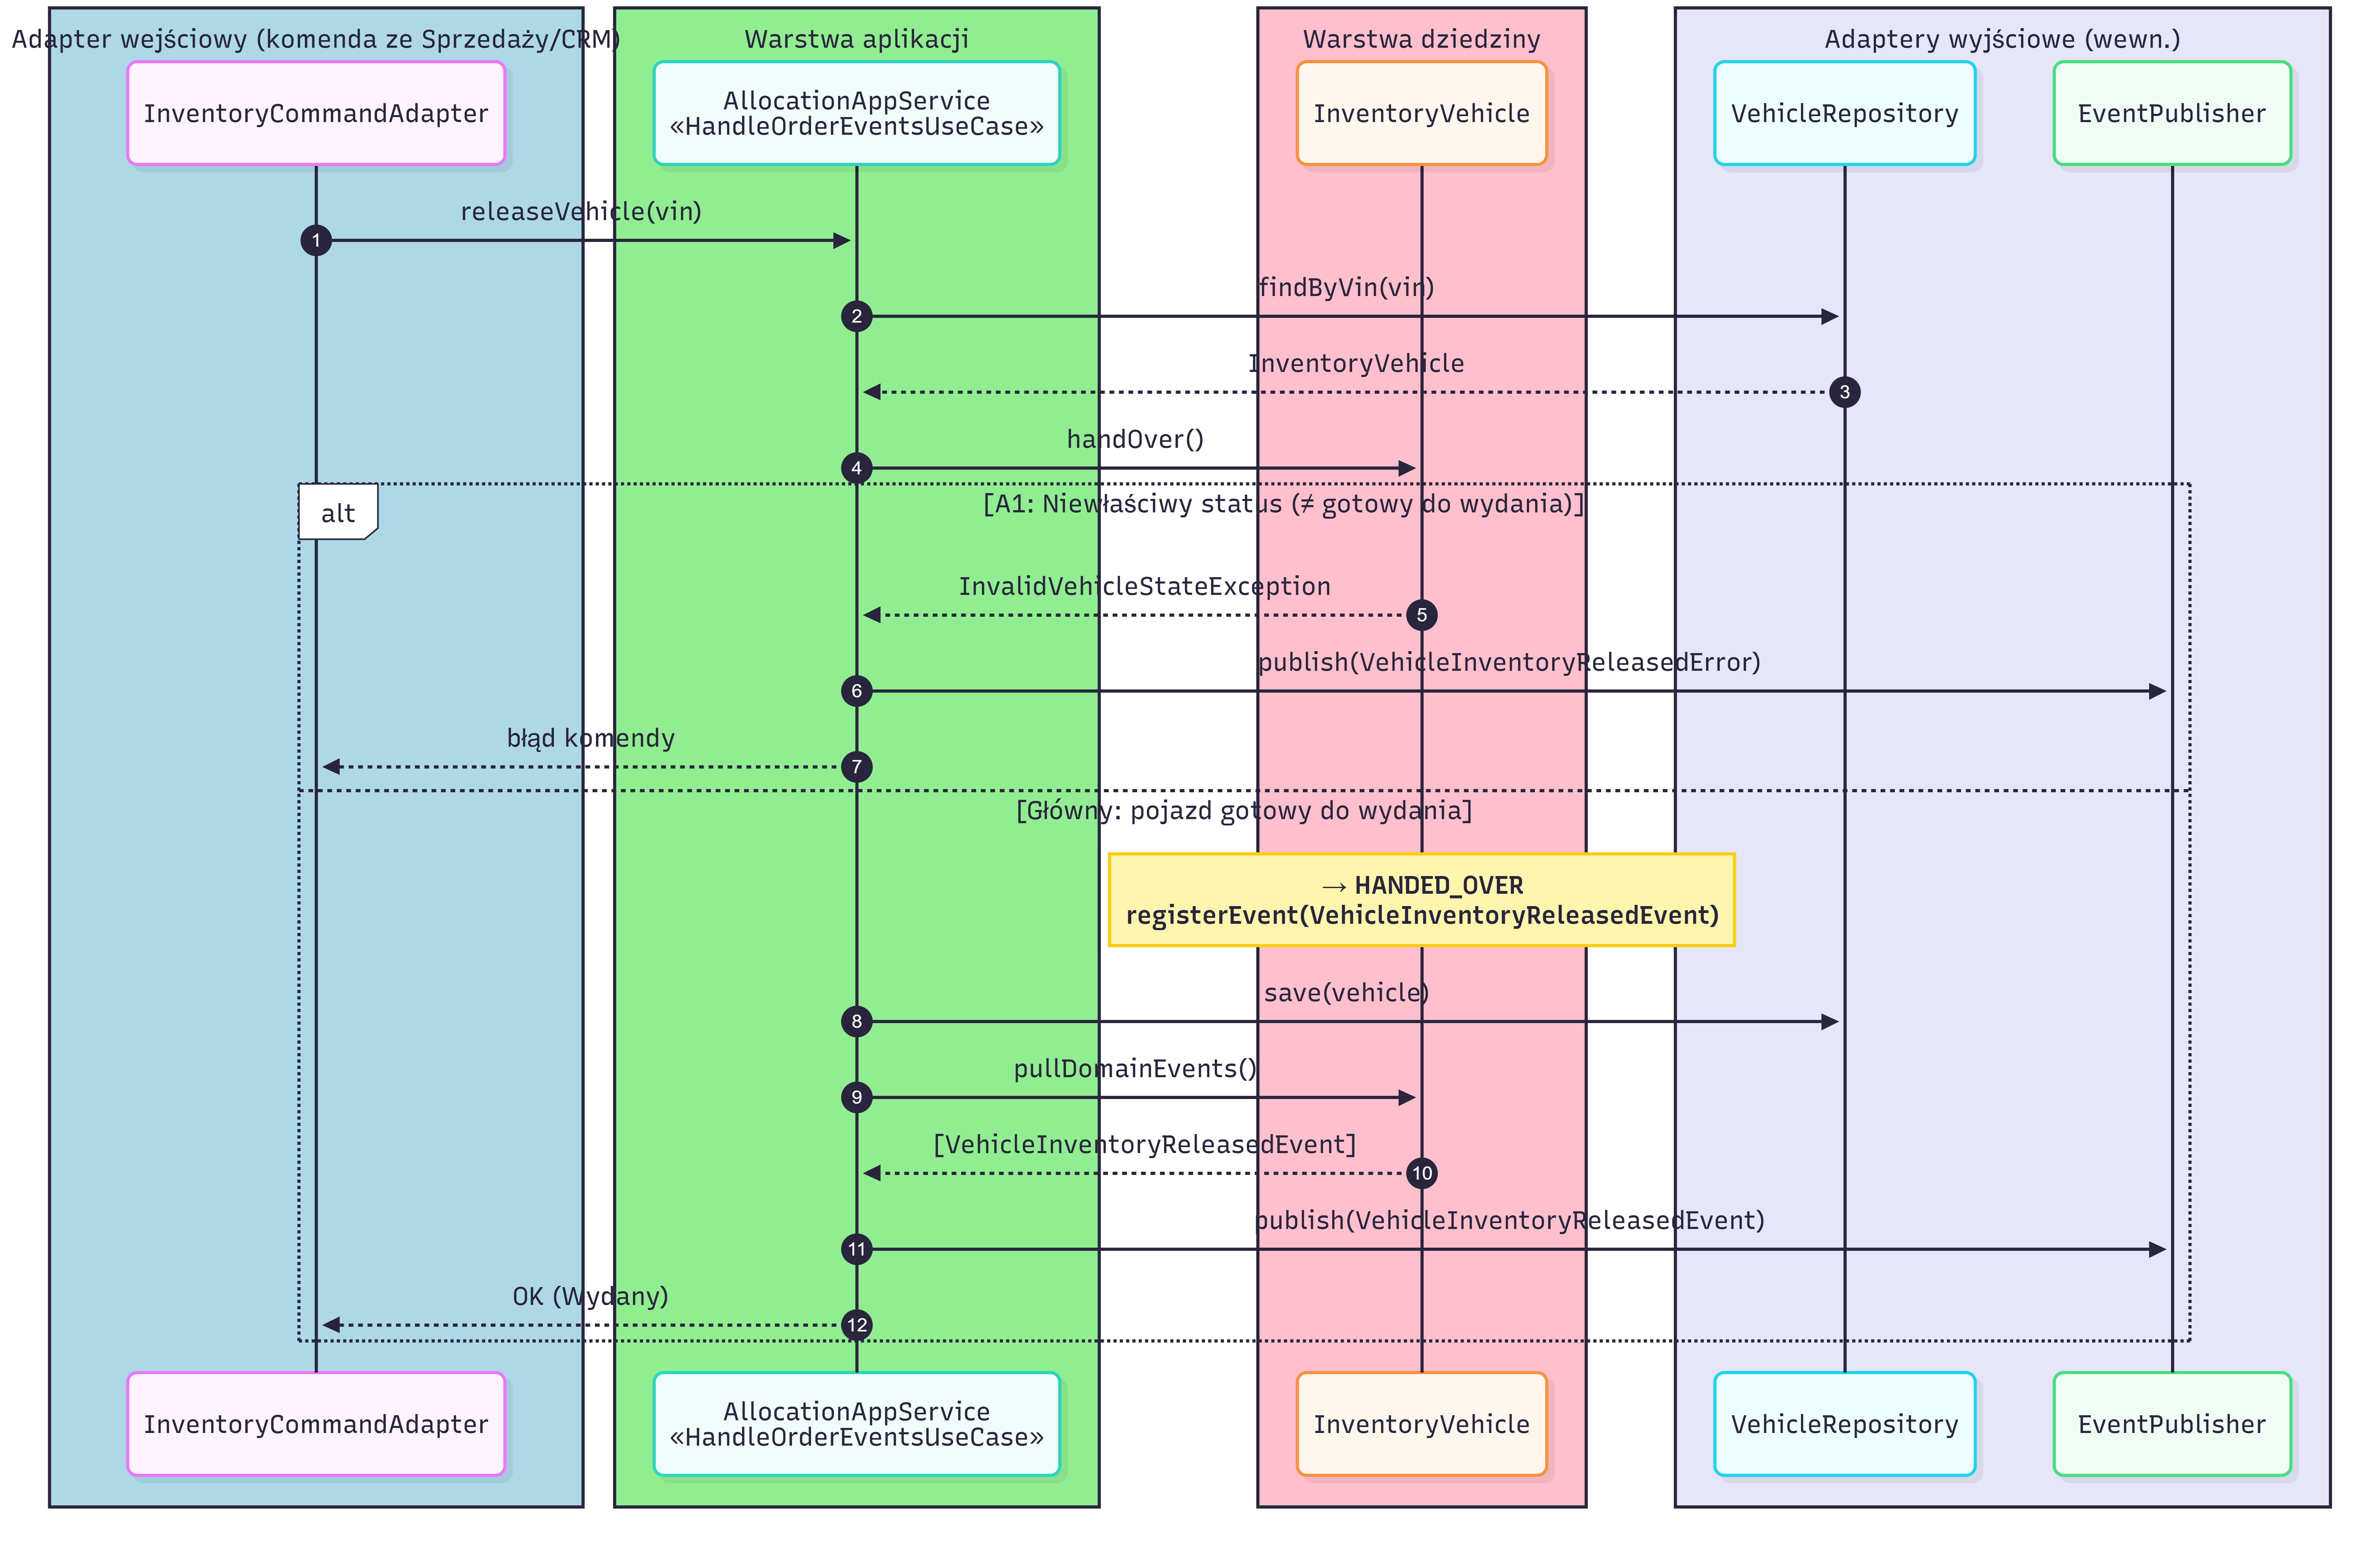
\includegraphics[width=1\textwidth]{media/diagramy_sekwencji/kontekst-inwentarza-logistyki/UC-INW-06-Sekwencji.png}
    \caption{Diagram sekwencji dla przypadku użycia UC-INW-06: Zdjęcie pojazdu ze stanu magazynowego}
    \label{fig:seq_uc_inw_06}
\end{figure}

\subsubsection{Architektura Kontekstu Inwentarza i Logistyki}

Kontekst Inwentarza i Logistyki został zaprojektowany w oparciu o architekturę heksagonalną. Diagram Architektury przedstawiono na rysunku \ref{fig:hex_logisics}.

\begin{figure}[H]
    \centering
    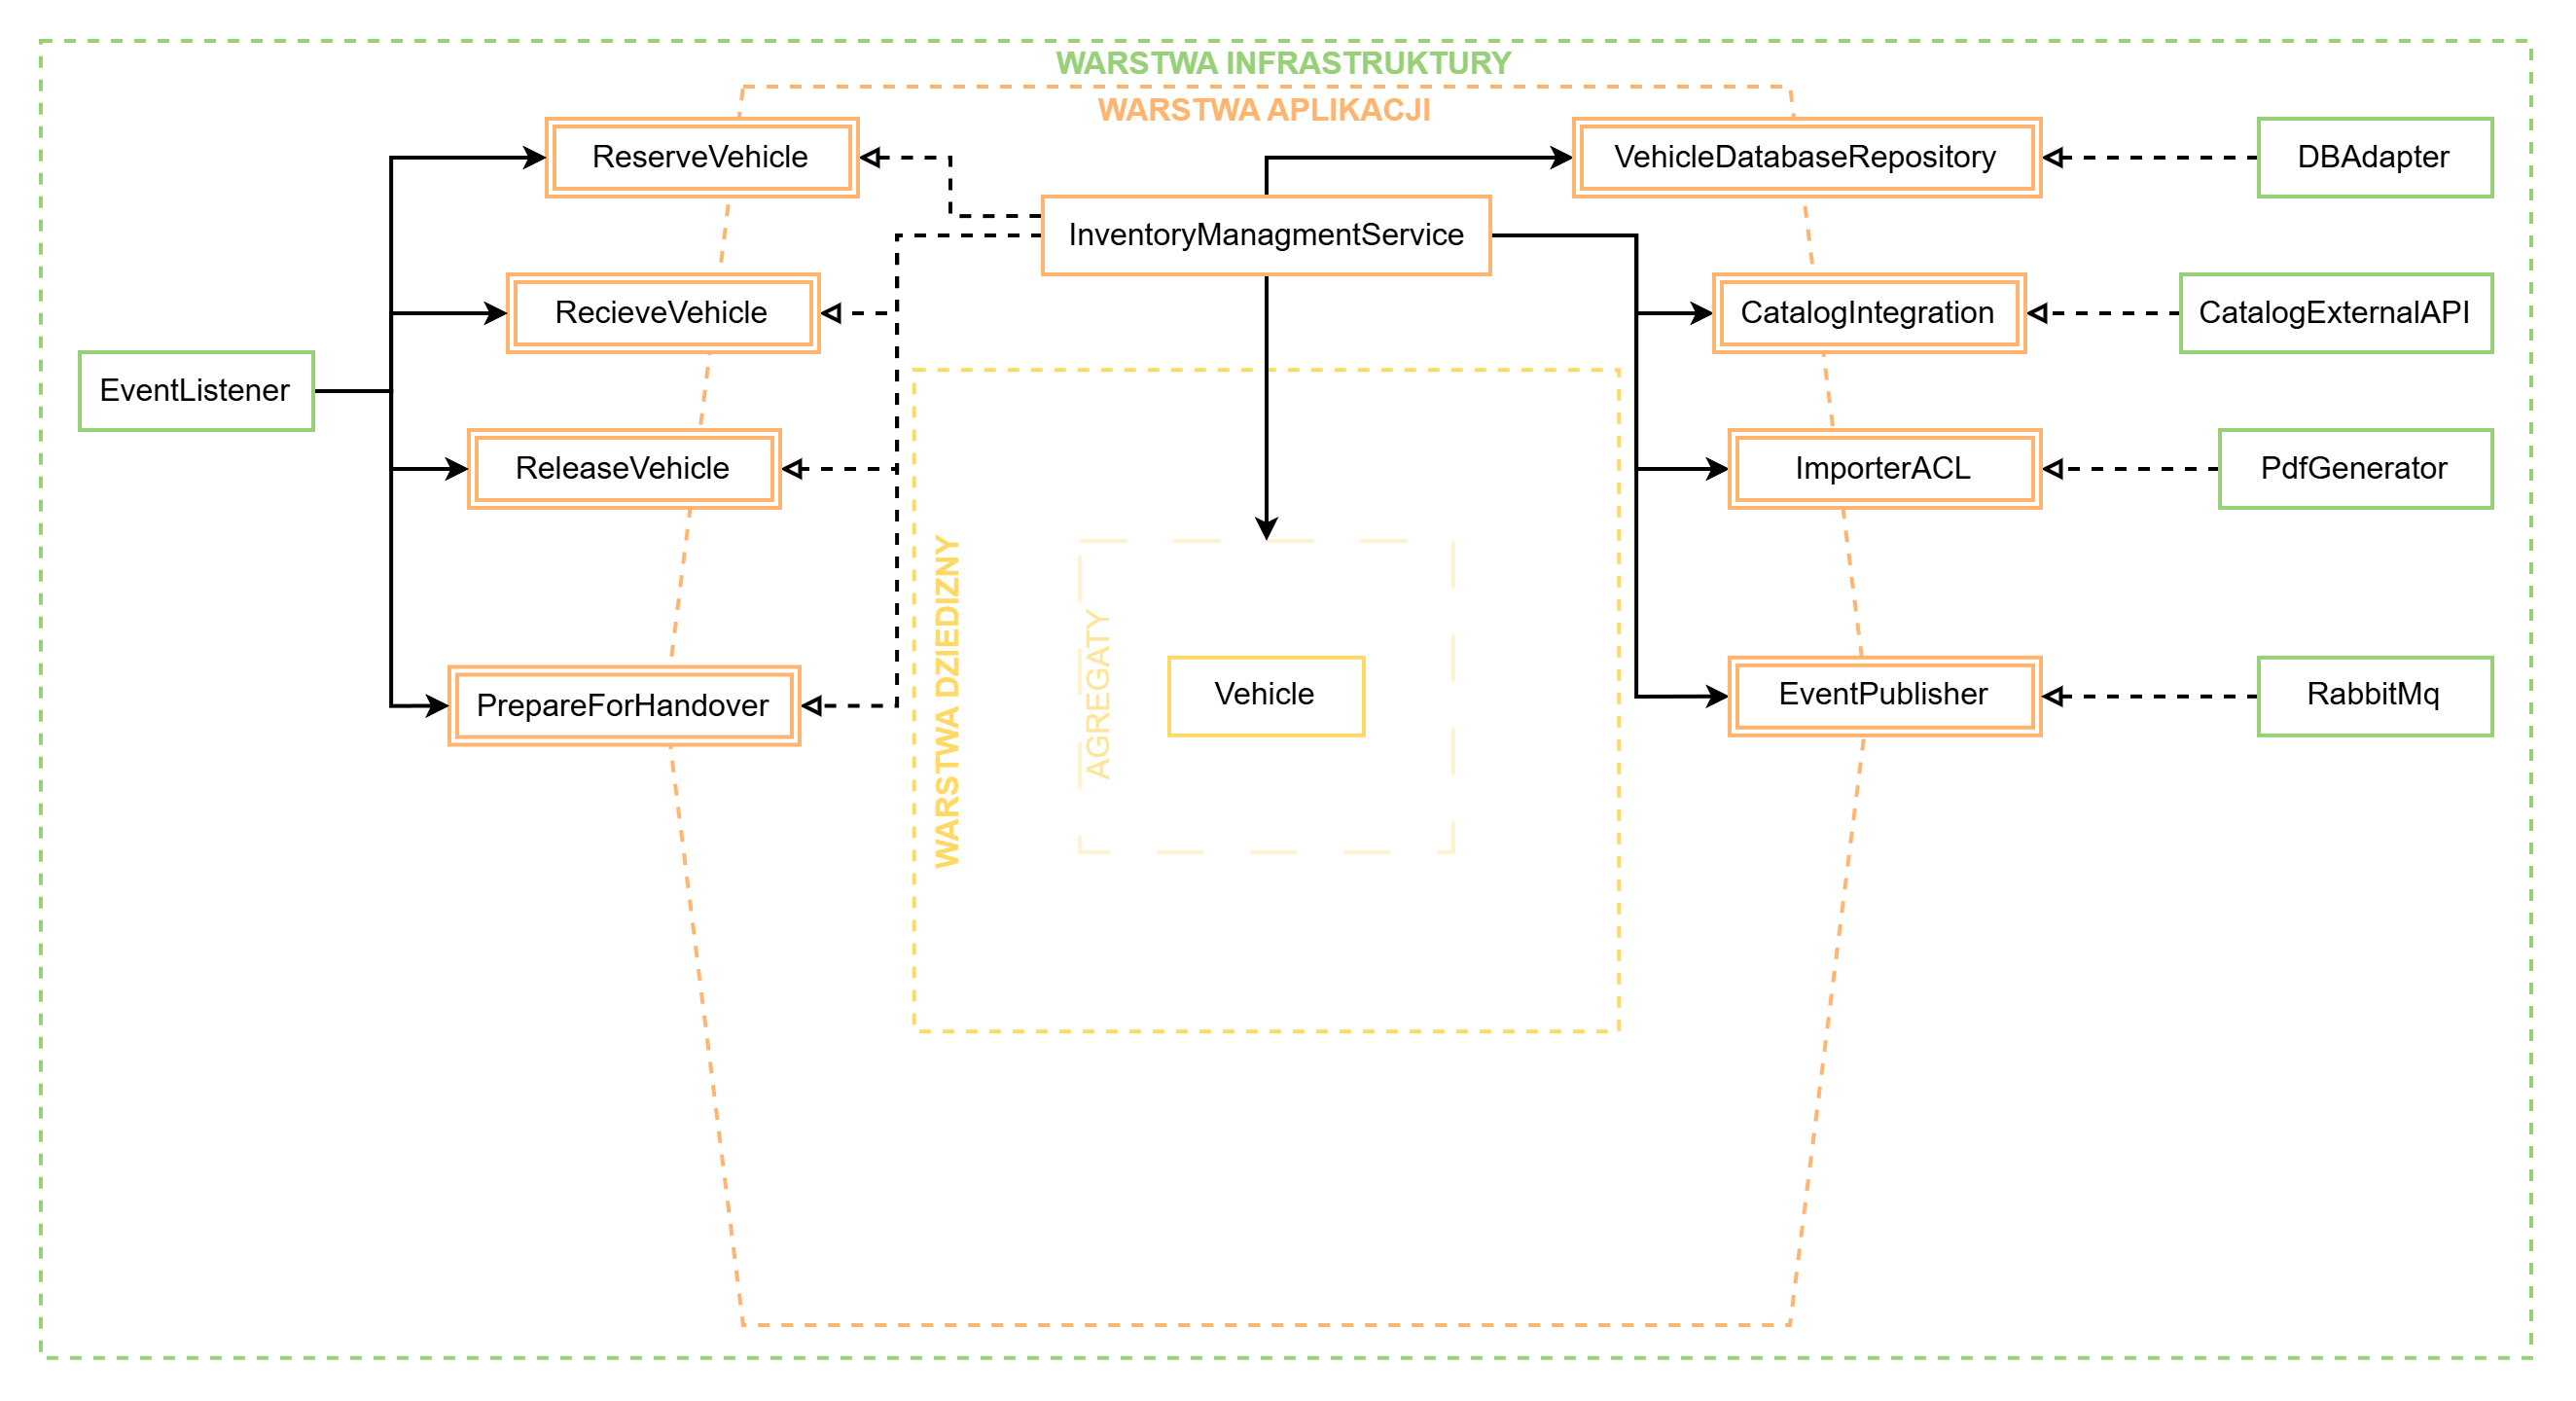
\includegraphics[width=1\linewidth]{media//architektura_heksagonalna/LogisticsArchitecture.png}
    \caption{Architektura heksagonalna kontekstu inwentarza i logistyki}
    \label{fig:hex_logisics}
\end{figure}

Poniżej przedstawiono szczegółowy opis interakcji pomiędzy warstwami, z podziałem na strony wejściową i wyjściową.

\paragraph{Strona Wejściowa: Porty i Adaptery} 
Ta strona heksagonu definiuje, w jaki sposób systemy zewnętrzne oraz operatorzy komunikują się z modułem logistyki w celu zmiany stanu magazynowego pojazdów.

Wszystkie cztery porty wejściowe realizowane są przez jedną scentralizowaną usługę \texttt{InventoryManagementService}.

\begin{itemize}
    \item \textbf{Rezerwacje i Produkcja (Asynchroniczne)}
    \begin{itemize}
        \item \textbf{Porty:} \texttt{ReserveVehicle} (UC-INW-01: rezerwacja z placu oraz UC-INW-02: zlecenie produkcji — \texttt{orderVehicleFromFactory}) i \texttt{ReleaseVehicle} (UC-INW-04: zwolnienie rezerwacji oraz UC-INW-06: zwolnienie pojazdu).
        \item \textbf{Adaptery (Messaging):} \texttt{SalesEventSubscriberAdapter} (zdarzenie \texttt{OrderPlaced} oraz komenda zwolnienia z Inwentarza), \texttt{BillingEventSubscriberAdapter} (\texttt{AdvancePaymentRegistered}~$\rightarrow$~zlecenie produkcji, \texttt{PaymentDeadlineExpired}~$\rightarrow$~zwolnienie rezerwacji), \texttt{FinancingEventSubscriberAdapter} (decyzja banku) oraz \texttt{CatalogEventSubscriberAdapter} (\texttt{SpecificationCompleted} zasilające lokalną kopię danych Katalogu).
    \end{itemize}

    \item \textbf{Obrót Magazynowy i Wydanie}
    \begin{itemize}
        \item \textbf{Porty:} \texttt{ReceiveVehicle} (UC-INW-03: przyjęcie pojazdu na plac) oraz \texttt{PrepareForHandover} (UC-INW-05: przygotowanie do wydania).
        \item \textbf{Adapter (HTTP):} \texttt{VehicleArrivalRestAdapter}. Udostępnia API dla pracowników placu, parsując żądania sieciowe o przyjęciu pojazdu na komendy wewnątrzsystemowe. Przygotowanie do wydania jest dodatkowo wyzwalane zdarzeniem \texttt{SettlementCompleted} (przez \texttt{BillingEventSubscriberAdapter}).
    \end{itemize}
\end{itemize}

\paragraph{Strona Wyjściowa: Porty i Adaptery} 
Ta strona heksagonu definiuje, czego aplikacja logistyczna potrzebuje od infrastruktury i innych modułów, aby spójnie zrealizować swoje procesy.

\begin{itemize}
    \item \textbf{Utrwalanie Stanu (Persystencja)}
    \begin{itemize}
        \item \textbf{Port:} \texttt{VehicleDatabaseRepository}. Umożliwia zapis i odczyt agregatu \texttt{InventoryVehicle}.
        \item \textbf{Adapter:} \texttt{InMemoryInventoryRepository} (węzeł \texttt{DBAdapter}). W bieżącej implementacji atrapa w pamięci; docelowo adapter bazodanowy (ORM/Hibernate) bez zmiany kontraktu portu.
    \end{itemize}

    \item \textbf{Lokalna Kopia Danych Katalogu (Read Model)}
    \begin{itemize}
        \item \textbf{Port:} \texttt{CatalogIntegration}. Zamiast synchronicznego odpytywania innych kontekstów, kontekst utrzymuje lokalną kopię danych specyfikacji, zasilaną asynchronicznie zdarzeniami (\texttt{SpecificationCompleted}, \texttt{OrderPlaced}).
        \item \textbf{Adapter:} \texttt{InMemorySpecificationReadModelAdapter}. Lokalny read model dostarczający kody wyposażenia bez sprzężenia czasowego z Katalogiem/Sprzedażą.
    \end{itemize}

    \item \textbf{Zlecanie Produkcji w Fabryce (Anti-Corruption Layer)}
    \begin{itemize}
        \item \textbf{Port:} \texttt{ImporterACL}. Port zarządzający komunikacją z systemem producenta/importera (zlecenie produkcji).
        \item \textbf{Adapter:} \texttt{FactoryIntegrationMockAdapter}. Atrapa tłumacząca żądania na format API fabryki; docelowo adapter HTTP chroniący domenę przed zmianami schematów u dostawcy.
    \end{itemize}

    \item \textbf{Publikacja Zdarzeń (Event Driven)}
    \begin{itemize}
        \item \textbf{Port:} \texttt{EventPublisher} (port Wspólnego Jądra). Umożliwia publikację zdarzeń wynikowych na magistralę.
        \item \textbf{Adapter:} \texttt{RabbitMqEventPublisherAdapter} (Wspólne Jądro). Serializuje zdarzenia dziedzinowe (np. \texttt{VehicleReservedFromStockEvent}, \texttt{VehicleReadyForHandoverEvent}, \texttt{VehicleIsNotOnStockEvent}) i wysyła je na magistralę, domykając cykl operacji logistycznych.
    \end{itemize}
\end{itemize}

\paragraph{Usługi Aplikacji}
W celu zapobiegania rozproszeniu logiki zarządzania pojazdem, wdrożono jeden centralny orkiestrator:
\begin{itemize}
    \item \textbf{InventoryManagementService} – scentralizowana usługa spinająca wszystkie przypadki użycia od UC-INW-01 do UC-INW-06. Gwarantuje jednolity punkt wejścia do mutacji stanu magazynowego. W zależności od wywołanego portu pobiera agregat \texttt{InventoryVehicle}, deleguje do niego żądania zmiany statusu, odpytuje porty wyjściowe (lokalny read model Katalogu, ACL fabryki) i utrwala wynik przez \texttt{VehicleDatabaseRepository}.
\end{itemize}

\subsubsection{Agregaty Kontekstu Inwentarza i Logistyki}

Podział na pojazdy fizycznie istniejące na placu oraz te będące jedynie wpisem w systemie fabryki podyktował wyodrębnienie jednego agregatu.

\paragraph{Agregat: Fizyczny Egzemplarz Pojazdu (\texttt{InventoryVehicle})}

% MIEJSCE NA DIAGRAM KLAS: InventoryVehicle
\begin{figure}[h]
    \centering
    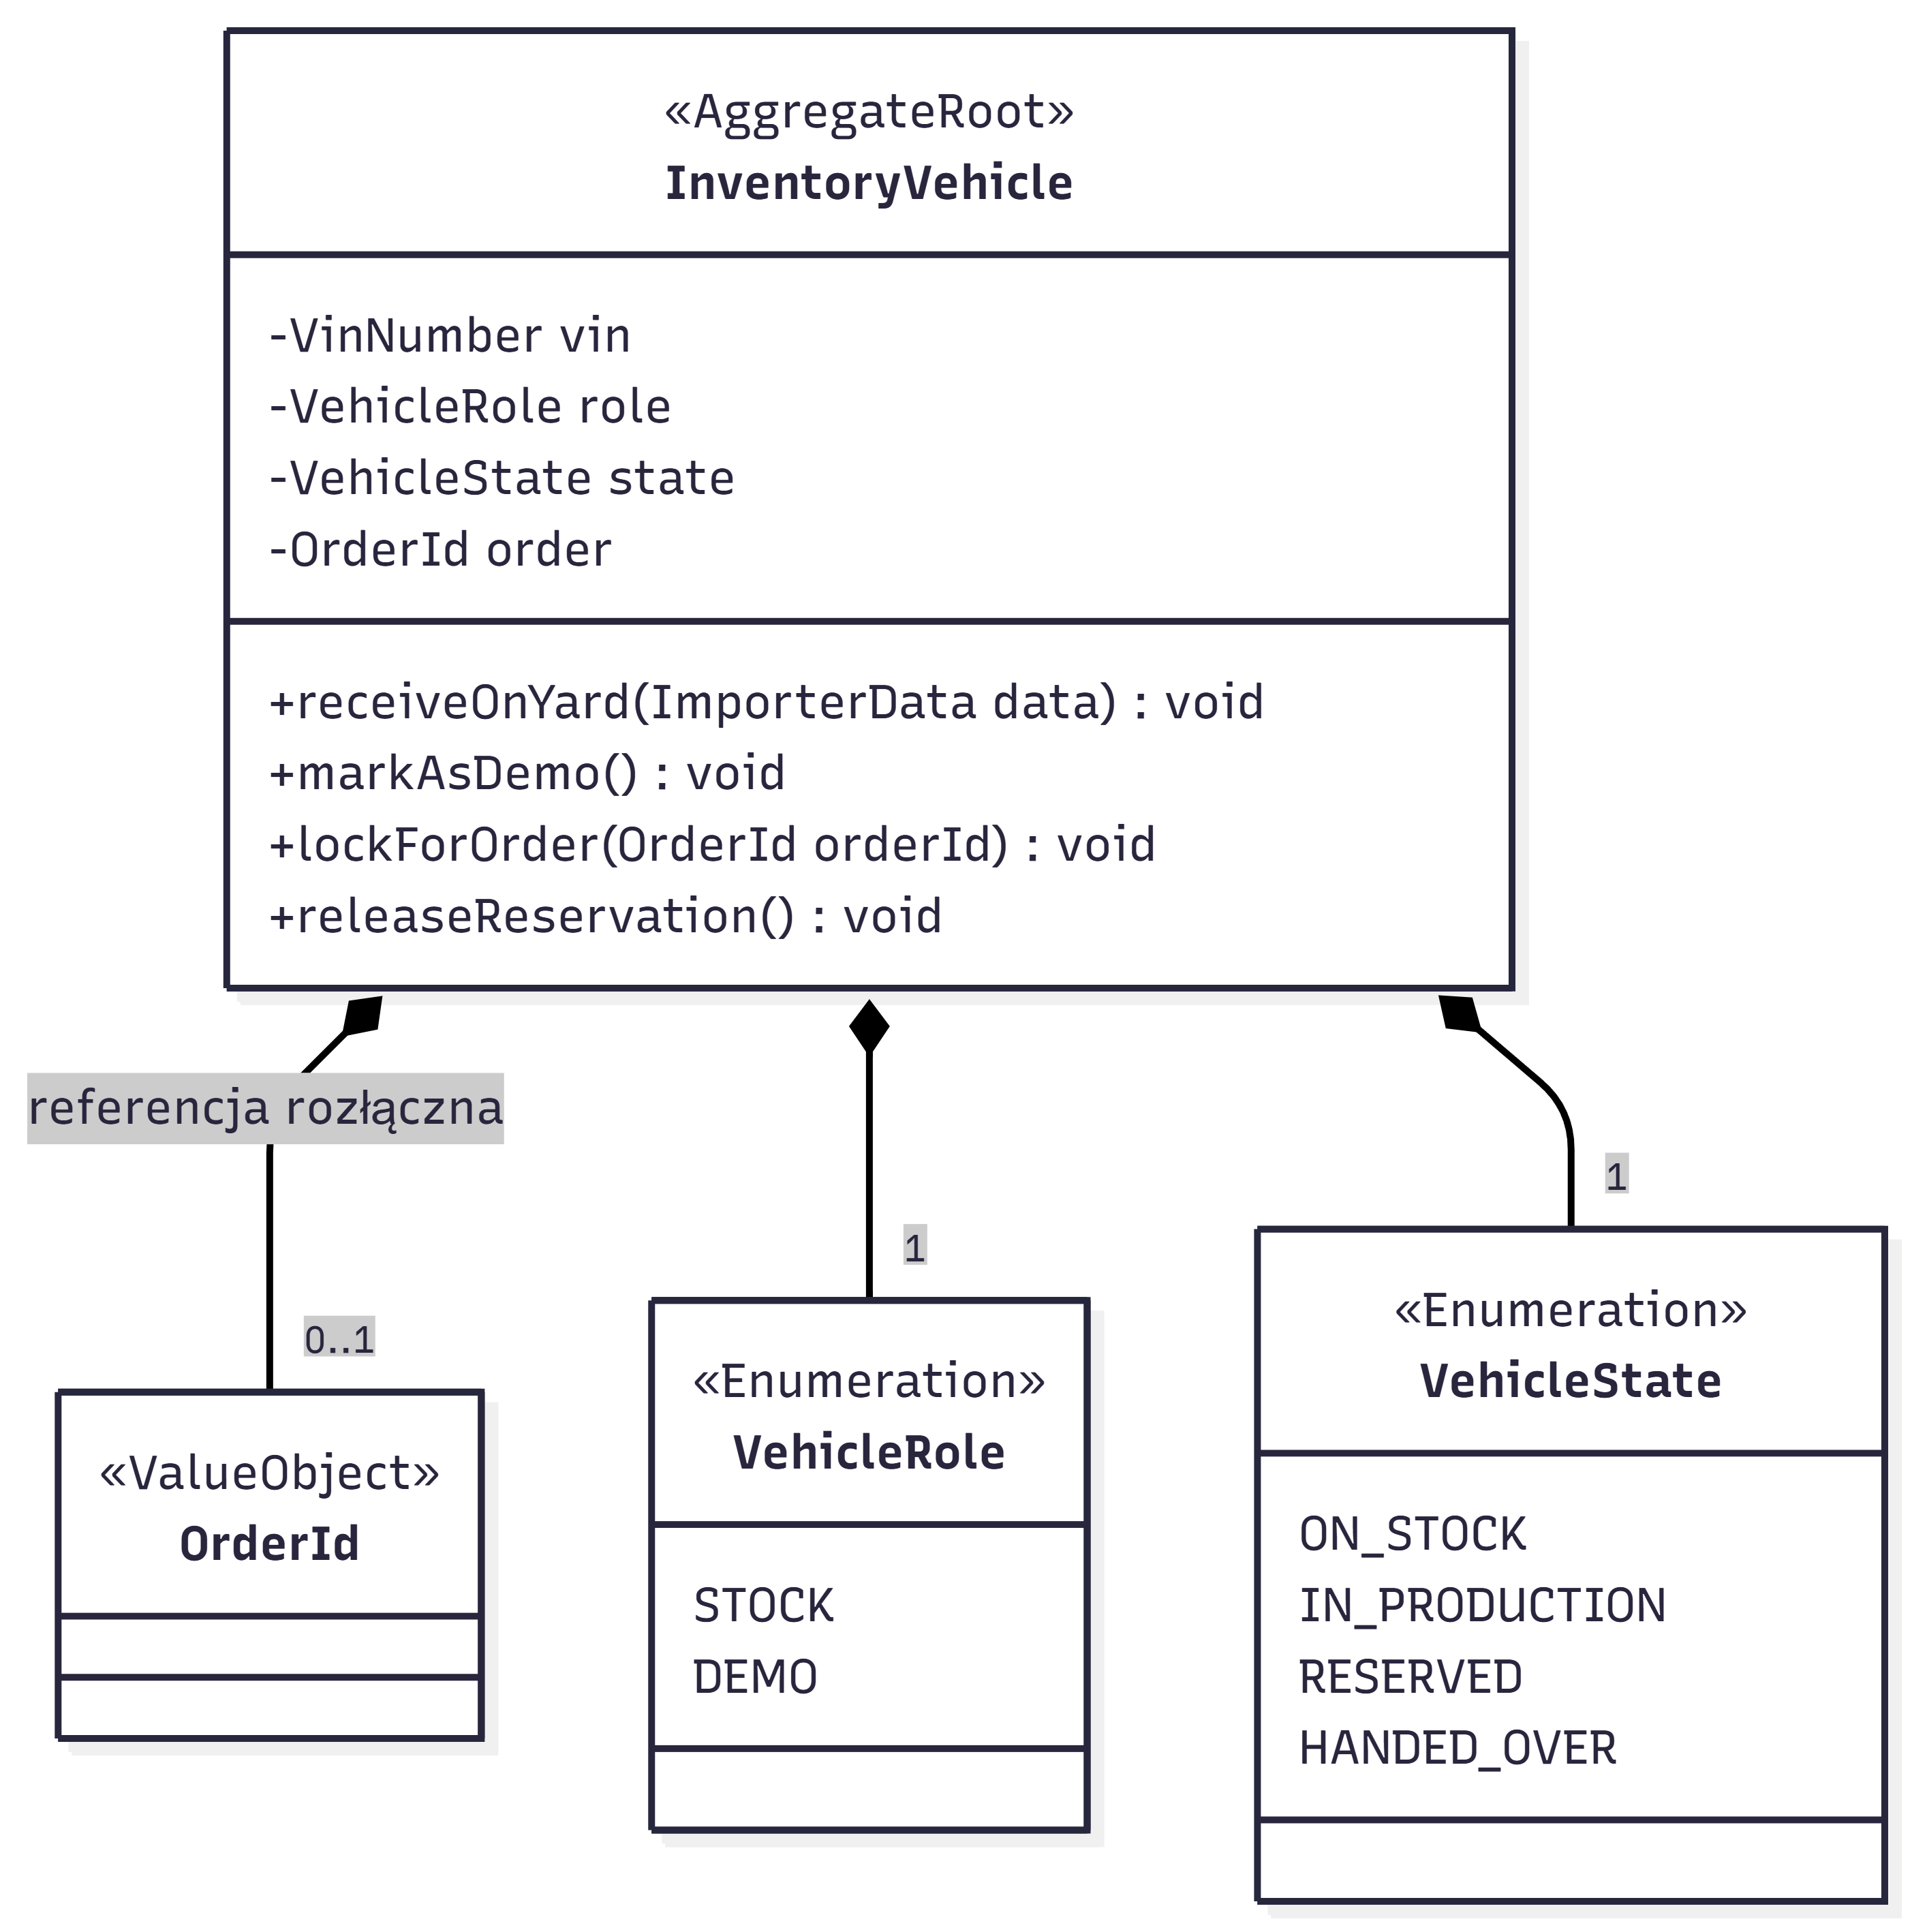
\includegraphics[width=0.5\textwidth]{media/agregaty/kontekst-inwentarza-logistyki/inventory-vehicle.png}
    \caption{Model strukturalny agregatu Fizycznego Egzemplarza Pojazdu}
    \label{fig:agg_vehicle}
\end{figure}

\paragraph{Agregat: Pojazd Magazynowy (InventoryVehicle)}
Stanowi centralny i jedyny korzeń agregatu (Aggregate Root) w Kontekście Inwentarza i Logistyki. Reprezentuje on cykl życia pojazdu w ekosystemie dealera – łącząc fazę wirtualną (zamówienie w produkcji) z fazą fizyczną (obecność na placu magazynowym). Odpowiada za utrzymanie integralności danych logistycznych i zapobieganie konfliktom rezerwacji.

\begin{itemize}
    \item \textbf{Rygorystyczna Maszyna Stanów (State Machine):} Cykl życia pojazdu kontrolowany jest przez wewnętrzną enumerację \texttt{VehicleState}. Agregat kategorycznie chroni przejścia między stanami (\texttt{IN\_PRODUCTION}, \texttt{ON\_STOCK}, \texttt{RESERVED}, \texttt{HANDED\_OVER}). Mutacje stanu odbywają się wyłącznie poprzez wysoce ekspresywne metody biznesowe. Przykładowo, metoda \texttt{receiveOnYard()} transformuje wirtualne auto z fabryki w fizyczny zasób na placu, a metoda \texttt{lockForOrder()} zmienia status na zarezerwowany.
    \item \textbf{Referencja Rozłączna i Ochrona Rezerwacji:} Powiązanie fizycznego auta z umową sprzedażową realizowane jest poprzez opcjonalny obiekt wartości \texttt{OrderId} (krotność 0..1). Agregat implementuje wzorzec twardej blokady (Pessimistic/Optimistic Locking na poziomie domeny) – metoda \texttt{lockForOrder()} hermetyzuje przypisanie zamówienia do numeru VIN, uniemożliwiając tzw. \textit{double-booking} (sprzedaż tego samego auta dwóm klientom). W przypadku zerwania umowy, metoda \texttt{releaseReservation()} czyści referencję, przywracając pojazd do wolnej puli.
    \item \textbf{Polityka Przeznaczenia (\texttt{VehicleRole}):} Aby uniknąć tworzenia nadmiarowych podklas (np. \texttt{DemoVehicle}, \texttt{StockVehicle}), agregat wykorzystuje kompozycję z enumeracją \texttt{VehicleRole}. Dzięki metodzie \texttt{markAsDemo()}, system może w dowolnym momencie wykluczyć pojazd ze standardowej puli sprzedażowej i przeznaczyć go do jazd testowych, zachowując pełną historię jego numeru VIN.
    \item \textbf{Globalna Tożsamość:} Podstawowym identyfikatorem agregatu w późniejszych fazach cyklu życia jest obiekt wartości \texttt{VinNumber}. Gwarantuje on unikalność zasobu i stanowi naturalny klucz integracyjny dla logistyki placowej (np. podczas skanowania zjazdów z lawety w procesie UC-INW-03).
\end{itemize}

\newpage
\subsection{Kontekst Finansowania}
Kontekst Finansowania to poddziedzina generyczna (\textit{Generic Subdomain}), która stanowi most komunikacyjny pomiędzy salonem samochodowym a rynkiem usług finansowych (banki, firmy leasingowe). Głównym wyzwaniem architektonicznym w tym obszarze jest zapewnienie niezawodnej komunikacji i translacji danych przy jednoczesnej ochronie jądra systemu przed zmieniającymi się standardami zewnętrznych interfejsów API.

\subsubsection{Kanwa Kontekstu Finansowania}
\begin{figure}[H]
    \centering
    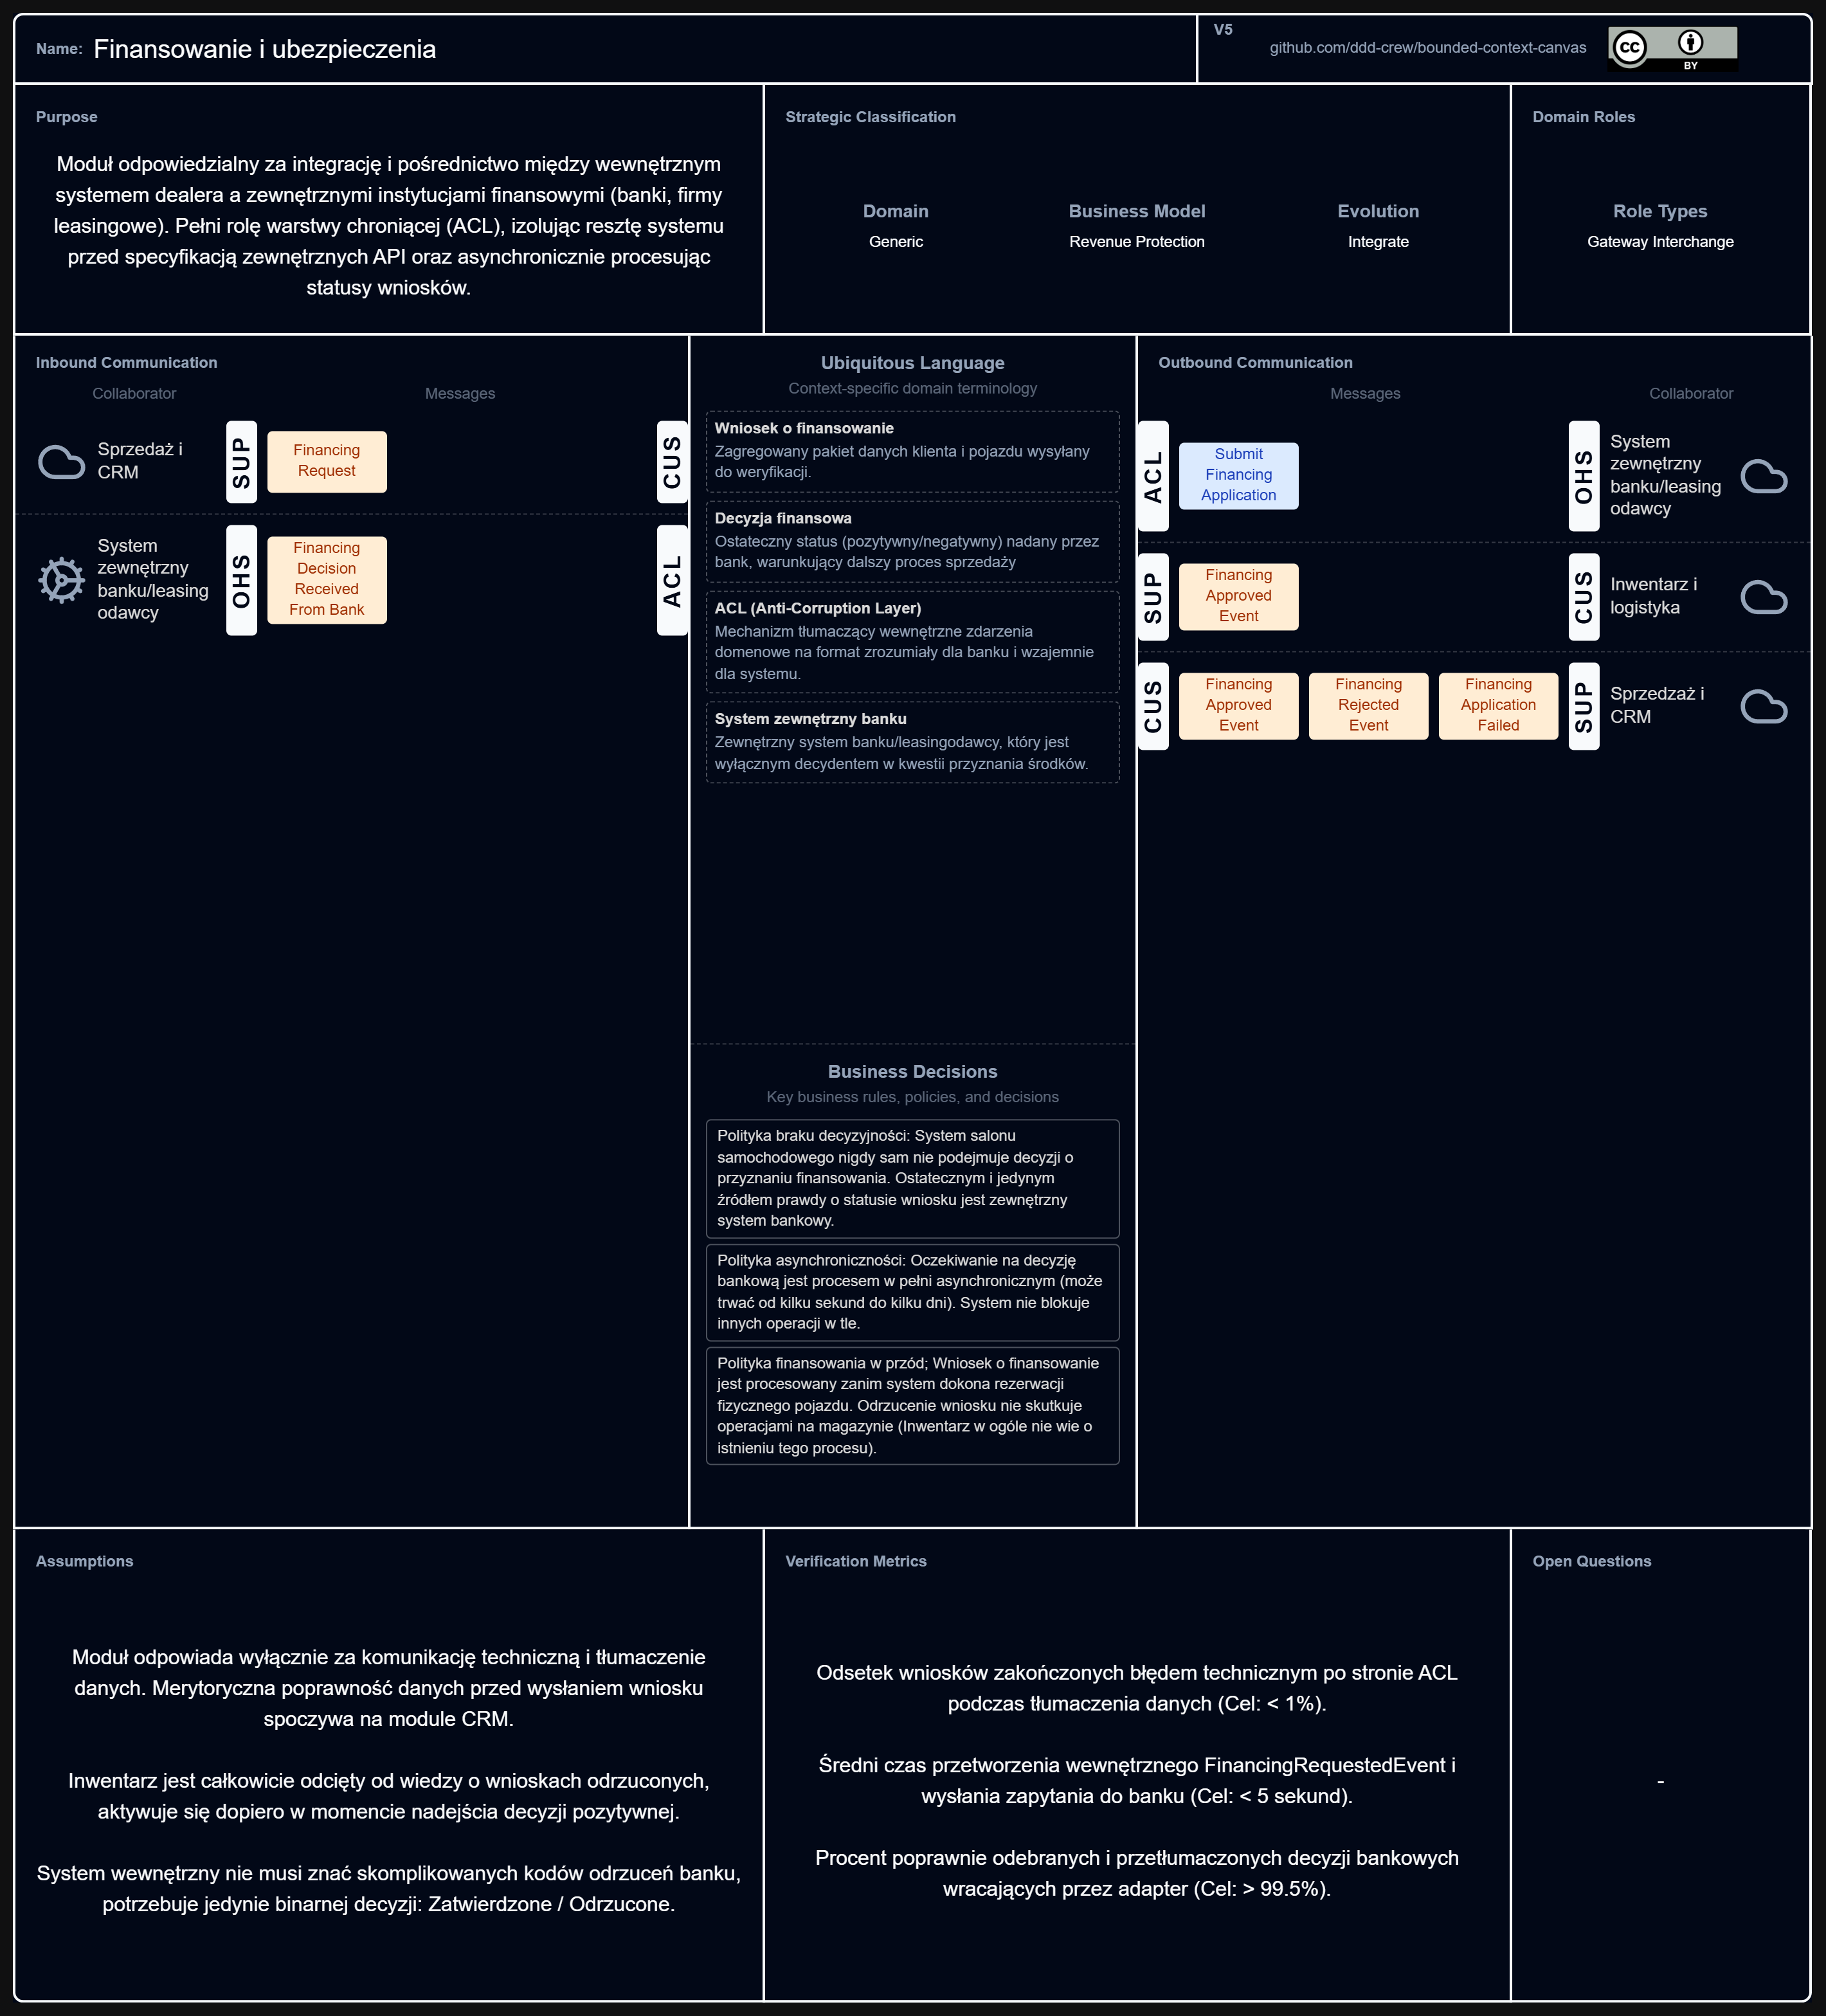
\includegraphics[width=\textwidth]{media/bounded-context-canvas/final/FIU_K6_TOTAL_FINAL.png}
    \caption{Kanwa Kontekstu Kontekstu Finansowania}
    \label{fig:hex_billing}
\end{figure}


\subsubsection{Przypadki użycia Kontekstu Finansowania}
% =====================================================
\textbf{UC-FIN-01: Złożenie wniosku o finansowanie}

\begin{longtable}{|p{4cm}|p{11cm}|}
\hline
\textbf{Element} & \textbf{Opis} \\
\hline

Identyfikator & UC-FIN-01 \\
\hline

Nazwa & Złożenie wniosku o finansowanie \\
\hline

Opis & 
Proces zebrania danych z zamówienia, ich translacji i wysłania zapytania o zdolność kredytową/leasingową klienta do systemu bankowego. \\
\hline

Aktor główny & System (Kontekst Finansowania) \\
\hline

Aktorzy pomocniczy & System zewnętrzny banku \\
\hline

Warunki wstępne & 
Kontekst otrzymał zdarzenie \textit{FinancingRequestedEvent} (Klient w CRM zdecydował się na leasing/kredyt i podał wymagane dane). \\
\hline

Warunki końcowe & 
Wniosek zostaje wysłany do systemu zewnętrznego banku, a system oczekuje na decyzję (status finansowania: Oczekujący). \\
\hline

Scenariusz główny & 
\begin{enumerate}
    \item Kontekst reaguje na zdarzenie \textit{FinancingRequestedEvent}.
    \item System agreguje dane pojazdu (cena, VIN/model) oraz dane klienta (NIP, dochody).
    \item System tłumaczy (poprzez ACL) dane na strukturę wymaganą przez API banku (np. dedykowany JSON/XML).
    \item System wysyła żądanie autoryzacji do systemu zewnętrznego banku.
    \item System oznacza wniosek lokalnie statusem "W trakcie weryfikacji bankowej".
\end{enumerate} \\
\hline

Scenariusze alternatywne & 
\begin{itemize}
    \item [A1] Błąd komunikacji z bankiem: API banku nie odpowiada, system zawiesza proces i ponawia próbę po określonym czasie.
    \item [A2] Odrzucenie walidacji po stronie banku: System banku natychmiast zwraca błąd o braku wymaganych danych (np. błędny NIP). System emituje zdarzenie \textit{FinancingApplicationFailed}, aby handlowiec poprawił wniosek wraz z Klientem.
\end{itemize} \\
\hline
\end{longtable}

\begin{figure}[H]
    \centering
    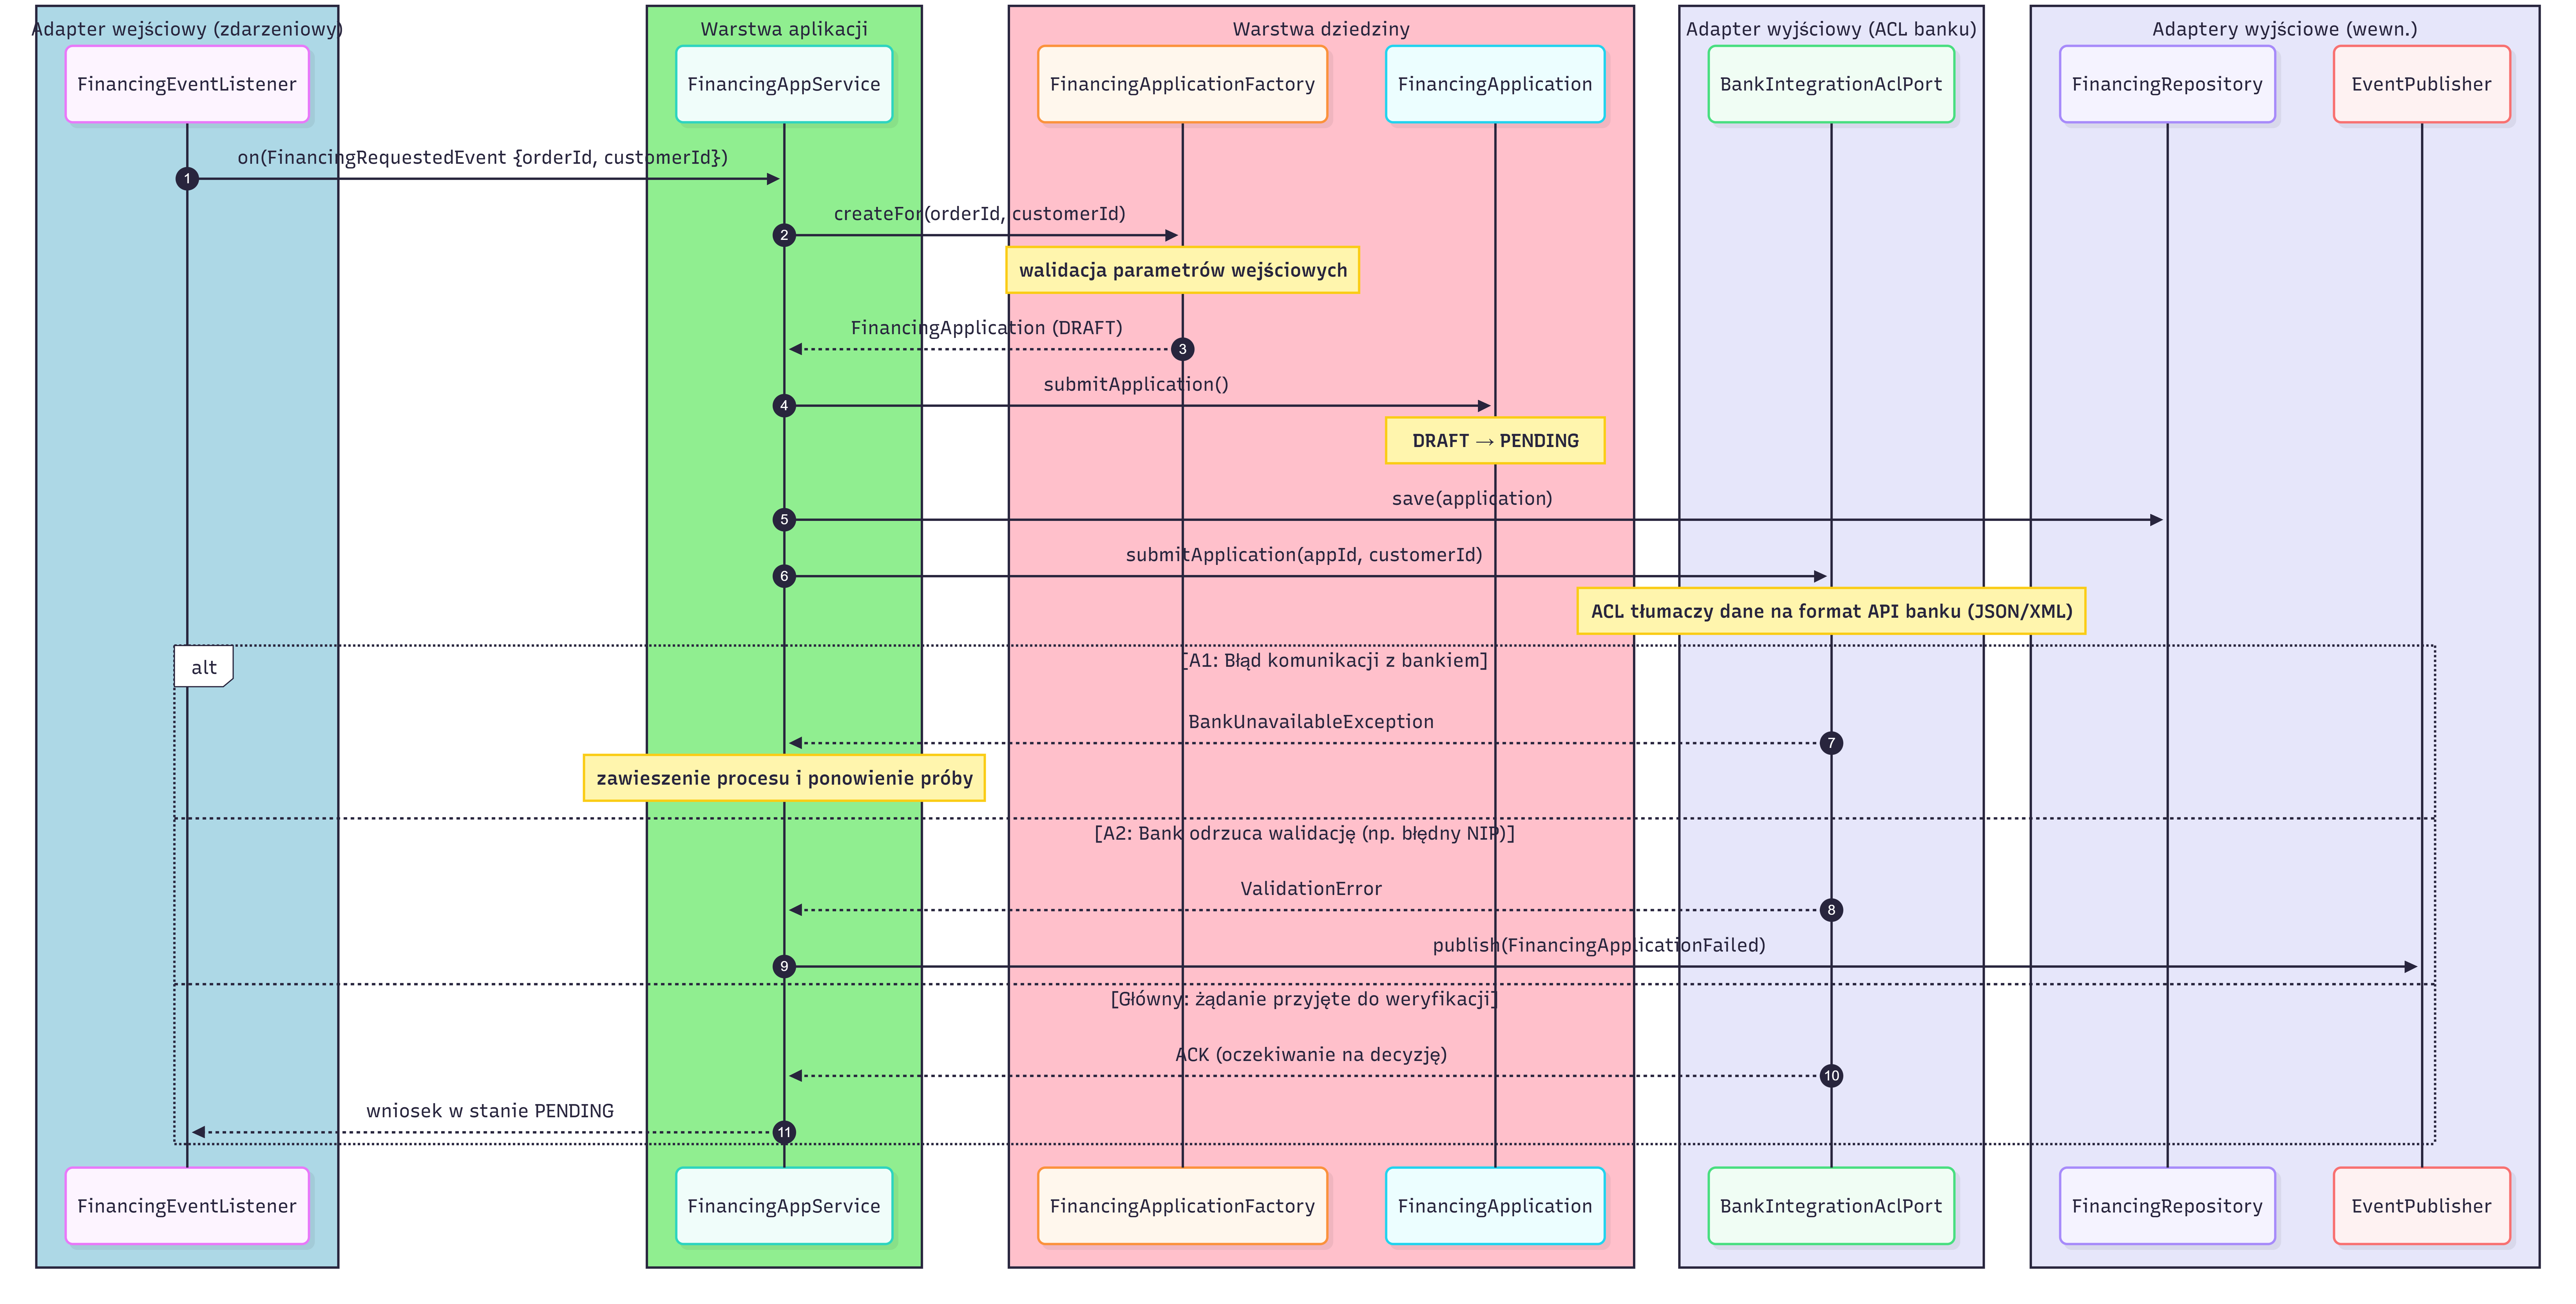
\includegraphics[width=1\textwidth]{media/diagramy_sekwencji/kontekst-finansowania/UC-FIN-01-Sekwencji.png}
    \caption{Diagram sekwencji dla przypadku użycia UC-FIN-01: Złożenie wniosku o finansowanie}
    \label{fig:seq_uc_fin_01}
\end{figure}

% =====================================================
\textbf{UC-FIN-02: Przetworzenie decyzji o finansowaniu}

\begin{longtable}{|p{4cm}|p{11cm}|}
\hline
\textbf{Element} & \textbf{Opis} \\
\hline

Identyfikator & UC-FIN-02 \\
\hline

Nazwa & Przetworzenie decyzji o finansowaniu \\
\hline

Opis & 
Odbiór i procesowanie asynchronicznej decyzji z banku oraz ogłoszenie jej wyniku wewnątrz systemu. \\
\hline

Aktor główny & System (Kontekst Finansowania i Ubezpieczeń) \\
\hline

Aktorzy pomocniczy & Adapter bankowy \\
\hline

Warunki wstępne & 
W systemie istnieje wniosek o finansowanie o statusie "W trakcie weryfikacji bankowej". Kontekst otrzymał zdarzenie z adaptera bankowego \textit{FinancingDecisionReceivedFromBank}. \\
\hline

Warunki końcowe & 
Decyzja zapisana w systemie, wyemitowane odpowiednie zdarzenie końcowe \textit{FinancingApprovedEvent} lub \textit{FinancingRejectedEvent}. \\
\hline

Scenariusz główny & 
\begin{enumerate}
    \item System reaguje na zdarzenie \textit{FinancingDecisionReceivedFromBank}.
    \item System bankowy przekazuje pozytywną decyzję o finansowaniu.
    \item System weryfikuje odpowiedź i aktualizuje status wniosku w lokalnej bazie.
    \item System emituje zdarzenie \textit{FinancingApprovedEvent}.
\end{enumerate} \\
\hline

Scenariusze alternatywne & 
\begin{itemize}
    \item [A1] Decyzja odmowna: W kroku 2 system zewnętrzny banku przekazuje decyzję negatywną. System (po weryfikacji) emituje zdarzenie \textit{FinancingRejectedEvent}.
\end{itemize} \\
\hline
\end{longtable}

\begin{figure}[H]
    \centering
    \includegraphics[width=1\textwidth]{media/diagramy_sekwencji/kontekst-finansowania/UC-FIN-02-Sekwencji.png}
    \caption{Diagram sekwencji dla przypadku użycia UC-FIN-02: Przetworzenie decyzji o finansowaniu}
    \label{fig:seq_uc_fin_02}
\end{figure}

\subsubsection{Architektura Kontekstu Finansowania i Wzorzec ACL}

Kontekst Finansowania został zaprojektowany w oparciu o architekturę heksagonalną. Diagram Architektury przedstawiono na rysunku \ref{fig:hex_finance}.

% MIEJSCE NA DIAGRAM ARCHITEKTURY (Finansowanie Flowchart)
\begin{figure}[H]
    \centering
    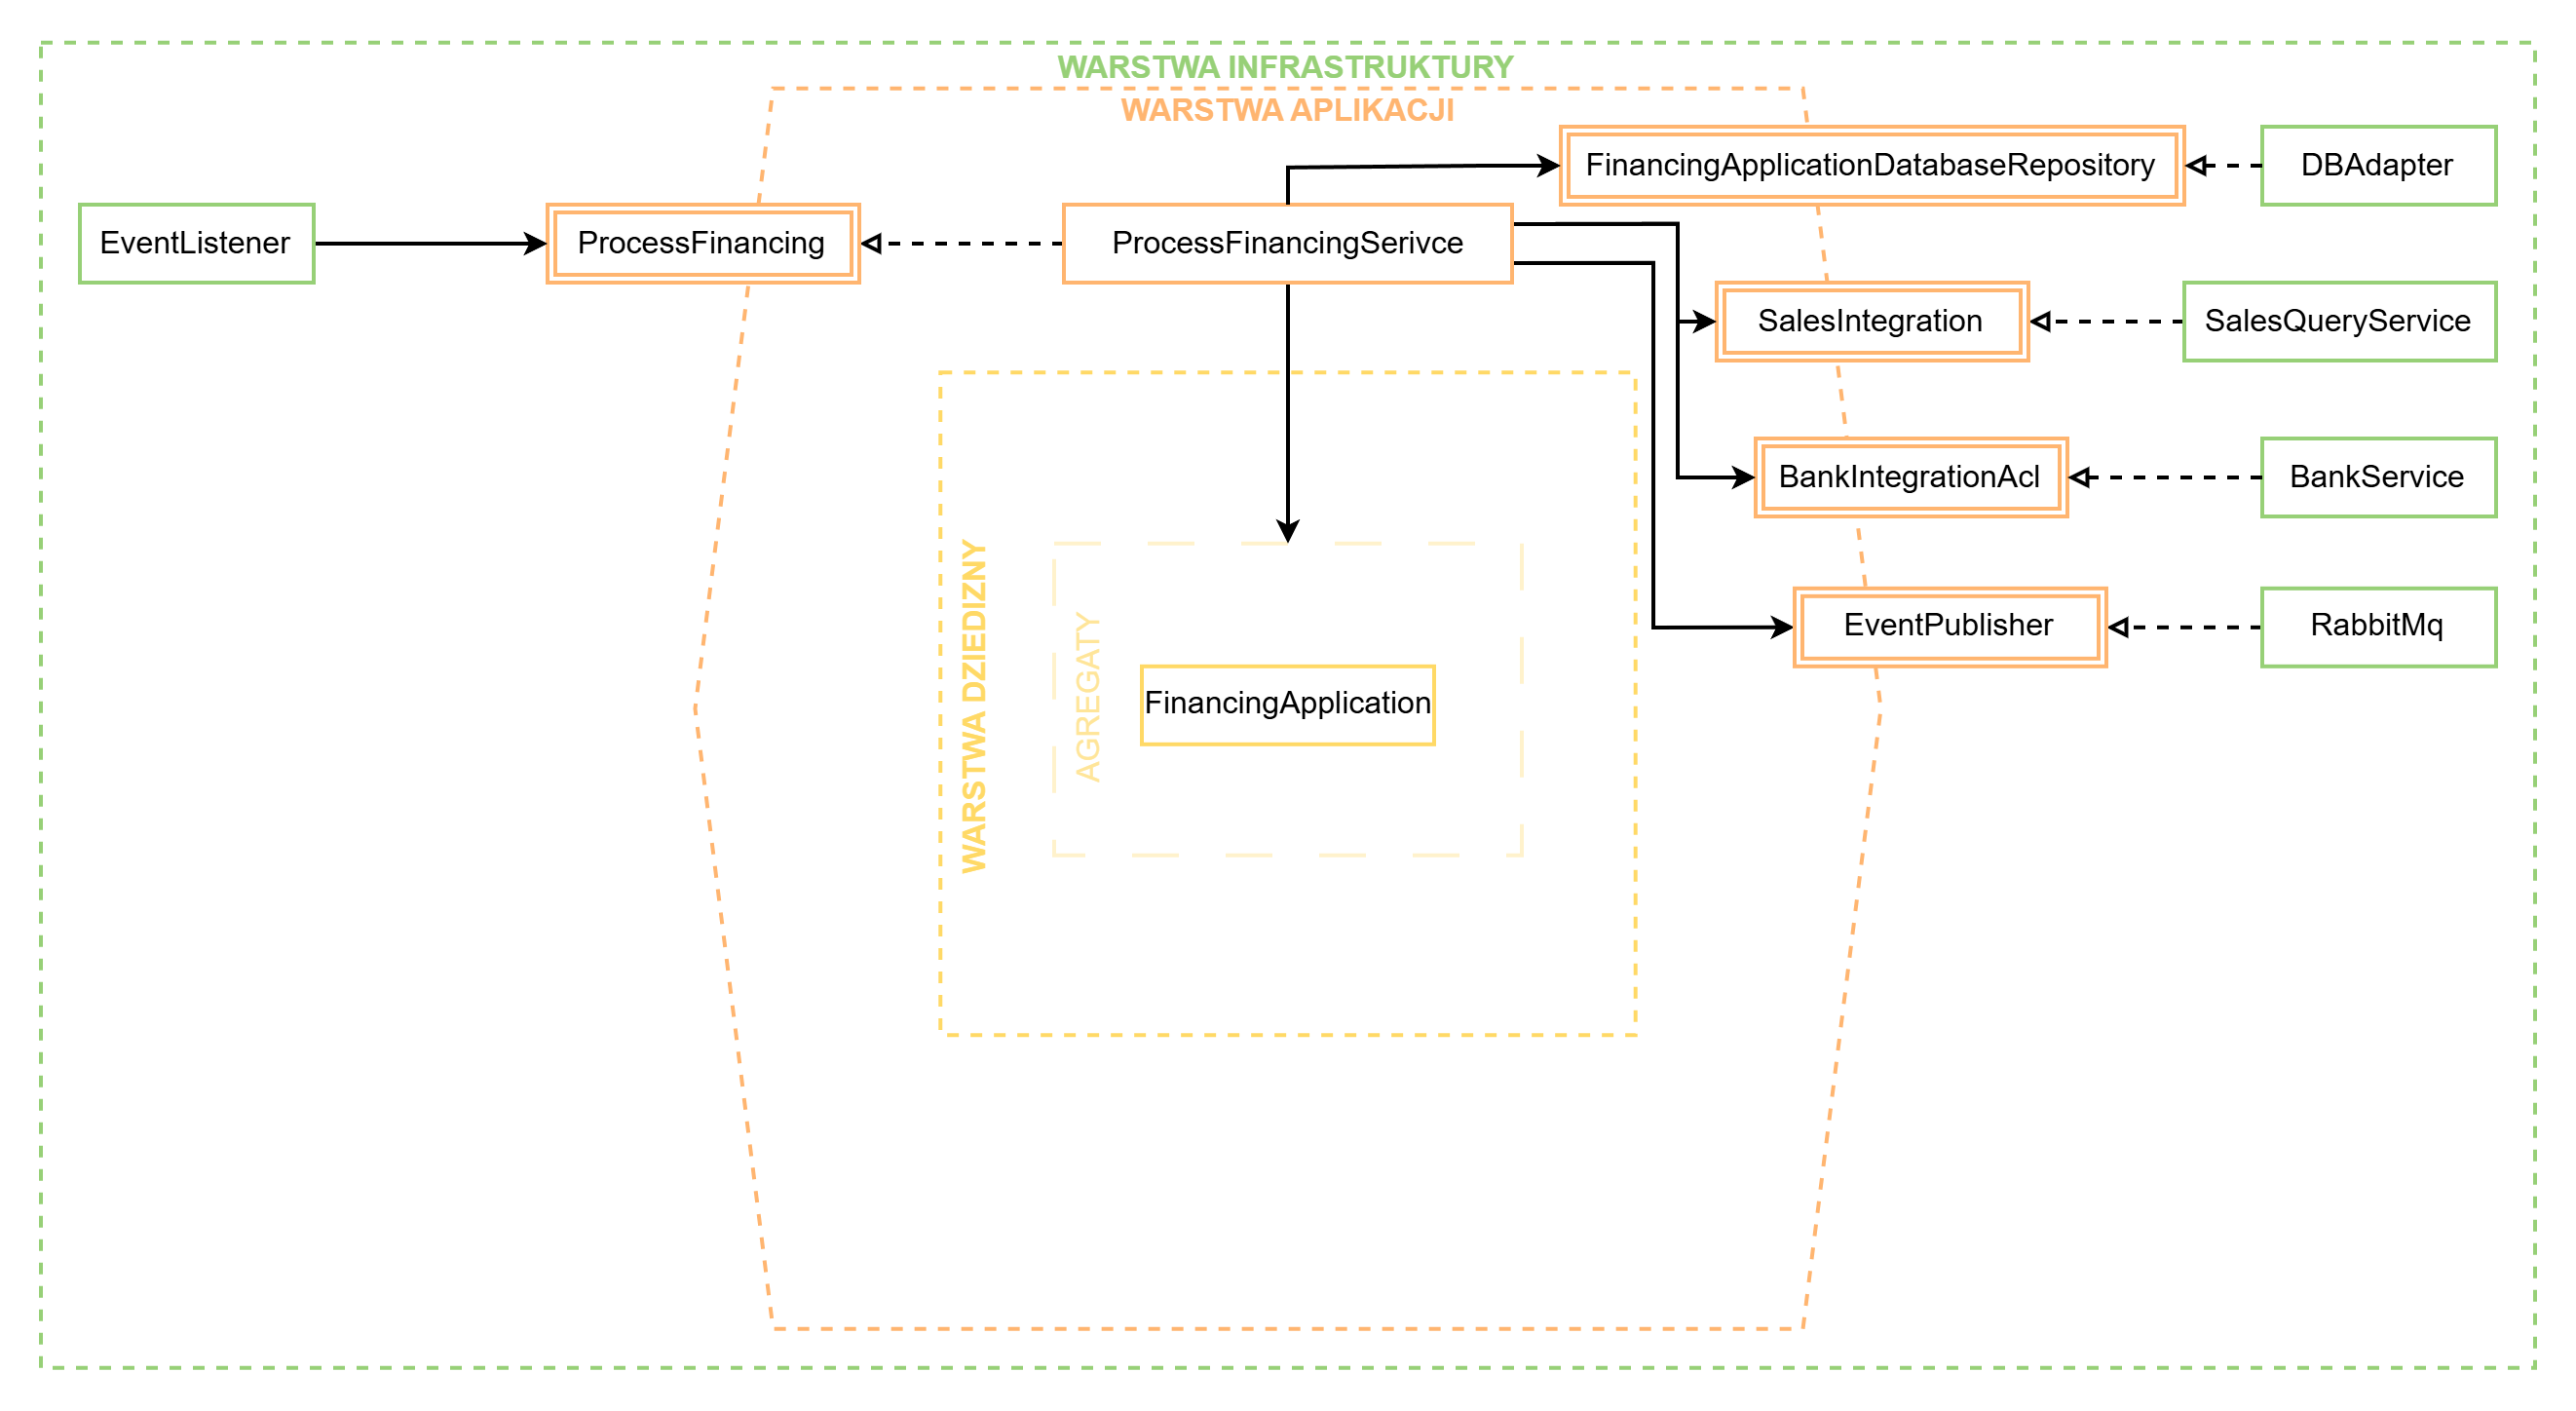
\includegraphics[width=\textwidth]{media/architektura_heksagonalna/FinancingArchitecture.png}
    \caption{Architektura heksagonalna kontekstu finansowania}
    \label{fig:hex_finance}
\end{figure}

Poniżej przedstawiono szczegółowy opis interakcji pomiędzy warstwami, z podziałem na strony wejściową i wyjściową.

\paragraph{Strona Wejściowa: Porty i Adaptery} 
Ta strona heksagonu definiuje, w jaki sposób świat zewnętrzny komunikuje się z Kontekstem Finansowania w celu wyzwolenia procesów oceny zdolności i akceptacji wniosków. Interfejsy wejściowe zestawiono z ich technicznymi implementacjami.

Zgodnie z diagramem Kontekst Finansowania udostępnia \textbf{jeden} port wejściowy obejmujący oba przypadki użycia (złożenie wniosku i przetworzenie decyzji banku), zasilany asynchronicznie zdarzeniami.

\begin{itemize}
    \item \textbf{Obsługa Wniosku o Finansowanie (Asynchroniczne)}
    \begin{itemize}
        \item \textbf{Port:} \texttt{ProcessFinancing}. Jedyny port wejściowy, obejmujący złożenie wniosku (\texttt{requestFinancing}, UC-FIN-01) oraz przetworzenie asynchronicznej decyzji banku (\texttt{processBankDecision}, UC-FIN-02). Realizowany przez usługę aplikacyjną \texttt{ProcessFinancingService}. Salon nie podejmuje decyzji kredytowej — bank jest jedynym decydentem, a port jedynie odzwierciedla nadany przez niego status.
        \item \textbf{Adapter:} \texttt{FinancingEventListener} (Messaging Adapter). Nasłuchuje magistrali zdarzeń: przechwytuje \texttt{FinancingRequested} (z Kontekstu Sprzedaży) i wyzwala \texttt{requestFinancing}, oraz \texttt{FinancingDecisionReceivedFromBank} (z adaptera bankowego) i wyzwala \texttt{processBankDecision}. Komunikaty zewnętrzne reprezentowane są jako lokalne rekordy ACL.
    \end{itemize}
\end{itemize}

\paragraph{Strona Wyjściowa: Porty i Adaptery} 
Ta strona heksagonu definiuje mechanizmy integracji warstwy aplikacji z bazą danych, zewnętrznymi instytucjami weryfikacyjnymi oraz systemem komunikacji asynchronicznej.

\begin{itemize}
    \item \textbf{Utrwalanie Stanu (Persystencja)}
    \begin{itemize}
        \item \textbf{Port:} \texttt{FinancingApplicationDatabaseRepository}. Umożliwia usłudze aplikacyjnej zapis i odczyt agregatu \texttt{FinancingApplication} (indeks po \texttt{OrderId}).
        \item \textbf{Adapter:} \texttt{InMemoryFinancingRepository} (węzeł \texttt{DBAdapter}). W bieżącej implementacji atrapa w pamięci; docelowo adapter bazodanowy (ORM/Hibernate) bez zmiany kontraktu portu.
    \end{itemize}

    \item \textbf{Integracja z Bankiem (Anti-Corruption Layer)}
    \begin{itemize}
        \item \textbf{Port:} \texttt{BankIntegrationAcl}. Dwukierunkowy port wyjściowy do systemu banku — wysyłka wniosku (\texttt{submitFinancingApplication}); bank jest jedynym decydentem, a decyzja wraca później osobnym zdarzeniem.
        \item \textbf{Adapter:} \texttt{BankIntegrationMockAdapter}. Atrapa symulująca asynchroniczne złożenie wniosku; docelowo adapter HTTP do zewnętrznych dostawców usług finansowych, tłumaczący ich API na model domeny (ACL).
    \end{itemize}

    \item \textbf{Integracja ze Sprzedażą i CRM (Anti-Corruption Layer)}
    \begin{itemize}
        \item \textbf{Port:} \texttt{SalesIntegration}. Query Port dociągający dane nabywcy (\texttt{buyerDetails}) oraz cenę końcową oferty (\texttt{offerFinalPrice}) potrzebne do wniosku (UC-FIN-01).
        \item \textbf{Adapter:} \texttt{SalesCrmIntegrationAdapter}. Zależy wyłącznie od fasady Sprzedaży (\texttt{SalesQueryFacade}) i tłumaczy migawki na lokalny model Finansowania (\texttt{BuyerDetails}, \texttt{Money}).
    \end{itemize}

    \item \textbf{Publikacja Zdarzeń}
    \begin{itemize}
        \item \textbf{Port:} \texttt{EventPublisher} (port Wspólnego Jądra). Umożliwia publikację zdarzeń wynikowych na magistralę.
        \item \textbf{Adapter:} \texttt{RabbitMqEventPublisherAdapter} (Wspólne Jądro). Serializuje zdarzenia dziedzinowe o statusie wniosku (np. \texttt{FinancingApprovedEvent}, \texttt{FinancingRejectedEvent}, \texttt{FinancingApplicationFailedEvent}) i wysyła je na magistralę, umożliwiając modułowi Sprzedaży asynchroniczną kontynuację obsługi klienta.
    \end{itemize}
\end{itemize}

\paragraph{Usługi Aplikacji}
Dla kontekstu Finansowania przewidziano jeden centralny komponent orkiestrujący:
\begin{itemize}
    \item \textbf{ProcessFinancingService} – zarządza pełnym cyklem życia wniosku o finansowanie. W ramach UC-FIN-01 dociąga dane nabywcy i kwotę z Kontekstu Sprzedaży (\texttt{SalesIntegration}), tworzy nowy agregat \texttt{FinancingApplication} przez fabrykę (\texttt{createDraft}), wysyła wniosek do banku (\texttt{BankIntegrationAcl}) i utrwala status PENDING. W ramach UC-FIN-02 pobiera wniosek po \texttt{OrderId}, wymusza na nim mutację stanu zgodnie z decyzją banku (\texttt{approve}/\texttt{reject}) i emituje zdarzenia kończące proces.
\end{itemize}

\subsubsection{Agregaty Kontekstu Finansowania}

% MIEJSCE NA DIAGRAM KLAS: FinancingApplication
\begin{figure}[H]
    \centering
    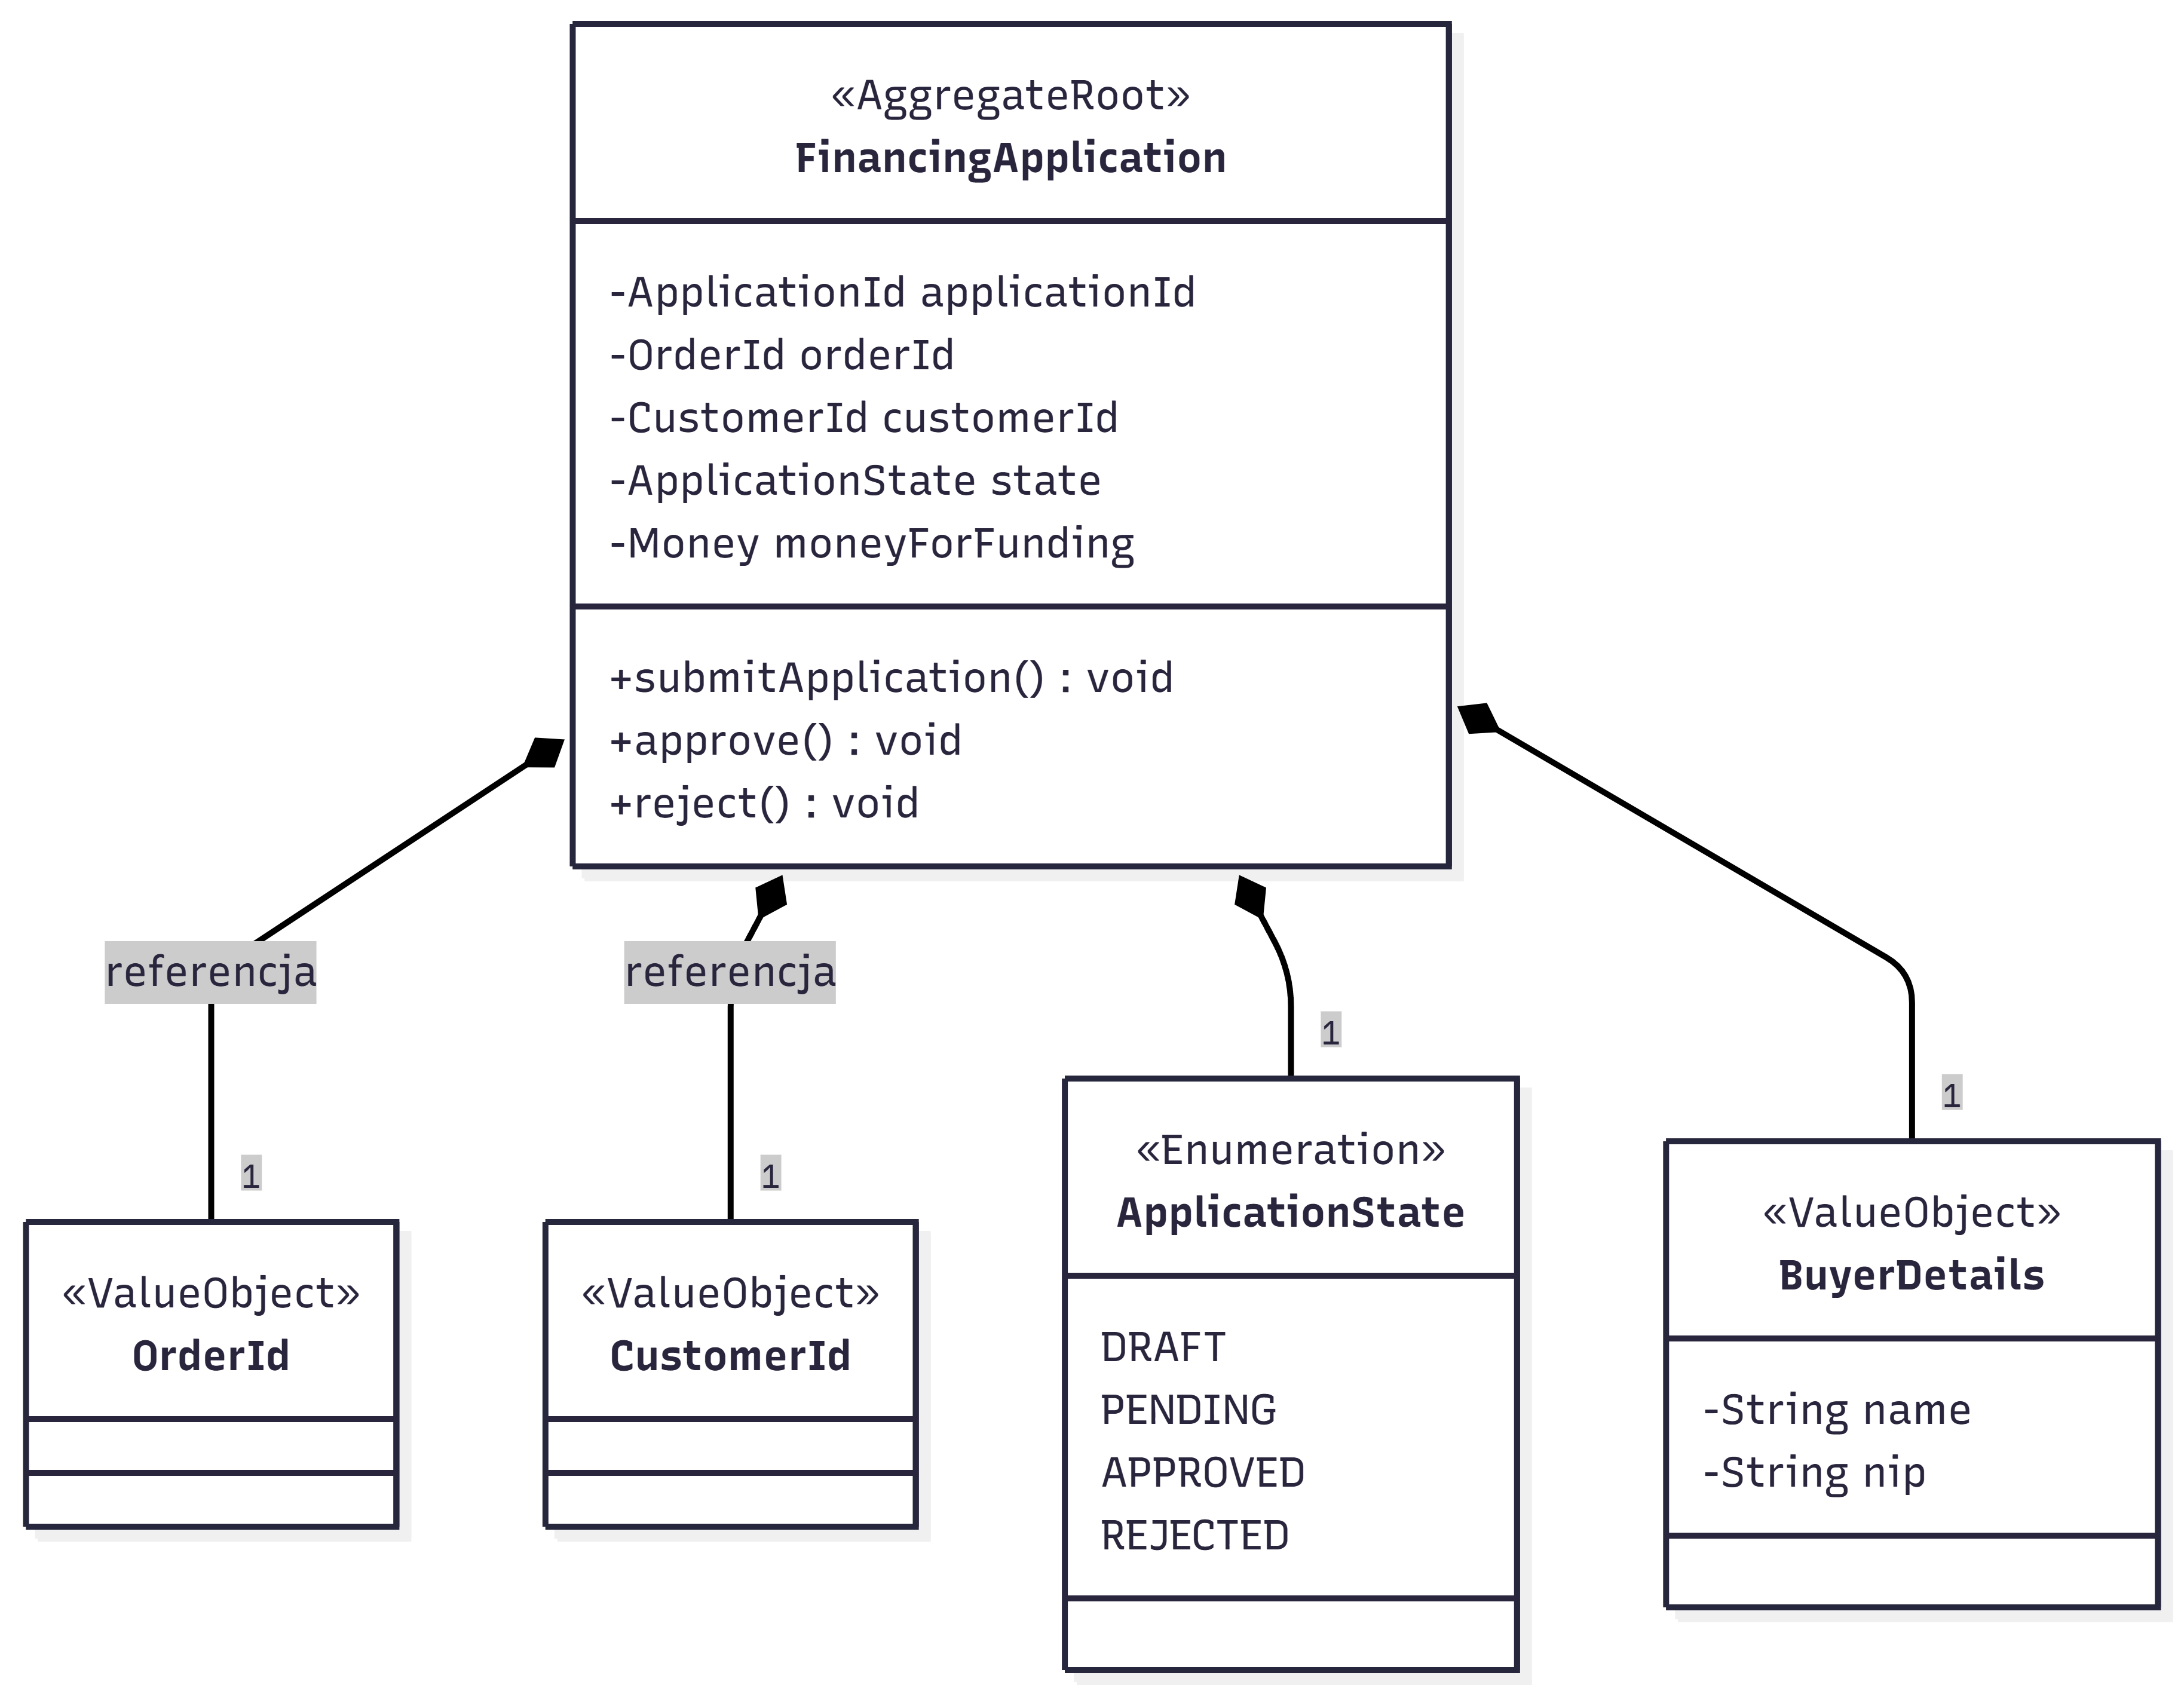
\includegraphics[width=0.5\textwidth]{media/agregaty/kontekst-finansowania/financing-application.png}
    \caption{Model strukturalny agregatu Wniosku Finansowego}
    \label{fig:agg_financing}
\end{figure}

Z uwagi na generyczny i integracyjny charakter tej poddziedziny, zrezygnowano ze skomplikowanych agregatów obliczeniowych na rzecz hermetycznych maszyn stanów.

\paragraph{Agregat: Wniosek Finansowy (FinancingApplication)}
Odpowiada za reprezentację procesu wnioskowania o leasing lub kredyt, powiązanego z danym Zamówieniem. Agregat został maksymalnie zdenormalizowany - nie przechowuje szczegółowych danych finansowych czy analitycznych, skupiając się wyłącznie na bezpiecznym śledzeniu cyklu życia procesu integracyjnego.
\begin{itemize}
    \item \textbf{Maszyna Stanów:} Agregat operuje na ściśle zdefiniowanych stanach (np. \texttt{DRAFT}, \texttt{PENDING}, \texttt{APPROVED}). Zmiana stanu wymuszana jest poprzez hermetyczne metody (\linebreak \texttt{submitApplication}, \texttt{approve}, \texttt{reject}).
    \item \textbf{Ochrona Niezmienników:} Wysłanie wniosku do banku zmienia jego stan na \texttt{PENDING}. Agregat kategorycznie zabrania wywołania metody \texttt{approve()} z jakiegokolwiek innego stanu. Jeśli zewnętrzne API banku w wyniku błędu prześle podwójny webhook z potwierdzeniem finansowania, agregat odrzuci drugą próbę, chroniąc system przed wyemitowaniem zduplikowanych zdarzeń dziedzinowych i podwójnym finansowaniem zamówienia.
    \item \textbf{Sterowanie Przepływem Systemu:} Dopiero pomyślne zatwierdzenie wniosku i zmiana stanu na \texttt{APPROVED} powoduje wewnątrz agregatu wygenerowanie krytycznego zdarzenia \linebreak \texttt{FinancingApprovedEvent}, na które nasłuchuje m.in. Kontekst Rozliczeń, w celu weryfikacji ostatecznego salda kontraktu.
\end{itemize}

\newpage
\subsection{Kontekst Fakturowania i Rozliczeń}
Kontekst Fakturowania i Rozliczeń stanowi wyodrębnioną poddziedzinę systemu, której głównym celem biznesowym jest obsługa wpłat, generowanie prawnie wiążących dokumentów księgowych oraz wyliczanie ostatecznych sald kontraktów. 

\subsubsection{Kanwa Kontekstu Fakturowania i Rozliczeń}

\begin{figure}[H]
    \centering
    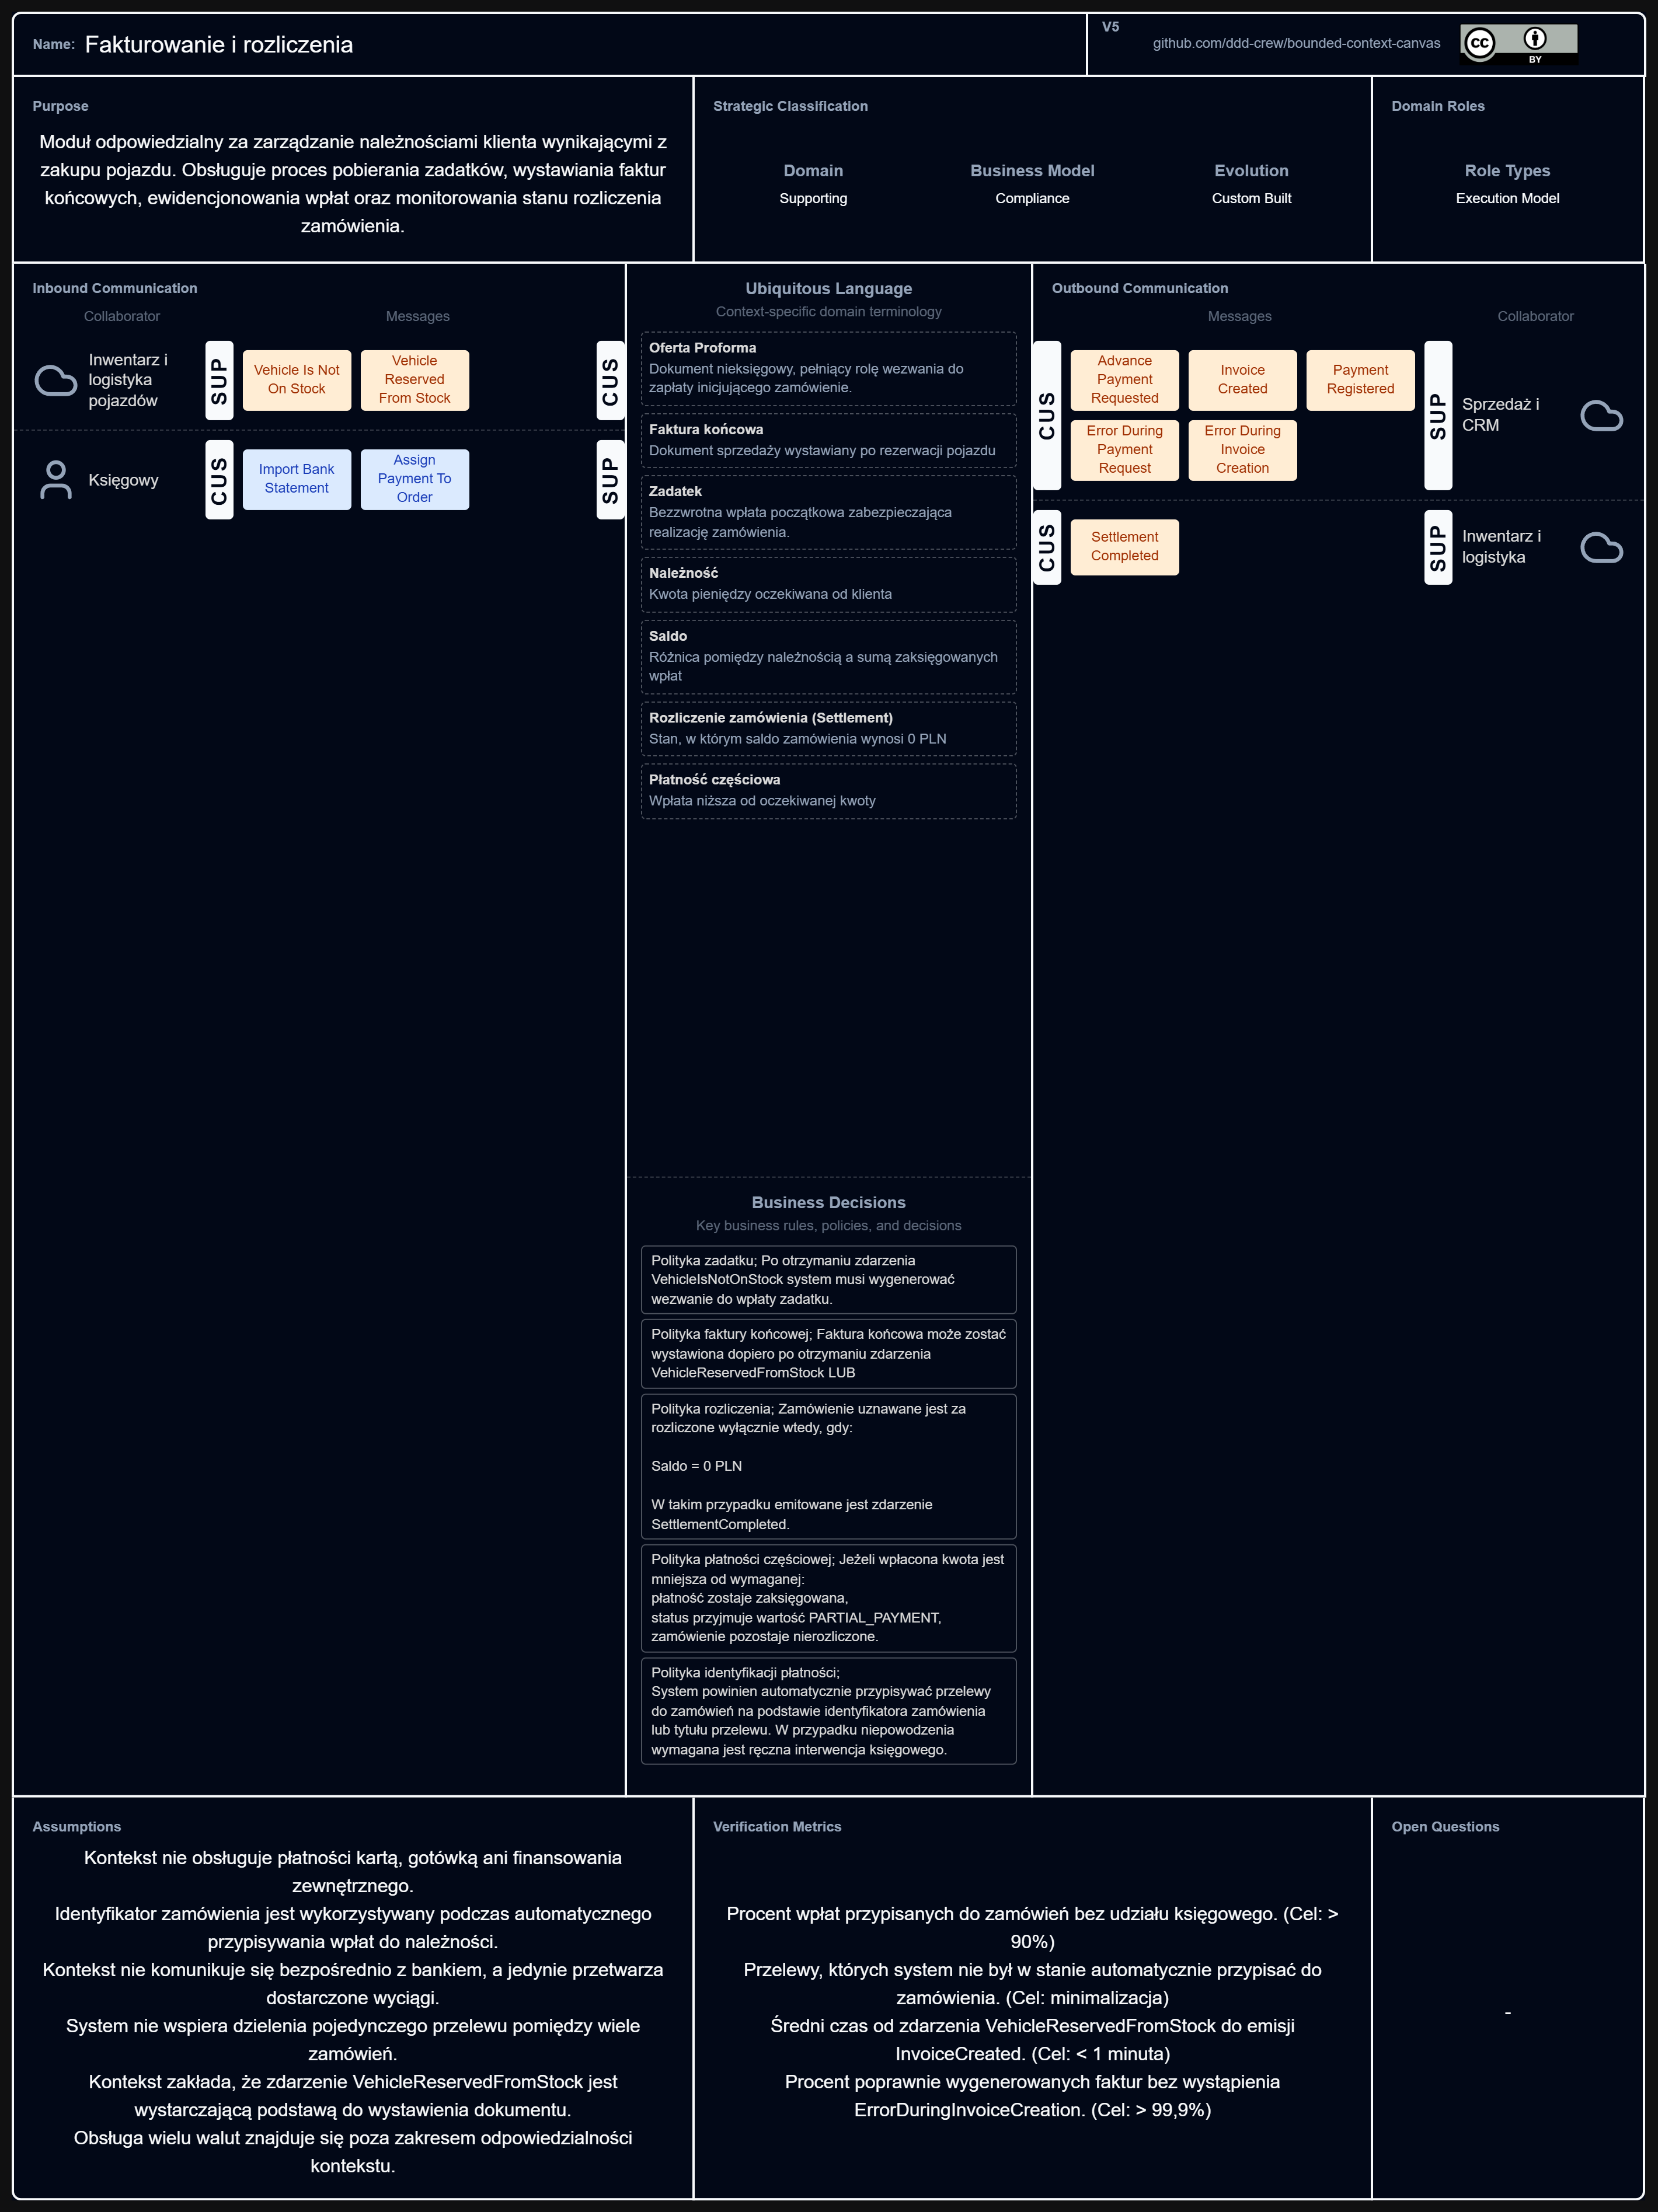
\includegraphics[width=0.9\textwidth]{media/bounded-context-canvas/final/FIR_K7_TOTAL_FINAL.png}
    \caption{Kanwa Kontekstu Fakturowania i Rozliczeń}
    \label{fig:hex_billing}
\end{figure}


\subsubsection{Przypadki użycia Kontekstu Fakturowania i Rozliczeń}

% =====================================================
\textbf{UC-FIR-01: Wysłanie prośby o zadatek}

\begin{longtable}{|p{4cm}|p{11cm}|}
\hline
\textbf{Element} & \textbf{Opis} \\
\hline

Identyfikator & UC-FIR-01 \\
\hline

Nazwa & Wysłanie prośby o zadatek \\
\hline

Opis & 
Przygotowanie danych do przelewu i powiadomienie klienta o konieczności wpłaty zadatku w przypadku braku pojazdu na placu. \\
\hline

Aktor główny & System (Kontekst Fakturowania) \\
\hline

Aktorzy pomocniczy & Klient \\
\hline

Warunki wstępne & 
Kontekst otrzymał zdarzenie \textit{VehicleIsNotOnStock}. \\
\hline

Warunki końcowe & 
Klient został poinformowany o wymaganej wpłacie, emitowane zdarzenie \textit{AdvancePaymentRequested}. \\
\hline

Scenariusz główny & 
\begin{enumerate}
    \item Kontekst fakturowania reaguje na zdarzenie \textit{VehicleIsNotOnStock}.
    \item System generuje numer rachunku bankowego oraz kwotę zadatku dla zamówienia.
    \item System wysyła do klienta informację (np. e-mail) z danymi do przelewu.
    \item Kontekst emituje zdarzenie \textit{AdvancePaymentRequested}.
\end{enumerate} \\
\hline

Scenariusze alternatywne & 
\begin{itemize}
    \item [A1] Błąd danych: Brak wymaganych informacji do wygenerowania prośby, system emituje \textit{ErrorDuringPaymentRequest}.
\end{itemize} \\
\hline
\end{longtable}

\begin{figure}[H]
    \centering
    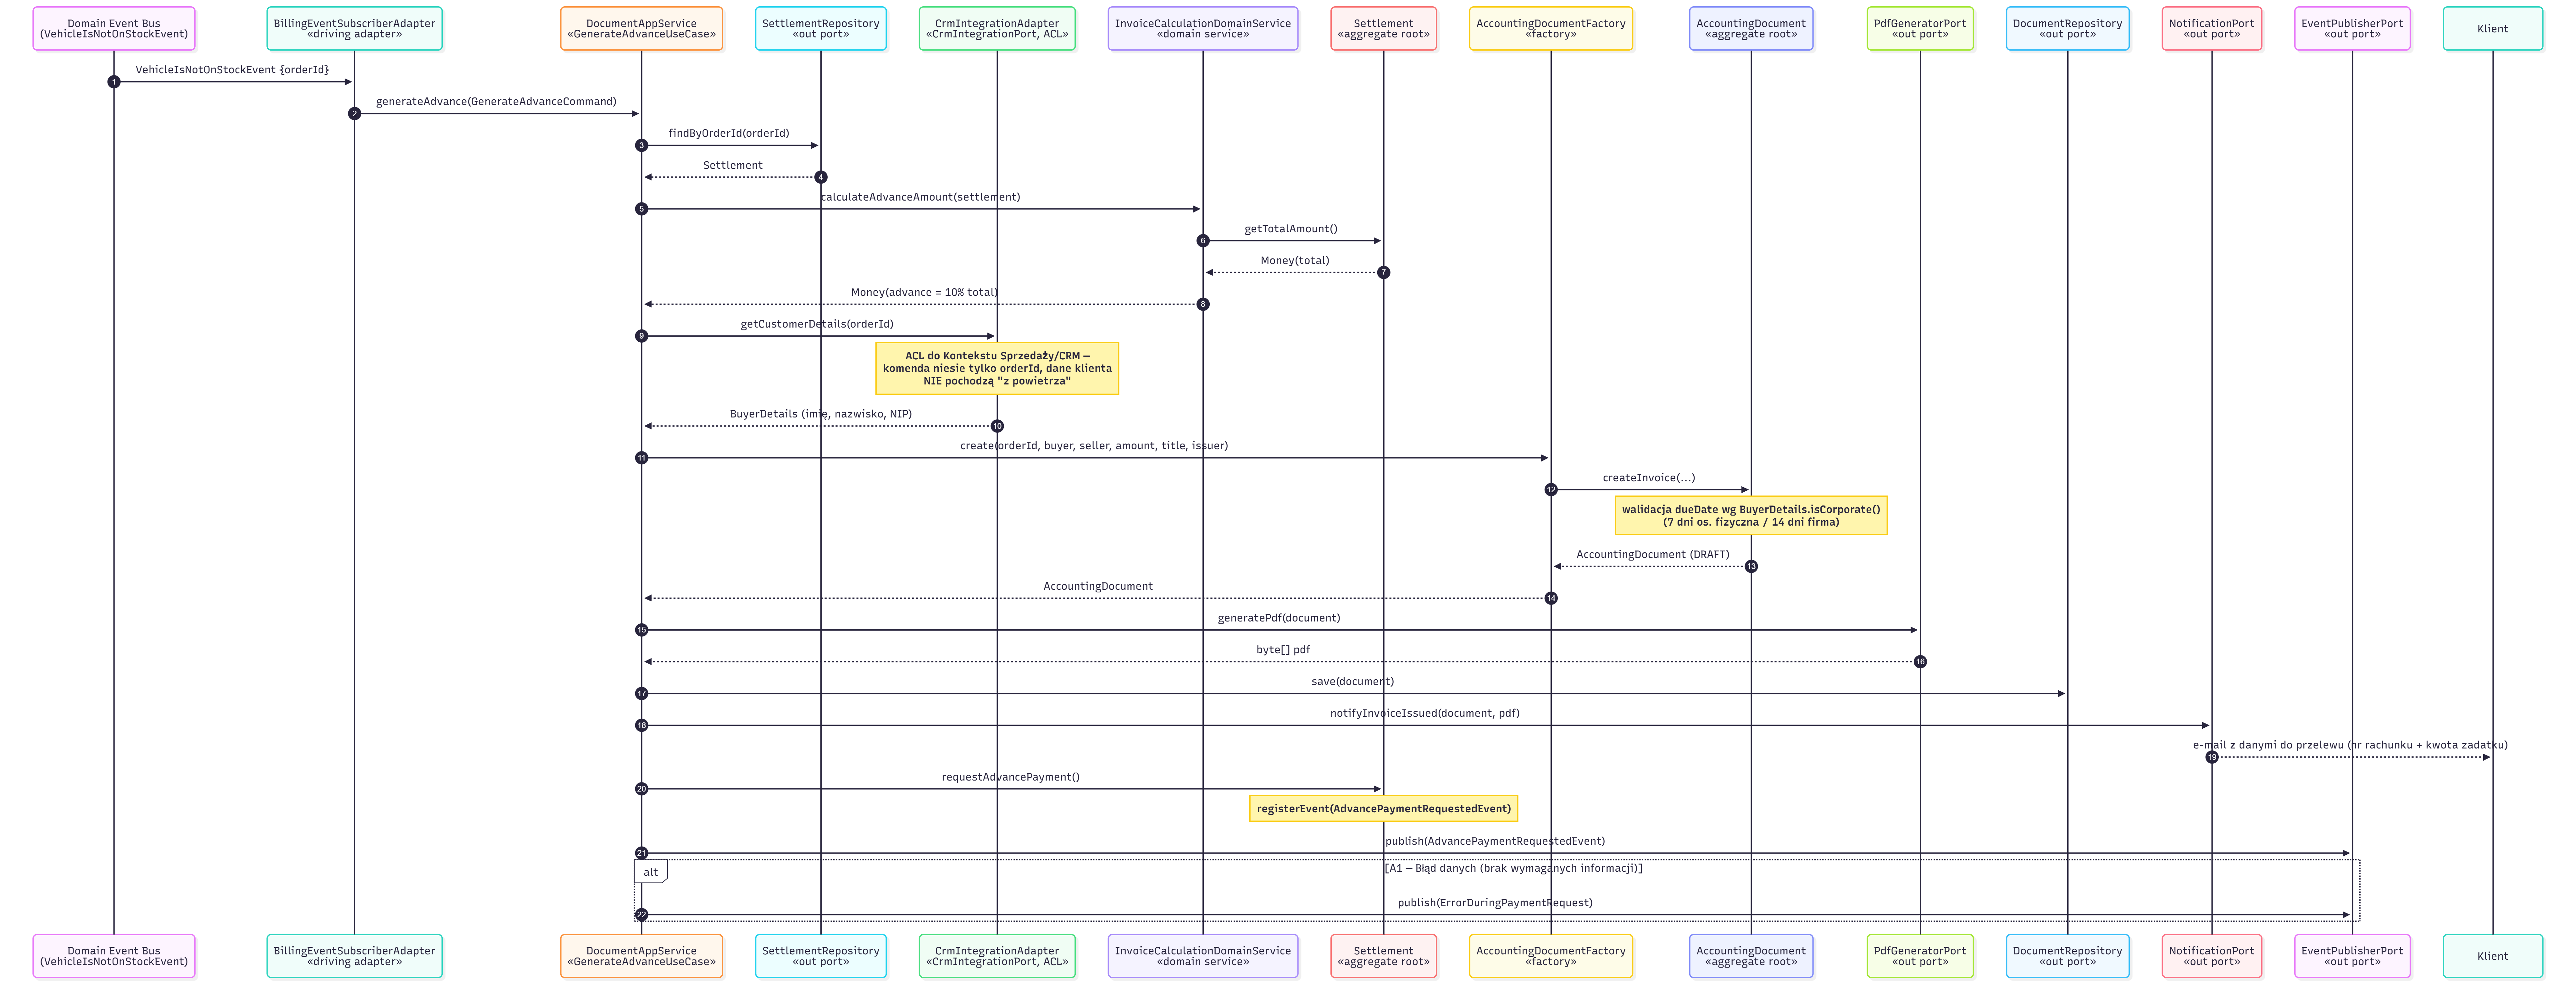
\includegraphics[width=1\textwidth]{media/diagramy_sekwencji/kontekst-faktur-rozliczenia/UC-FIR-01-Sekwencji.png}
    \caption{Diagram sekwencji dla przypadku użycia UC-FIR-01: Wysłanie prośby o zadatek}
    \label{fig:seq_uc_fir_01}
\end{figure}

% =====================================================
\textbf{UC-FIR-02: Stworzenie faktury końcowej}

\begin{longtable}{|p{4cm}|p{11cm}|}
\hline
\textbf{Element} & \textbf{Opis} \\
\hline

Identyfikator & UC-FIR-02 \\
\hline

Nazwa & Stworzenie faktury końcowej \\
\hline

Opis & 
Automatyczne wystawienie faktury końcowej po potwierdzeniu rezerwacji pojazdu z placu. \\
\hline

Aktor główny & System (Kontekst Fakturowania) \\
\hline

Aktorzy pomocniczy & - \\
\hline

Warunki wstępne & 
Kontekst otrzymał zdarzenie \textit{VehicleReservedFromStock}. \\
\hline

Warunki końcowe & 
Faktura PDF utworzona i przypisana do zamówienia, emitowane zdarzenie \textit{InvoiceCreated}. \\
\hline

Scenariusz główny & 
\begin{enumerate}
    \item Kontekst fakturowania reaguje na zdarzenie \textit{VehicleReservedFromStock}.
    \item System tworzy fakturę na kwotę pozostałą do zapłaty (uwzględniając ewentualne wpłaty zadatku).
    \item System wysyła do klienta informację (np. e-mail) z danymi do przelewu.
    \item System generuje plik PDF faktury i przypisuje go do zamówienia.
    \item Kontekst emituje zdarzenie \textit{InvoiceCreated}.
\end{enumerate} \\
\hline

Scenariusze alternatywne & 
\begin{itemize}
    \item [A1] Błąd generowania dokumentu: System nie może utworzyć pliku, emituje \textit{ErrorDuringInvoiceCreation}.
\end{itemize} \\
\hline
\end{longtable}

\begin{figure}[H]
    \centering
    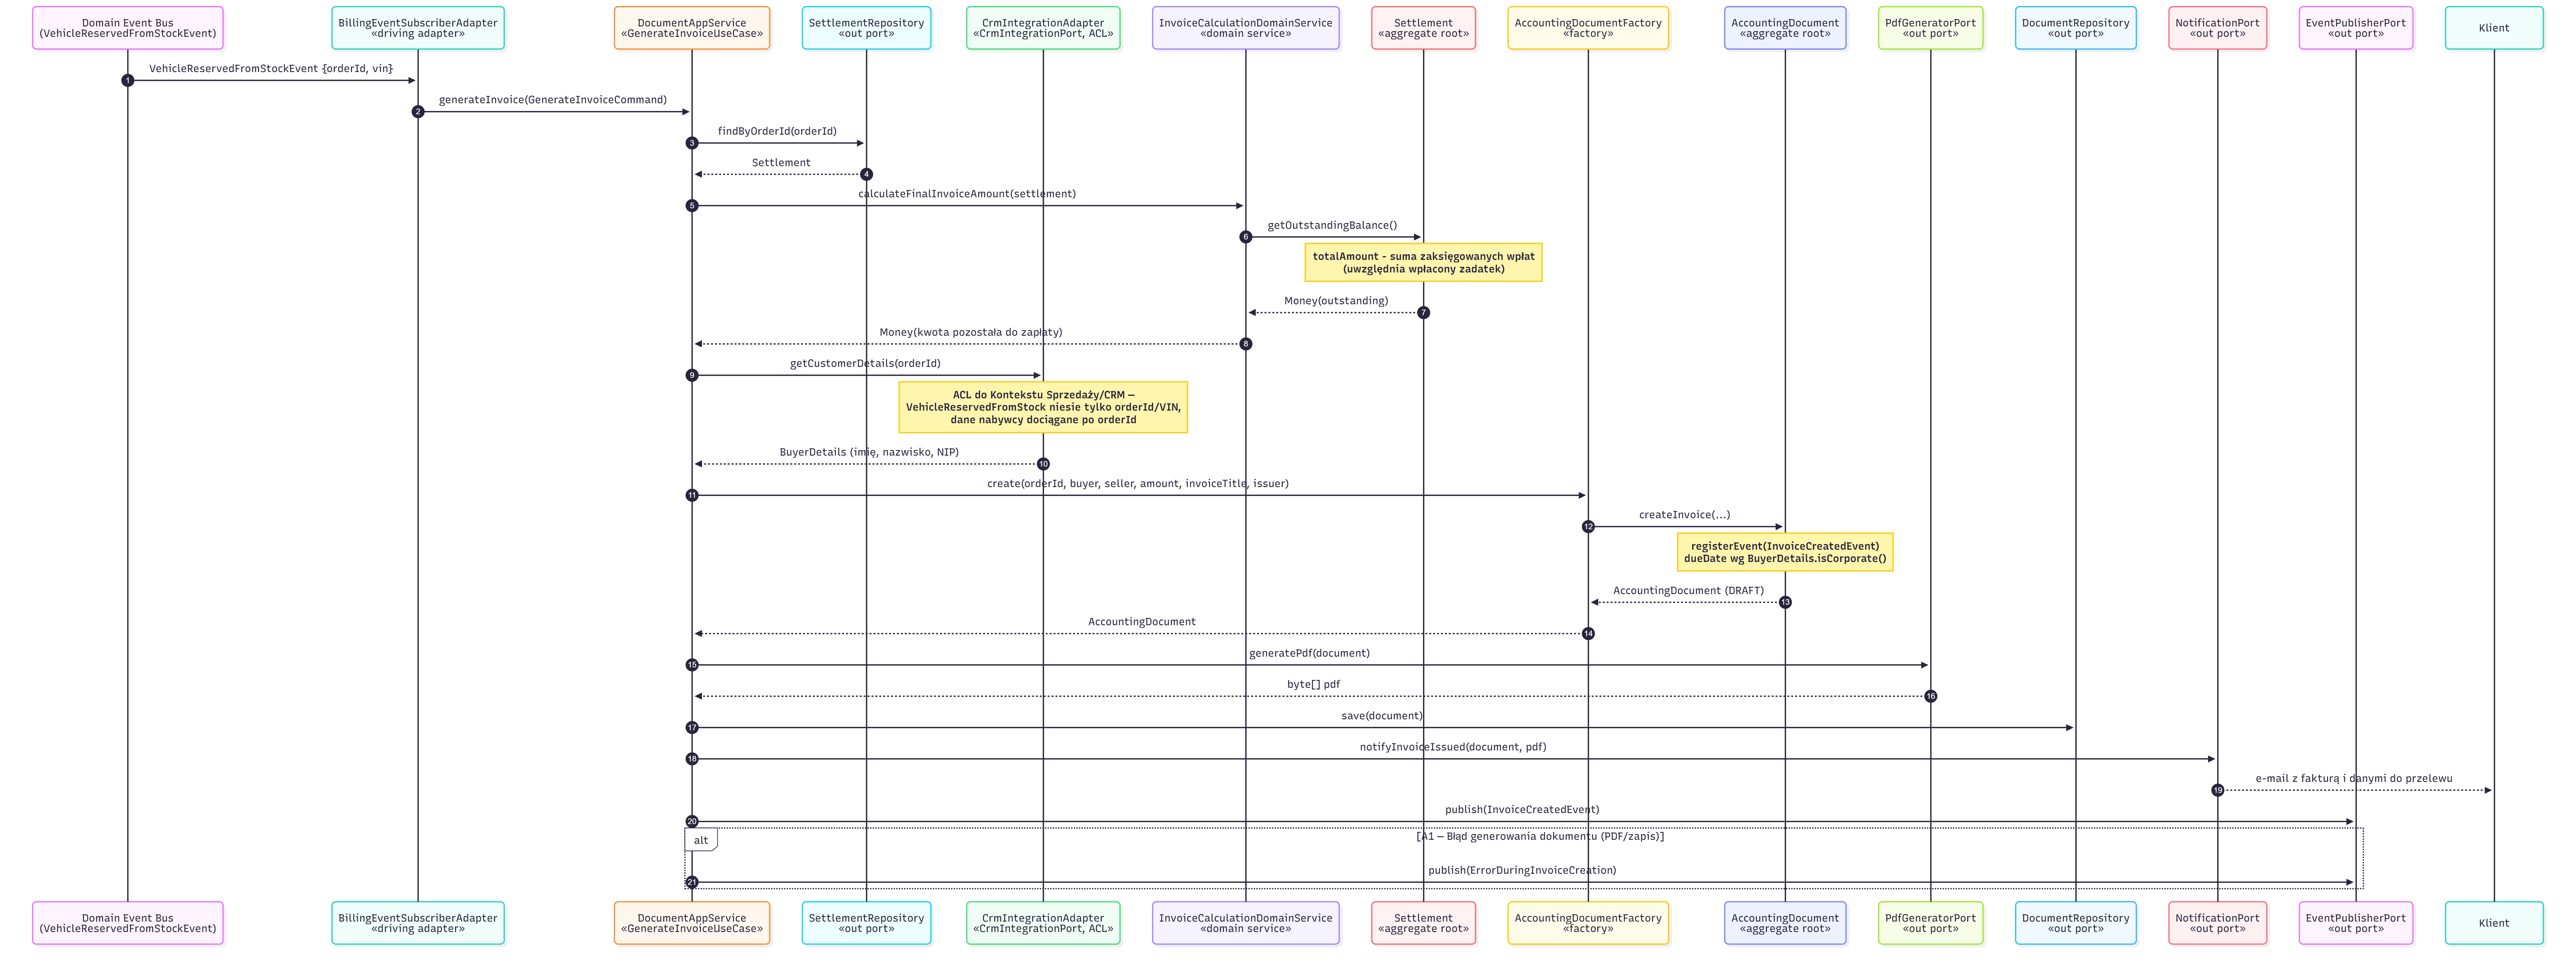
\includegraphics[width=1\textwidth]{media/diagramy_sekwencji/kontekst-faktur-rozliczenia/UC-FIR-02-Sekwencji.png}
    \caption{Diagram sekwencji dla przypadku użycia UC-FIR-02: Stworzenie faktury końcowe}
    \label{fig:seq_uc_fir_02}
\end{figure}

% =====================================================
\textbf{UC-FIR-03: Procesowanie płatności}

\begin{longtable}{|p{4cm}|p{11cm}|}
\hline
\textbf{Element} & \textbf{Opis} \\
\hline

Identyfikator & UC-FIR-03 \\
\hline

Nazwa & Procesowanie płatności \\
\hline

Opis & 
Zaksięgowanie przelewu bankowego i rozliczenie salda zamówienia. \\
\hline

Aktor główny & Księgowy \\
\hline

Aktorzy pomocniczy & System fakturowania \\
\hline

Warunki wstępne & 
W lokalnej bazie istnieje otwarta należność, księgowy zidentyfikował wpłatę na wyciągu. \\
\hline

Warunki końcowe & 
Płatność zarejestrowana, saldo zamówienia zaktualizowane, emitowane \textit{PaymentRegistered} (ewent. \textit{SettlementCompleted}). \\
\hline

Scenariusz główny & 
\begin{enumerate}
    \item Księgowy importuje plik wyciągu bankowego do systemu.
    \item System paruje przelew z zamówieniem (po tytule/ID). W przypadku braku dopasowania automatycznego, księgowy dokonuje weryfikacji ręcznej.
    \item System aktualizuje status płatności na 'SETTLED'.
    \item Kontekst emituje zdarzenie \textit{PaymentRegistered}.
    \item System weryfikuje sumę wpłat. Jeśli saldo = 0 PLN, kontekst emituje \textit{SettlementCompleted}.
\end{enumerate} \\
\hline

Scenariusze alternatywne & 
\begin{itemize}
    \item [A1] Błędna kwota: Kwota wpłaty różni się od wymaganej, system księguje częściowo, status płatności to \textit{PARTIAL\_PAYMENT}.
\end{itemize} \\
\hline
\end{longtable}

\begin{figure}[H]
    \centering
    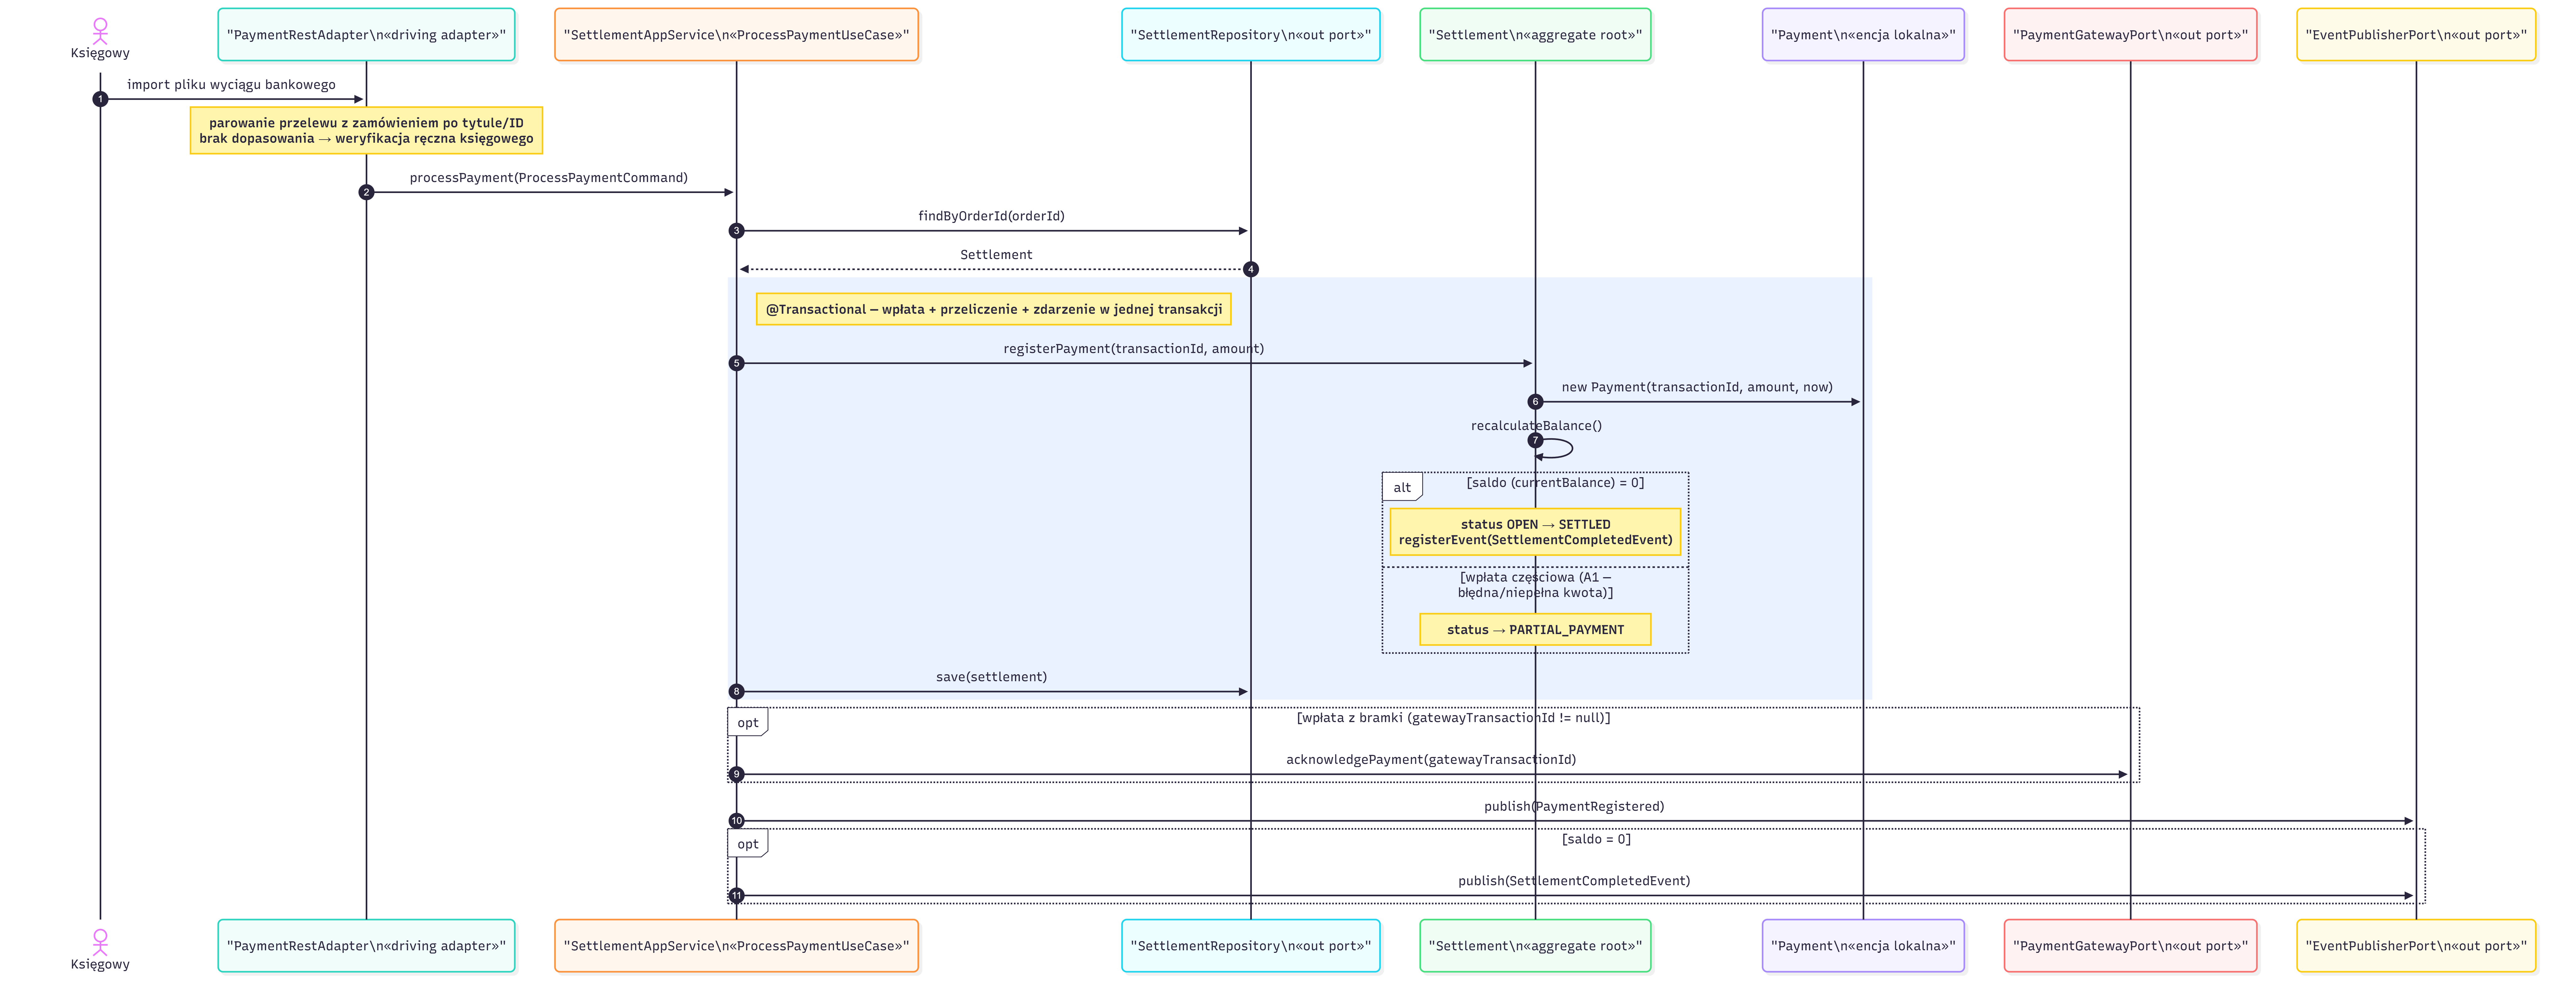
\includegraphics[width=1\textwidth]{media/diagramy_sekwencji/kontekst-faktur-rozliczenia/UC-FIR-03-Sekwencji.png}
    \caption{Diagram sekwencji dla przypadku użycia UC-FIR-03: Procesowanie płatności}
    \label{fig:seq_uc_fir_03}
\end{figure}

\subsubsection{Architektura Kontekstu Fakturowania i Rozliczeń}

Kontekst Fakturowania i Rozliczeń został zaprojektowany w oparciu o architekturę heksagonalną. Diagram Architektury przedstawiono na rysunku \ref{fig:hex_billing}.

\begin{figure}[H]
    \centering
    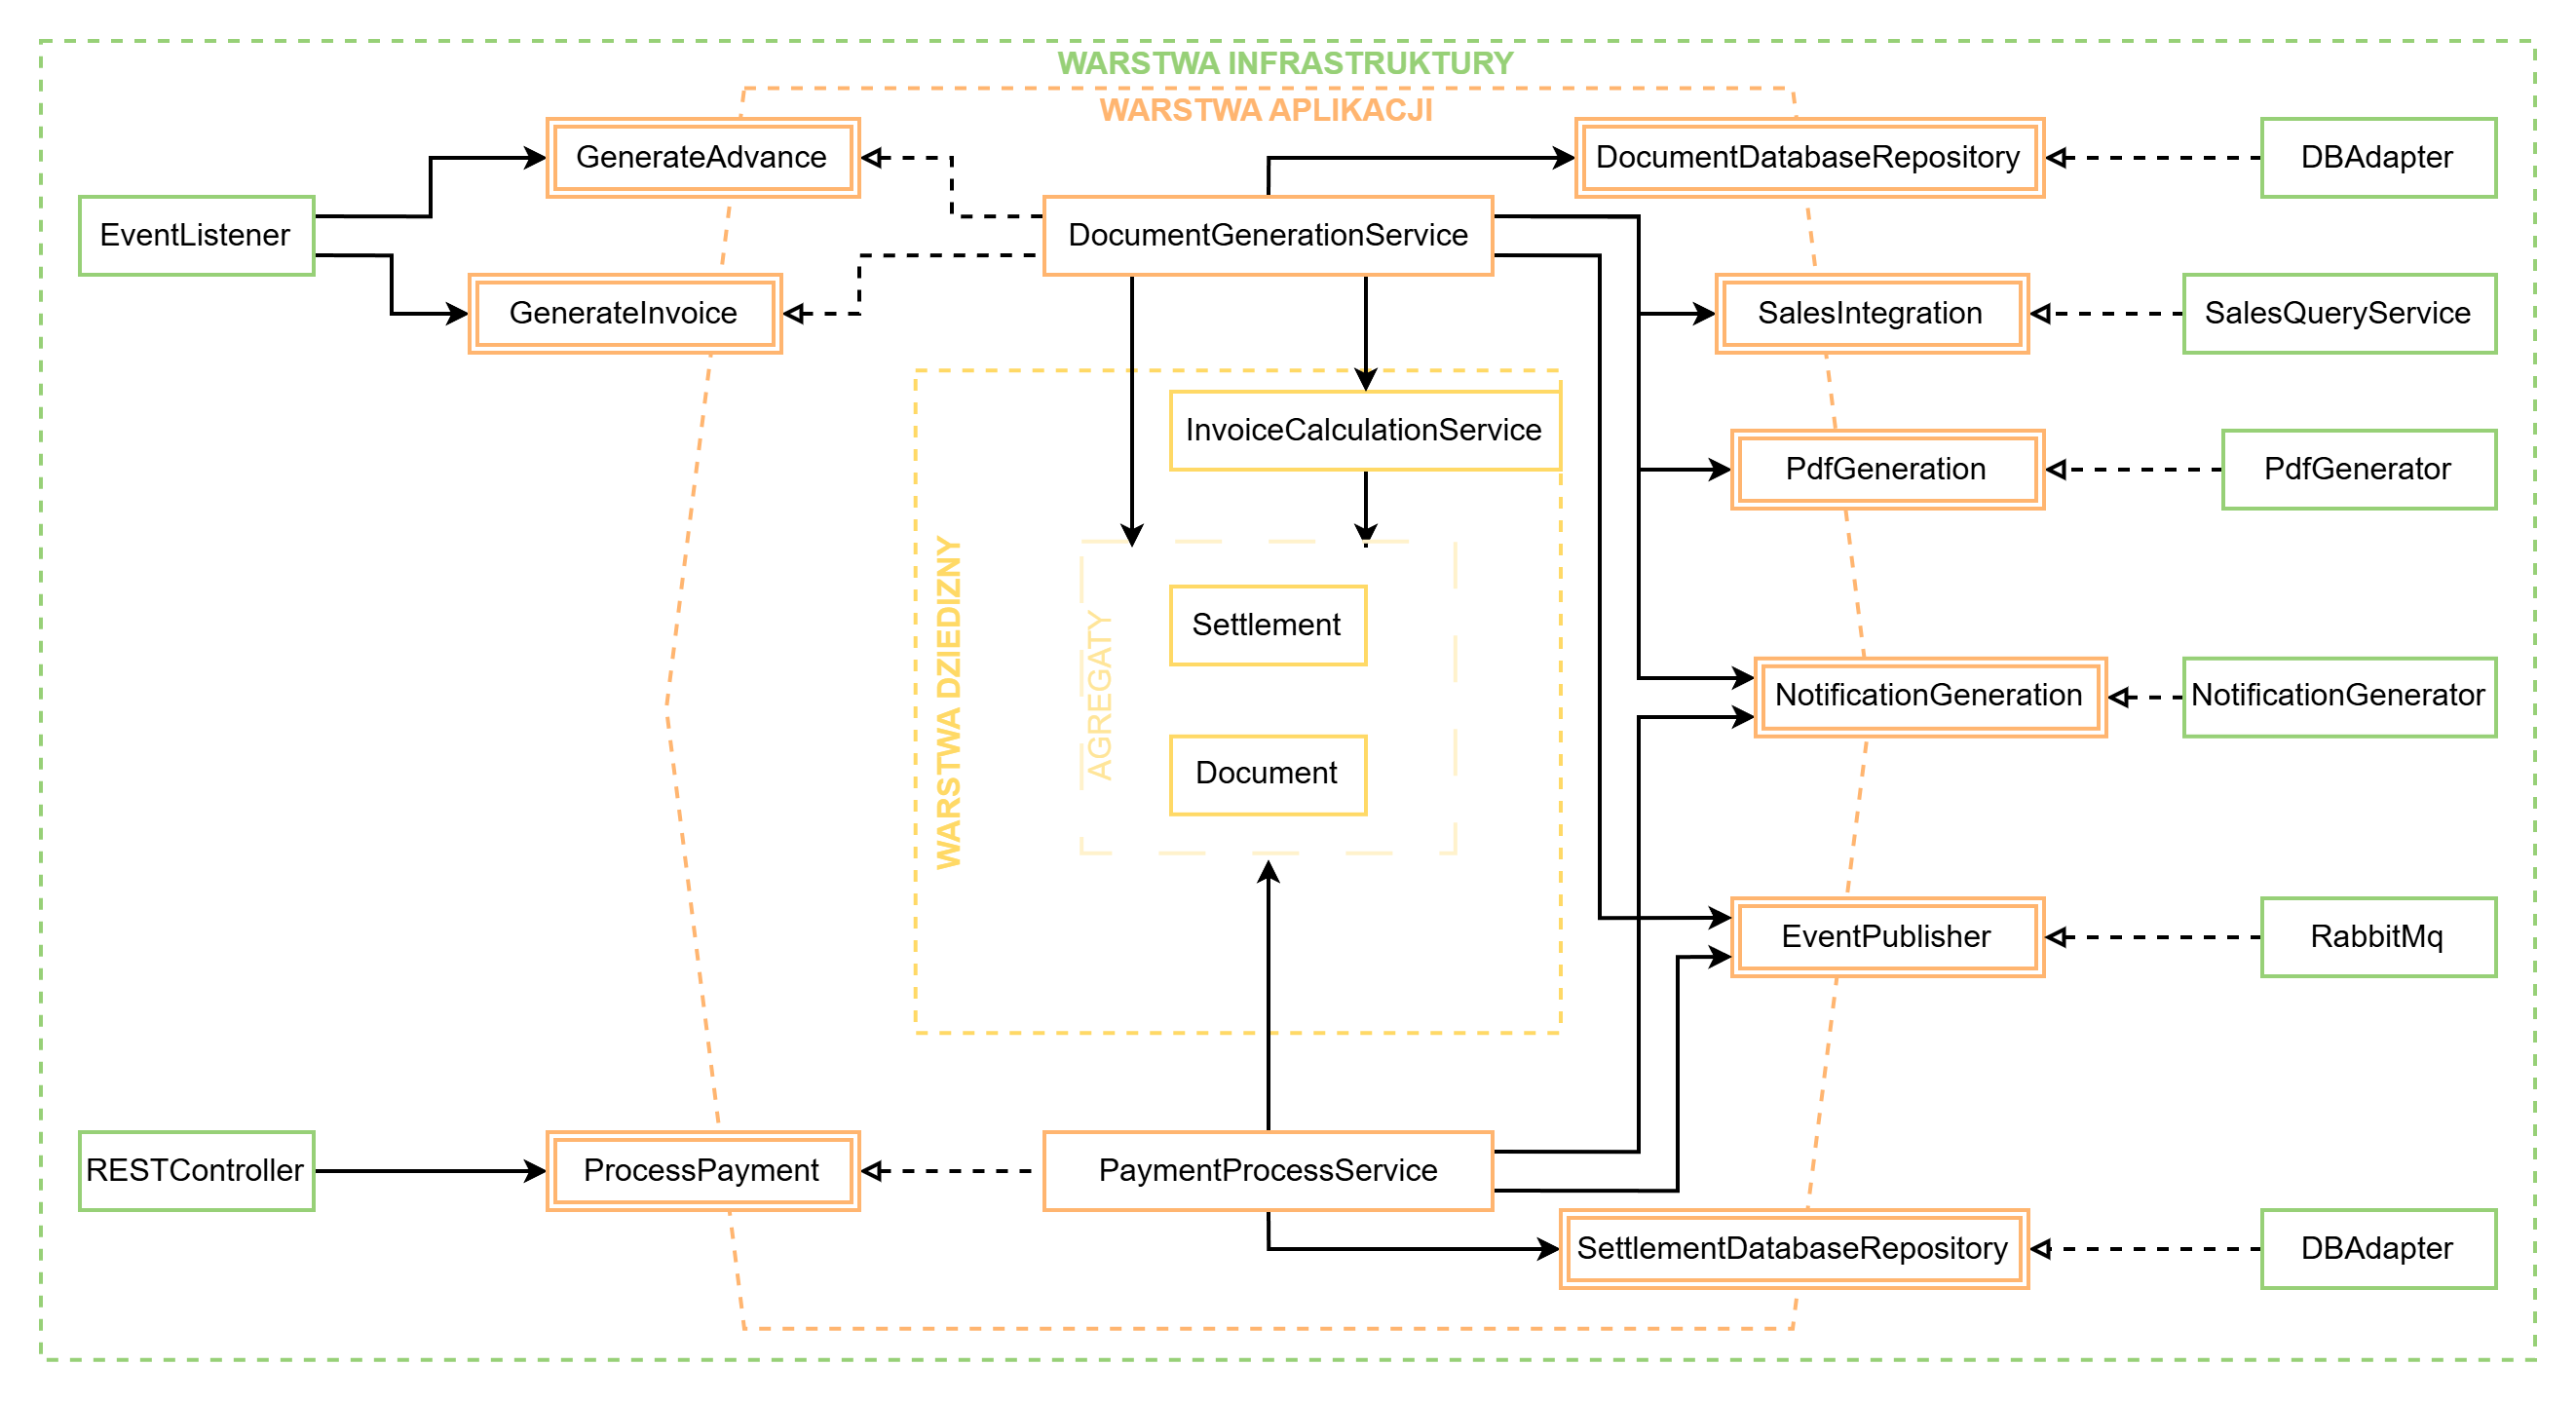
\includegraphics[width=1\linewidth]{media/architektura_heksagonalna/BillingArchitecture.png}
    \caption{Architektura heksagonalna kontekstu fakturowania i rozliczeń}
    \label{fig:hex_billing}
\end{figure}

Poniżej przedstawiono szczegółowy opis interakcji pomiędzy warstwami, z podziałem na strony wejściową i wyjściową.

\paragraph{Strona Wejściowa: Porty i Adaptery} 
Ta strona heksagonu definiuje, w jaki sposób świat zewnętrzny komunikuje się z Kontekstem Fakturowania w celu wyzwolenia konkretnych procesów biznesowych. Aby zachować spójność, interfejsy wejściowe zestawiono bezpośrednio z ich technicznymi implementacjami.

\begin{itemize}
    \item \textbf{Generowanie Dokumentów Finansowych (Asynchroniczne)}
    \begin{itemize}
        \item \textbf{Porty:} \texttt{GenerateAdvance} (wystawienie prośby o zadatek, UC-FIR-01) oraz \texttt{GenerateInvoice} (wystawienie faktury końcowej, UC-FIR-02). Oba interfejsy realizowane są przez jedną usługę aplikacyjną \texttt{DocumentGenerationService}.
        \item \textbf{Adapter:} \texttt{BillingEventSubscriberAdapter} (Messaging Adapter). Nasłuchuje na globalnej magistrali zdarzeń i przechwytuje zdarzenia logistyczne z Inwentarza (odpowiednio: \texttt{VehicleIsNotOnStock} oraz \texttt{VehicleReservedFromStock}), tłumaczy je na komendy (\texttt{GenerateAdvanceCommand}/\texttt{GenerateInvoiceCommand}) i asynchronicznie wyzwala powyższe porty.
    \end{itemize}

    \item \textbf{Zarządzanie Saldem i Wpłatami}
    \begin{itemize}
        \item \textbf{Port:} \texttt{ProcessPayment}. Interfejs obsługujący cykl życia salda (inicjalizacja, zaksięgowanie przelewu — UC-FIR-03 — oraz przypomnienia o płatności), realizowany przez \texttt{PaymentProcessService}.
        \item \textbf{Adaptery:} \texttt{SettlementEventListener} (Messaging Adapter) — nasłuchuje zdarzenia \texttt{OrderReadyForSettlement} z Kontekstu Sprzedaży i inicjalizuje saldo (\texttt{initializeSettlement}), realizując deduplikację po identyfikatorze zdarzenia; oraz \texttt{PaymentReminderCronJobAdapter} (Scheduling Adapter) — cyklicznie wyzwala wysyłkę przypomnień o niezapłaconych saldach (\texttt{sendPaymentReminders}). Ręczne zaksięgowanie wyciągu bankowego (\texttt{processPayment}, węzeł \texttt{RESTController} na diagramie) jest w obecnej implementacji obsługiwane przez warstwę aplikacji i pokryte testami; dedykowany adapter HTTP nie został jeszcze zaimplementowany.
    \end{itemize}
\end{itemize}

\paragraph{Strona Wyjściowa: Porty i Adaptery} 
Ta strona heksagonu definiuje, czego aplikacja potrzebuje od bazy danych, innych systemów, czy zewnętrznych bibliotek, aby zrealizować swoje zadanie.

\begin{itemize}
    \item \textbf{Utrwalanie Stanu (Persystencja)}
    \begin{itemize}
        \item \textbf{Porty:} \texttt{SettlementDatabaseRepository} oraz \texttt{DocumentDatabaseRepository}. Umożliwiają zapis i odczyt agregatów (\texttt{Settlement}, \texttt{AccountingDocument}), indeksowanych po \texttt{OrderId}.
        \item \textbf{Adaptery:} \texttt{InMemorySettlementRepository} oraz \texttt{InMemoryDocumentRepository} (węzeł \texttt{DBAdapter} na diagramie). W bieżącej implementacji są to atrapy przechowujące agregaty w pamięci (typu trwały magazyn); docelowo zostaną zastąpione adapterem bazodanowym (ORM/Hibernate) bez zmiany kontraktu portów.
    \end{itemize}

    \item \textbf{Integracja Międzykontekstowa (Anti-Corruption Layer)}
    \begin{itemize}
        \item \textbf{Port:} \texttt{SalesIntegration}. Query Port służący do synchronicznego dociągania danych nabywcy na podstawie \texttt{OrderId}.
        \item \textbf{Adapter:} \texttt{SalesCrmIntegrationAdapter}. Zależy wyłącznie od publicznej fasady Sprzedaży (\texttt{SalesQueryFacade}, Język Opublikowany), odbiera migawkę \texttt{CustomerSnapshotDto} i tłumaczy ją na hermetyczny obiekt wartości \texttt{BuyerDetails}, chroniąc domenę fakturowania przed korupcją obcymi modelami.
    \end{itemize}

    \item \textbf{Generowanie Plików i Powiadomienia}
    \begin{itemize}
        \item \textbf{Porty:} \texttt{PdfGeneration} oraz \texttt{NotificationGeneration}. Interfejsy zlecające odpowiednio wygenerowanie pliku PDF oraz wysyłkę wiadomości do klienta.
        \item \textbf{Adaptery:} \texttt{PdfGeneratorMockAdapter} (deleguje do metody \texttt{generatePdf()} agregatu \texttt{AccountingDocument}; docelowo wrapper na bibliotekę np. iText/PDFBox) oraz \texttt{NotificationAdapter}/\texttt{NotificationMockAdapter} (atrapy powiadomień konsolowych; docelowo wysyłka e-mail przez serwer SMTP).
    \end{itemize}

    \item \textbf{Publikacja Zdarzeń (Event Driven)}
    \begin{itemize}
        \item \textbf{Port:} \texttt{EventPublisher} (port Wspólnego Jądra). Umożliwia publikację zdarzeń wynikowych na magistralę.
        \item \textbf{Adapter:} \texttt{RabbitMqEventPublisherAdapter} (Wspólne Jądro) w uruchomieniu produkcyjnym lub \texttt{InProcessEventPublisherAdapter} (atrapa w procesie) w demach i testach. Odpowiada za serializację zdarzeń dziedzinowych (np. \texttt{InvoiceCreatedEvent}, \texttt{SettlementCompletedEvent}) i wysłanie ich na magistralę, domykając cykl komunikacji asynchronicznej.
    \end{itemize}
\end{itemize}

\paragraph{Usługi Aplikacji} 
Dla kontekstu Fakturowania i Rozliczeń, jako główne elementy orkiestrujące przepływ między portami wejściowymi a wyjściowymi, przewidziano:
\begin{itemize}
    \item \textbf{DocumentGenerationService} – realizuje orkiestrację dla UC-FIR-01 i UC-FIR-02. Pobiera dane o kliencie przez port CRM, wywołuje fabrykę dokumentów, zleca generowanie pliku PDF, notyfikuje użytkownika, zapisuje agregat \texttt{AccountingDocument} w bazie i emituje odpowiednie zdarzenia.
    \item \textbf{PaymentProcessService} – realizuje orkiestrację dla UC-FIR-03 w celu przetworzenia wpłaty klienta. Pobiera odpowiedni agregat \texttt{Settlement}, przekazuje mu parametry przelewu i publikuje zdarzenia.
\end{itemize}

\paragraph{Usługi Domenowe} 
Dla kontekstu Fakturowania i Rozliczeń, w celu ochrony czystości usług aplikacyjnych, wyodrębniono:
\begin{itemize}
    \item \textbf{InvoiceCalculationService} – bezstanowy serwis hermetyzujący zaawansowaną matematykę finansową. Zamyka w sobie logikę obliczania wysokości wymaganego zadatku (dla UC-FIR-01) oraz wyliczania ostatecznego salda pozostałego do zapłaty na fakturze końcowej (po uwzględnieniu historycznych wpłat dla UC-FIR-02).
\end{itemize}

% Poniżej przedstawiono szczegółowy opis interakcji pomiędzy warstwami oraz uzasadnienie wysoce izolowanego modelu modelowania taktycznego.

% \paragraph{Zarządzanie Wpłatami UC-FIR-03:}
% Ten segment systemu odpowiada za matematykę finansową i ewidencję wpłat. Zaprojektowano go tak, aby zagwarantować pełną spójność transakcyjną.
% \begin{itemize}
%     \item \textbf{Inicjalizacja:} Złożenie nowego zamówienia wyzwala port wejściowy, który poprzez usługę \linebreak \texttt{SettlementAppService} oddelegowuje zadanie do \texttt{SettlementFactory}. Fabryka powołuje do życia agregat salda na podstawie zamówienia uzyskanego w zdarzeniu.
%     \item \textbf{Rejestracja wpłaty:} Kiedy księgowy wgrywa wyciąg bankowy, port \texttt{ProcessPaymentUseCase} wysyła żądanie do usługi aplikacyjnej. Usługa pobiera agregat \texttt{Settlement} z bazy i wywołuje na nim mutację stanu. Pojedyncza wpłata nie posiada własnego repozytorium – jest enkapsulowana i zapisywana jako element kolekcji wewnątrz agregatu. Gwarantuje to, że wyliczenie salda zerowego i ewentualna emisja zdarzenia \texttt{SettlementCompletedEvent} zachodzą zawsze w jednej, bezpiecznej transakcji bazodanowej.
% \end{itemize}

% \paragraph{Wystawianie Faktur UC-FIR-01 i UC-FIR-02:}
% Segment ten zarządza generowaniem prawnie wiążących dokumentów PDF zadatku oraz faktury końcowej. Osiągnięto tu pełną izolację logiki wyliczeniowej od infrastruktury.
% \begin{itemize}
%     \item \textbf{Czystość Usługi Aplikacyjnej i Pobieranie Danych:} \texttt{DocumentAppService} pełni wyłącznie rolę kierownika przepływu. Nie zawiera instrukcji warunkowych ani operacji matematycznych. Odpowiada za koordynację wywołań pomiędzy domeną a portami wyjściowymi – w tym za synchroniczne odpytanie zewnętrznego kontekstu Sprzedaży i CRM poprzez port wyjściowy \texttt{CrmIntegrationPort} w celu dociągnięcia pełnych danych teleadresowych nabywcy (\texttt{BuyerDetails}) przed przystąpieniem do kreacji dokumentu. Zapobiega to niespójnościom wynikającym z faktu, że zdarzenia logistyczne z placu nie zawierają w sobie wrażliwych danych osobowych klientów.
%     \item \textbf{InvoiceCalculationDomainService} Wprowadzenie tego bezstanowego serwisu chroni warstwę aplikacji przed wyciekiem reguł biznesowych. Ponieważ wyliczenie ostatecznej kwoty faktury wymaga odjęcia zaksięgowanych wpłat od wartości kontraktu, serwis domenowy w sposób kontrolowany uzyskuje informacje ze stanu agregatu \texttt{Settlement}. Wylicza on kwotę i zwraca czysty obiekt wartości. Rozwiązanie to drastycznie zwiększa testowalność skomplikowanej matematyki księgowej.
%     \item \textbf{Bezpieczna Fabryka Dokumentu:} Gotowa kwota obliczona przez serwis domenowy przekazywana jest przez orkiestratora do \texttt{AccountingDocumentFactory}. Fabryka ta, łącząc kalkulacje finansowe z pobranym wcześniej z portu obiektem \texttt{BuyerDetails}, zajmuje się walidacją terminów płatności i zwraca poprawny, w pełni zainicjalizowany agregat \texttt{AccountingDocument}.
% \end{itemize}

% \paragraph{Porty Wyjściowe i Zdarzenia:} Do realizacji powyższych celów potrzebne również są porty realizujące poniższe zadania:
% \begin{itemize}
%     \item \textbf{NotificationPort} i \textbf{PdfGeneratorPort}: Zamiast implementować biblioteki do obsługi protokołu SMTP czy generowania plików PDF bezpośrednio w logice aplikacji, zdefiniowano interfejsy. Konkretne adaptery zostaną wstrzyknięte w zewnętrznym pierścieniu infrastruktury.
%     \item \textbf{CrmIntegrationPort:} Międzykontekstowy port wyjściowy typu Query. Odpowiada za synchroniczne pobranie danych tożsamościowych i skarbowych klienta z modułu CRM na podstawie \texttt{OrderId}. Użycie dedykowanego portu zapewnia zgodność z regulacjami RODO, izolując dane osobowe od globalnej magistrali komunikatów logistycznych.
%     \item \textbf{Magistrala Zdarzeń (Domain Event Bus):} Przepływ pracy kończy się wyemitowaniem zdarzeń dziedzinowych (np. \texttt{AdvancePaymentRequested}, \texttt{InvoiceCreated}), co pozwala reszcie systemu (np. modułowi Sprzedaży) na asynchroniczne reagowanie bez tworzenia cyklicznych zależności.
% \end{itemize}

\subsubsection{Agregaty Kontekstu Fakturowania i Rozliczeń}

Model taktyczny tego kontekstu został zdekomponowany na dwa agregaty. Taki podział eliminuje ryzyko blokad bazy danych (np. podczas jednoczesnej rejestracji wpłaty przez bramkę online i wystawiania faktury przez księgowość).

\begin{figure}[H]
    \centering
    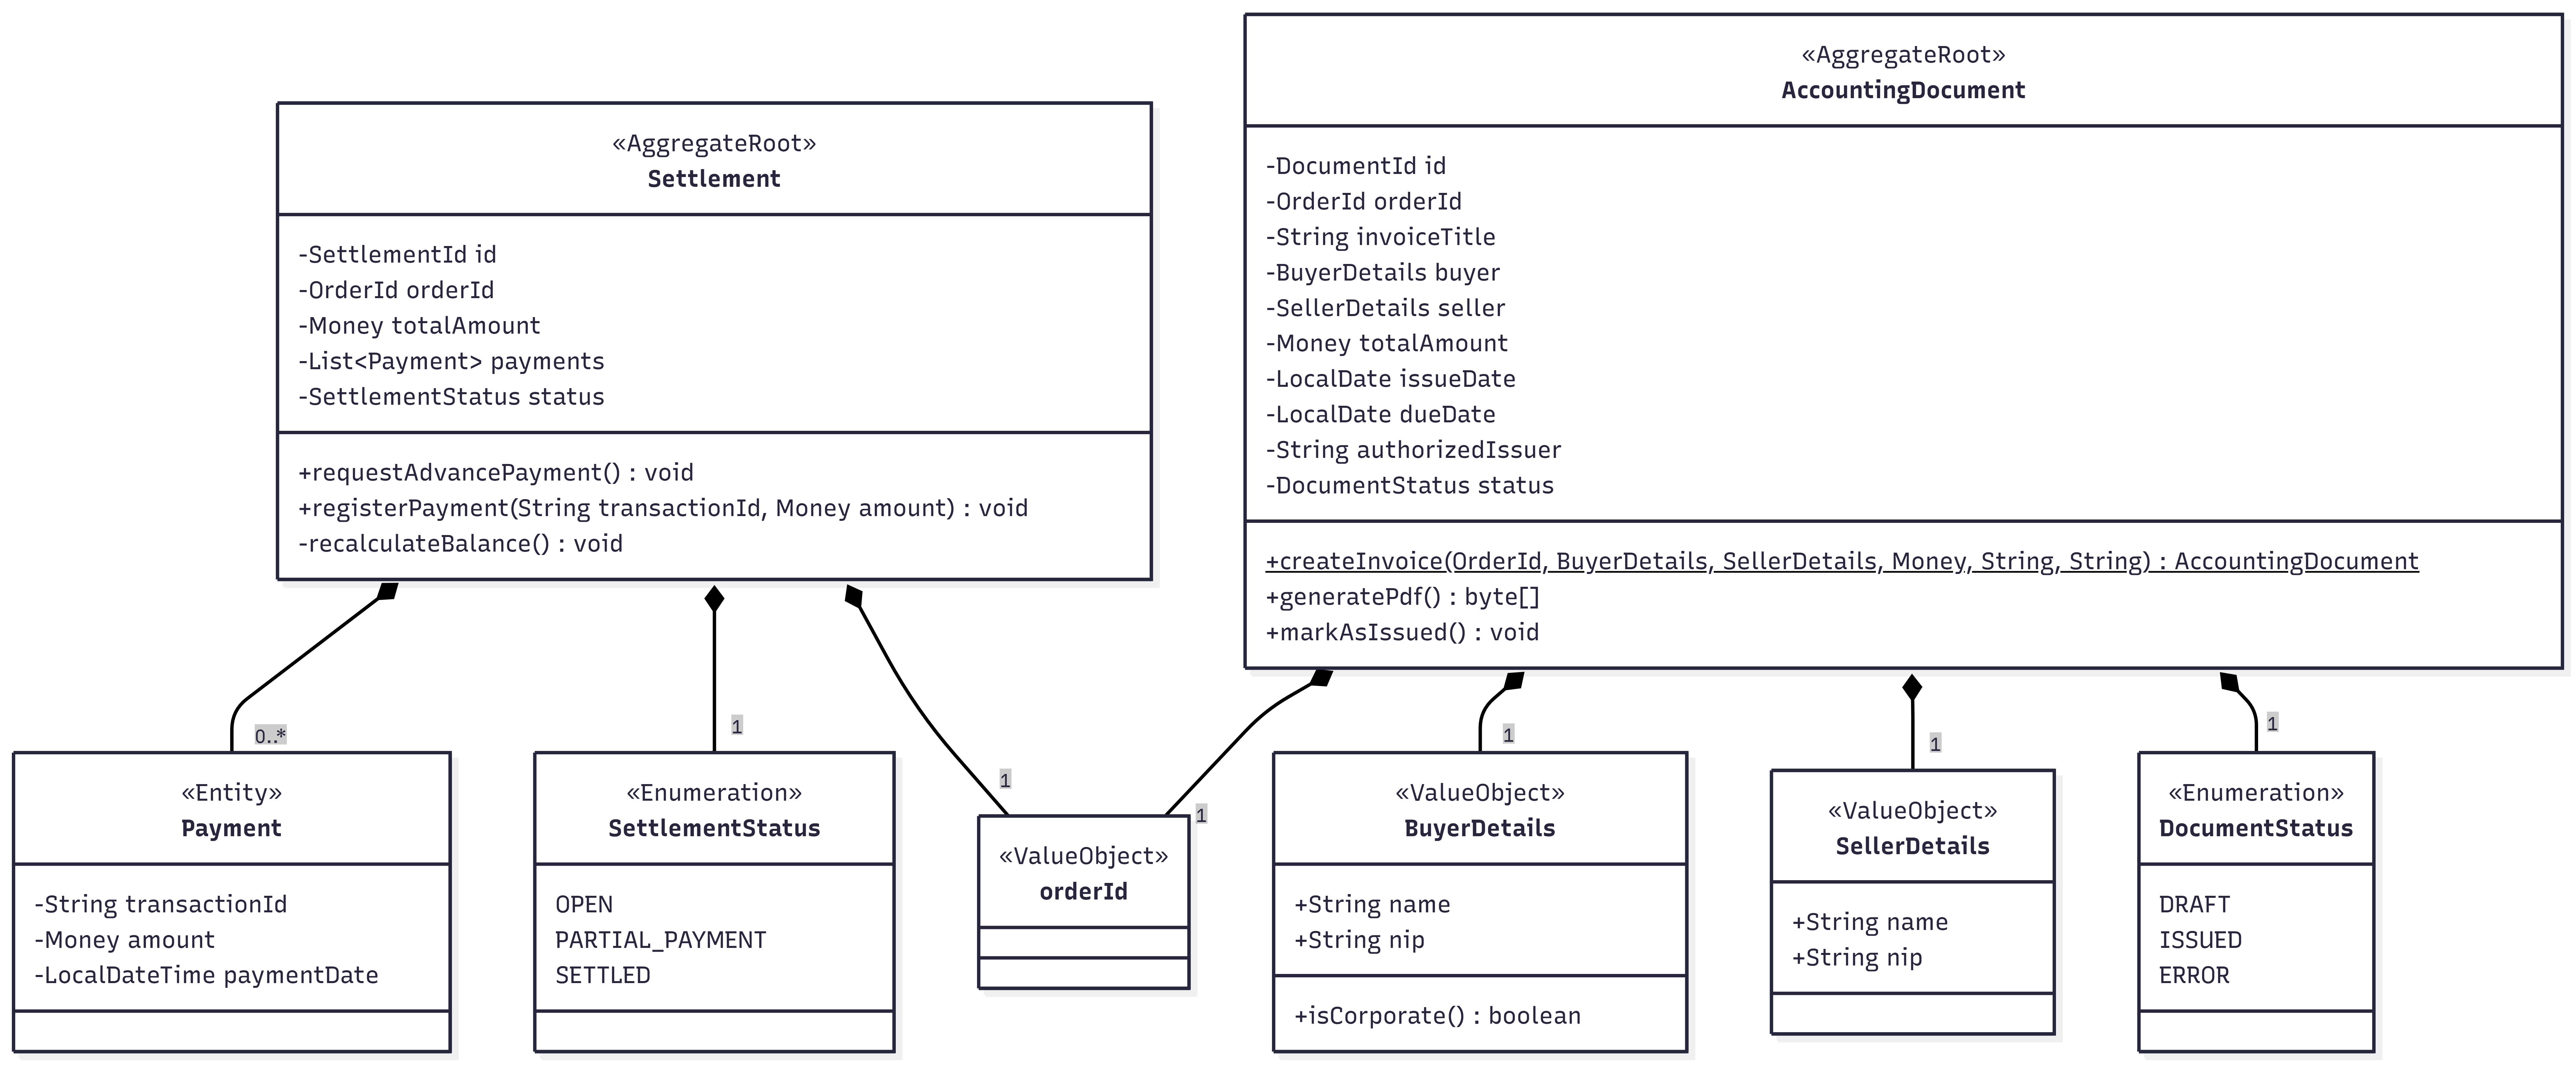
\includegraphics[width=\textwidth]{media/agregaty/kontekst-fakturowania-rozliczen/settlement-document.png}
    \caption{Model strukturalny agregatów kontekstu fakturowania i rozliczeń}
    \label{fig:agg_payment}
\end{figure}

Logika biznesowa została skondensowana wokół dwóch wysoce spójnych agregatów: \texttt{Settlement} oraz \texttt{AccountingDocument}.

\paragraph{Agregat: Settlement (Rozliczenie Zamówienia)}
Agregat ten stanowi centralny mechanizm kontroli finansowej dla konkretnego kontraktu, powiązany z nim poprzez niemutowalny identyfikator \texttt{OrderId}. Zgodnie z podziałem odpowiedzialności, jego wyłącznym zadaniem jest obsługa ewidencji wpłat (Przypadek użycia \textbf{UC-FIR-03}).
\begin{itemize}
    \item \textbf{Encja Lokalna Wpłaty (\texttt{Payment}):} Pojedyncze transakcje z wyciągów bankowych nie posiadają globalnej tożsamości. Są one traktowane jako encje lokalne wewnątrz agregatu \texttt{Settlement}. Gwarantuje to, że wpłata nie może istnieć w systemie w oderwaniu od przypisanego do niej zamówienia.
    \item \textbf{Ochrona Niezmienników:} Agregat jest wyłącznym właścicielem reguł matematycznych. Rejestracja nowej wpłaty (metoda \texttt{registerPayment}) powoduje dodanie jej do wewnętrznej kolekcji oraz natychmiastowe, ukryte przeliczenie pola \texttt{currentBalance} względem całkowitej wartości kontraktu \texttt{totalAmount} (wewnętrzna metoda \texttt{recalculateBalance}). 
    \item \textbf{Autonomiczna Zmiana Stanu:} Na podstawie wyliczonego bieżącego bilansu, agregat samodzielnie podejmuje decyzję o zmianie statusu z \texttt{OPEN} na \texttt{PARTIAL\_PAYMENT} lub \texttt{SETTLED}. Osiągnięcie zerowego zadłużenia (\texttt{currentBalance} = 0) skutkuje natychmiastową kreacją wewnątrz agregatu zdarzenia \texttt{SettlementCompletedEvent}, które zamyka proces rozliczenia.
\end{itemize}

\paragraph{Agregat: AccountingDocument (Dokument Księgowy)}
Agregat odpowiedzialny za procesowanie prawnie wiążących dokumentów skarbowych (zarówno Faktur Końcowych, jak i Proform). Przejęcie pełnej odpowiedzialności za oficjalną komunikację finansową sprawia, że wspiera on realizację aż dwóch przypadków użycia: \textbf{UC-FIR-01} (prośba o zadatek) oraz \textbf{UC-FIR-02} (faktura końcowa). Oddzielenie go od agr


\end{document}